
\documentclass [PhD] {uclathes}

\usepackage{graphicx}
\usepackage{amsmath}
\usepackage{amsfonts}
\usepackage[usenames,dvipsnames]{xcolor}
\definecolor{linkcolor}{RGB}{0,0,102}
\usepackage{hyperref} 
\hypersetup{
	pdfstartview = {XYZ},
	colorlinks,
	allcolors = linkcolor,
	bookmarksopen,
	bookmarksnumbered
}
\usepackage{setspace}
\usepackage{silence}
\WarningFilter{caption}{Unknown} % captionpackage complains about thesis document class
\usepackage{caption}
\captionsetup{font={stretch=1}}
\usepackage{tabularx, colortbl}
\definecolor{mygray}{gray}{0.9}
\def \figscale {0.28}
\usepackage{multicol}
\usepackage{soul}
%%%%%%%%%%%%%%%%%%%%%%%%%%%%%%%%%%%%%%%%%%%%%%%%%%%%%%%%%%%%%%%%%%%%%%
%
% Usually things live in separate flies.
%
% \input {prelim}                           % preliminary page info

%%%%%%%%%%%%%%%%%%%%%%%%%%%%%%%%%%%%%%%%%%%%%%%%%%%%%%%%%%%%%%%%%%%%%%%%
%                                                                      %
%                          PRELIMINARY PAGES                           %
%                                                                      %
%%%%%%%%%%%%%%%%%%%%%%%%%%%%%%%%%%%%%%%%%%%%%%%%%%%%%%%%%%%%%%%%%%%%%%%%

\title          {Identifying genomic regulatory patterns \\
                 underlying complex phenotypes from heterogeneous data}
\author         {Brandon Jew}
\department     {Bioinformatics}
% Note:  degreeyear should be optional, but as of  5-Feb-96
% it seems required or you get a year of ``2''.   -johnh
\degreeyear     {2021}

%%%%%%%%%%%%%%%%%%%%%%%%%%%%%%%%%%%%%%%%%%%%%%%%%%%%%%%%%%%%%%%%%%%%%%%%

\chair          {Eran Halperin}
\chair          {Jae Hoon Sul}
\member         {Päivi Pajukanta}
\member         {Sriram Sankararaman}


%%%%%%%%%%%%%%%%%%%%%%%%%%%%%%%%%%%%%%%%%%%%%%%%%%%%%%%%%%%%%%%%%%%%%%%%

\dedication     {\textsl{To my wife, \\
                my constant source of happiness and inspiration.}}

%%%%%%%%%%%%%%%%%%%%%%%%%%%%%%%%%%%%%%%%%%%%%%%%%%%%%%%%%%%%%%%%%%%%%%%%

\acknowledgments {First and foremost, I thank my advisors, Eran Halperin and Jae Hoon Sul. I am extremely grateful to have both as amazing mentors who provided me with exciting projects and opportunities to grow as a researcher. They both fostered welcoming and top-notch research groups that I am proud to be a part of. My \textsl{Halperin Lab} fleece jacket and \textsl{Sul Lab} mug will always be parts of my look as a scientist.   

I would also like to thank Eleazar Eskin, who roped me into bioinformatics in the first place and supported me through my PhD. Much of my work was done with Päivi Pajukanta, Noah Zaitlen, and Sriram Sankararaman. I am extremely grateful for their collaboration and mentorship. I thank Lana Martin and Robert Smith, who helped me immensely with funding and outreach projects during their time in Eleazar’s lab. I thank Sim-Lin Lau and Margaret Chu for their amazing support.

Many thanks to my lab mates in Eran's lab (Elior, Mike, Leah, Johnson, Liat, Ulzee, Brian, Nadav, Jeff) and Jae Hoon's Lab (Albert, Sarah, Lingyu). Also thanks to our shared lab space friends from Sriram's lab (Alec, Chris, Ruthie, Arun, Ariel, Ali). I really enjoyed talking too much during work hours and tracking down every opportunity for free food. 

Finally, I would like to thank my family for their unwavering support. I thank my wife, the amazing Dr. Maegan Lu. Over the past 8 years, she's been a constant source of support and inspiration to move forward. \\
%\\
%Chapter Two of this dissertation is a version of Brandon Jew, Marcus Alvarez, Elior Rahmani, Zong Miao, Arthur Ko, Kristina M. Garske, Jae Hoon Sul, Kirsi H. Pietiläinen, Päivi Pajukanta, Eran Halperin. Accurate estimation of cell composition in bulk expression through robust integration of single-cell information. \textsl{Nature Communications.} 2020.

%Chapter Three is a version of Brandon Jew, Jiajin Li, Sriram Sankararaman, Jae Hoon Sul. An efficient linear mixed model framework for meta-analytic association studies across multiple contexts. \textsl{To appear in WABI 2021}.

%Chapter Four is a version of Brandon Jew, Jae Hoon Sul, Noah Zaitlen. Selection contributes to skewed X chromosome inactivation across human tissues. \textsl{In preparation}.


This work was supported by the National Science Foundation Graduate Research Fellowship Program under Grant No. DGE-1650604.

}

%%%%%%%%%%%%%%%%%%%%%%%%%%%%%%%%%%%%%%%%%%%%%%%%%%%%%%%%%%%%%%%%%%%%%%%%

\vitaitem   {2017-2021}
                {PhD, Bioinformatics, University of California, Los Angeles, CA, USA}
\vitaitem   {2018-2021}
                {Graduate Research Fellow, National Science Foundation}
\vitaitem   {2013--2017}
                {BS, Biochemistry (minor in Bioinformatics), University of California, Los Angeles, CA, USA}
\vitaitem   {2014-2016}
                {Research Assistant, Loo Laboratory, University of California, Los Angeles, CA, USA}
\vitaitem   {2014}
                {Research Intern, Evans Laboratory, Salk Institute for Biological Studies}

%%%%%%%%%%%%%%%%%%%%%%%%%%%%%%%%%%%%%%%%%%%%%%%%%%%%%%%%%%%%%%%%%%%%%%%%
            
  \publication{* Denotes equal contribution}
  \publication{Aditya Gorla, \textbf{Brandon Jew}, Luke Zhang, Jae Hoon Sul. xGAP: A python based efficient, modular, extensible and fault tolerant genomic analysis pipeline for variant discovery. \textsl{Bioinformatics.} 2021.}
  \publication {David Goodman-Meza, Akos Rudas, Jeffrey N Chiang, Paul C Adamson, Joseph Ebinger, Nancy Sun, Patrick Botting, Jennifer A Fulcher, Faysal G Saab, Rachel Brook, Eleazar Eskin, Ulzee An, Misagh Kordi, \textbf{Brandon Jew}, Brunilda Balliu, Zeyuan Chen, Brian L Hill, Elior Rahmani, Eran Halperin, Vladimir Manuel. A machine learning algorithm to increase COVID-19 inpatient diagnostic capacity. \textsl{PLoS One.} 2020.}
  \publication {Zong Miao, Marcus Alvarez, Arthur Ko, Yash Bhagat, Elior Rahmani, \textbf{Brandon Jew}, Sini Heinonen, Karen L Mohlke, Markku Laakso, Kirsi H. Pietiläinen, Eran Halperin, Päivi Pajukanta. The causal effect of obesity on prediabetes and insulin resistance reveals the important role of adipose tissue in insulin resistance. \textsl{PLoS Genetics.} 2020.}
  \publication {Marcus Alvarez*, Elior Rahmani*, \textbf{Brandon Jew}, Kristina M Garske, Zong Miao, Jihane N Benhammou, Chun Jimmie Ye, Joseph R Pisegna, Kirsi H Pietiläinen, Eran Halperin, Päivi Pajukanta. Enhancing droplet-based single-nucleus RNA-seq resolution using the semi-supervised machine learning classifier DIEM. \textsl{Scientific Reports}. 2020.}
  \publication {\textbf{Brandon Jew}*, Marcus Alvarez*, Elior Rahmani, Zong Miao, Arthur Ko, Kristina M. Garske, Jae Hoon Sul, Kirsi H. Pietiläinen, Päivi Pajukanta, Eran Halperin. Accurate estimation of cell composition in bulk expression through robust integration of single-cell information. \textsl{Nature Communications.} 2020.}
    \presentation{\textbf{Brandon Jew}, Marcus Alvarez, Elior Rahmani, Zong Miao, Arthur Ko, Kristina M. Garske, Jae Hoon Sul, Kirsi H. Pietiläinen, Päivi Pajukanta, Eran Halperin. Accurate estimation of cell composition in bulk expression through robust integration of single-cell information. Platform presented at the 69th Annual Meeting of the American Society of Human Genetics, October 19, 2019, Houston, Texas.}
  \publication {Jennifer Zou, Farhad Hormozdiari, \textbf{Brandon Jew}, Stephane E Castel, Tuuli Lappalainen, Jason Ernst, Jae Hoon Sul, Eleazar Eskin. Leveraging allelic imbalance to refine fine-mapping for eQTL studies. \textsl{PLoS Genetics.} 2019.}
  \publication {Brian L Hill, Robert Brown, Eilon Gabel, Nadav Rakocz, Christine Lee, Maxime Cannesson, Pierre Baldi, Loes Olde Loohuis, Ruth Johnson, \textbf{Brandon Jew}, Uri Maoz, Aman Mahajan, Sriram Sankararaman, Ira Hofer, Eran Halperin. An automated machine learning-based model predicts postoperative mortality using readily-extractable preoperative electronic health record data. \textsl{British Journal of Anaesthesia.} 2019.}
  \publication {Jiajin Li, \textbf{Brandon Jew}, Lingyu Zhan, Sungoo Hwang, Giovanni Coppola, Nelson B Freimer, Jae Hoon Sul. ForestQC: quality control on genetic variants from next-generation sequencing data using random forest. \textsl{PLoS Computational Biology.} 2019.}
  \publication {\textbf{Brandon Jew}, Jae Hoon Sul. Variant calling and quality control of large-scale human genome sequencing data. \textsl{Emerging Topics in Life Sciences.} 2019.\\}
  
% \customCV{
% \begin{center}
%     SUBMITTED MANUSCRIPTS 
% \end{center}
%   \textbf{Brandon Jew}, Jae Hoon Sul, Noah Zaitlen. Selection contributes to skewed X chromosome inactivation across human tissues. \\
  
%   \noindent \textbf{Brandon Jew}, Jiajin Li, Sriram Sankararaman, Jae Hoon Sul. An efficient linear mixed model framework for meta-analytic association studies across multiple contexts. \\
  
%   \noindent Elior Rahmani*, \textbf{Brandon Jew}*, Eran Halperin. Differential DNA methylation at cell-type resolution: establishing rigorous guidelines.
% }

%%%%%%%%%%%%%%%%%%%%%%%%%%%%%%%%%%%%%%%%%%%%%%%%%%%%%%%%%%%%%%%%%%%%%%%%

\abstract       {Large-scale transcriptomic datasets provide valuable opportunities to better understand the regulation of gene expression and its role in human health. However, these studies can be confounded by issues such as cell type heterogeneity. Furthermore, these datasets are growing extremely large with complex study designs, such as gene expression measured across a multitude of tissues, that must be accurately and efficiently modeled. Finally, better understanding of the mechanisms that influence gene regulation are required to integrate novel associations with biological understanding. In this dissertation, we introduce methods that address these issues in the analysis of tissue-level gene expression data. We present a method to accurately estimate cell type composition from these data by integrating single-cell information, as well as a scalable approach to model multi-tissue expression datasets and identify expression quantitative trait loci. We also present analyses of bulk expression data that validates a hypothesized mechanism of gene regulation that occurs in the general female population through non-random X chromosome inactivation. The work presented in this dissertation allows researchers to perform efficient and accurate analyses of gene expression data and provides additional insight into the mechanisms that underlie associations between genetics, transcriptomics, and complex phenotypes.}

%%%%%%%%%%%%%%%%%%%%%%%%%%%%%%%%%%%%%%%%%%%%%%%%%%%%%%%%%%%%%%%%%%%%%%%%



\begin {document}
\makeintropages

%%%%%%%%%%%%%%%%%%%%%%%%%%%%%%%%%%%%%%%%%%%%%%%%%%%%%%%%%%%%%%%%%%%%%%
%
% Ordinarily each chapter (at least) is in a separate file.
%
%\chapter{Introduction}
\section{Scope of Research}
Advances in sequencing technologies have paved the way for the generation of large-scale genomic datasets capturing genetic and transcriptomic variation across diverse sets of individuals \cite{Bycroft2018, GTEx_Consortium2020-xx}. These data allow researchers to elucidate the relationship between genetics, gene expression, and complex phenotypes \cite{Gusev2016}. Genome-wide association studies have identified a vast number of genetic loci associated with different traits \cite{gwas} and the identification of expression quantitative trait loci (eQTLs) bridges the gap between genotype and phenotype by elucidating the effects of genetic variation on gene expression \cite{Nica2013}. These associations serve as stepping stones for better understanding of human health and potential therapeutic targets \cite{Motsinger-Reif2013, walker2001pharmaceutical}. However, studies involving tissue-level gene expression are hindered by confounding factors that can both decrease power to detect associations and cause spurious results.

Many tissues in the human body consist of several cell types. For example, brain tissue often contains an assortment of neuronal and glial cell populations, each with distinct functions and gene expression profiles. RNA sequencing (RNA-seq) is often performed on whole tissues and analyses of these data can be confounded by cell-type heterogeneity across samples \cite{farahbod2020untangling}. Differences in cell type composition can be misinterpreted as differences in gene expression levels when measuring RNA across tissues. Furthermore, these mixtures can obscure cell-type-specific gene regulation that may be of interest \cite{Westra2015-vq, Shen-Orr2010-tg}. Single-cell approaches, such as single-cell RNA-seq (scRNA-seq) and single-nucleus RNA-seq (snRNA-seq), avoid these issues and provide insight into the gene expression of individual cells. However, these experiments remain costly, noisy, and difficult to scale compared to bulk RNA-seq \cite{lahnemann2020eleven}. Given the continuing utility of tissue-level RNA-seq datasets, it is important to accurately model variability in cell type proportions in these samples.

Regulation of gene expression also varies significantly across tissues \cite{GTEx_Consortium2020-xx}. Moreover, several tissues can have distinct roles in biological systems underlying a complex phenotype. For example, analyses of Type II diabetes have observed transcriptomic changes in blood \cite{Christodoulou2019}, adipose \cite{Miao2020}, and brain \cite{Zhou2019}. Therefore, it is imperative to measure gene expression across many tissues to fully understand gene regulation and its role in traits of interest. Analyzing gene expression across tissues, especially with growing sample sizes, requires approaches that can model this heterogeneity both accurately and efficiently.

Finally, the relationship between gene expression and genetic variation is highly complex \cite{robert2018exploring} and remains to be fully understood. Many eQTLs have been identified and are thought to influence gene expression through interactions with regulatory regions of the genome, such as enhancers and promoters \cite{Garieri2017}. Alternative mechanisms of genetic influences on gene regulation have been hypothesized, specifically in the context of selective pressures causing non-random X chromosome inactivation \cite{Migeon1998-gc}. To better understand human biology, it is important to validate these hypotheses and identify the extent of their influence on regulation of gene expression. 

\section{Contributions and Overview}
In this dissertation, we introduce computational and statistical methods to accurately model tissue-level expression data with heterogeneity in cell composition and tissue identity. Furthermore, we present analyses of expression data that yields further insight into non-random X chromosome inactivation as an additional mechanism for gene regulation with several interesting implications in the context of X-linked phenotypes.

There is large interest in estimating cell type proportions from tissue-level RNA-seq data. These estimates allow researchers to account for this potential confounding factor in analyses of gene expression data, such as eQTL and differential expression studies. Furthermore, cell type proportions can be used with additional methods to identify cell-type-specific associations from tissue-level data \cite{Shen-Orr2010-tg}. In Chapter 2, we describe Bisque, an approach for accurately estimating cell type proportions from bulk RNA-seq data. This method utilizes available single-cell data as a reference for cell-type-specific expression while accounting for technological biases between bulk and single-cell RNA-seq.

In Chapter 3, we present an efficient linear mixed model (LMM) for the analysis of massive datasets measuring multiple contexts across a set of individuals. This method, mcLMM, models all contexts jointly in a meta-analytic framework to improve power to detect associations. It can be applied to large expression datasets with measurements across several tissues, such as the GTEx dataset \cite{GTEx_Consortium2020-xx}, to efficiently identify genetic variants that influence gene regulation in specific tissues or across several tissues. We further demonstrate the utility of this method by performing a multi-trait genome-wide association study across hundreds of thousands of individuals in the UK Biobank \cite{Bycroft2018} using minimal computational resources.

In Chapter 4, we analyze the GTEx dataset \cite{GTEx_Consortium2020-xx} to support the hypothesis of selective pressures influencing non-random X chromosome inactivation \cite{Migeon1998-gc} and quantify the extent of this effect in the female population. We estimate skewing in X inactivation from bulk RNA-seq data measured across non-diseased tissue samples and identify several genetic factors that are significantly associated with preferential inactivation of a haplotype, such as variation associated with increased deleteriousness and decreased proliferation. Furthermore, we identify common genetic variants in specific loci that contribute to skewed X chromosome inactivation. We highlight the implications of non-random skew in X chromosome inactivation, such as decreased penetrance or dampened effects of genetic variation on preferentially inactivated haplotypes.                         % Chapter 1 of dissertation
%\setlength{\arrayrulewidth}{1.1pt}
\newcolumntype{L}{>{\raggedright\arraybackslash}X}
\bgroup
\def\arraystretch{1.5}

\chapter{Accurate estimation of cell composition in bulk expression through robust integration of single-cell information}

\section{Background}

Bulk RNA-seq experiments typically measure total gene expression from heterogeneous tissues, such as tumor and blood samples~\cite{Tomczak2015-kt,GTEx_Consortium2015-vl}. Variability in cell type composition can significantly confound analyses of these data, such as in identification of expression quantitative trait loci (eQTLs) or differentially expressed genes~\cite{Bruning2016-vb}. Cell type heterogeneity may also be of interest in profiling changes in tissue composition associated with disease, such as cancer~\cite{Fridman2012-bi} or diabetes~\cite{Rahier1983-gh}. In addition, measures of cell composition can be leveraged to identify cell-specific eQTLs~\cite{Shen-Orr2010-tg,Westra2015-vq} or differential expression~\cite{Shen-Orr2010-tg} from bulk data. 

Traditional methods for determining cell type composition, such as immunohistochemistry or flow cytometry, rely on a limited set of molecular markers and lack in scalability relative to the current rate of data generation~\cite{Hu2016-he}. Single-cell technologies provide a high-resolution view into cellular heterogeneity and cell type-specific expression~\cite{Zheng2017-pq,Tasic2018-ue,Macosko2015-yn}. However, these experiments remain costly and noisy compared to bulk RNA-seq~\cite{Wang2018-oj}. Collection of bulk expression data remains an attractive approach for identifying population-level associations, such as differential expression regardless of cell type specificity. Moreover, many bulk RNA-seq studies that have been performed in recent years resulted in a large body of data that is available in public databases such as dbGAP and GEO. Given the wide availability of these bulk data, the estimation of cell type proportions, often termed decomposition, can be used to extract large-scale cell type specific information.

There exist a number of methods for decomposing bulk expression, many of which are regression-based and leverage cell type-specific expression data as a reference profile~\cite{Mohammadi2017-rw}. CIBERSORT~\cite{Newman2015-iw} is a SVM-regression based approach, originally designed for microarray data, that utilizes a reference generated from purified cell populations. A major limitation of this approach is the reliance on sorting cells to estimate a reference gene expression panel. BSEQ-sc~\cite{Baron2016-hb} instead generates a reference profile from single-cell expression data that is used in the CIBERSORT model. MuSiC~\cite{Wang2019-lc} also leverages single-cell expression as a reference, instead using a weighted non-negative least squares regression (NNLS) model for decomposition, with improved performance over BSEQ-sc in several datasets.

The distinct nature of the technologies used to generate bulk and single-cell sequencing data may present an issue for decomposition models that assume a direct proportional relationship between the single-cell-based reference and observed bulk mixture. For example, the capture of mRNA and chemistry of library preparation can differ significantly between bulk tissue and single-cell RNA-seq methods, as well as between different single-cell technologies~\cite{Ziegenhain2017-ss,La_Manno2018-tx}. Moreover, some technologies may be measuring different parts of the transcriptome, such as nuclear pre-mRNA in single-nucleus RNA-seq (snRNA-seq) experiments as opposed to cellular and extra-cellular mRNA observed in traditional bulk RNA-seq experiments. As we show later, these differences may introduce gene-specific biases that break down the correlation between cell type-specific and bulk tissue measurements. Thus, while single-cell RNA-seq technologies have provided unprecedented resolution in identifying expression profiles of cell types in heterogeneous tissues, these profiles generally may not follow the direct proportionality assumptions of regression-based methods, as we demonstrate here.

We present Bisque, a highly efficient tool to measure cellular heterogeneity in bulk expression through robust integration of single-cell information, accounting for biases introduced in the single-cell sequencing protocols. The goal of Bisque is to integrate the different chemistries/technologies of single-cell and bulk tissue RNA-seq to estimate cell type proportions from tissue-level gene expression measurements across a larger set of samples. Our reference-based model decomposes bulk samples using a single-cell-based reference profile and, while not required, can leverage single-cell and bulk measurements for the same samples for further improved decomposition accuracy. This approach employs gene-specific transformations of bulk expression to account for biases  in sequencing technologies as described above. When a reference profile is not available, we propose BisqueMarker, a semi-supervised model that extracts trends in cellular composition from normalized bulk expression samples using only cell-specific marker genes that could be obtained using single cell data. We demonstrate using simulated and real datasets from brain and adipose tissue that our method is significantly more accurate than existing methods. Furthermore, it is extremely efficient, requiring seconds in cases where other methods require hours; thus, it is scalable to large genomic datasets that are now becoming available.

\section{Methods}

\subsection{Processing bulk expression data}

Paired-end reads were aligned with STAR v2.5.1 using default options.  Gene counts were quantified using featureCounts v1.6.3. For featureCounts, fragments were counted at the gene-name level. Alignment and gene counts were generated against the GRCh38.p12 genome assembly. STAR v2.5.1 and GRCh38.p12 were included with CellRanger 3.0.2, which was used to process the single-nucleus data.

\subsection{Processing single-nucleus expression data}

Reads from single nuclei sequenced on the 10x Genomics Chromium platform were aligned and quantified using the CellRanger 3.0.2 count function against the GRCh38.p12 genome assembly. To account for reads aligning to both exonic and intronic regions, each gene transcript in this reference assembly was relabeled as an exon since CellRanger counts exonic reads only. We perform this additional step since snRNA-seq captures both mature mRNA and pre-mRNA, the latter of which includes intronic regions. 

After aggregating each single-nucleus sample with the CellRanger aggr function, the full dataset was processed using Seurat v3.0.0~\cite{Butler2018-mj}. The data were initially filtered for genes expressed in at least 3 cells and filtered for cells with reads quantified for between 200 and 2,500 genes. We further filtered for cells that had a percentage of counts coming from mitochondrial genes less than or equal to 5 percent. The data were normalized, scaled, and corrected for mitochondrial read percentages with sctransform v0.2.0~\cite{Hafemeister_undated-xh} using default options.

To identify clusters, Seurat employs a shared nearest neighbor approach. We identified clusters using the top 10 principal components of the processed expression data with resolution set at 0.2. The resolution parameter controls the number of clusters that will be identified, and suggested values vary depending on the size and quality of the dataset. We chose a value that produced 6 clusters in the adipose dataset and 13 clusters in the DLPFC dataset and visualized the clustering results with UMAP~\cite{McInnes2018-lp}. 

Marker genes were identified by determining the average log-fold change of expression of each cluster compared to the rest of the cells. We identified marker genes as those with an average log-fold change above 0.25. The significance of the differential expression of these genes was determined using a Wilcoxon rank sum test. Only genes that were detected in at least 25 percent of cells were considered. Clusters with many mitochondrial genes as markers (nine genes detected in both datasets) were removed from both datasets. In addition, a cluster with only three marker genes was removed from the DLPFC datasets. Finally, we remove mitochondrial genes from the list of marker genes for decomposition as we assume reads aligning to the mitochondrial genome originate from extra-nuclear RNA in the snRNA-seq dataset (targeting nuclear RNA). 

Clusters were labeled by considering cell types associated with the identified marker genes. Marker genes were downloaded from PanglaoDB~\cite{Franzen2019-nb} and filtered for entries validated in human cells. For each gene, we count the possible cell type labels. Each cluster was labeled as the most frequent cell type across all of its marker genes, with each label associated with a gene weighted by the average log-fold change. If multiple clusters share a cell type label, we consider each cluster a subtype of this label. 

Exon-aligned reads were processed in the same exact procedure but snRNA-seq data was aligned to just exonic regions. Cluster names were manually changed for both datasets when aligned to exons to match the clusters from intronic reads as well. Specifically, for clusters identified in the exonic data not found in the full data, we relabeled as the label with the highest score found in the full data. These relabeled clusters were similar in proportion to the corresponding cluster in the full dataset.

\subsection{Learning a single-cell based reference and bulk transformation for reference-based decomposition}

We assume that only a subset of genes are relevant for estimating cell type composition. For the adipose and DLPFC datasets, we selected the marker genes identified by Seurat as described previously. Moreover, we filter out genes with zero variance in the single-cell data, unexpressed genes in the bulk expression, and mitochondrial genes. We convert the remaining gene counts to counts-per-million to account for variable sequencing depth. For $m$ genes and $k$ cell types, a reference profile $Z \in \mathbb{R}^{m \times k}$ is generated by averaging relative abundances within each cell type across the entire single-cell dataset.

Though there is a strong positive correlation between bulk and single-cell based pseudo-bulk (summed single-cell counts) expression data, we observe that the relationship is not one-to-one and varies between genes. This behavior indicates that the distribution of observed bulk expression may significantly differ from the distribution of the single-cell profile weighted by cell proportions. We propose transforming the bulk data to maximize the global linear relationship across all genes for improved decomposition. Our goal is to recover a one-to-one relationship between the transformed bulk and expected convolutions of the reference profile based on single-cell based estimates of cell proportions. This transformed bulk expression better satisfies the assumptions of regression-based approaches under sum-to-one constraints. 

Cell type proportions $p \in \mathbb{R}^{k \times n'}$ are determined by counting the cells with each label in the single-cell data for  individuals. Given these proportions and the reference profile $Z$, we calculate the pseudo-bulk for the single-cell samples as 
\begin{equation}
    Y=Zp
\end{equation}
where $Y \in \mathbb{R}^{m \times n'}$. For each gene $j$, our goal is to transform the observed bulk expression across all $n$ bulk samples $X_j \in \mathbb{R}^n$ to match the mean and variance of $Y_j \in \mathbb{R}^{n'}$; hence, the transformation of $X_j$ will be a linear transformation. 

If individuals with both single-cell and bulk expression are available, we fit a linear regression model to learn this transformation. Let $X'_j$ denote the expression values for these $n'$ overlapping individuals. We fit the following model (with an intercept) and apply the model to the remaining bulk samples as our transformation:
\begin{equation}
	Y_j = \beta_jX'_j + \epsilon_j
\end{equation}
If there are no single-cell samples that have bulk expression available, we assume that the observed mean of $Y_j$ is the true mean of our goal distribution for the transformed $X_j$. We further assume that the sample variance observed in $Y_j$ is larger than the true variance of the goal distribution, since the number of single-cell samples is typically small. We use a shrinkage estimator of the sample variance of $Y_j$ that minimizes the mean squared error and results in a smaller variance than the unbiased estimator:
\begin{equation}
	\hat{\sigma}^2_j = \frac{1}{n' + 1} \sum_{i=1}^{n'}(Y_{i,j} - \bar{Y}_j)^2
\end{equation}
We transform the remaining bulk as follows:
\begin{equation}
	X_{j,transformed} = \frac{X_j - \bar{X}_j}{\sigma_{X_j}} \hat{\sigma}_j + \bar{Y}_j
\end{equation}
where a bar indicates the mean value of the observed data and $\sigma_{X_j}$ is the unbiased sample standard deviation of  $X_j$.

To estimate cell type proportions, we apply non-negative least squares regression with an additional sum-to-one constraint to the transformed bulk data. For individual $i$, we minimize the following with respect to the cell proportion estimate $p_i$:
\begin{equation}
    \left\lVert Zp_i - X_{i,transformed} \right\rVert_2 \text{ s.t. } p_i \geq 0,\text{ } \sum p_i = 1 
\end{equation}

\subsection{Simulating bulk expression based on single-nucleus counts}

We simulate the base bulk expression as the sum of all counts across cells/nuclei sequenced from an individual. To introduce gene-specific variation between the bulk and single-cell data, we sample a coefficient $\beta_j$ and an intercept $\alpha_j$ from a half-normal (HN) distributions:
\begin{equation}
    \beta_j \sim HN(1,\sigma)
\end{equation}
\begin{equation}
    \alpha_j \sim HN(0,\sigma)
\end{equation}
where the variance of the HN distribution is $\sigma^2(1-\frac{2}{\pi})$. At $\sigma = 0$, the base simulated bulk expression remains unchanged. We used a HN distribution to ensure coefficients and intercepts are positive. While our method can handle negative coefficients, this simulation model assumes expression levels have a positive correlation across technologies. We performed 10 replicates of this data-generating process at each $\sigma$ in 0, 5, 10, 20. Decomposition performance on these data were measured in terms of global R and RMSD and plotted with 95\% confidence intervals based on bootstrapping. 

\subsection{Determining significance of cell proportion associations with measured phenotypes}

Reported associations were measured in terms of Spearman correlation. To determine the statistical significance of these associations while accounting for possible confounding factors, we applied two approaches. For the adipose dataset, which consisted entirely of twin pairs, we applied a linear mixed-effects model (R nlme package) with random effects accounting for family. For the DLPFC dataset, we assumed individuals were unrelated and fit a simple linear model (R base package). In each model, we include cell type proportion, age, age-squared, and sex as covariates. We introduced an additional covariate for diabetes status when regressing the Matsuda index due to a known significant association between these two variables. We test whether the cell proportion effect estimates deviate significantly from 0 using a t-test. Each R method implements the described model fitting and significance testing.

\subsection{Estimating relative cellular heterogeneity with a semi-supervised weighted PCA model}

In order to estimate cell type proportions across individuals without the use of a cell-type-specific gene expression panel as reference, we use a weighted PCA approach. BisqueMarker requires a set of marker genes for each cell type as well as the specificity of each marker determined by the fold change from a differential expression analysis. Typical single-cell RNA-seq workflows calculate marker genes and provide both p-values and fold changes, as in Seurat~\cite{Butler2018-mj}. For each cell type, we take statistically significant marker genes (FDR $<$ 0.05) ranked by p-value. A weighted PCA is calculated on the expression matrix using a subset of the marker genes by first scaling the expression matrix and multiplying each gene column by its weight (the log fold-change) $XW$, where $X$ is the sample by gene expression matrix and $W$ is a diagonal matrix with entries equal to log fold-change of the corresponding gene. The bulk expression $X$ should be corrected for global covariates so that the proportion estimates do not reflect this global variation. The first PC calculated from $XW$ is used as the estimate of the cell type proportion. This allows cell type-specific genes to be prioritized over more broadly expressed genes. Alternatively, if weights are not available, PCA can be run on the matrix $X$ and the first PC can be used.

In order to select marker genes, we iteratively run the above PCA procedure on a specified range of markers (from 25 to 200) and calculate the ratio of the first eigenvalue to the second. We then select the number of marker genes to use that maximizes this ratio. This procedure is similar to other methods which select the number of markers to use by maximizing the condition number of the reference matrix~\cite{Mohammadi2017-rw}. 

\section{Results}
\subsection{Overview of Bisque}

A graphical overview of Bisque is presented in Figure \ref{fig:fig2.1}. Our reference-based decomposition model requires bulk RNA-seq counts data and a reference dataset with read counts from single-cell RNA-seq. In addition, the single-cell data should be labeled with cell types to be quantified. A reference profile is generated by averaging read count abundances within each cell type in the single-cell data. Given the reference profile and cell proportions observed in the single-cell data, our method learns gene-specific transformations of the bulk data to account for technical biases between the sequencing technologies. Bisque can then estimate cell proportions from the bulk RNA-seq data using the reference and the transformed bulk expression data using non-negative least-squares (NNLS) regression. 

%% Figure 1
\begin{figure}
    \centering
    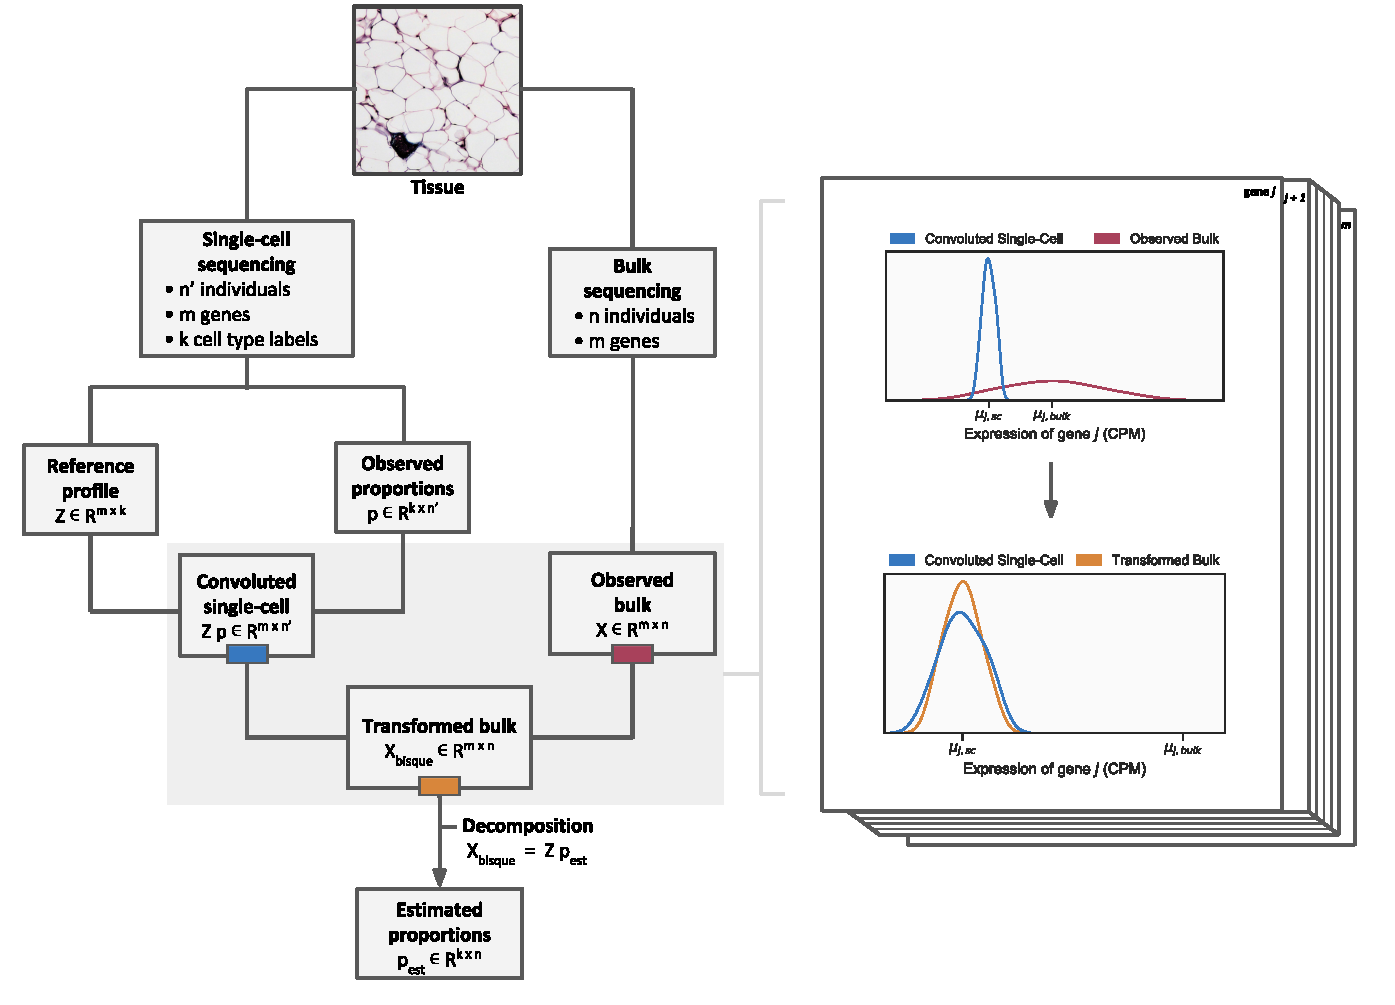
\includegraphics[width=\textwidth]{chapter2/figures/fig1.pdf}
    \caption{
            Graphical overview of the Bisque decomposition method. We integrate single-cell and bulk expression by learning gene-specific bulk transformations (pictured on right) that align the two datasets for accurate decomposition.
            }
    \label{fig:fig2.1}
\end{figure}

\subsection{Evaluation of decomposition performance in adipose tissue}
We applied our method to 106 bulk RNA-seq subcutaneous adipose tissue samples collected from both lean and obese individuals, where 6 samples have both bulk RNA-seq and snRNA-seq data available (Table \ref{table:table2.1}). Adipose tissue consists of several cell types, including adipocytes which are expected to be the most abundant population. Adipose tissue also contains structural cell types (i.e. fibroblasts and endothelial cells) and immune cells (i.e. macrophages and T cells)~\cite{Esteve_Rafols2014-ia}. These 5 cell type populations were identified from the snRNA-seq data (Figure \ref{fig:supfig2.1}a).

\begin{table}
    \scriptsize
    \centering
    \begin{tabularx}{\textwidth}{|L|L|L|L|L|p{1cm}|L|L|}
    \hline
    \rowcolor{mygray}
    \textbf{Tissue} & \textbf{Number of Samples} & \textbf{Bulk RNA-seq platform} & \textbf{snRNA-seq platform} & \textbf{snRNA-seq samples} & \textbf{Total nuclei} & \textbf{Average nuclei per individual} & \textbf{Number of cell types}  \\ \hline
    Subcutaneous adipose & 106 & Illumina NovaSeq & 10x Genomics Chromium & 6 & 10,947 & 1,824 & 5  \\ \hline
    Dorsolateral prefrontal cortex & 636 & Illumina HiSeq & 10x Genomics Chromium & 8 & 68,028 & 8,503 & 11  \\
    \hline
    \end{tabularx}
    \captionsetup{justification=raggedright,singlelinecheck=false}
    \caption{
        Summary of snRNA-seq and bulk expression datasets used for benchmarking Bisque and existing methods. 
        }
    \label{table:table2.1}
\end{table}

\begin{figure}
\centering
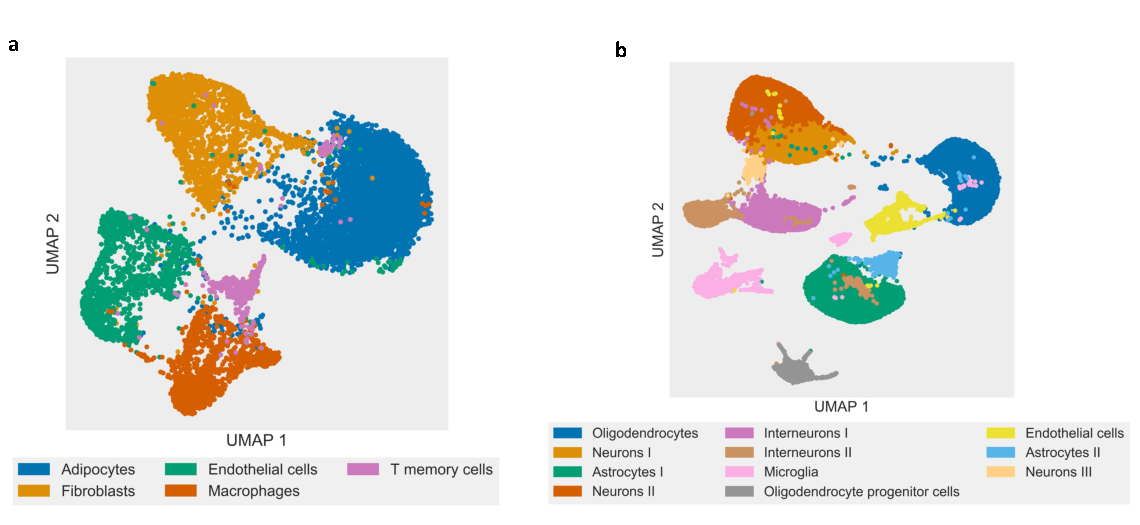
\includegraphics[width=\textwidth]{chapter2/figures/supfig1-2.pdf} 
\caption{
         Cell types quantified in snRNA-seq experiments.
         (\textbf{a}) UMAP projection of adipose snRNA-seq data with 5 identified cell type clusters labeled. (\textbf{b}) UMAP projection of cortex snRNA-seq data with 11 identified clusters.
        }
\label{fig:supfig2.1}
\end{figure}

We observed significant biases between the snRNA-seq and bulk RNA-seq data in samples that had both data available. We found that the linear relationship between the pseudo-bulk (summed snRNA-seq reads across cells) and the true bulk expression varied significantly by each gene (Figure \ref{fig:fig2.2}a). Specifically, we observed best fit lines relating these expression levels between technologies with a mean slope of roughly 0.30 and a variance in slope of 5.67. In our model, a slope of 1 would indicate no bias between technologies. We further investigated whether gene expression differences between the bulk and snRNA-seq were the same across individuals and experiments. Comparing log-ratios of RNA-seq to snRNA-seq expression levels, we found that the majority of gene biases were preserved across individuals, tissues, and experiments (R=0.75 across experiments) (Figure \ref{fig:supfig2.3}), providing evidence that technological differences drive consistent gene expression differences across bulk and snRNA-seq methods. 

\begin{figure}
\centering
\begin{multicols}{2}
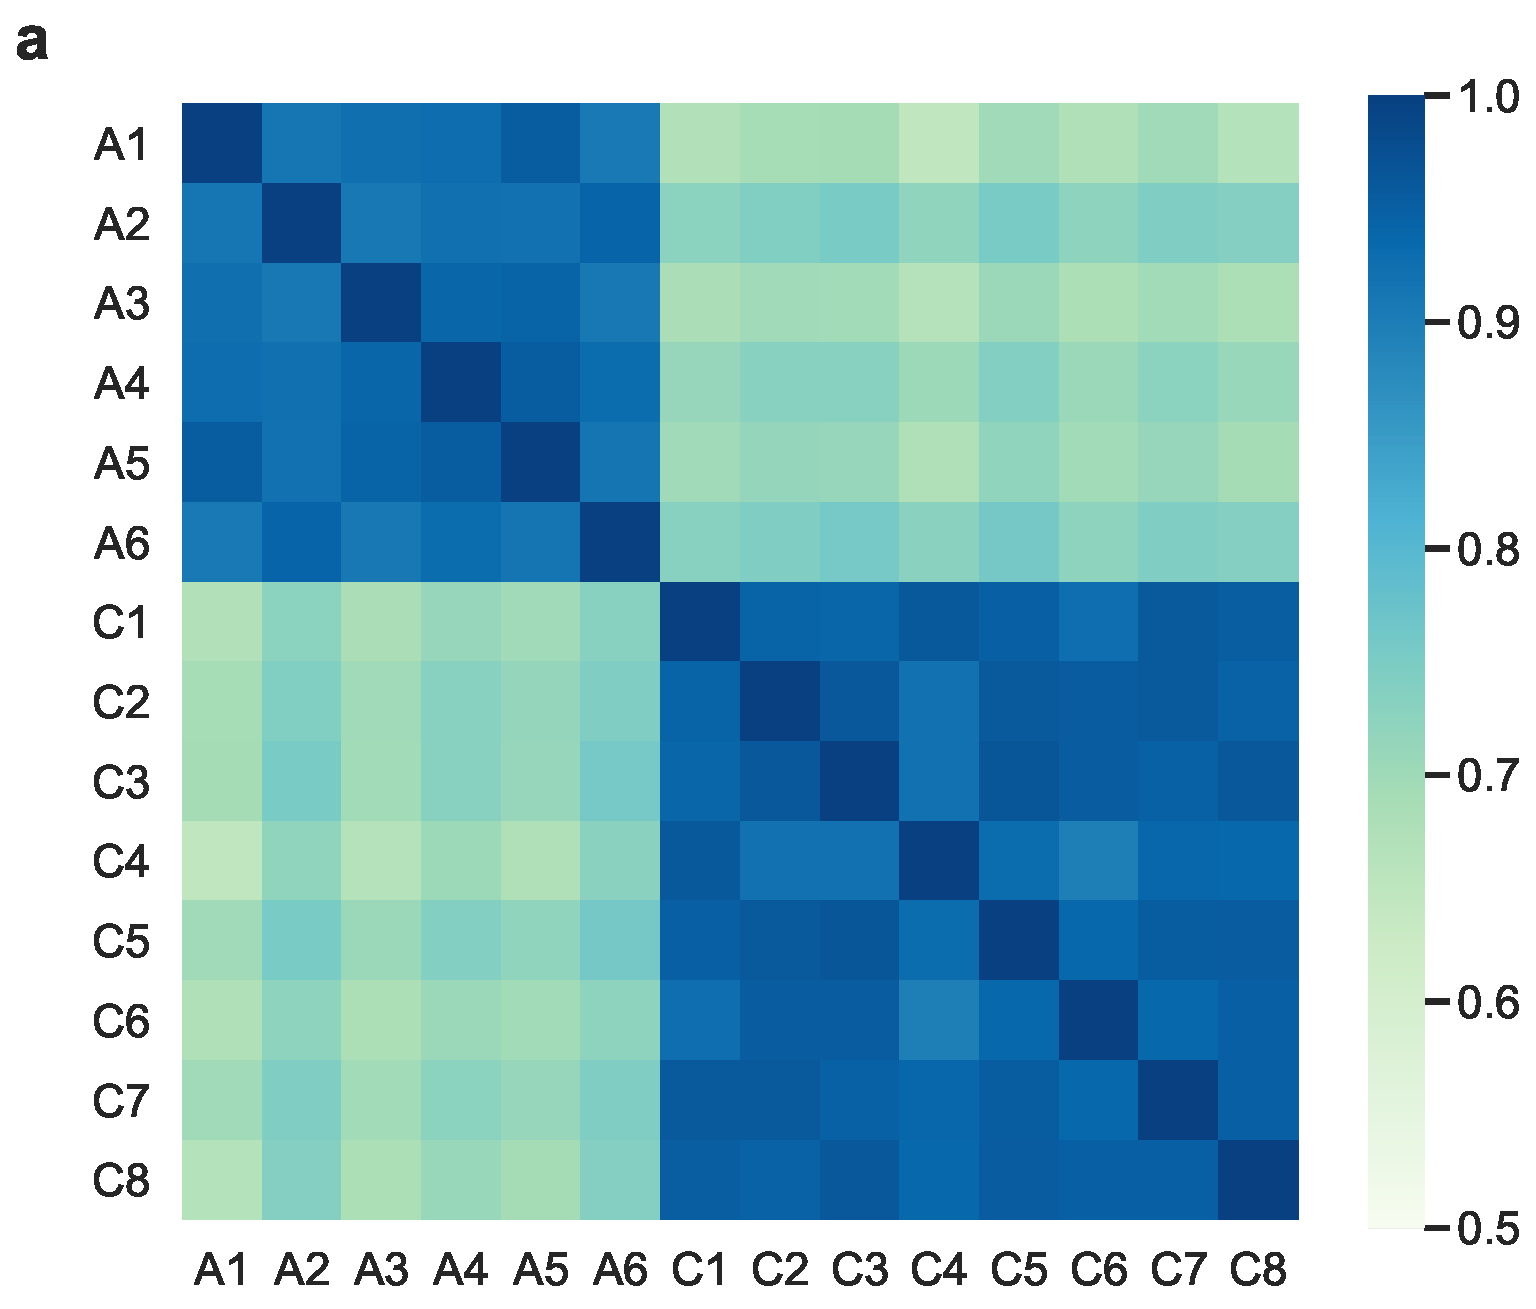
\includegraphics[scale=.3]{chapter2/figures/supfig3a.pdf}\par
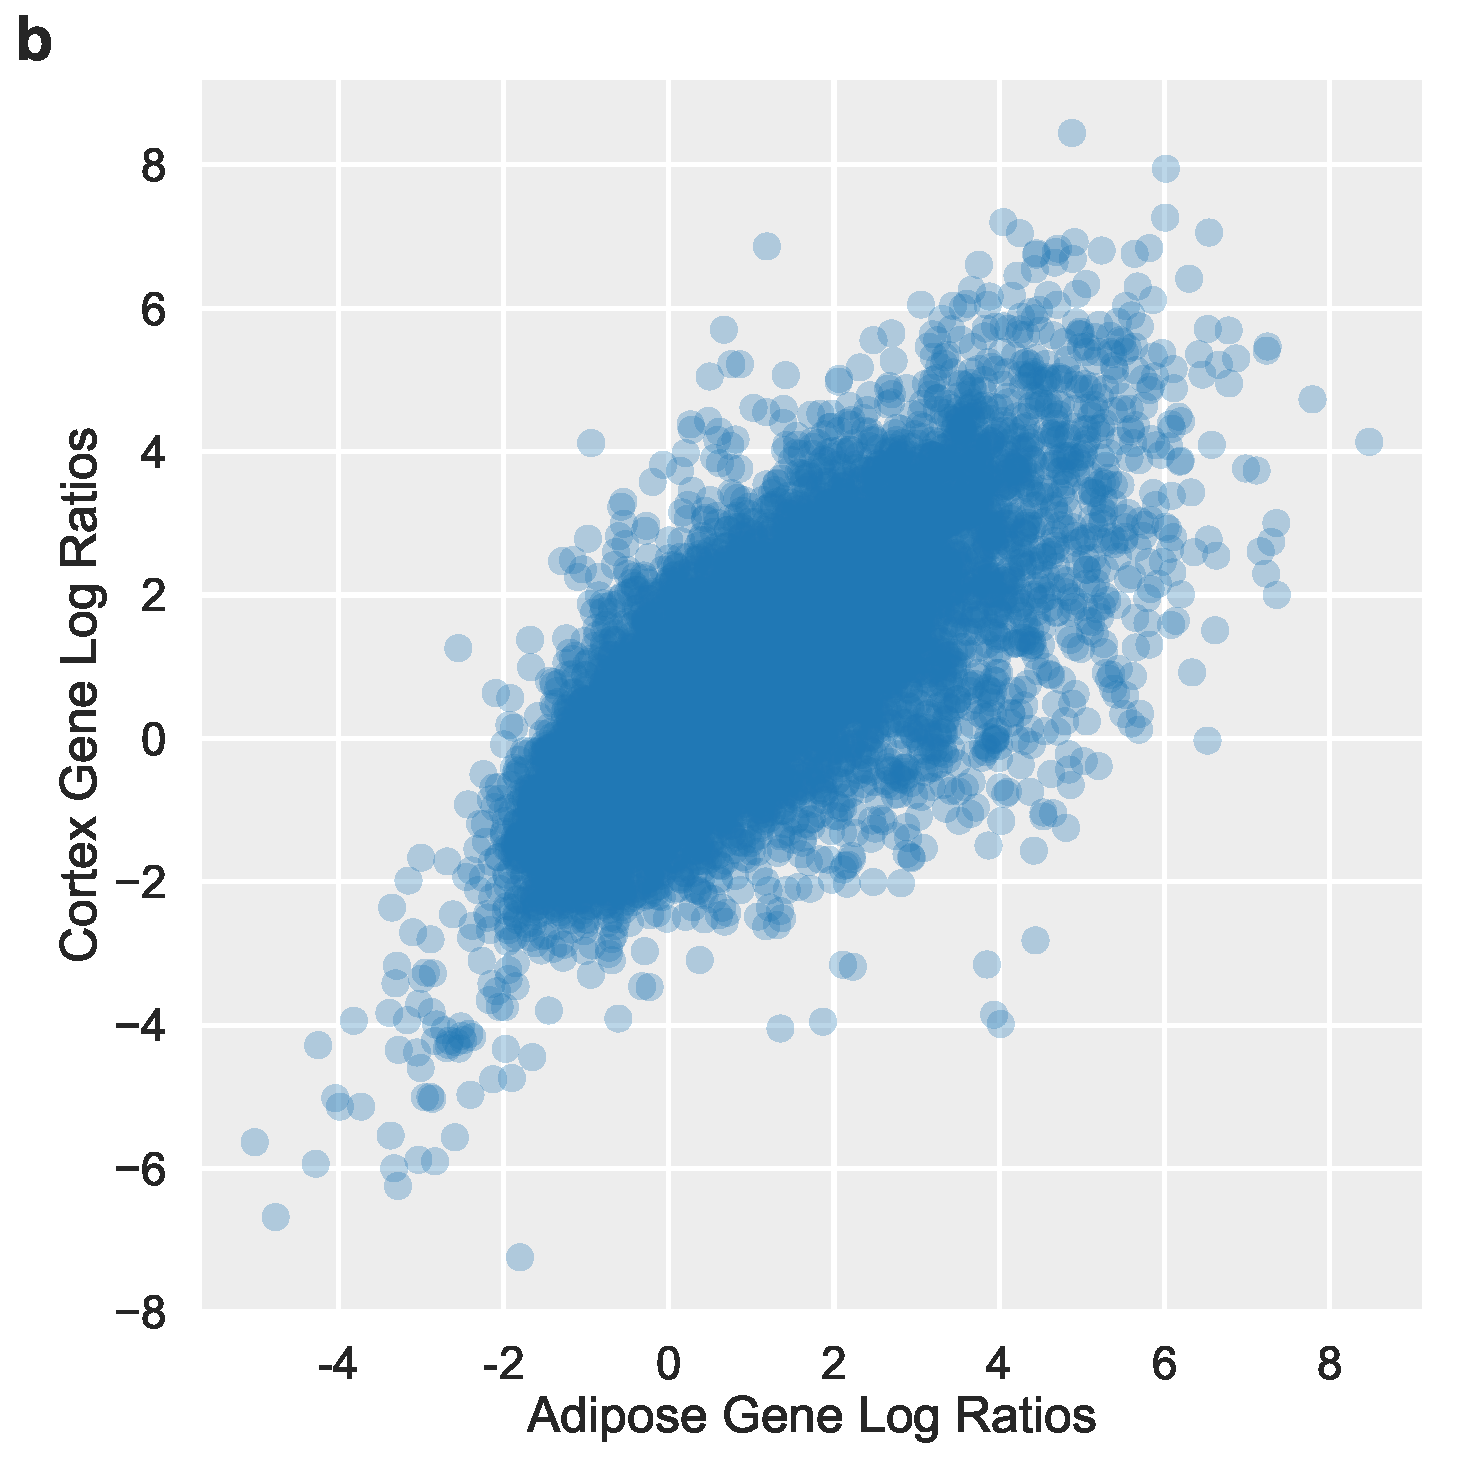
\includegraphics[scale=\figscale]{chapter2/figures/supfig3b.pdf}\par
\end{multicols}
\caption{
        Consistency of snRNA-seq to bulk RNA-seq expression log-ratios across individuals, tissues, and experiments.
        (\textbf{a}) Heatmap depicting Pearson correlation between pairs of individual’s log-ratios of snRNA-seq expression to bulk RNA-seq gene expression measured in counts per million (CPM). A sample prefix of ‘A’ indicates an individual from the adipose dataset and ‘C’ indicates an individual from the cortex dataset. Correlation is high between individuals within experiments as well as between experiments/tissues, indicating the same genes are over/under-expressed in snRNA-seq when compared to bulk RNA-seq.
        (\textbf{b}) Scatterplot of average snRNA-seq to bulk RNA-seq gene expression log-ratios across individuals in adipose dataset (x-axis) and cortex dataset (y-axis). Each point corresponds to a gene detected in both experiments, depicting the average ratio across all individuals for that tissue. The snRNA-seq to bulk RNA-seq ratios vary across genes and correlate (R=0.747) between these two experiments.
        }
\label{fig:supfig2.3}
\end{figure}

We performed simulations based on the adipose snRNA-seq data to demonstrate the effect of technology-based biases between the reference profile and bulk expression on decomposition performance. In these analyses, we benchmarked Bisque and three existing methods (MuSiC, BSEQ-sc, and CIBERSORT). Briefly, we simulated bulk expression for 6 individuals by summing the observed snRNA-seq read counts. To model discordance between the reference and bulk, we applied gene-specific linear transformations of the simulated bulk expression. For each gene, the coefficient and intercept of the linear transformation were sampled from half-normal distributions with increasing variance. In this model, a higher variance corresponds to a larger bias between sequencing experiments. While these transformations closely mirrored the Bisque decomposition model, they utilized the true snRNA-seq counts for each individual whereas Bisque learned these transformations using the reference profile generated from averaging these counts across all cells. Hence, this simulation framework introduced additional noise that Bisque does not entirely model. We evaluated decomposition performance by comparing proportion estimates to the proportions observed in the snRNA-seq data in terms of global Pearson correlation (R) and root mean squared deviation (RMSD). Due to the small number of samples, we applied leave-one-out cross-validation to predict the cell composition of each individual using the remaining snRNA-seq samples as training data for each method. In these simulations, Bisque remained robust (R $\approx$ 0.85, RMSD $\approx$ 0.07) at higher levels of simulated bias between the bulk and snRNA-seq-based reference (Figure \ref{fig:fig2.2}b).

\begin{figure}
    \centering
    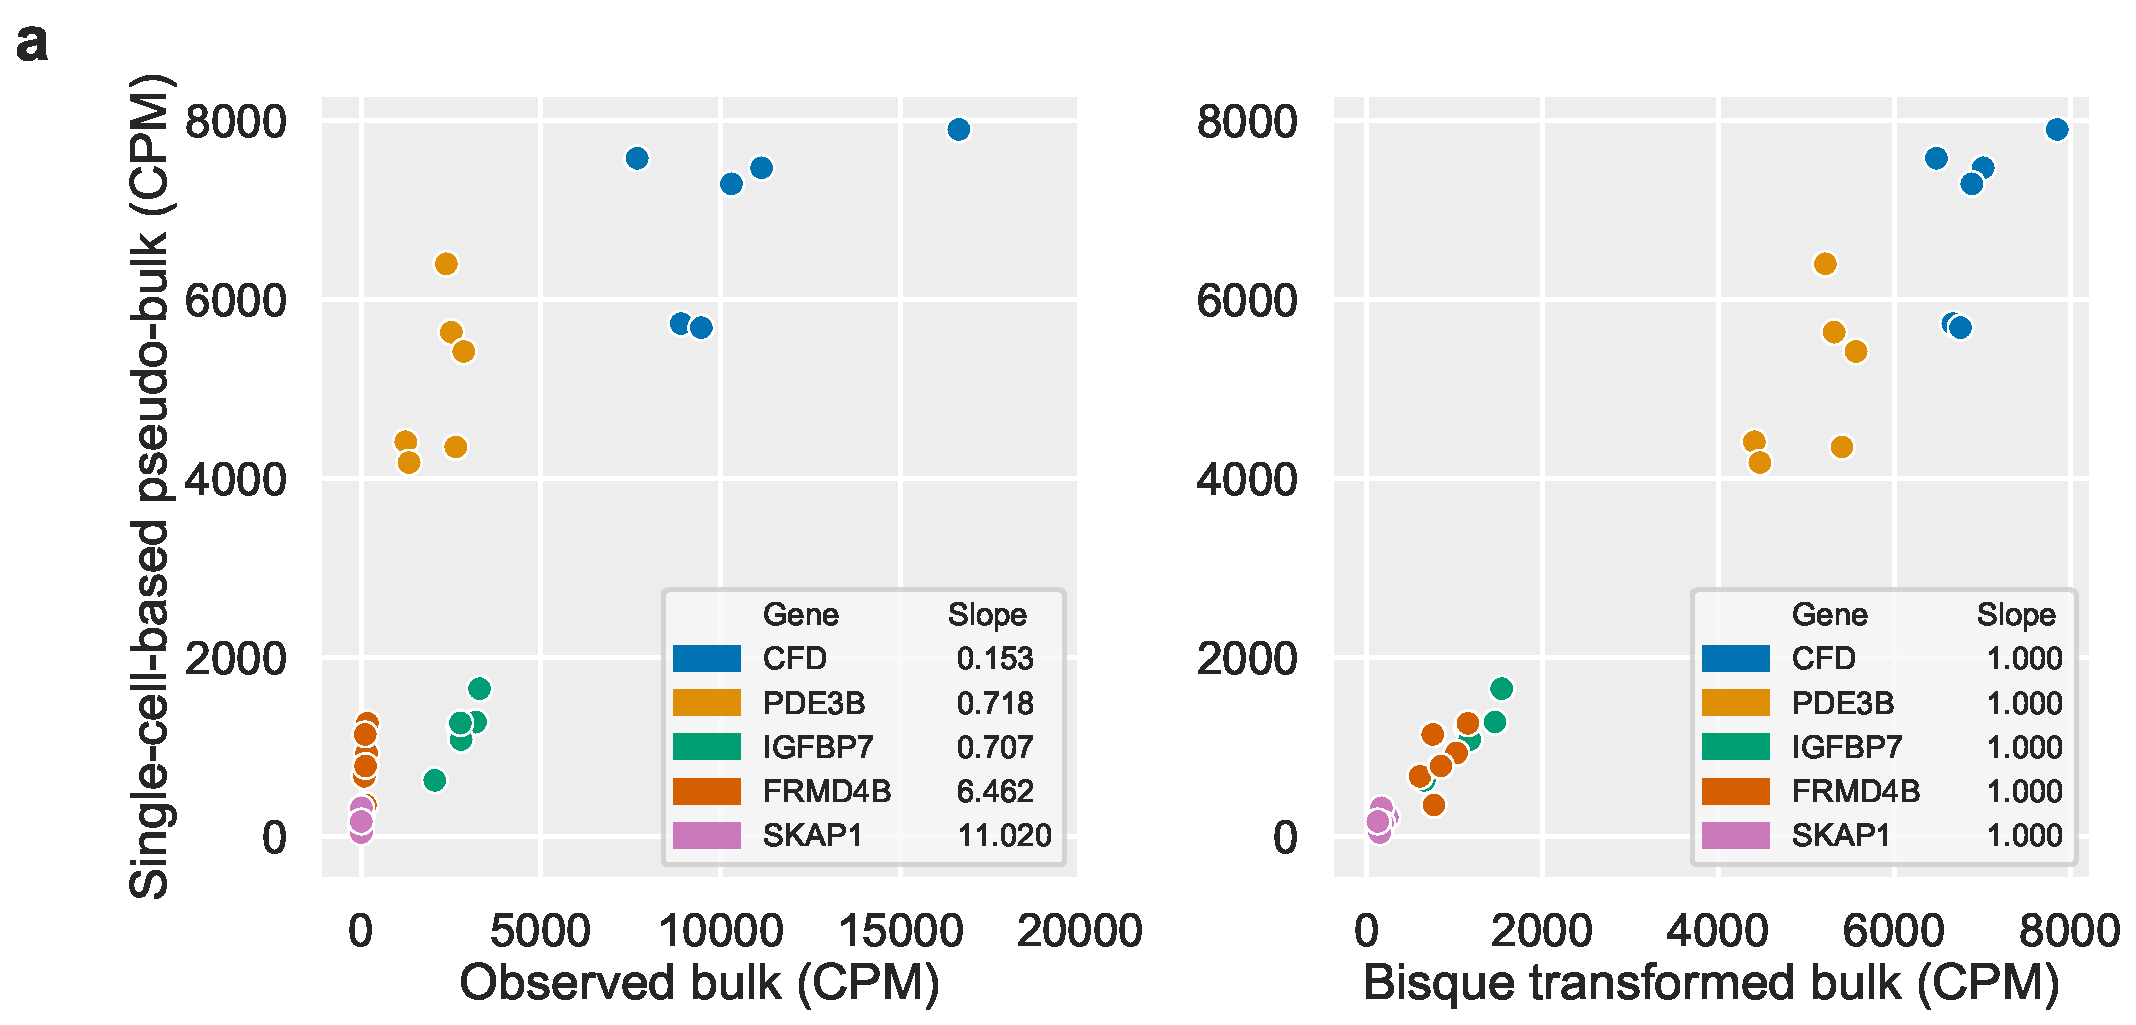
\includegraphics[scale=\figscale]{chapter2/figures/fig2a.pdf} \\[0.25in]
    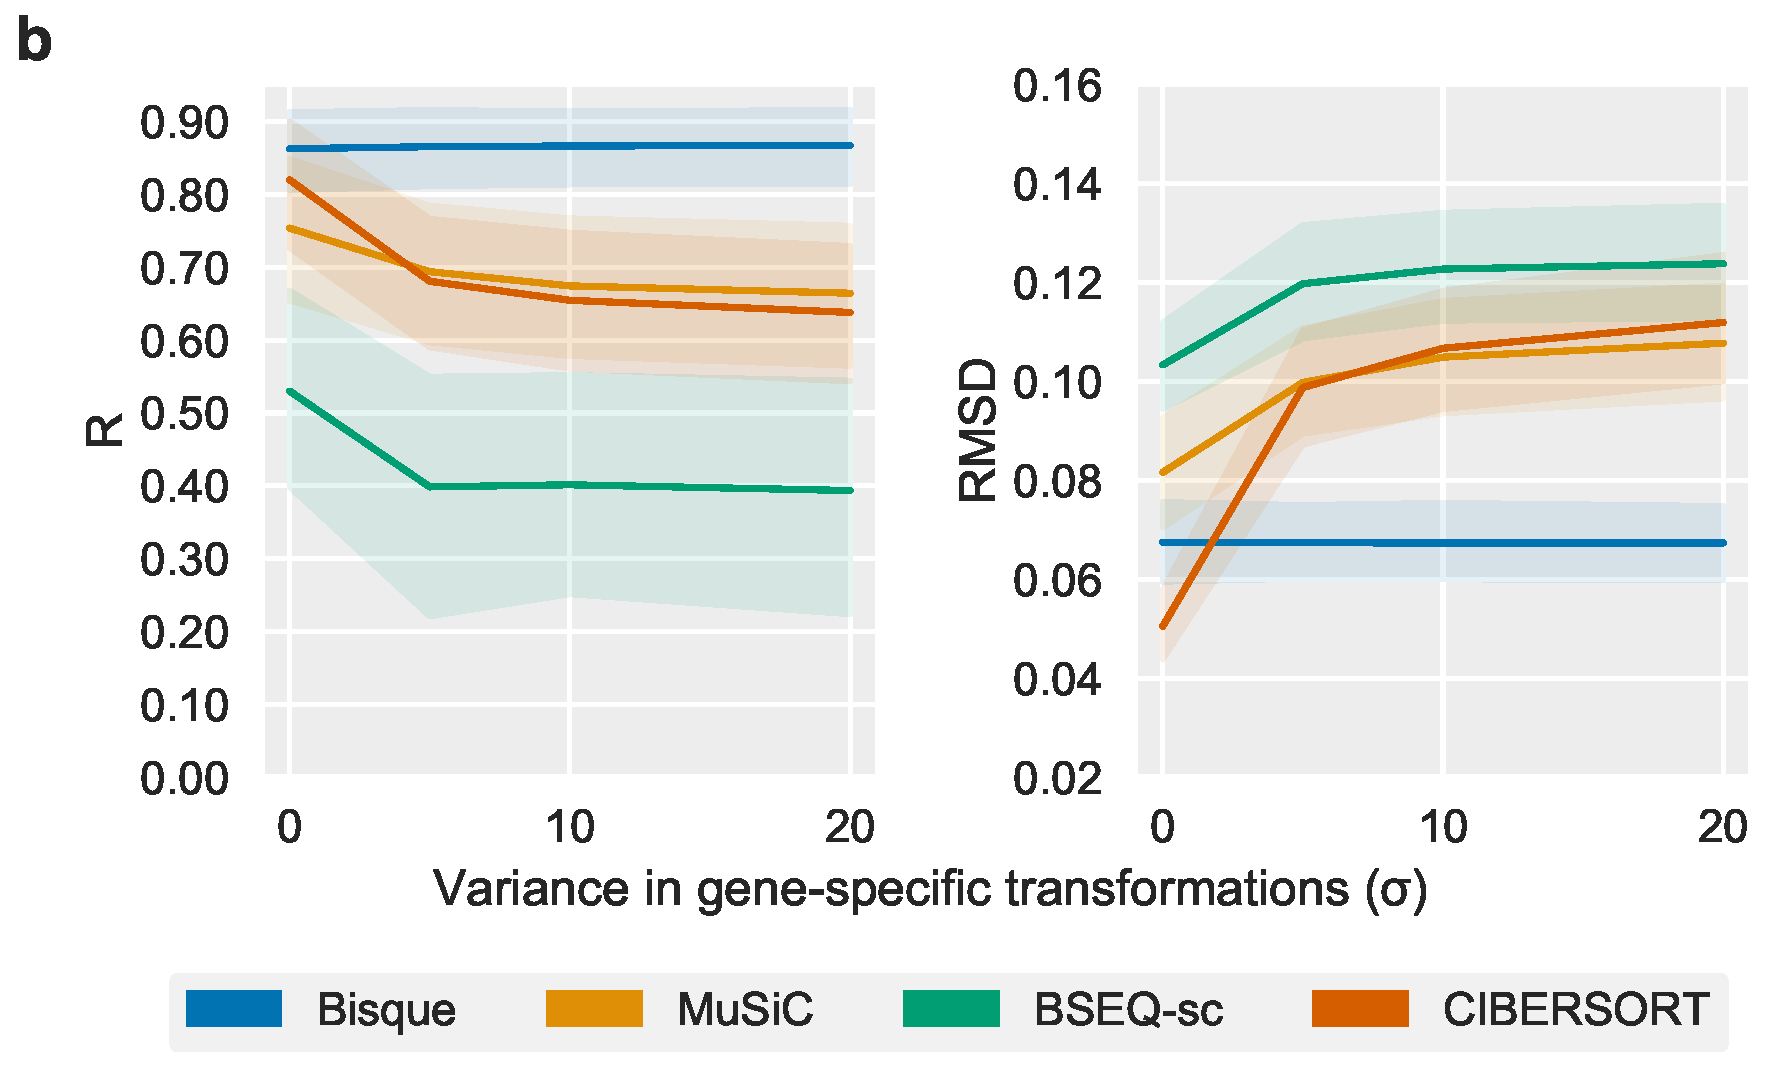
\includegraphics[scale=\figscale]{chapter2/figures/fig2b.pdf}
    \\[0.25in]
    \caption{
             The effect of discrepancies between a single-cell based reference and bulk expression on decomposition. (\textbf{a}) Observed discrepancies in real data between single-nucleus and bulk expression for selected
             marker genes (left) for six individuals. Each color corresponds to a gene. On the left, observed bulk expression on the x-axis is plotted against the pseudo-bulk expression on the y-axis, where pseudo-bulk expression is calculated by summing the single-cell based reference with cell proportions as weights. On the right, the Bisque transformation of bulk expression is on the x-axis. Bisque recovers a one-to-one relationship by transforming the bulk expression 
             for improved decomposition accuracy (right).  
             (\textbf{b}) Simulation of bulk expression for six individuals based on true adipose snRNA-seq data with increasing gene-specific differences. These differences are modeled as a linear transformation of the summed snRNA-seq counts with coefficient and intercept sampled from Half-Normal distributions with parameter as indicated on the x-axis. At $\sigma=0$, the simulated bulk is simply the sum of the observed single-cell read counts. Performance on y-axis measured in global Pearson correlation (R) (left) and root mean squared deviation (RMSD) (right). Shaded regions indicate 95\% confidence intervals based on bootstrapping with central lines indicate the mean observed value. Bisque remains robust to increasing gene-specific variation between single-cell and bulk expression levels.
            }
    \label{fig:fig2.2}
\end{figure}
	 	 	
Next, we performed this cross-validation benchmark on the observed bulk RNA-seq data for these 6 individuals and found that Bisque (R = 0.923, RMSD = 0.074) provided significantly improved global accuracy in detecting each cell type over existing methods (Table \ref{table:table2.2}). MuSiC (R = -0.111, RMSD = 0.427), BSEQ-sc (R = -0.113, RMSD = 0.432), and CIBERSORT (R = -0.131, RMSD = 0.416) severely underestimated the proportion of adipocytes (the most abundant population in adipose tissue) while overestimating the endothelial cell fraction. We also benchmarked CIBERSORTx~\cite{Newman2019-mq}, which employs a batch correction mode to account for biases in sequencing technologies. While CIBERSORTx (R = 0.687, RMSD = 0.099) outperformed existing methods, Bisque provided improved accuracy. It should be noted that cell-specific accuracy is more informative than global R and RMSD; however, these small sample sizes did not provide robust measures of within-cell-type performance in this cross-validation framework. We were able to slightly improve the number of detected cell populations by MuSiC, BSEQ-sc, and CIBERSORT when we considered only snRNA-seq reads aligning to exonic regions of the transcriptome, indicating that intronic reads introduced increasing discrepancy between snRNA-seq and bulk RNA-seq in the context of decomposition. However, given that a significant portion of the nuclear transcriptome consists of pre-mRNA, this filtering process removed over 40 percent of cells detected in the snRNA-seq data. Moreover, Bisque provided improved accuracy over existing methods using this exonic subset of the snRNA-seq data.
\begin{table}
    \scriptsize
    \centering
    \begin{tabular}{|p{3cm}|p{3cm}|p{3cm}|}
    \hline
    \rowcolor{mygray}
    \textbf{Method} & \textbf{R} & \textbf{RMSD} \\ \hline
    Bisque & \textbf{0.923 $\pm$ 0.064} & \textbf{0.074 $\pm$ 0.034} \\ \hline
    CIBERSORTx & 0.687 $\pm$ 0.450 & 0.099 $\pm$ 0.046 \\ \hline
    MuSiC & -0.111 $\pm$ 0.182 & 0.427 $\pm$ 0.058 \\ \hline
    BSEQ-sc & -0.113 $\pm$ 0.180 & 0.432 $\pm$ 0.058  \\ \hline
    CIBERSORT & -0.131 $\pm$ 0.176 & 0.416 $\pm$ 0.059  \\ \hline
    \end{tabular} 
    \captionsetup{justification=raggedright,singlelinecheck=false}
    \caption{
        Leave-one-out cross-validation in subcutaneous adipose using 6 samples with snRNA-seq and bulk RNA-seq data available. Proportions based on snRNA-seq were used as a proxy for the true proportions. Performance measured in Pearson correlation (R) and root-mean-square deviation (RMSD) across all 5 identified cell types in each sample. Reported values were averaged across the 6 samples with standard deviation indicated.
        }
    \label{table:table2.2}
\end{table}


We then applied these decomposition methods to the remaining 100 bulk samples and found that the distribution of cell proportion estimates produced by Bisque were most concordant with the expected distribution inferred from the limited number of snRNA-seq samples and previously reported proportions~\cite{Rosen2014-ae,Glastonbury_undated-kk} (Figure \ref{fig:fig2.3}a). While these benchmarks provided a measure of calibration (i.e. the ability to detect cell populations in expected ranges), they did not provide measurements of cell-specific proportion accuracy across individuals. In order to evaluate cell-specific accuracy, we replicated previously reported associations between cell proportions and measured phenotypes. Specifically, we compared cell proportion estimates from each method to body mass index (BMI) and Matsuda index, a measure of insulin resistance. We measured the significance of these association accounting for age, age-squared, sex, and relatedness.

Obesity is associated with adipocyte hypertrophy, the expansion of the volume of fat cells~\cite{Spalding2008-ey}; thus, we expected a negative association between adipocyte proportion and BMI. Bisque, MuSiC and CIBERSORTx produced adipocyte proportion estimates that replicate this behavior, while BSEQ-sc and CIBERSORT were unable to detect this cell population (Figure \ref{fig:fig2.3}b). The adipocyte proportion estimates produced by Bisque (p = 0.030) and CIBERSORTx (p = 0.001) had a significant negative association with BMI (Table \ref{table:suptable2.1a}). In addition, macrophage abundance has been shown to increase in adipose tissue with higher levels of obesity, concomitant with a state of low grade inflammation~\cite{Weisberg2003-hx}. Each method detected macrophage populations that positively associated with BMI; however, only Bisque (p $<$ 0.001), BSEQ-sc (p = 0.004) and CIBERSORTx (p = 0.049) reached significance (Table \ref{table:suptable2.1b}). 
\begin{table}
    \scriptsize
    \centering
    \begin{tabularx}{\textwidth}{|L|L|L|L|L|L|L|L|}
    \hline
    \rowcolor{mygray}
    \textbf{Method} & \textbf{Spearman Correlation} & \textbf{Spearman p-value} & \textbf{Effect Estimate} & \textbf{Effect Standard Error} & \textbf{Effect t-value} & \textbf{Effect p-value}   \\ \hline
    Bisque & -0.178 & 0.090 & -0.282 & 0.126 & -2.240 & \textbf{0.030}  \\ \hline
    MuSiC & 0.038 & 0.719 & -0.081 & 0.108 & -0.754 & 0.455  \\ \hline
    BSEQ-sc & - & - & - & - & - & -  \\ \hline
    CIBERSORT & - & - & - & - & - & - \\ \hline
    CIBERSORTx & -0.300 & \textbf{0.004} & -0.361 & 0.100 & -3.624 & \textbf{0.001} \\ \hline
    BisqueMarker & -0.227 & \textbf{0.030} & -0.304 & 0.096 & -3.154 & \textbf{0.003}  \\ \hline    
    \end{tabularx}
    \caption{Association of adipocyte proportion with BMI. A negative association was expected.}
    \label{table:suptable2.1a}
\end{table}
\begin{table}
    \scriptsize
    \centering
    \begin{tabularx}{\textwidth}{|L|L|L|L|L|L|L|L|}
    \hline
    \rowcolor{mygray}
    \textbf{Method} & \textbf{Spearman Correlation} & \textbf{Spearman p-value} & \textbf{Effect Estimate} & \textbf{Effect Standard Error} & \textbf{Effect t-value} & \textbf{Effect p-value}   \\ \hline
    Bisque & 0.389 & \textbf{$\mathbf{<}$ 0.001} & 0.460 & 0.099 & 4.671 & \textbf{$\mathbf{<}$ 0.001}  \\ \hline
    MuSiC & 0.065 & 0.540 & 0.034 & 0.110 & 0.308 & 0.760  \\ \hline
    BSEQ-sc & 0.238 & \textbf{0.022} & 0.278 & 0.092 & 3.013 & \textbf{0.004}  \\ \hline
    CIBERSORT & 0.239 & \textbf{0.022} & 0.162 & 0.102 & 1.597 & 0.118 \\ \hline
    CIBERSORTx & 0.273 & \textbf{0.009} & 0.224 & 0.102 & 2.192 & \textbf{0.034} \\ \hline
    BisqueMarker & 0.296 & \textbf{0.004} & 0.253 & 0.103 & 2.465 & \textbf{0.018}  \\ \hline    
    \end{tabularx}
    \caption{Association of macrophage proportion with BMI. A positive association was expected.}
    \label{table:suptable2.1b}
\end{table}

T cells were the least abundant cell type population identified from the snRNA-seq data, constituting around 4 percent of all sequenced nuclei. The abundance of T cells has been observed to positively correlate with insulin resistance~\cite{McLaughlin2014-gn}. Thus, we compared decomposition estimates for T cell proportions to Matsuda index. As a lower Matsuda index indicates higher insulin resistance, we expect a negative association between T cell proportion and Matsuda index. Proportion estimates produced by Bisque and CIBERSORTx followed this trend while the remaining existing methods did not identify T cells in the bulk samples (Figure \ref{fig:fig2.3}c). We found this association significant for Bisque (p $<$ 0.001) and CIBERSORTx (p = 0.047) (Table \ref{table:suptable2.1c}) after correcting for diabetes status, since Matsuda index may not be informative in these individuals~\cite{Gutch2015-db}. 

\begin{table}
    \scriptsize
    \centering
    \begin{tabularx}{\textwidth}{|L|L|L|L|L|L|L|X|}
    \hline
    \rowcolor{mygray}
    \textbf{Method} & \textbf{Spearman Correlation} & \textbf{Spearman p-value} & \textbf{Effect Estimate} & \textbf{Effect Standard Error} & \textbf{Effect t-value} & \textbf{Effect p-value}   \\ \hline
    Bisque & -0.195 & 0.075 & -0.387 & 0.116 & -3.328 &  \textbf{0.002}  \\ \hline
    MuSiC & - & - & - & - & - & -  \\ \hline
    BSEQ-sc & - & - & - & - & - & -  \\ \hline
    CIBERSORT & - & - & - & - & - & - \\ \hline
    CIBERSORTx & -0.317 & \textbf{0.003} & -0.230 & 0.111 & -2.068 & \textbf{0.046} \\ \hline
    BisqueMarker & -0.294 & \textbf{0.007} & -0.188 & 0.100 & -1.874 & 0.069  \\ \hline    
    \end{tabularx}
    \caption{Association of T cell proportion with Matusda index, a measure of insulin resistance. A negative association was expected. An additional covariate accounting for diabetes status was added to the LMM due to previously reported significant associations with Matsuda index.}
    \label{table:suptable2.1c}
\end{table}

\begin{figure}
\centering
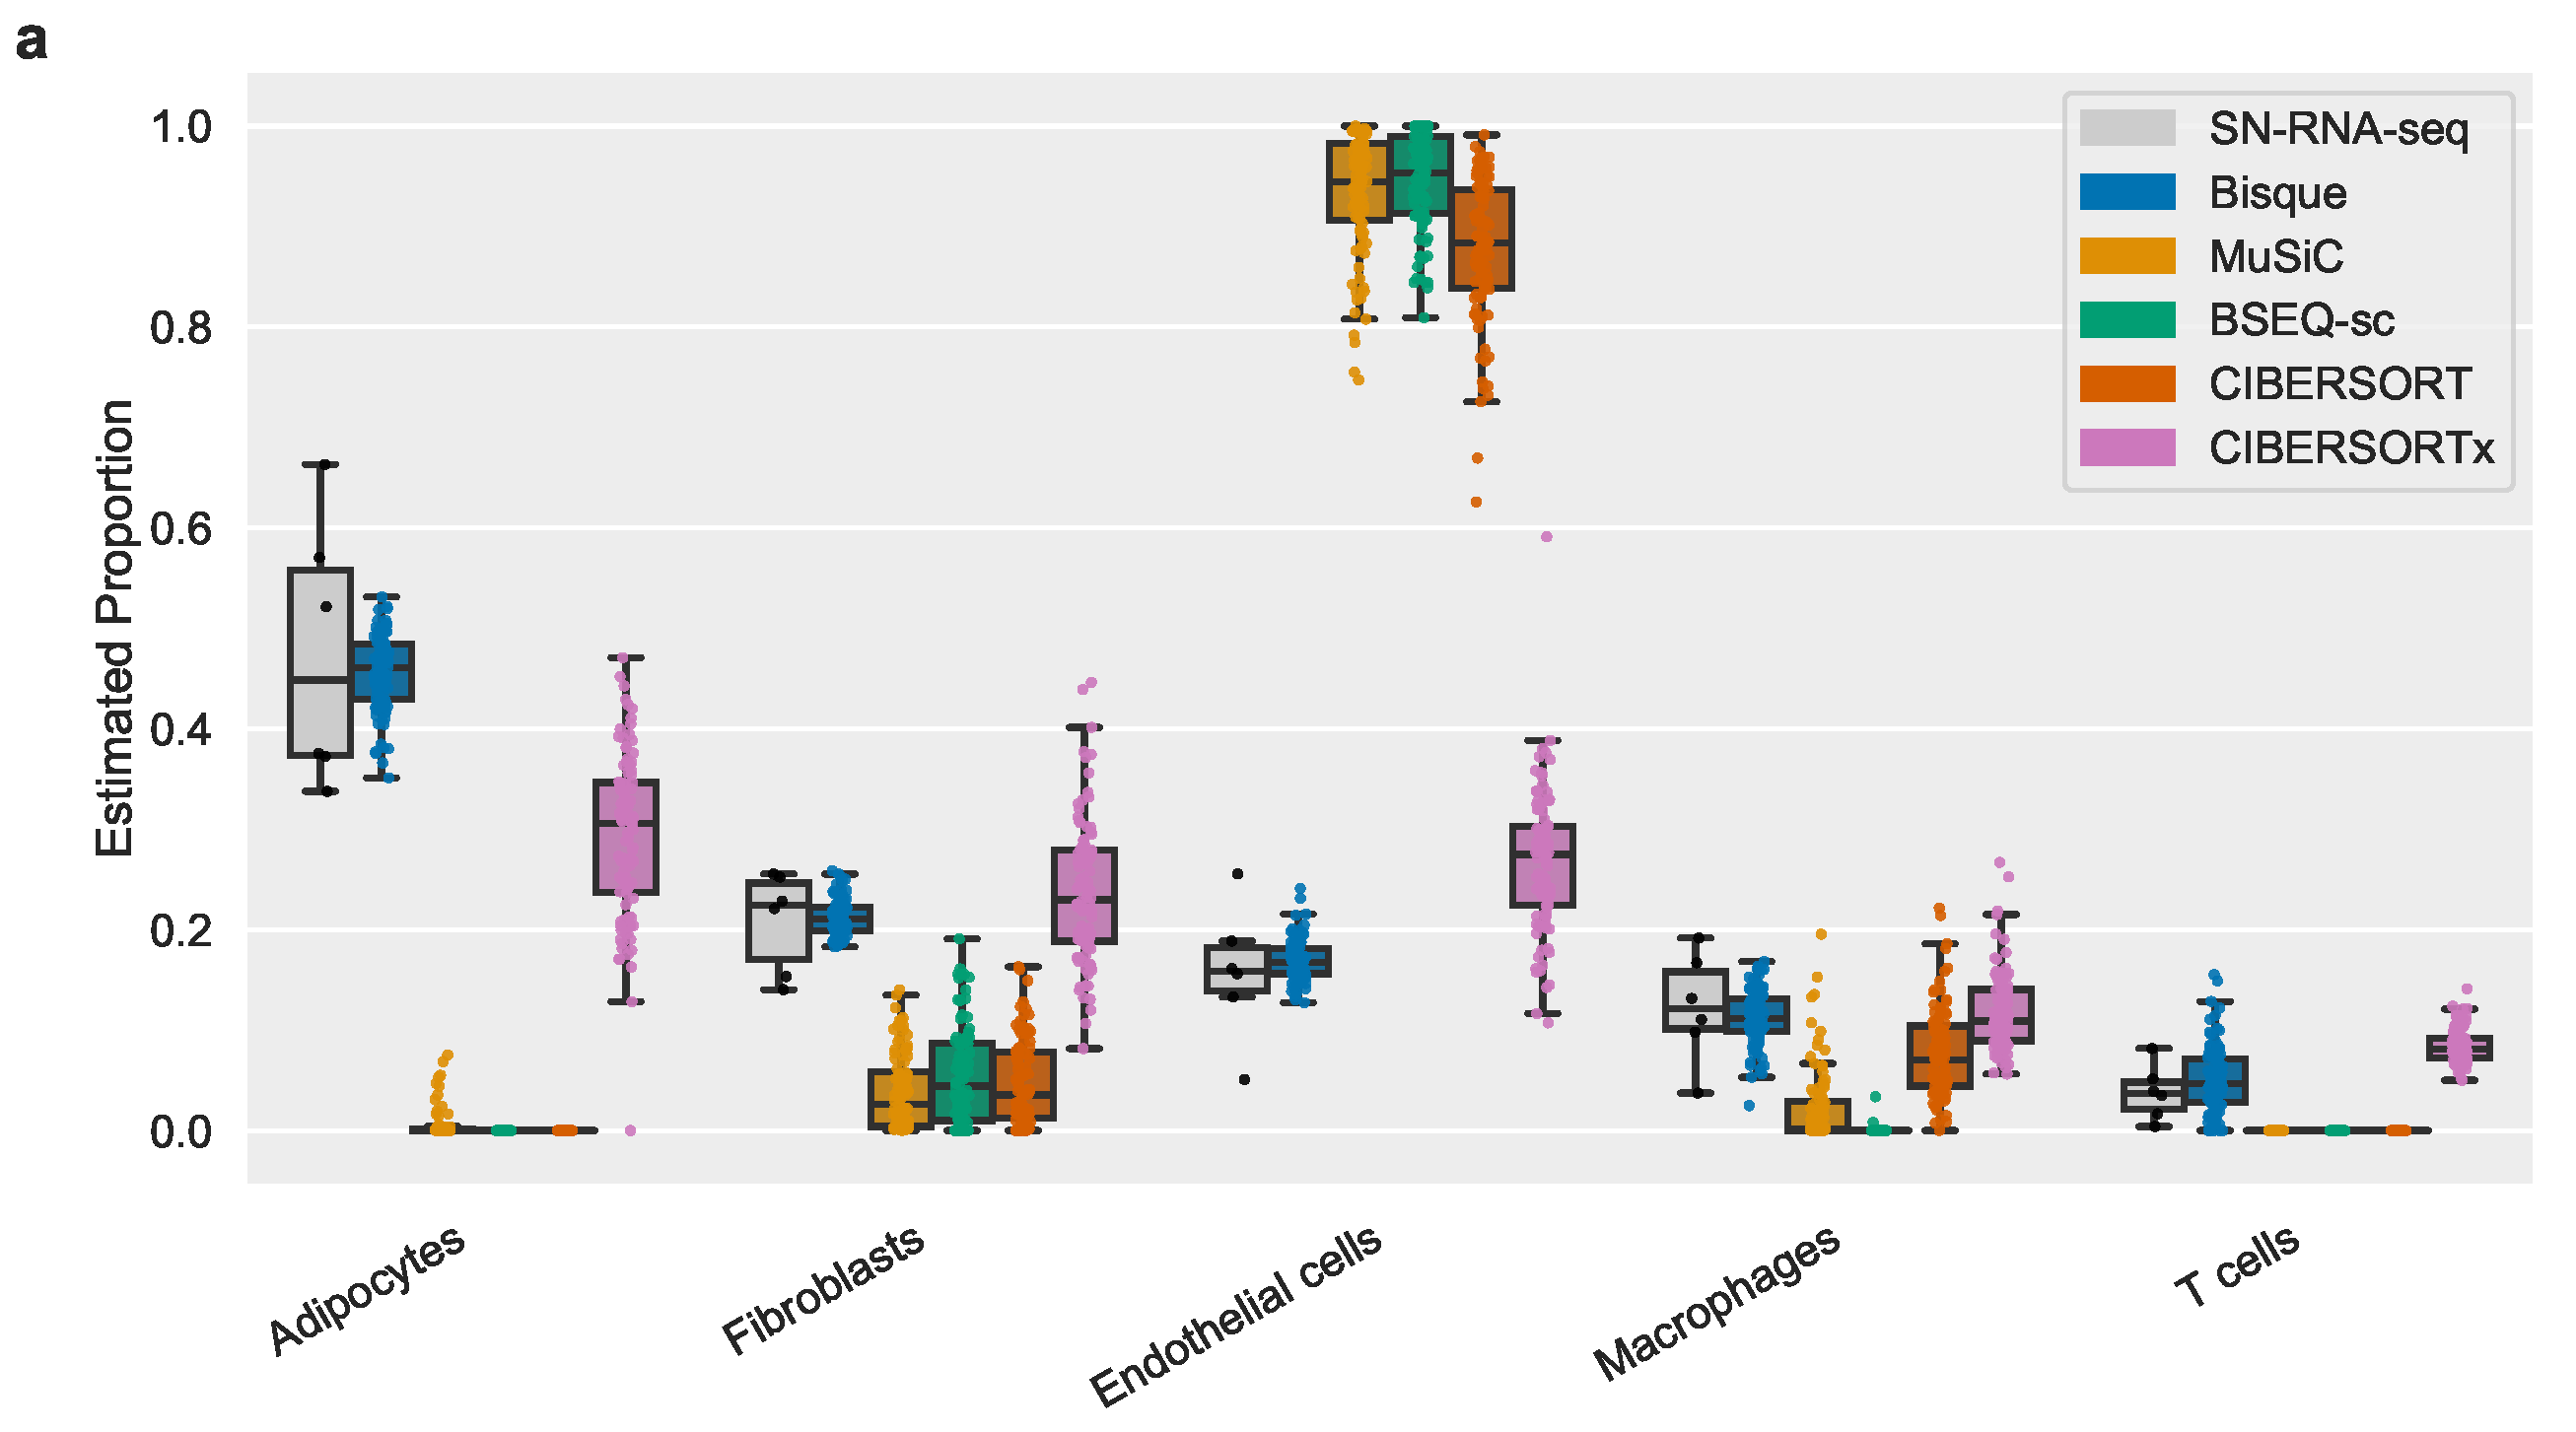
\includegraphics[scale=\figscale]{chapter2/figures/fig3a.pdf}
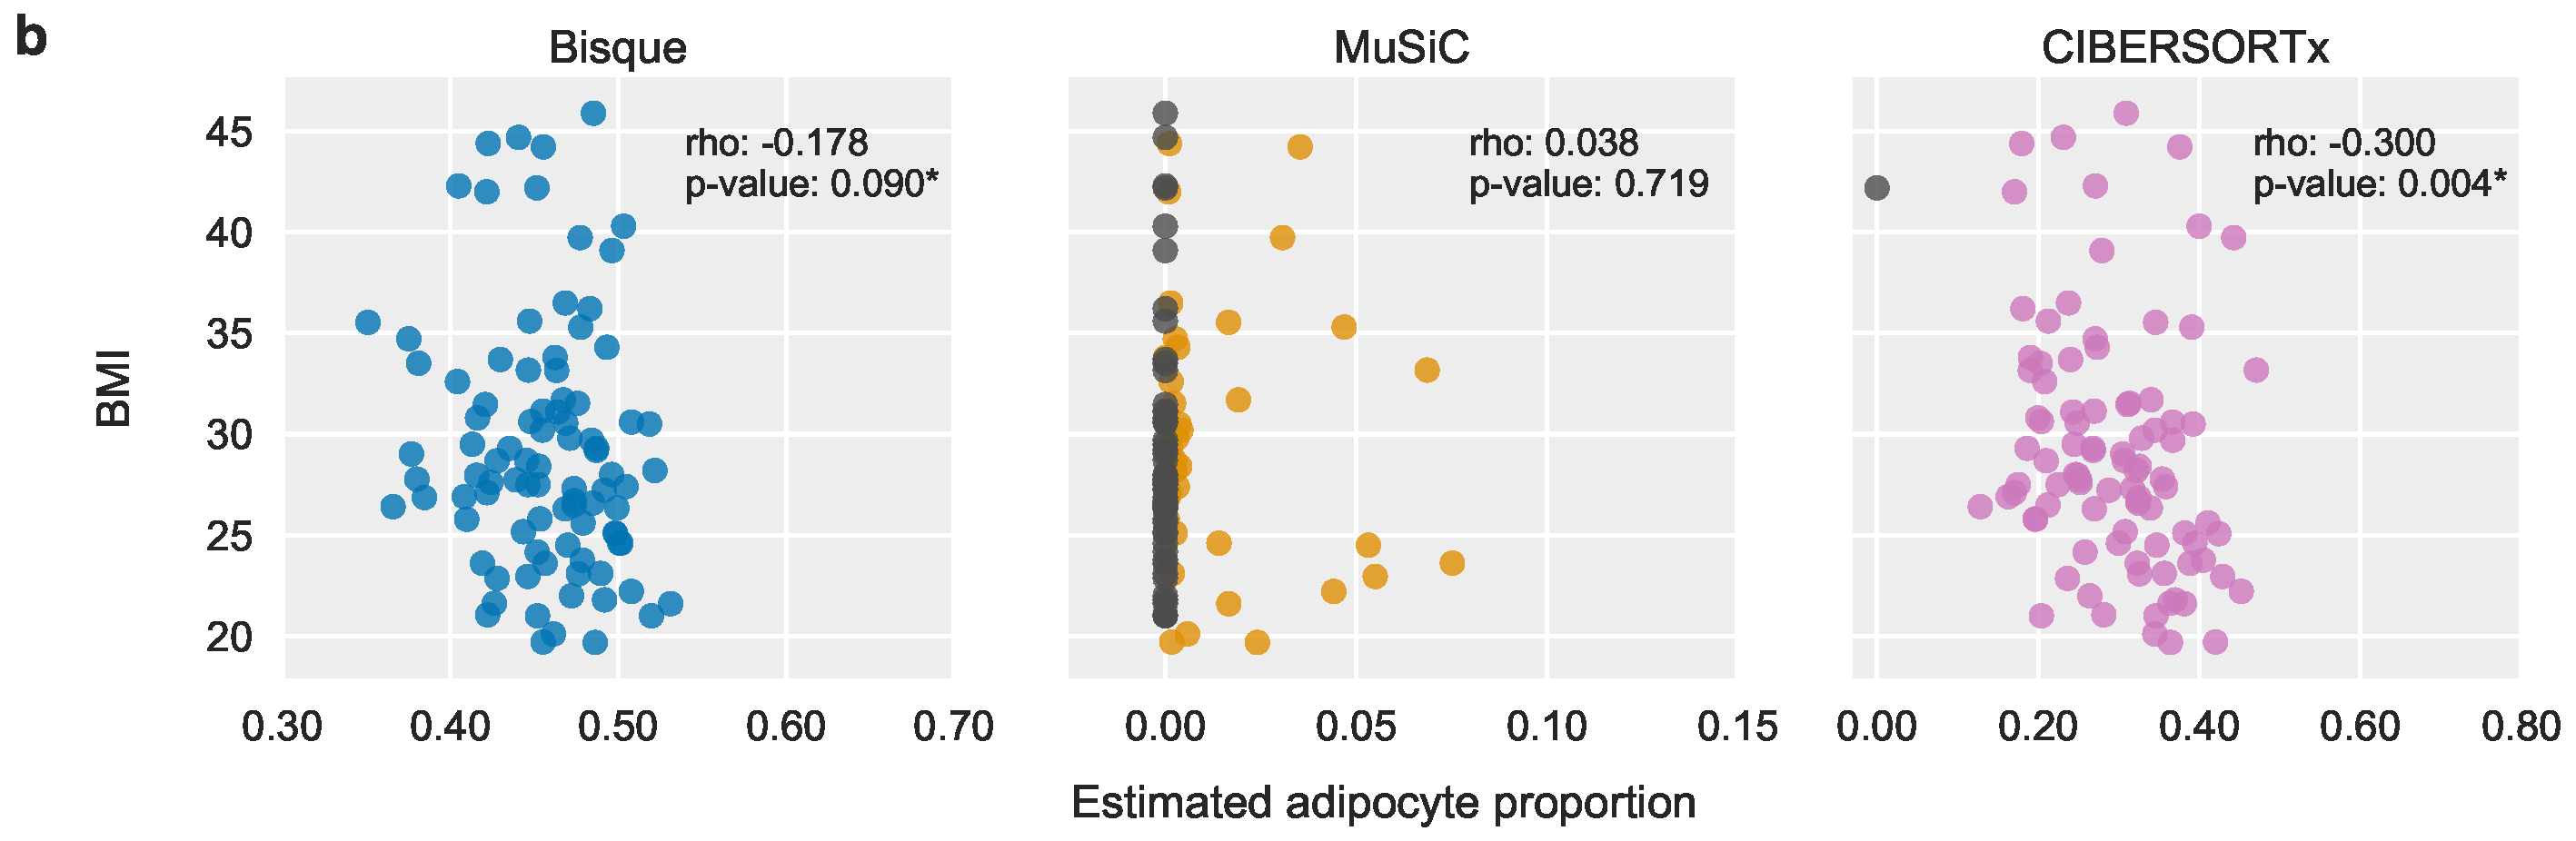
\includegraphics[scale=\figscale]{chapter2/figures/fig3b.pdf}
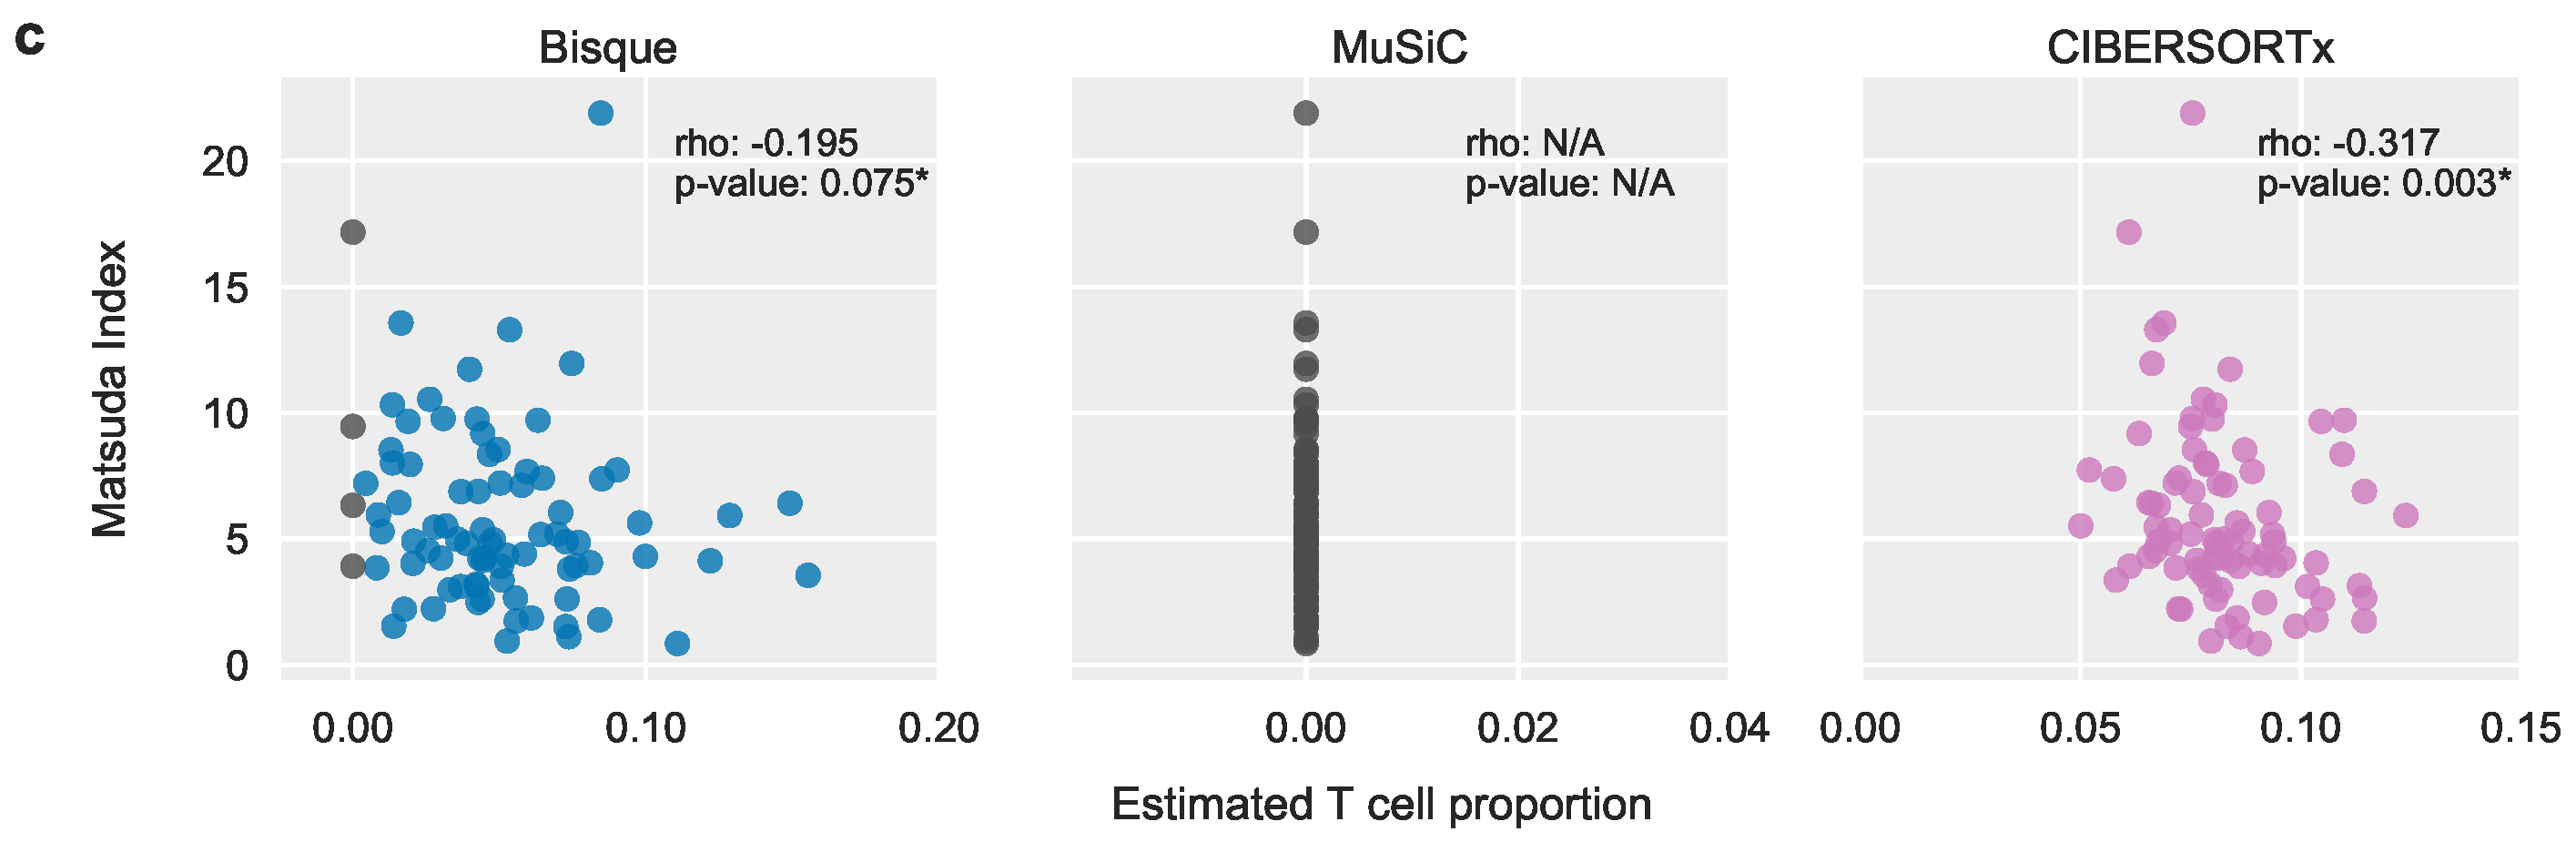
\includegraphics[scale=\figscale]{chapter2/figures/fig3c.pdf}
\caption{
         Decomposition benchmark in human subcutaneous adipose tissue.
         (\textbf{a}) Comparison of decomposition estimates from 100 individuals with estimates from 6 individuals with snRNA-seq data available. 
         (\textbf{b-c}) Scatterplots comparing decomposition estimates with measured phenotypes in 100 individuals. Reported ‘rho’ corresponds to Spearman correlation and p-values indicate the significance of these correlations, with an asterisk denoting significance after correction for covariates (sex, age, age-squared, and relatedness). CIBERSORT and BSEQ-sc are not shown since they did not detect these cell populations.
         (\textbf{b}) Adipocyte proportion has been observed to negatively correlate with BMI so we expected a negative correlation.
         (\textbf{c}) T cell proportion has previously been reported to positively correlate with insulin resistance. Matsuda index decreases with higher insulin resistance so we expected a negative correlation.
        }
\label{fig:fig2.3}
\end{figure}

\subsection{Evaluation of decomposition performance in cortex tissue}

We also benchmarked these decomposition methods using expression data collected from the dorsolateral prefrontal cortex (DLPFC). This dataset was generated by the Rush Alzheimer’s Disease (AD) Center~\cite{Mostafavi2018-ch}  and includes 636 postmortem bulk RNA-seq samples. The Religious Orders Study and Rush Memory and Aging Project were approved by an IRB of Rush University Medical Center. Both bulk RNA-seq and snRNA-seq data were collected from 8 of the individuals (Table \ref{table:table2.1}). Using the same pipeline we used to process the adipose dataset, we identified 11 clusters: 3 neuronal subtypes, 2 interneuronal subtypes, 2 astrocyte subtypes, oligodendrocytes, oligodendrocyte progenitor cells, and microglia (Figure \ref{fig:supfig2.1}b). We observed a higher overlap in marker genes for these clusters than in those identified in the adipose dataset (average of 10\% of marker genes shared between clusters in DLPFC compared to 3\% in adipose).
 	
We again applied leave-one-out cross-validation on the 8 individuals with both RNA-seq and snRNA-seq data available. In this example, randomly sampled 25\% of the nuclei in the snRNA-seq data to accommodate CIBERSORTx (which is currently web-based and restricts the size of files that can be processed). Bisque was able to detect each cell population identified from the snRNA-seq data with high global accuracy (R = 0.924, RMSD = 0.029) while MuSiC (R = -0.192, RMSD = 0.173), BSEQ-sc (R = 0.098, RMSD = 0.120), and CIBERSORT (R = -0.281, RMSD = 0.197) did not detect a number of cell populations (Table \ref{table:table2.3}). Bisque also provided higher accuracy than CIBERSORTx (R = 0.671, RMSD = 0.070). However, we found that the performance of the existing methods improved when estimates with subtypes were summed together. While each method was able to quantify major cell populations after merging subtypes, Bisque was able to distinguish between these closely related cell populations. Interestingly, we found that in both adipose and DLPFC, endothelial cell proportions were overestimated by each of the existing methods.

\begin{table}
    \scriptsize
    \centering
    \begin{tabular}{|p{3cm}|p{3cm}|p{3cm}|}
    \hline
    \rowcolor{mygray}
    \textbf{Method} & \textbf{R} & \textbf{RMSD} \\ \hline
        Bisque & \textbf{0.924 $\pm$ 0.062} & \textbf{0.029 $\pm$ 0.010} \\ \hline
        CIBERSORTx & 0.671 $\pm$ 0.153 & 0.070 $\pm$ 0.019 \\ \hline
        MuSiC & -0.192 $\pm$ 0.107 & 0.173 $\pm$ 0.013 \\ \hline
        BSEQ-sc & 0.098 $\pm$ 0.216 & 0.120 $\pm$ 0.023 \\ \hline
        CIBERSORT & -0.281 $\pm$ 0.049 & 0.197 $\pm$ 0.012 \\ \hline
    \end{tabular} 
    \captionsetup{justification=raggedright,singlelinecheck=false}
    \caption{
        Leave-one-out cross-validation in dorsolateral prefrontal cortex using 8 samples with snRNA-seq and bulk RNA-seq data available. Proportions based on snRNA-seq were used as a proxy for the true proportions. Performance measured in Pearson correlation (R) and root-mean-square deviation across all 11 identified cell types in each sample. Reported values were averaged across the 8 samples with standard deviation indicated.
        }
    \label{table:table2.3}
\end{table}
We applied these decomposition methods to the remaining 628 individuals and compared the distribution of estimates to the proportions observed in the 8 snRNA-seq samples. We found that Bisque was able to detect each cell population and produced estimates that were closest in mean to the snRNA-seq observations (Figure \ref{fig:fig2.4}a). The increased accuracy of Bisque over existing methods persisted when we merged closely related subtypes. Moreover, immunohistochemistry (IHC) analyses on 70 of these samples found similar proportions of major cell populations~\cite{Patrick_undated-vv}, confirming the relative accuracy of snRNA-seq based estimates of cell proportions. 

\begin{figure}
\centering
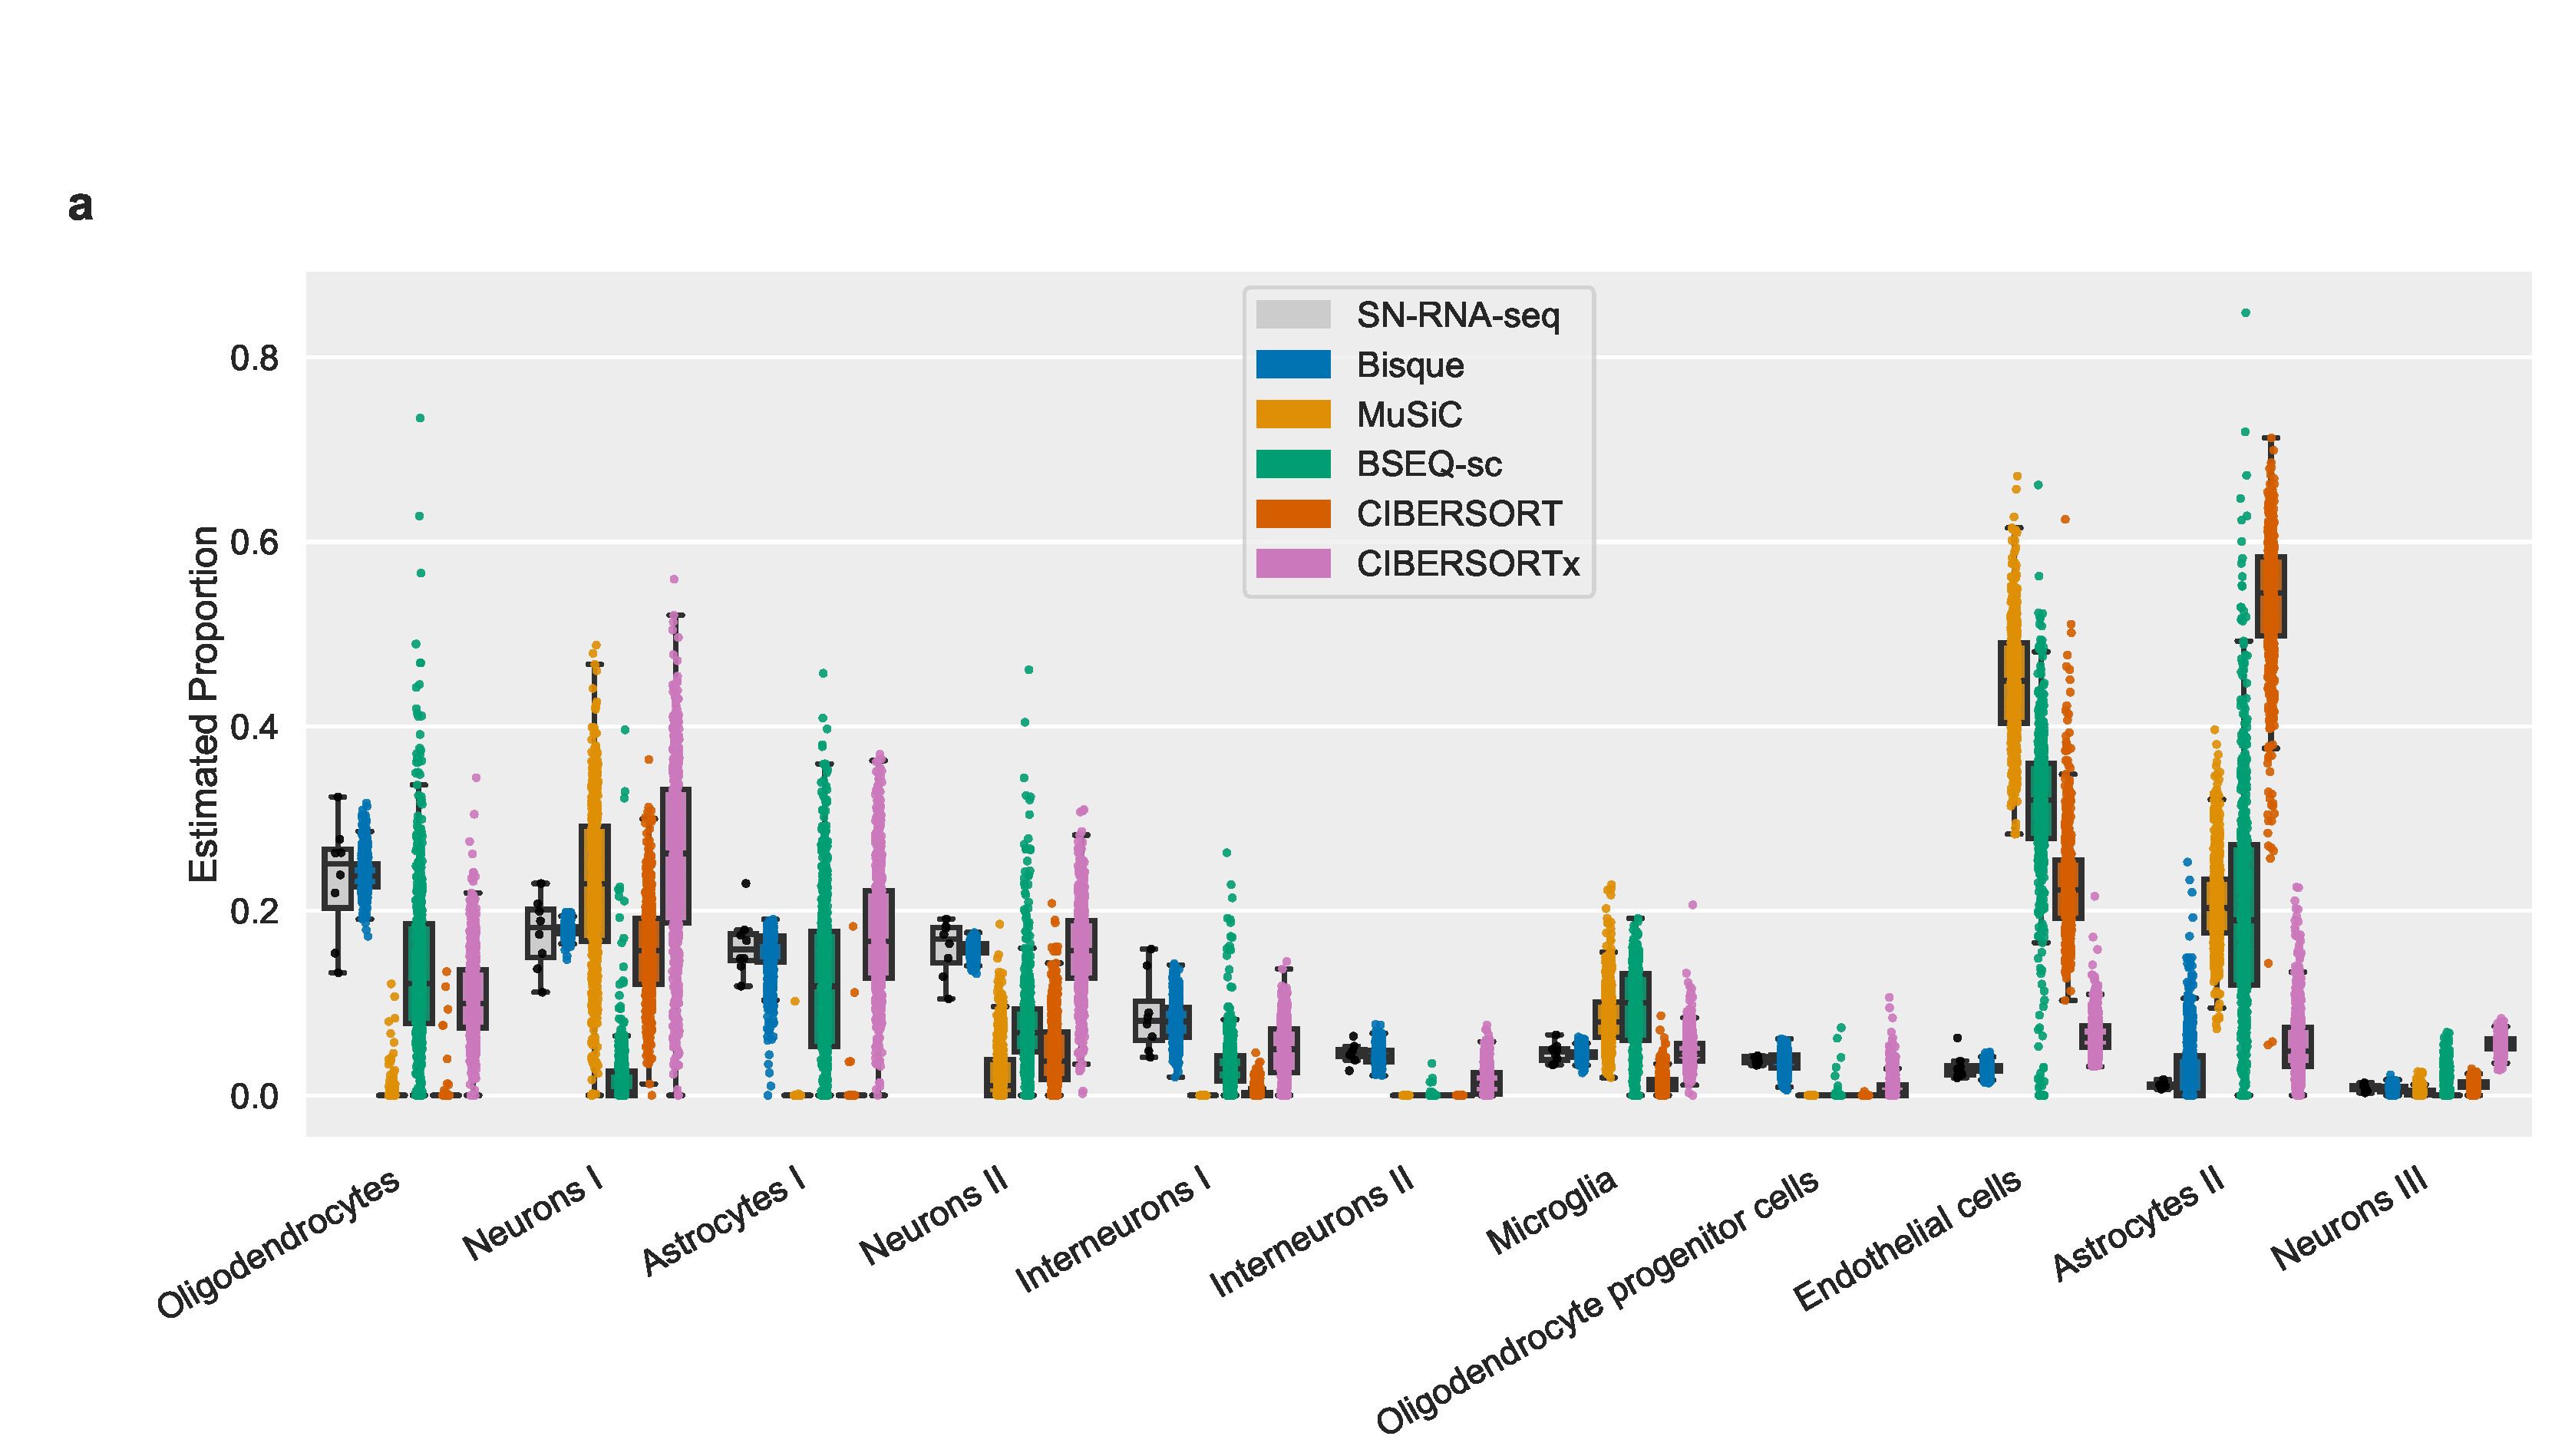
\includegraphics[scale=.24]{chapter2/figures/fig4a.pdf}
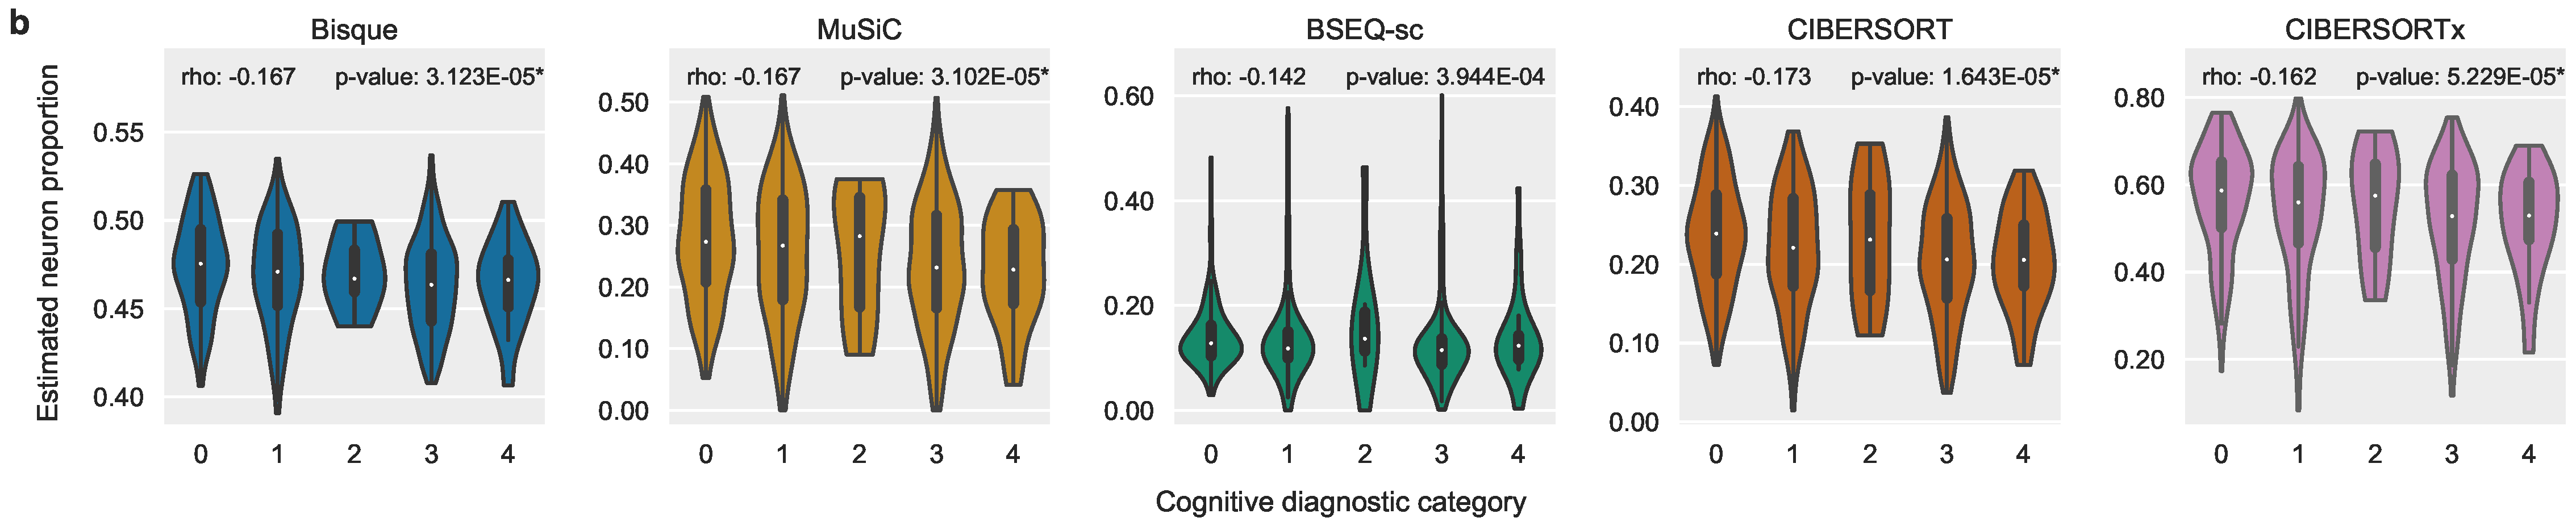
\includegraphics[width=\textwidth]{chapter2/figures/fig4b.pdf}
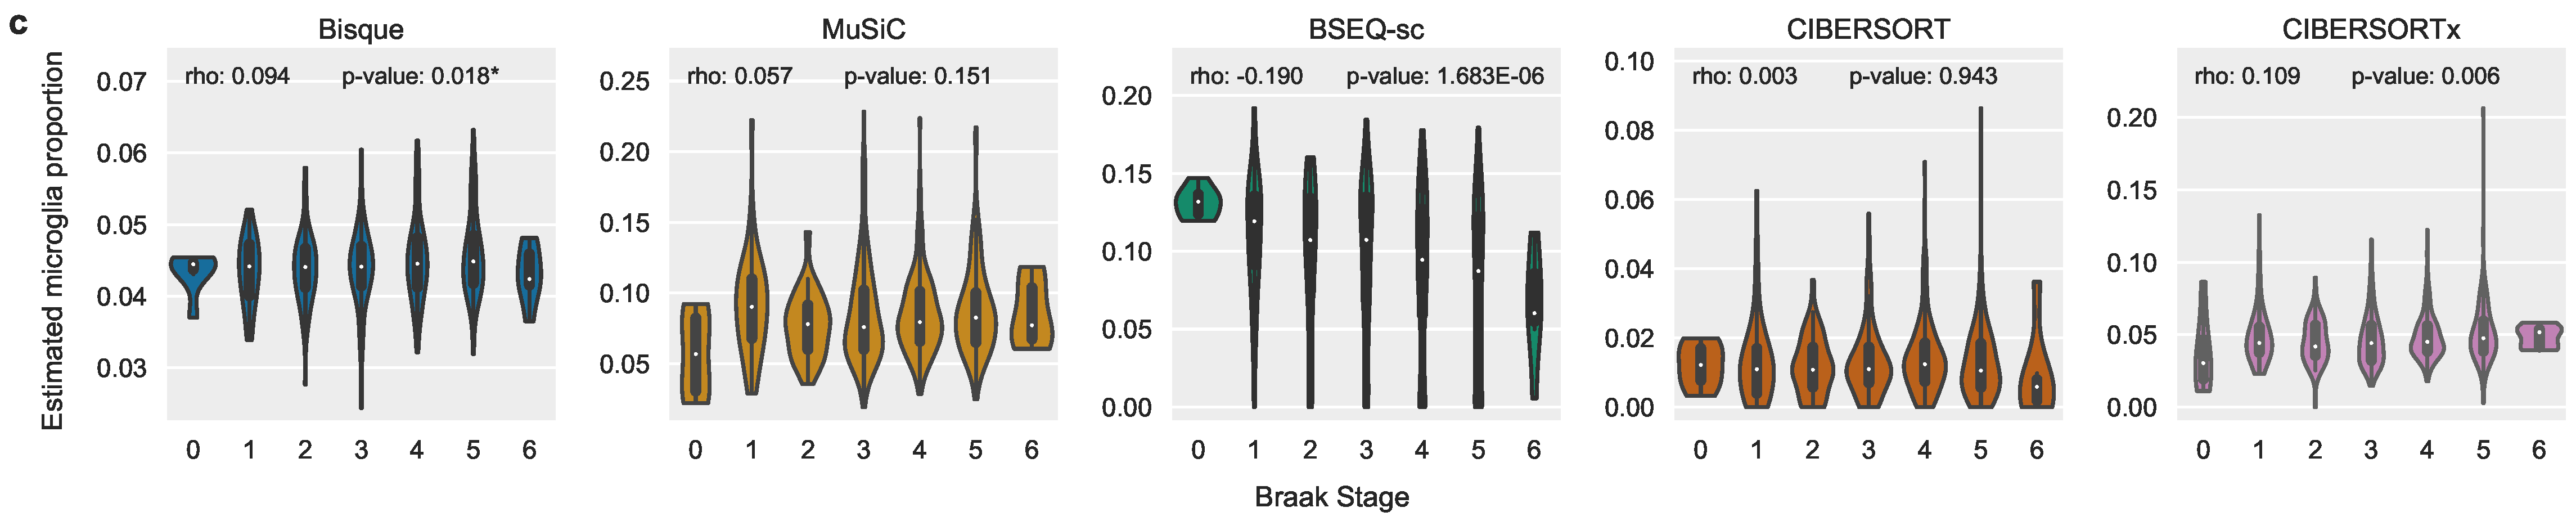
\includegraphics[width=\textwidth]{chapter2/figures/fig4c.pdf}
\caption{
    Decomposition benchmark in human dorsolateral prefrontal cortex tissue.
    (\textbf{a}) Comparison of decomposition estimates from 628 individuals with estimates from 8 individuals with snRNA-seq data available.
    (\textbf{b-c}) Violin plots depicting association of decomposition estimates aggregated into major cell types with measured phenotypes in 628 individuals. Reported ‘rho’ corresponds to Spearman correlation and p-values indicate the significance of these correlations, with an asterisk denoting both an expected effect direction and significance after correction for covariates.
    (\textbf{b}) Neuronal degeneration has been observed in patients diagnosed with Alzheimer’s disease (AD). Cognitive diagnostic category measures a physician’s diagnosis of cognitive impairment (CI), with 0 indicating no CI and 4 indicating a confident AD diagnosis. We expected a negative correlation between neuron proportion and cognitive diagnostic category.
    (\textbf{c}) Microglia proportion has been observed to positively correlate with increased severity of AD symptoms, such as neurofibrillary tangles. Braak stage provides a semiquantitative measure of tangle severity, so we expected an overall positive correlation between microglia proportion and Braak stage.
    }
\label{fig:fig2.4}
\end{figure}

\begin{table}[!ht]
    \scriptsize
    \centering
    \begin{tabularx}{\textwidth}{|L|L|L|L|L|L|L|X|}
    \hline
    \rowcolor{mygray}
    \textbf{Method} & \textbf{Spearman Correlation} & \textbf{Spearman p-value} & \textbf{Effect Estimate} & \textbf{Effect Standard Error} & \textbf{Effect t-value} & \textbf{Effect p-value}   \\ \hline
    Bisque & -0.167 & \textbf{$\mathbf{<}$ 0.001} & -0.145 & 0.039 & -3.705 &  \textbf{$\mathbf{<}$ 0.001}  \\ \hline
    MuSiC & -0.167 & \textbf{$\mathbf{<}$ 0.001} & -0.147 & 0.039 & -3.742 &  \textbf{$\mathbf{<}$ 0.001}  \\ \hline
    BSEQ-sc & -0.142 & \textbf{$\mathbf{<}$ 0.001} & -0.053 & 0.039 & -1.341 & 0.180  \\ \hline
    CIBERSORT & -0.173 & \textbf{$\mathbf{<}$ 0.001} & -0.155 & 0.039 & -3.971 & \textbf{$\mathbf{<}$ 0.001} \\ \hline
    CIBERSORTx & -0.162 & \textbf{$\mathbf{<}$ 0.001} & -0.127 & 0.039 & -3.237 & \textbf{0.001} \\ \hline
    BisqueMarker & -0.141 & \textbf{$\mathbf{<}$ 0.001} & -0.142 & 0.039 & -3.645 & \textbf{$\mathbf{<}$ 0.001}  \\ \hline    
    \end{tabularx}
    \caption{Association of neuron proportion with cognitive diagnosis category. A negative association was expected.}
    \label{table:suptable2.2a}
\end{table}
\begin{table}
    \scriptsize
    \centering
    \begin{tabularx}{\textwidth}{|L|L|L|L|L|L|L|X|}
    \hline
    \rowcolor{mygray}
    \textbf{Method} & \textbf{Spearman Correlation} & \textbf{Spearman p-value} & \textbf{Effect Estimate} & \textbf{Effect Standard Error} & \textbf{Effect t-value} & \textbf{Effect p-value}   \\ \hline
    Bisque & 0.094 & \textbf{0.018} & 0.118 & 0.037 & 3.220 &  \textbf{0.001}  \\ \hline
    MuSiC & 0.057 & 0.151 & 0.019 & 0.037 & 0.509 & 0.611  \\ \hline
    BSEQ-sc & -0.190 & $<$ 0.001 & -0.166 & 0.037 & -4.525 & $<$ 0.001  \\ \hline
    CIBERSORT & 0.003 & 0.943 & -0.005 & 0.037 & -0.137 & 0.891 \\ \hline
    CIBERSORTx & 0.109 & \textbf{0.006} & 0.056 & 0.037 & 1.517 & 0.130 \\ \hline
    BisqueMarker & 0.092 & \textbf{0.021} & 0.054 & 0.037 & 1.444 & 0.149  \\ \hline    
    \end{tabularx}
    \caption{Association of microglia proportion with Braak stage, a measure of neurofibrillary tangles. A positive association was expected.}
    \label{table:suptable2.2b}
\end{table}

Again, to determine cell-specific decomposition accuracy, we replicated known associations between cell type proportions and measured phenotypes in the 628 individuals. For these analyses, we compared cell proportion estimates to each individual’s Braak stage and physician cognitive diagnostic category at time of death. Braak stage is a semiquantitative measure of neurofibrillary tangles, ranging in value from 0 to 5 with increasing severity. The cognitive diagnostic category provides a semiquantitative measure of dementia severity, where a code of 1 indicates no cognitive impairment and 5 indicates a confident diagnosis of AD by physicians.  We determined the significance of these associations based on t-values estimated by a linear regression model that accounted for age, age-squared, and sex. 

Neuronal death is a hallmark symptom of AD~\cite{Yankner1996-lk}. Therefore, we expected to find a negative association between cognitive diagnosis and neuron proportion. We found that each decomposition method provides estimates of total neuron proportion that tend to decrease with cognitive diagnostic category (Figure \ref{fig:fig2.4}b). Each method generates proportions with negative association with cognitive diagnosis. Each method, excluding BSEQ-sc, reached significance in this model (p $\leq$ 0.003 for each method) (Table \ref{table:suptable2.2a}). As another example, we compared each individual’s Braak stage to their estimated proportion of microglia, a relatively small cell population that constituted roughly 5 percent of the sequenced nuclei. Microglia activation has been observed to increase with AD severity~\cite{Hansen2018-jj}. We used Braak stage as a proxy for AD severity and expected a positive association between microglia proportion and Braak stage. Bisque and MuSiC provided estimates that follow this expected trend (Figure \ref{fig:fig2.4}c). Only Bisque produced estimates with a significant positive association (p = 0.001) (Table \ref{table:suptable2.2b}). Interestingly, we observe a decrease in microglia proportions estimated by Bisque in Braak stage 6 individuals which has been previously observed in AD patients~\cite{Navarro2018-ti}.



\subsection{Runtime comparisons of reference-based decomposition methods}

Given the large amounts of transcriptomic data that are becoming available, we also benchmarked these decomposition methods in terms of runtime. In the subcutaneous adipose dataset, which included 100 bulk RNA-seq samples and 6 snRNA-seq samples with about 1,800 nuclei sequenced per individual, Bisque was able to estimate cell proportions efficiently compared to existing methods. Bisque (1 second) and MuSiC (1 second) provided decomposition estimates faster than BSEQ-sc (26 seconds), CIBERSORT (27 seconds), and CIBERSORTx (389 seconds) (Figure \ref{fig:fig2.5}a).  Bisque also provided improved efficiency in processing the reduced DLPFC dataset, which included 628 bulk RNA-seq samples and 8 snRNA-seq samples with around 2,125 nuclei per individual. Bisque (4 seconds) and MuSiC (10 seconds) estimated cell proportions relatively quickly compared to BSEQ-sc (273 seconds), CIBERSORT (298 seconds), and CIBERSORTx (6,566 seconds) (Figure \ref{fig:fig2.5}b).

\begin{figure}
\centering
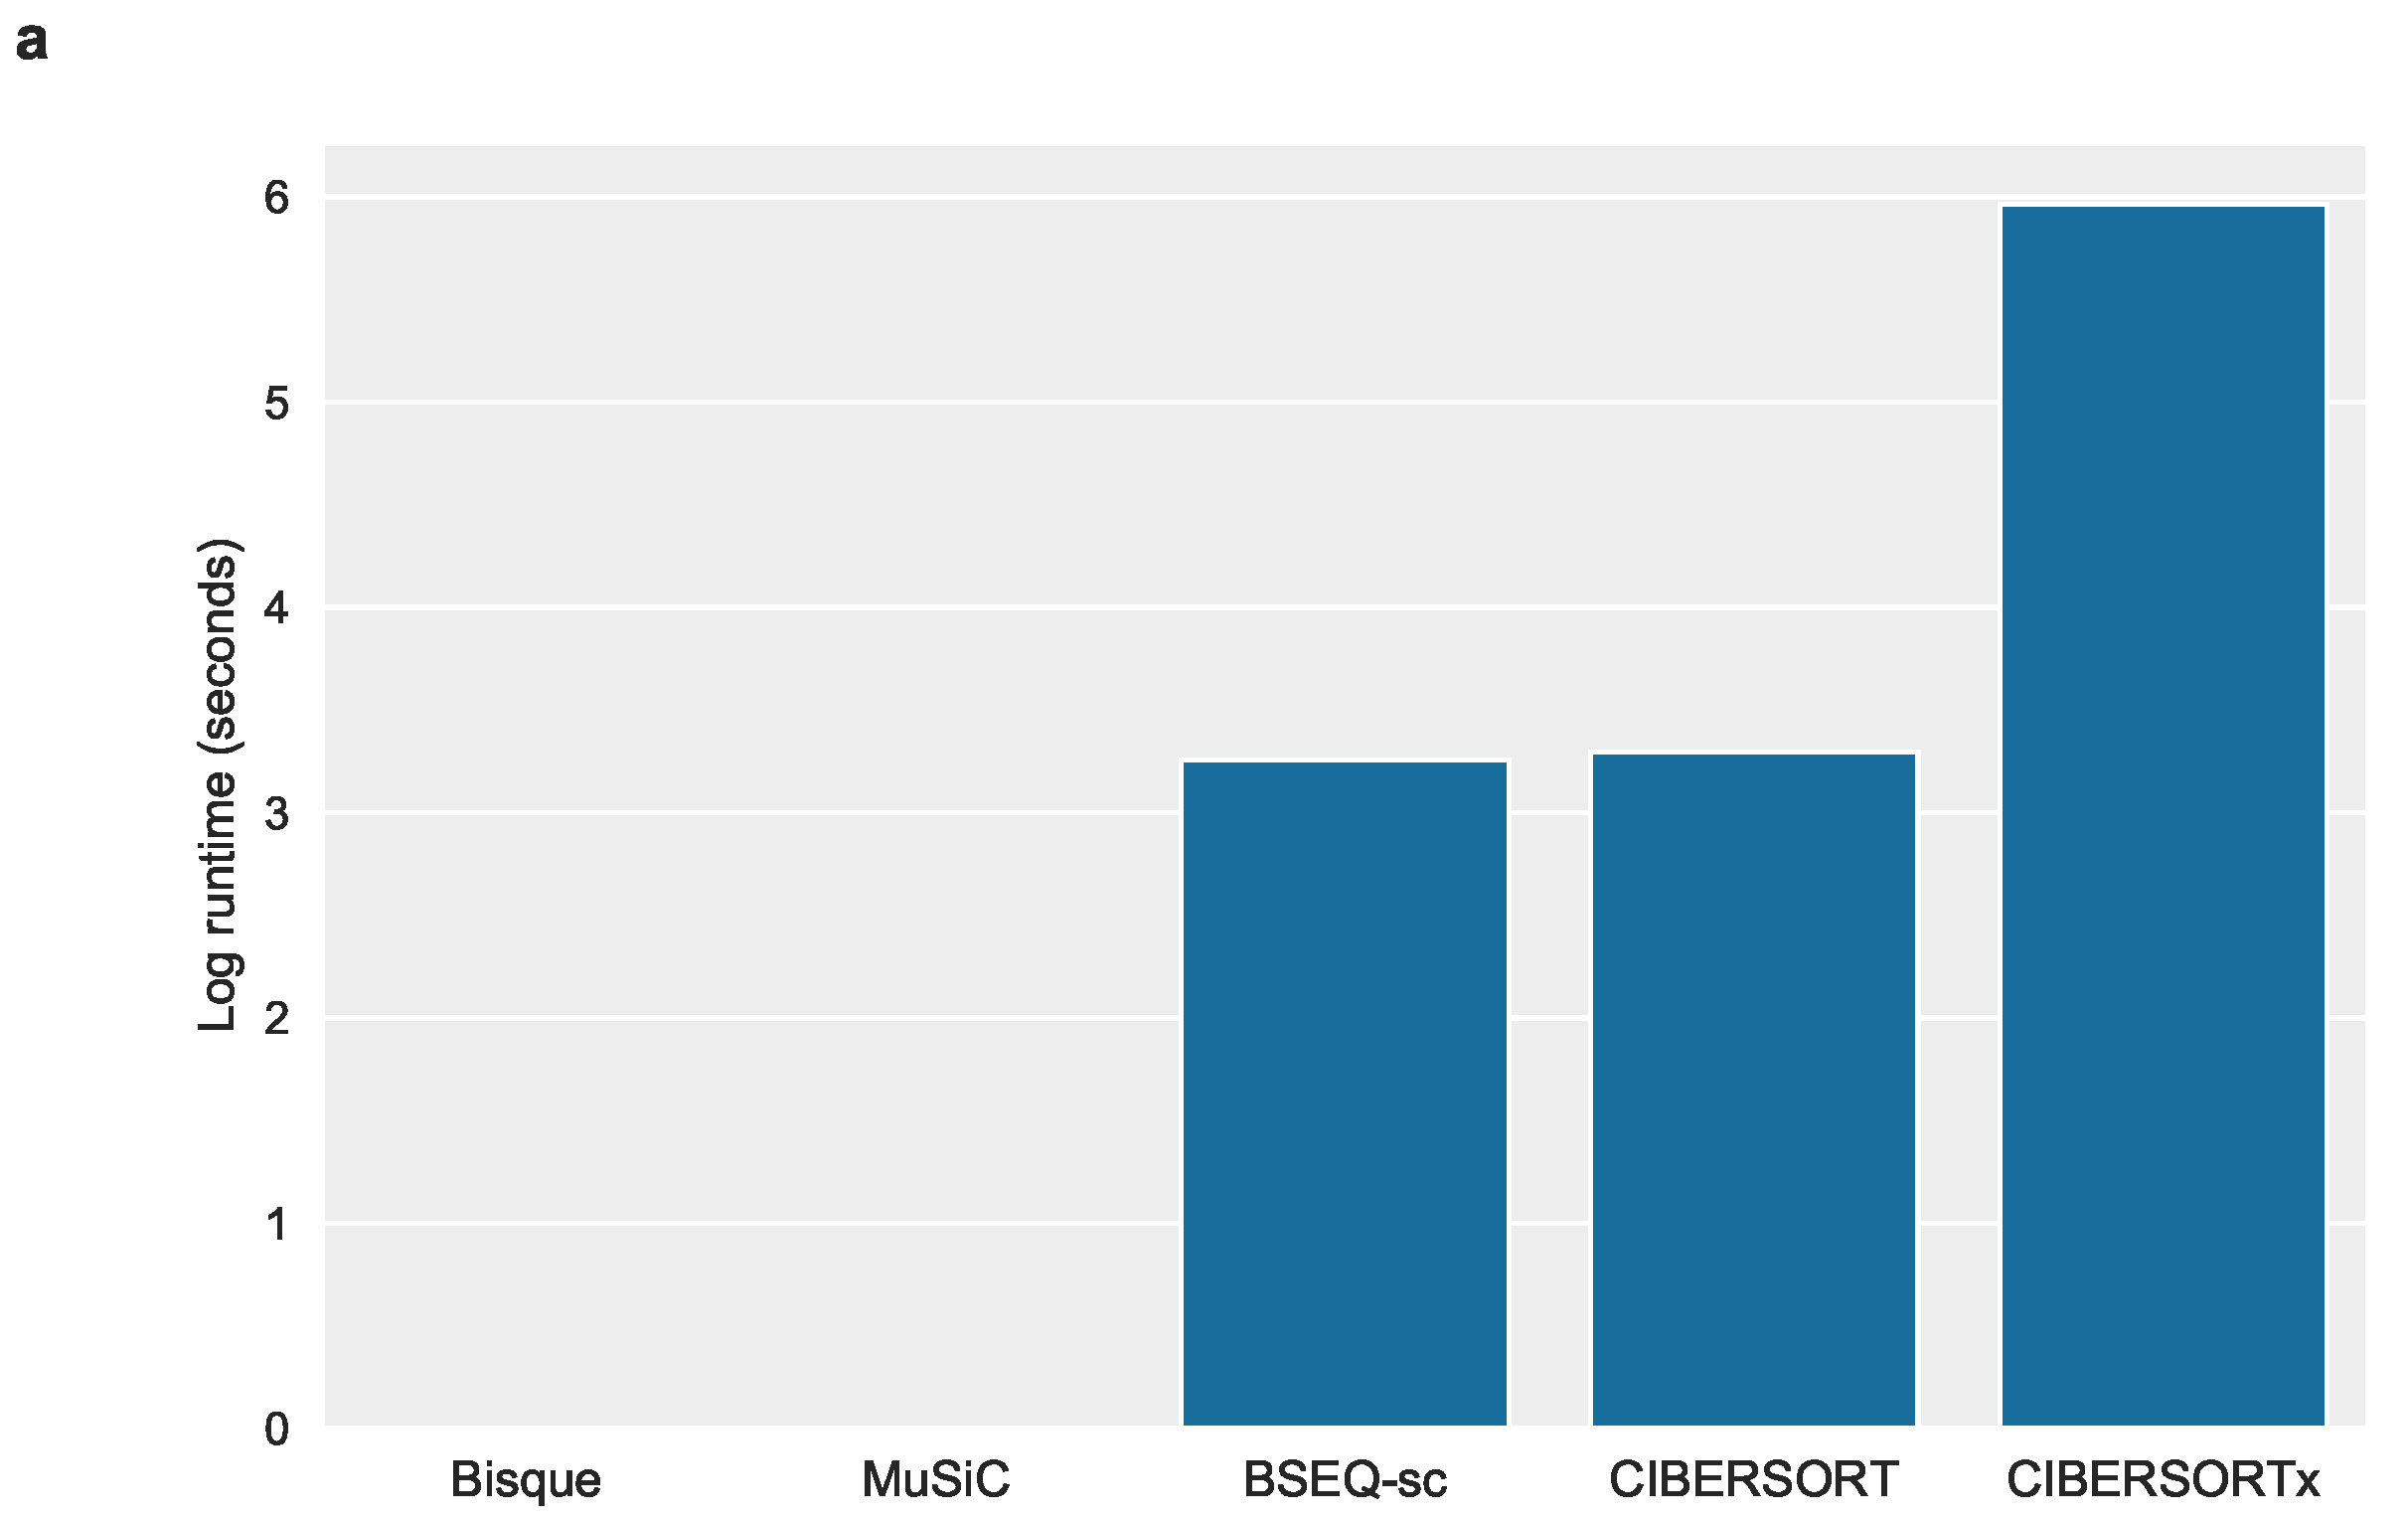
\includegraphics[scale=.19]{chapter2/figures/fig5a.pdf}
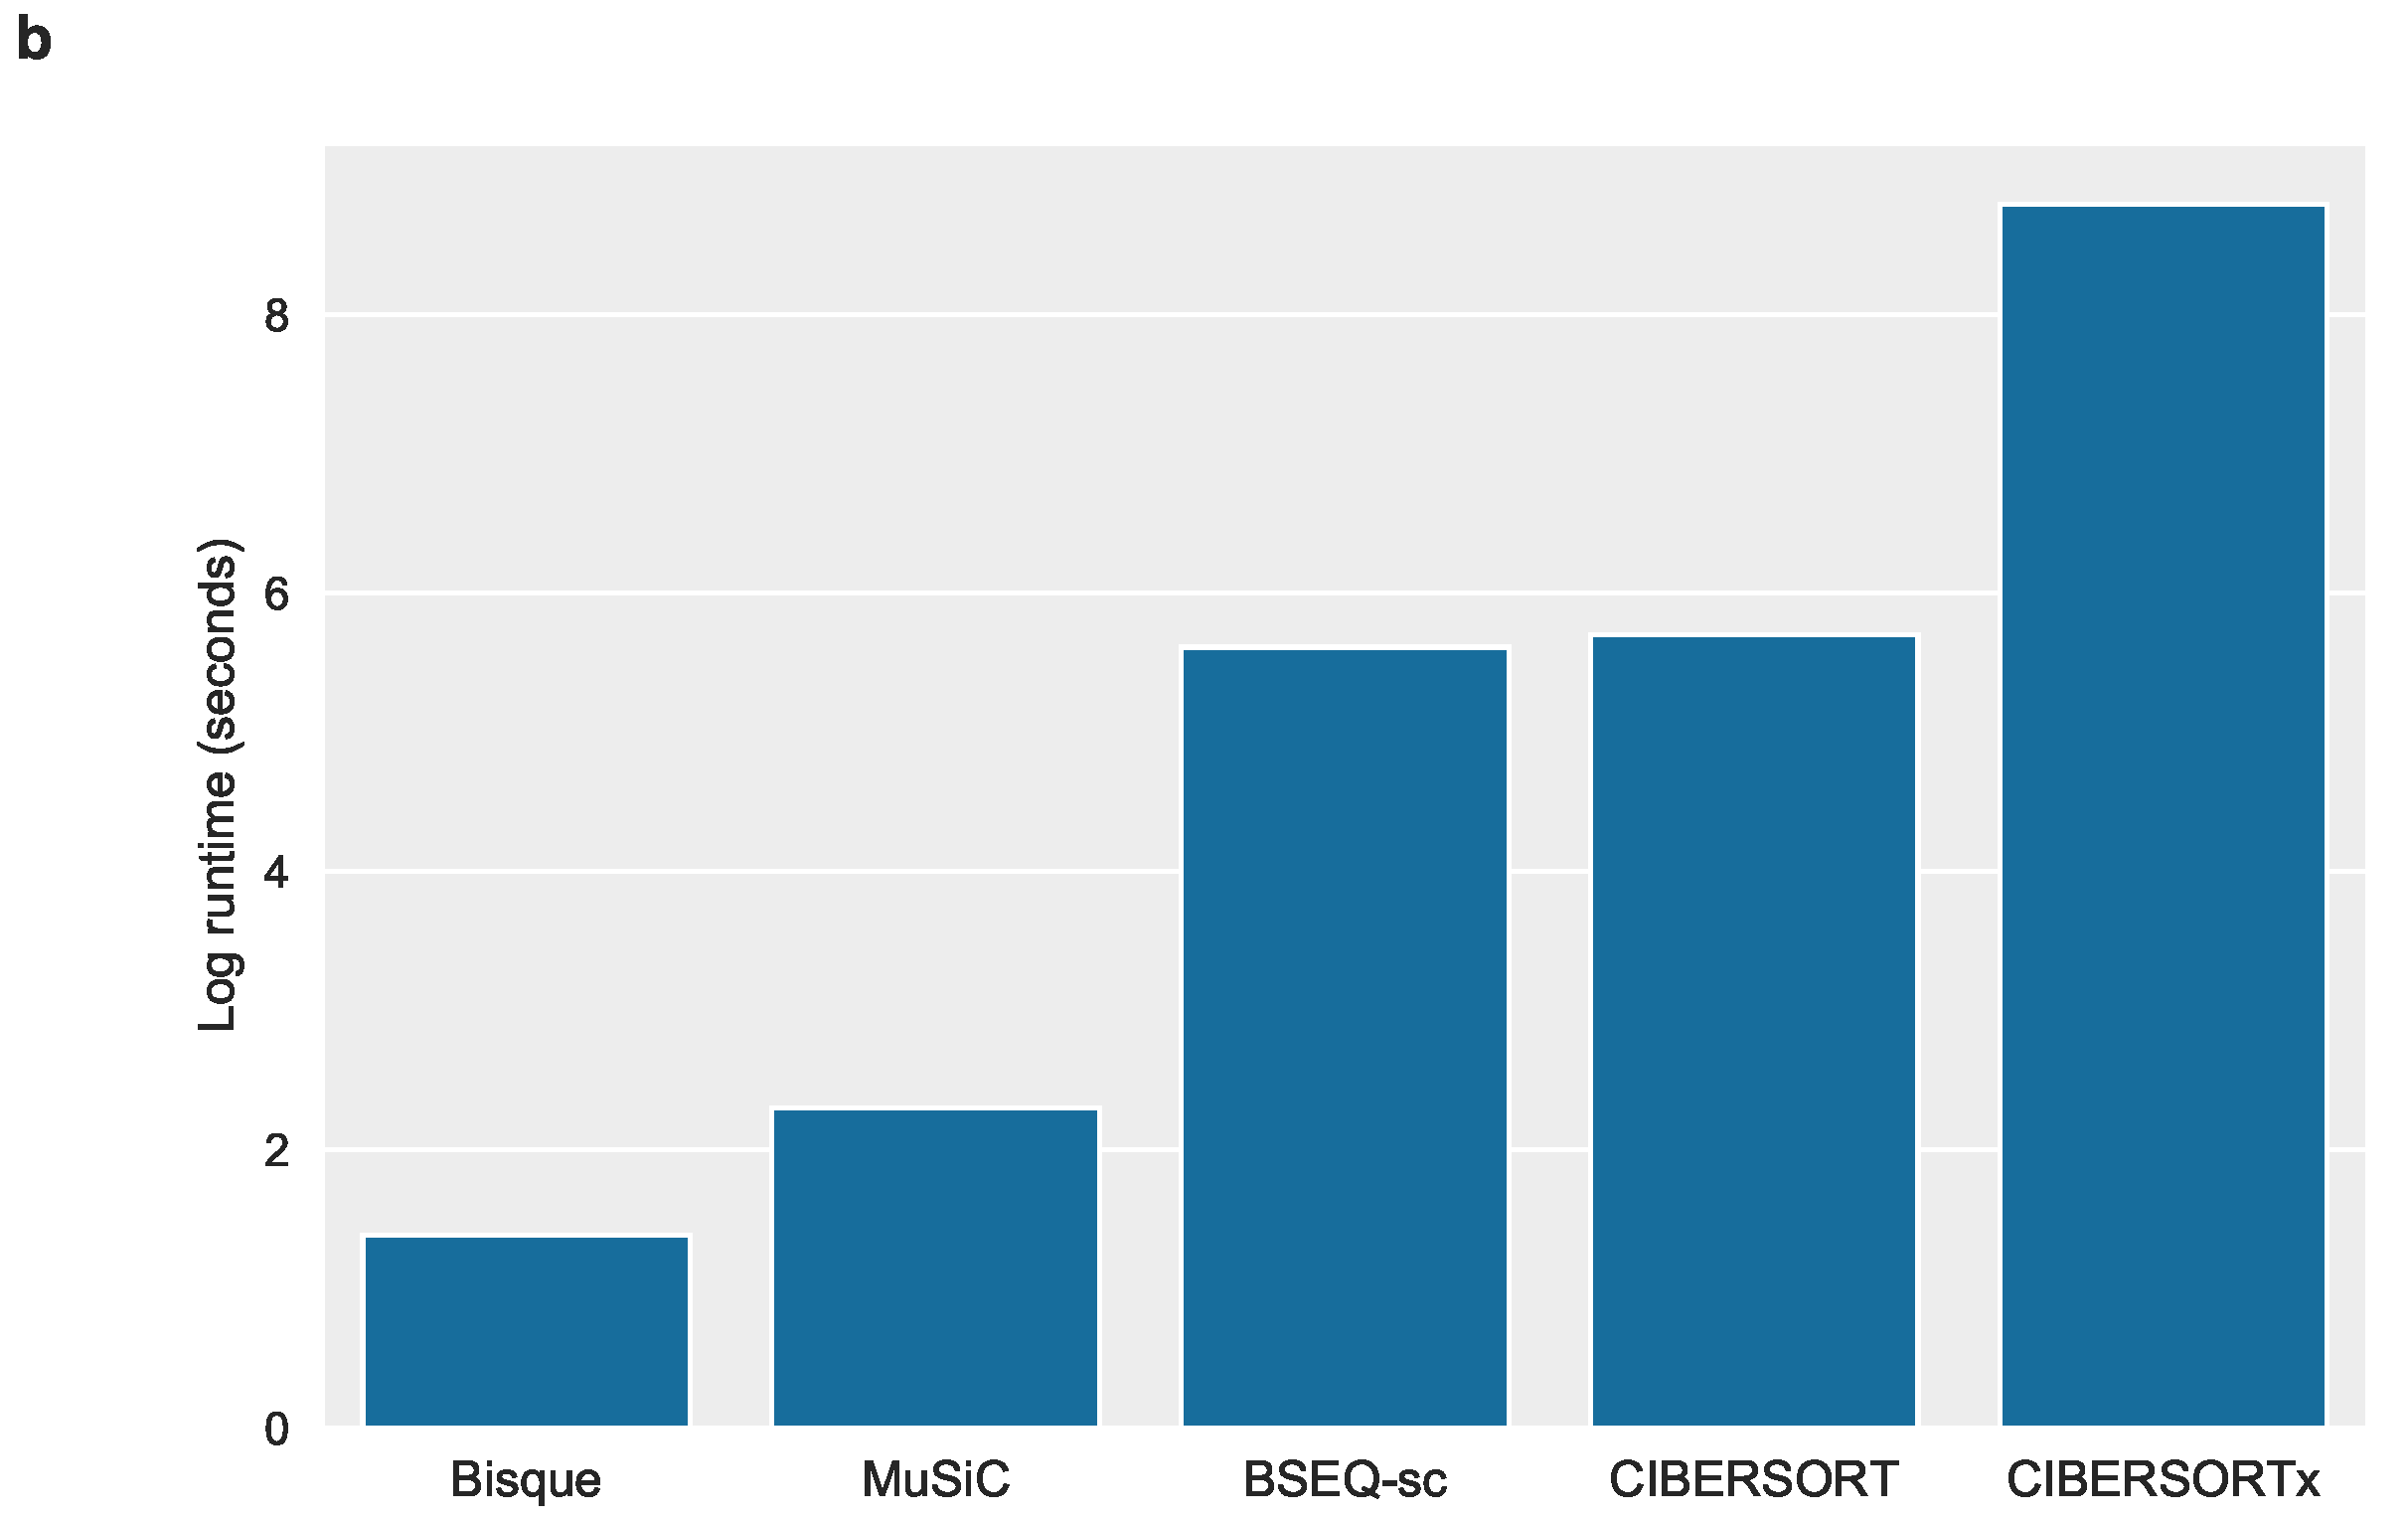
\includegraphics[scale=.19]{chapter2/figures/fig5b.pdf}
\caption{
    Runtime comparisons in log-transformed seconds for benchmarked reference-based decomposition methods.
    (\textbf{a}) Runtime for subcutaneous adipose dataset, which included 100 RNA-seq samples and 6 snRNA-seq samples with around 1,800 nuclei per individual.
    (\textbf{b}) Runtime for dorsolateral prefrontal cortex dataset, which included 628 RNA-seq samples and 8 snRNA-seq samples. We benchmarked each method using around 2,125 nuclei per snRNA-seq sample.
    }
\label{fig:fig2.5}
\end{figure}


\subsection{Robustness of the reference-based decomposition model}

Our reference-based decomposition method is based on the assumption that cell populations are equally represented in single-cell and bulk RNA sequencing of the same tissue samples. Since this assumption may be violated~\cite{Schelker2017-ms}, we explored the performance of our model as we relaxed this assumption in simulations. First, we simulated snRNA-seq data where cell proportions were increasingly biased. Using the DLPFC snRNA-seq data, we downsampled or upsampled the cells identified as microglia at varying levels and performed decomposition. Indeed, the absolute estimates produced by Bisque propagated these shifts in snRNA-seq proportions. However, we found that our estimates maintained their expected positive association with Braak stage, evidence for the correlation between these estimates and the true microglia proportions (Figure \ref{fig:supfig5}a).  Given these results, we suggest that users take note of this behavior if both the mean abundances are important for downstream analysis and the single-cell reference data is known to be significantly biased against specific cell populations of interest.
 
Next, we simulated a situation where an unknown cell population contributes to bulk expression but is not represented in the snRNA-seq reference data. For situations where this unknown contribution varies across the bulk dataset, we simulated bulk expression by mixing the observed bulk expression for the DLPFC dataset with increasing amounts of expression observed in the adipose dataset. To determine the effect of unknown cell populations on our model, we analyzed the distribution of residual norms produced by the method. These residual norms provide a measure of the difference between the vector of observed bulk and expression reference weighted by the estimated proportions across all genes for each individual. As we increased the contribution from unknown cell types, the residual norm values tend to increase (Figure \ref{fig:supfig5}b). In our simulation framework, this variability in unknown cell type contribution could be qualitatively identified by the presence of a multimodal residual norm distribution. 

Given that single-cell datasets still remain relatively small compared to bulk datasets, we also explored the impact of sample size in the reference single-cell data on the performance of Bisque. In the DLPFC dataset, we saw a drop in performance when using less than four randomly selected snRNA-seq samples (Figure \ref{fig:supfig5}c). This threshold is likely to differ between experiments, though we recommend at least three single-cell samples to generate reference data. 

Finally, since marker gene selection can vary between studies, we were interested in the performance of Bisque as we varied the number of marker genes. Again, we measured cell type proportion estimation performance for microglia in the DLPFC dataset by correlating the estimates with Braak stage, which is known to have a positive association. We recalculated this correlation as we removed marker genes for this cell type. We removed marker genes in order of both decreasing and increasing log-fold-change, which provides a measure of the importance of marker genes for identifying this cell type. In both procedures, we observe that as we remove an increasing percentage of the 102 identified marker genes, performance remains stable until a shared drop off point around 75\% (Figure \ref{fig:supfig5}d). Since we observed this trend in both marker gene removal schemes, we assume that a relatively few number of marker genes, regardless of their log-fold-change magnitude, can be used to accurately estimate cell type proportions. These results suggest that as long as a core set of marker genes are present, variations in less important marker genes will have little effect on downstream analyses.

\begin{figure}
\centering
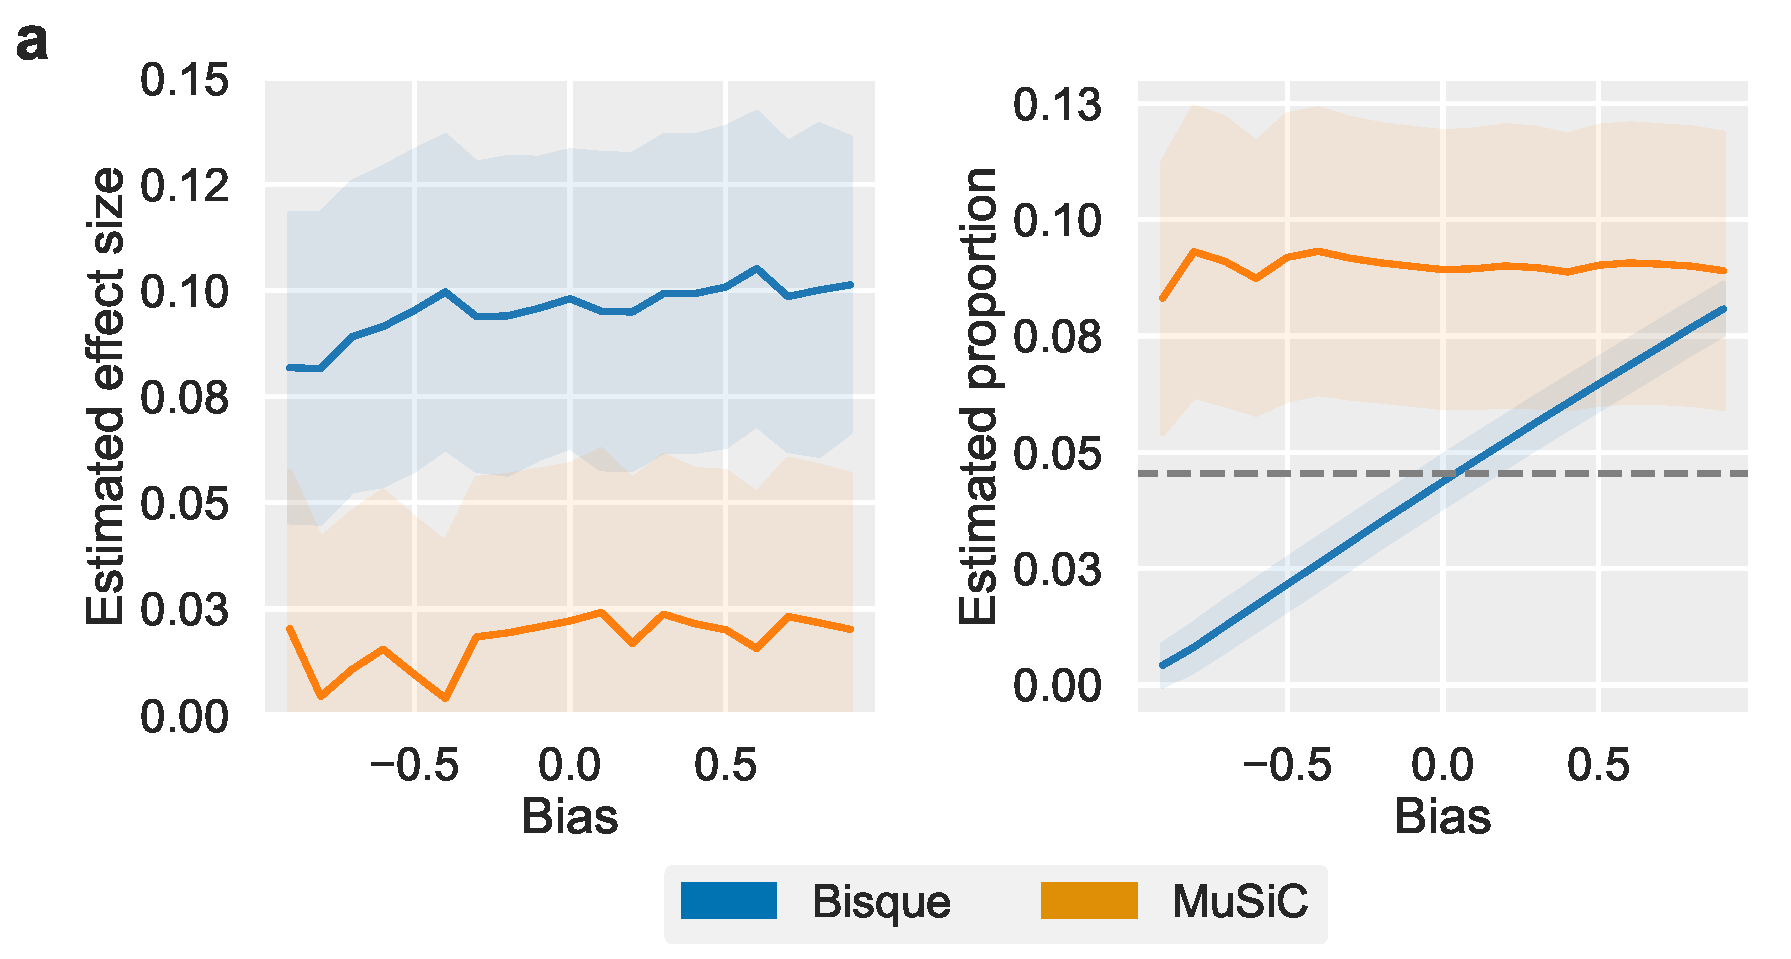
\includegraphics[scale=\figscale]{chapter2/figures/supp_fig_5ab.pdf} 
\hspace*{1cm}
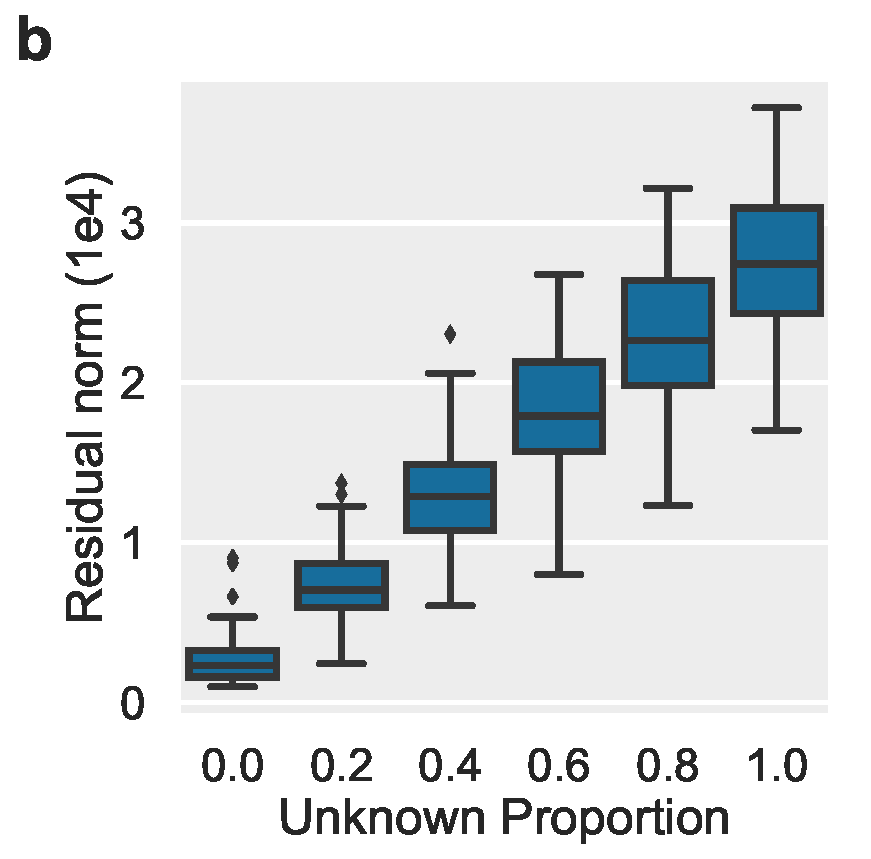
\includegraphics[scale=\figscale]{chapter2/figures/supp_fig_5c.pdf} 
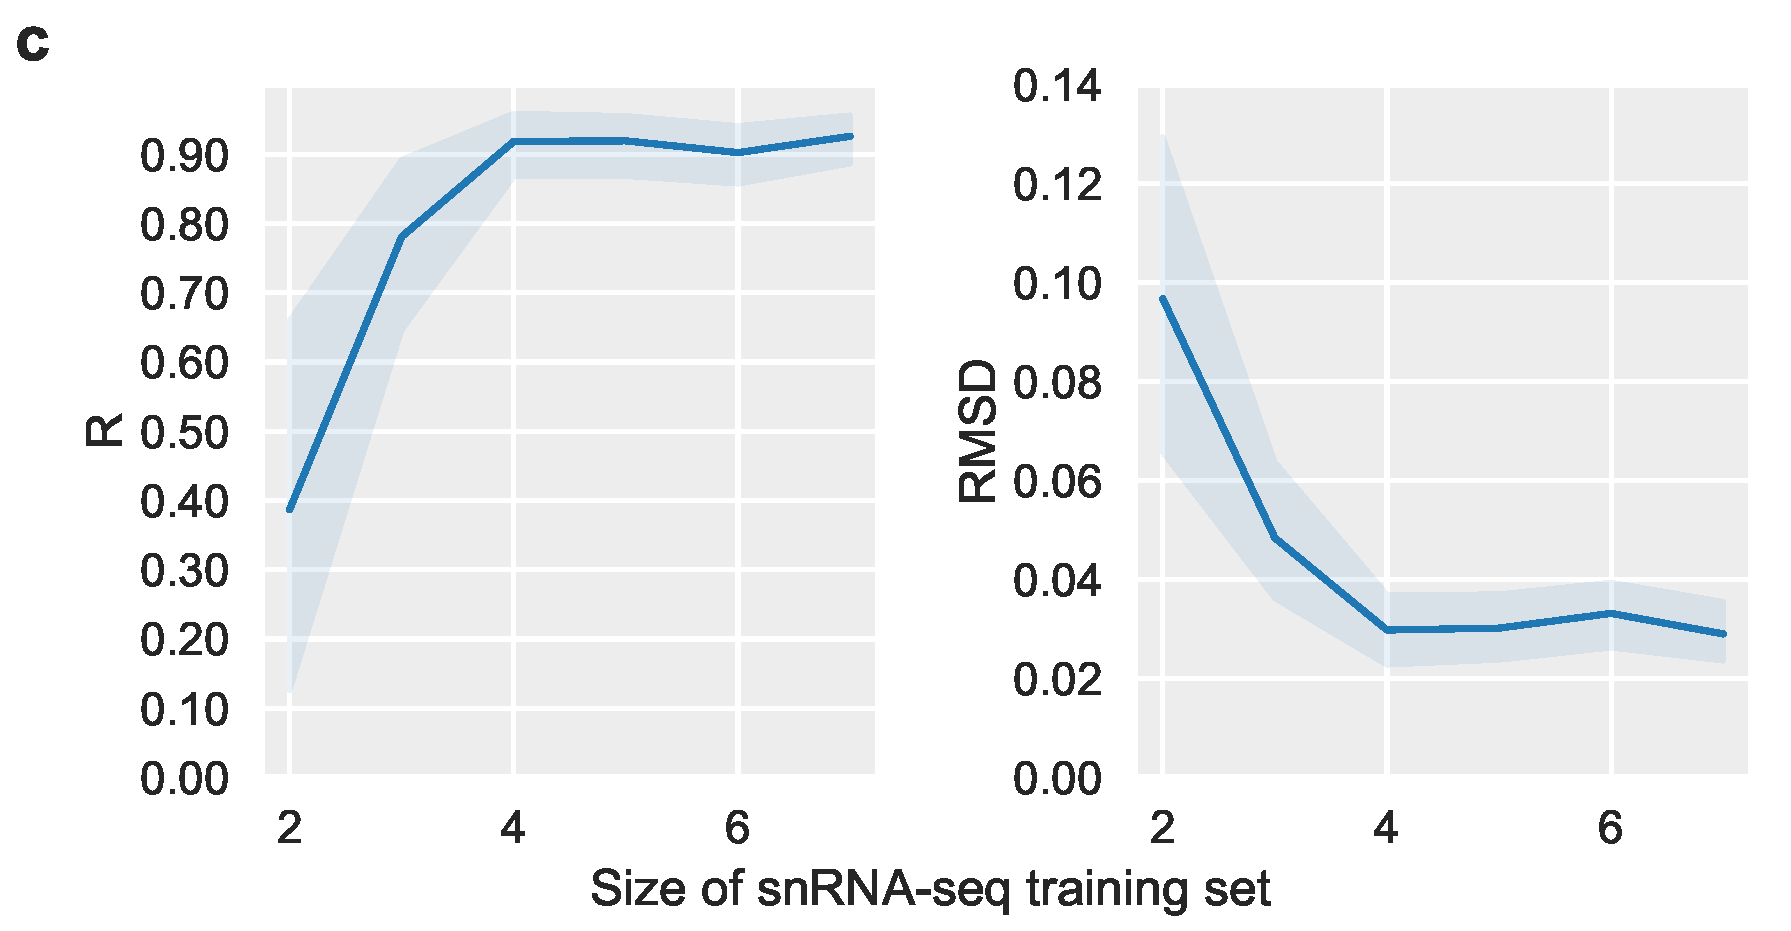
\includegraphics[scale=0.27]{chapter2/figures/supp_fig_5d.pdf}
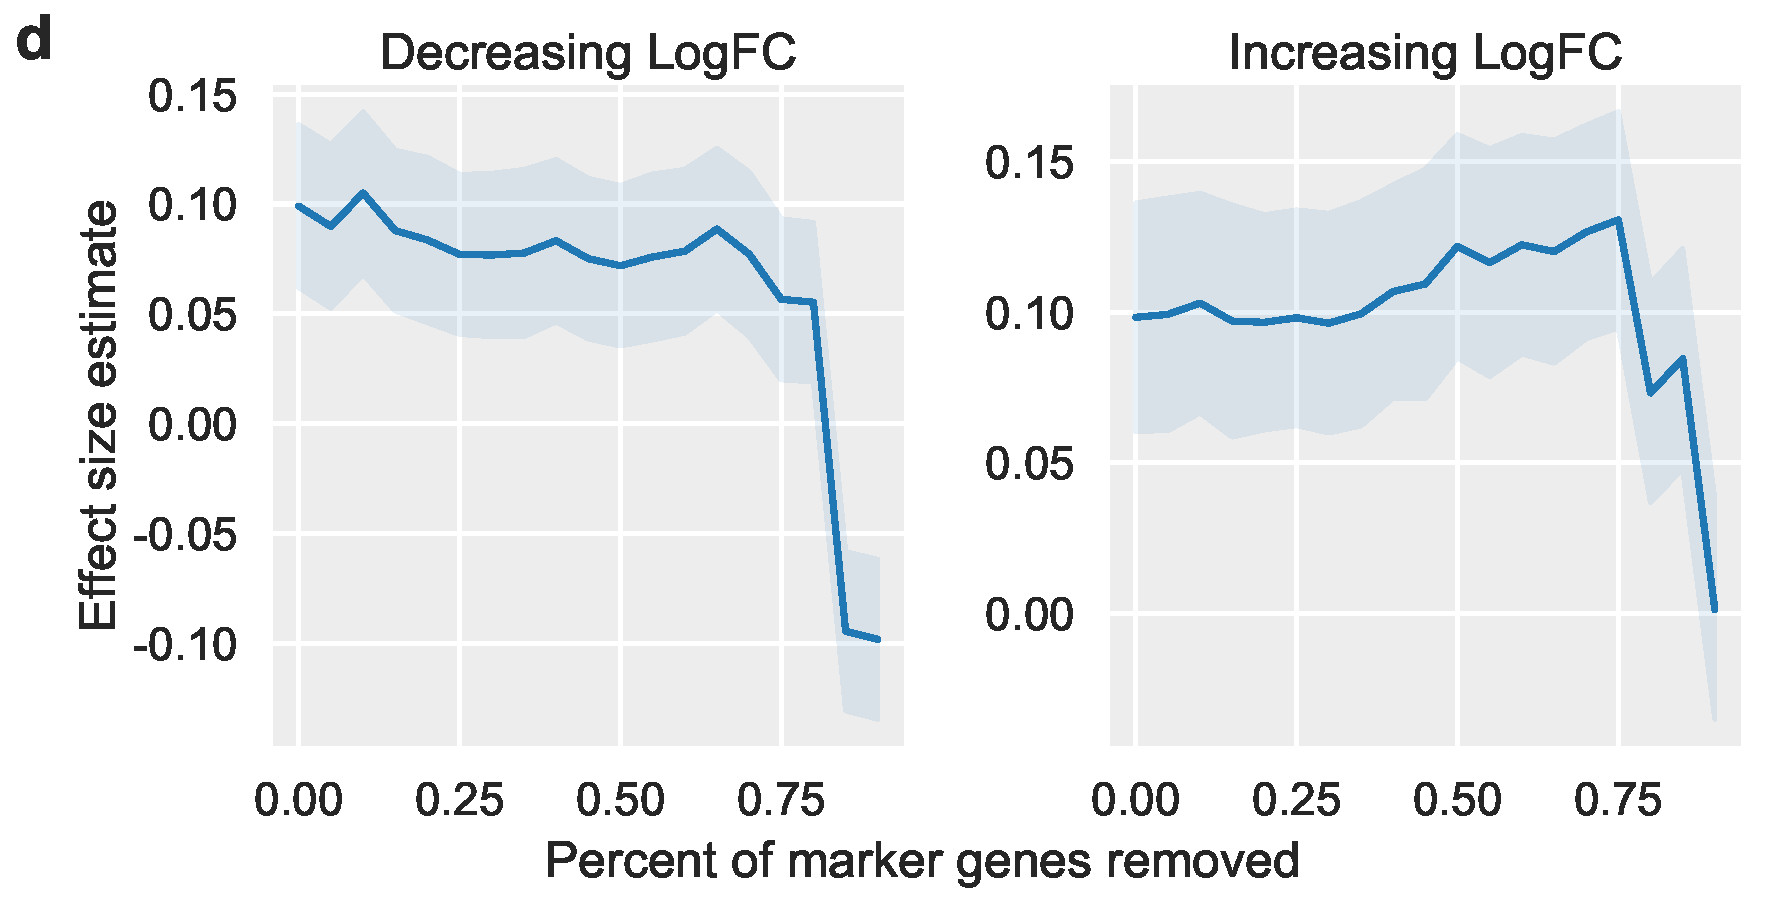
\includegraphics[scale=0.27]{chapter2/figures/supp_fig_5e.pdf}
\caption{
        Robustness of the reference-based decomposition model. 
        (\textbf{a}) Microglia cells in the DLPFC snRNA-seq data were upsampled or downsampled at various percentages, denoted as bias on the x-axis. Decomposition performance, measured as the estimated effect size of microglia proportion on Braak stage (which is expected to be positive) on the y-axis was consistent for each method as the bias in the snRNA-seq reference varied (left). The simulated bias propagates to the estimated proportions for Bisque(right). Shaded regions indicate standard error of estimates.  
        (\textbf{b}) In order to model the severity of the sample discordance due to unknown cell fractions, we compared the amount of adipose contamination, denoted as unknown proportion on the x-axis, to the residuals from the Bisque model (y-axis).
        (\textbf{c}) Leave-one-out cross-validation performance in the DLPFC dataset after utilizing random subsamples of the snRNA-seq data as a reference. Performance measured in terms of Pearson correlation (left) and RMSD (right). Shaded regions indicate 95\% confidence interval.
        (\textbf{d}) At each amount of marker genes removed (x-axis), performance was measured as the effect size of the estimated microglia proportion on Braak stage (y-axis). Genes were removed in order of decreasing (left) or increasing (right) log-fold-change. Shaded regions indicate standard error of estimates.
        }
\label{fig:supfig5}
\end{figure}

\subsection{Marker-based decomposition using known cell type marker genes }

While a reference profile from snRNA-seq can help to decompose bulk level gene expression, it may not be available for the same data set. The majority of bulk RNA-seq data sets do not have corresponding snRNA-seq data in the same set of individuals. However, marker gene information from prior experiments can still be applied to distinct expression data sets of the same tissue. The basis of most decomposition methods relies on the logic that as the proportion of a cell type varies across individuals, the expression of its marker genes will tend to correlate in the same direction as its cell type proportion. This linear co-variation can be captured in a principal components analysis (PCA). Under the same argument, the more cell type-specific a marker gene is, the more its expression will reflect its cell type proportion. These observations form the basis for BisqueMarker, a weighted PCA-based (wPCA) decomposition approach. Genes that are more specifically expressed within a cell type will provide more information than genes with shared expression across cell types. To estimate cell type proportions without the use of cell type-specific gene expression information, we applied wPCA to bulk-level adipose tissue expression.

For each cell type, we extracted the first PC from a wPCA of the expression matrix of its markers. The expression matrix was corrected for the first global expression PC as a covariate so that wPCA estimates would not reflect technical variation. We first confirmed that these genes were distinct across cell types. If 2 cell types share a high proportion of marker genes, the wPCA estimates from bulk RNA-seq will correlate highly. We then investigated whether the second or third PC could have represented cell type proportions. The percent of variance explained by the first PC was typically 30-60\% across adipose cell types, and additionally, over 90\% of the markers correlated in the same direction as the first PC. In contrast, roughly 50-70\% of markers correlated in the same direction as the second or third PC. As performed for reference-based decomposition, we correlated phenotypes with cell type proportions estimated by BisqueMarker. We identified the same associations as with reference-based decomposition, demonstrating its validity when a reference is not available (Tables \ref{table:suptable2.1a}, \ref{table:suptable2.1b}, \ref{table:suptable2.1c}). Similarly, we observed the same trends between estimated cell type abundances and phenotypes as we did using our reference-based method in the DLPFC cohort (Tables \ref{table:suptable2.2a}, \ref{table:suptable2.2b}). 

\section{Discussion}

Bisque effectively leverages single-cell information to decompose bulk expression samples, outperforming existing methods in datasets with snRNA-seq data available. In simulations, we demonstrated that the decomposition accuracy of Bisque is robust to increasing variation between the generation of the reference profile and bulk expression, which is a significant issue when comparing snRNA-seq and bulk RNA-seq data. In observed bulk expression, our reference-based method accurately estimates cell proportions that are consistent with previously reported distributions and reliably detects rare cell types. We found that these estimates consistently follow expected trends with measured phenotypes, suggesting that cell-specific estimates of proportion are sufficiently accurate to extract relevant biological signals. In addition, differences in tissue structure can lead to significant differences in the quality of single-cell expression data~\cite{Nguyen2018-gv}. We demonstrated the improved performance of our method in adipose and DLPFC, two distinct tissues, suggesting that Bisque is robust across different tissue types.

The cell type proportion estimates determined by Bisque may be utilized to effectively identify cell-type-specific interactions, such as expression quantitative trait loci (eQTLs), and adjust for confounding effects from variability in cell populations. With this reference-based approach, single-cell sequencing of a subset of samples from large-scale bulk expression cohorts can provide high power to detect cell-specific associations in complex phenotypes and diseases. 

However, we note that there are limitations to this reference-based method that users should consider. First, if the number of individuals with single-cell data available is small, the reference profile and gene-specific transformations may become unreliable. In addition, a key assumption of our transformation framework is that single-cell based estimates of cell proportions accurately reflect the true proportions we wish to estimate. As a result of this assumption, Bisque provides estimates of cell proportions reported by the single-cell technology used to generate the reference data. Given that snRNA-seq can provide less bias in isolating specific cell types compared to scRNA-seq~\cite{Wu2019-pq,Bakken2018-nt}, we expect these estimates to be useful for downstream analyses such as those previously discussed. Nevertheless, the accuracy of Bisque may decrease if the proportion of cell types captured by single-cell experiments differs significantly from the true physiological distributions. Therefore, we advise users to take caution if there is a known significant bias in the single-cell measurements of a tissue, such as severe underrepresentation of a cell type of interest, that can affect downstream analysis. Our results demonstrate that even with these limitations, Bisque can be used to provide cell-type specific biological insight in relevant datasets.

In cases where these described issues may be significant, BisqueMarker provides cell type abundance estimations using only known marker genes. While this reference-free method may be less accurate than reference-based methods, it does not depend on single-cell based estimates of cell proportions or expression profiles, but rather on the fact that the expression in certain genes differs across different cell types; moreover, this method also does not model explicitly the expression level, and it is thus robust to biases in the single cell sequencing protocol. We found that BisqueMarker estimates followed expected trends with measured phenotypes; however, it should be noted that this method estimates relative differences in abundances that cannot be compared across cell types. Also, given the semi-supervised nature of this method, these cell type abundance estimates may include signals from technical or other biological variation in the data. Therefore, we highly suggest applying this method to data that is properly normalized with sources of undesired variation removed. Bisque is available as an R package on CRAN (BisqueRNA) and at \url{https://github.com/cozygene/bisque}.
                         % Chapter 2
%\chapter{An efficient linear mixed model framework for meta-analytic association studies across multiple contexts}

\section{Background}

    Over the last decade, the scale of genomic datasets has steadily increased. These datasets have grown to the size of hundreds of thousands of individuals \cite{Bycroft2018} with millions soon to come \cite{allofus}. Similarly, datasets for transcriptomics and epigenomics are growing to thousands of samples \cite{gtex, GTEx_Consortium2020-xx, ewas}. These studies provide valuable insight into the relationship between our genome and complex phenotypes \cite{gwas}. 
    
    Identifying these associations requires statistical models that can account for biases in study design that can negatively influence results through false positives or decreased power. Linear mixed models (LMMs) have been a popular choice for controlling these biases in genomic studies, utilizing variance components to account for issues such as population stratification \cite{Kang}. These models can also be used to analyze studies with repeated measurements from individuals, such as replicates or measurements across different contexts. Meta-Tissue  \cite{Sul} is a method that applies this model in the context of identifying expression quantitative trait loci (eQTLs) across multiple tissues. In this framework, gene expression is measured in several tissues from the same individuals and the LMM is utilized to test the association between these values and genotypes. A meta-analytic approach is used to combined effects across multiple tissues to increase the power of detecting eQTLs. This approach has also been applied to increase power in genome-wide association studies (GWAS) by testing the association between genotypes and multiple related phenotypes \cite{Joo}. 
    
    However, these approaches are computationally intensive. Existing approaches for fitting these models are cubic in time complexity with respect to the number of samples across all contexts \cite{Kang, Zhou}. Here, we present an ultra-fast LMM framework specifically for multiple-context studies. Our method, mcLMM, is linear in complexity with respect to the number of individuals and allows for statistical tests in a manner of hours rather than days or years with existing approaches. To illustrate the computational efficiency of mcLMM, we compare the runtime and memory usage of our method with EMMA and GEMMA \cite{Kang, Zhou}, two popular approaches for fitting these models. We further apply mcLMM to identify a large number of eQTLs in the Genotype-Tissue Expression (GTEx) dataset \cite{GTEx_Consortium2020-xx} and compare our results from METASOFT \cite{Metasoft}, which performs the meta-analysis of the mcLMM output, to a recent meta-analytic approach known as mash \cite{Urbut2019}. Finally, to demonstrate the practicality of mcLMM on modern datasets, we perform a multiple-phenotype GWAS combining over a million observations sampled from hundreds of thousands of individuals in the UK Biobank \cite{Bycroft2018} within hours.

\section{Methods}

   \subsection{Linear Mixed Model}
        For multi-context experiments with $n$ individuals, $t$ contexts, and $c$ covariates, we fit the following linear mixed model
        
        \begin{equation}
            \mathbf{y} = X\beta + \mathbf{u} + \mathbf{e}
        \end{equation}
        
        \noindent where $\mathbf{u} \sim N(0,\sigma_g^2 K)$, $\mathbf{e} \sim N(0,\sigma_e^2 I)$,  $\mathbf{y} \in R^{nt}$ is a vectorized representation of the responses, $X \in R^{nt \times tc}$ is the matrix of covariates,
        $\beta \in R^{tc}$ is the vector of estimated coefficients, $K \in R^{nt \times nt}$ is a binary matrix where $K_{i,j} = 1$ 
        indicates that sample $i$ and sample $j$ in $Y$ come from the same individual, and $I \in R^{nt \times nt}$ is an identity matrix.
        $X$ is structured such that both an intercept and the covariate effects are fit within each context. For sake of simplicity, dimensions
        of $nt$ assume that there is no missing data; however, this is not a requirement for the model.
        
        The full and restricted log-likelihood functions for this model are
        \begin{equation}
            l_F(\mathbf{y}; \beta, \sigma_g, \delta) = \frac{1}{2}\left[-N\log{(2\pi\sigma^2_g)} - \log(|H|) - \frac{1}{\sigma^2_g}(\mathbf{y}-X\beta)^T H^{-1} (\mathbf{y}-X\beta)\right]
        \end{equation}
        \begin{equation}
            l_R(\mathbf{y}; \beta, \sigma_g, \delta) = l_F(\mathbf{y}; \beta, \sigma_g, \sigma_e) + \frac{1}{2}\left[tc\log(2\pi\sigma^2_g) + \log{(|X^TX|)} - \log{(|X^TH^{-1}X|)}\right]
        \end{equation}
        where $N$ is the total number of measurements made across the individuals and contexts, $\delta = \frac{\sigma^2_e}{\sigma^2_g}$, and $H = K + \delta I$  \cite{Welham}. These likelihood functions are maximized with the generalized least squares estimator $\hat{\beta} = (X^TH^{-1}X)^{-1}X^TH^{-1}\mathbf{y}$ and $\hat{\sigma^2_g} = \frac{R}{N}$ in the full log-likelihood and $\hat{\sigma^2_g} = \frac{R}{N-tc}$ in the restricted log-likelihood, where $R = (\mathbf{y}-X\hat{\beta})^TH^{-1}(\mathbf{y}-X\hat{\beta})$.  Our goal is to maximize these likelihood functions to estimate the optimal $\hat{\delta}$.
    
    \subsection{Likelihood refactoring in the general case}
        The EMMA algorithm optimizes these likelihoods for $\delta$ by refactoring them in terms of constants calculated from eigendecompositions of $H$ and $SHS$, where $S = I - X(X^TX)^{-1}X^T$, that allow linear complexity optimization iterations with respect to the number of individuals  \cite{Kang}. The GEMMA algorithm further increases efficiency by replacing the $SHS$ eigendecomposition with a matrix-vector multiplication \cite{Zhou}. Both approaches require the eigendecomposition of at least 1 $N$ by $N$ matrix which is typically cubic in complexity. Here, we show that our specific definition of $K$ as a binary indicator matrix allows us to refactor these likelihood functions without any eigendecomposition steps. It should be noted that EMMA and GEMMA can fit this model for any positive semidefinite K, while mcLMM is restricted to the definition described above. 
        
        First, note that $H = K + \delta I$ is a block diagonal matrix (as exemplified in Equation 5). Specifically, each block corresponds to an individual $i$ with $t_i$ contexts measured and is equal to $[\mathbf{1}_{t_i} + \delta I_{t_i}] \in R^{t_i \times t_i}$, where $\mathbf{1}_{t_i}$ is a $t_i$ by $t_i$ matrix composed entirely of 1. These properties of $H$ make its eigendecomposition and inverse directly known.
        
        The eigenvalues of a block diagonal matrix are equal to the union of the eigenvalues of each block. Moreover, the eigenvalues of $[\mathbf{1}_{t_i} + \delta I_{t_i}]$ are $t_i + \delta$ with multiplicity 1 and $\delta$ with multiplicity $t_i - 1$. Therefore, $H$ has eigenvalues $\delta$ with multiplicity $N-n$ and $t_i + \delta$ for each $t_i$. This provides our first refactoring
        
        \begin{equation}
            \log{(|H|)} = (N-n)\log{(\delta)} + \sum_{i=1}^n \log{(t_i + \delta)}
        \end{equation}
        
        The inverse of a block diagonal matrix can also be computed by inverting each block individually. Moreover, using the Sherman-Morrison formula \cite{ShermanMorrison}, the inverse of $[\mathbf{1}_{t_i} + \delta I_{t_i}]$ is known
        
        \begin{equation}
            (\mathbf{1}_{t_i} + \delta I_{t_i})^{-1} =  -\frac{1}{t+\delta}\mathbf{1}_{t_i} + \frac{1}{\delta} I_{t_i}
        \end{equation}
        
        \noindent Given each entry of $H^{-1}$, we can show algebraically that
        
        \begin{equation}
            X^T H^{-1} X = \frac{1}{\delta}(E - D)
        \end{equation}
        \begin{equation}
            E_{i,j} = 
            \begin{cases} 
                \sum\limits_{\text{ind} \in f(i)} x_{\text{ind},g(i)}x_{\text{ind},g(j)}&\mbox{if } f(i) = f(j) \\
                0 & \mbox{if } f(i) \neq f(j)
            \end{cases}
        \end{equation}
        \begin{equation}
            D_{i,j} = \sum\limits_{g \in \text{groups}} \frac{1}{t_g + \delta} \sum\limits_{\text{ind} \in f(i),f(j),g}x_{\text{ind},g(i)}x_{\text{ind},g(j)}
        \end{equation}
        
        \noindent where $f(i) = i \% t$ (modulo operator) provides the context of a given 0-indexed column of X, $g(i) = i // t$ (integer division) provides the covariate of a given index. A group $g$ defines the set of individuals that share the same number of measured contexts $t_g$. The expression ``$\text{ind} \in f(i),f(j),g$" indicates the set of all individuals that have $t_g$ measured contexts that include context $i$ and $j$. 
        
        Note that with all values independent of $\delta$ pre-computed, specifically the sum of covariate interactions within the sets of individuals indicated above, $E$ is constant with respect to $\delta$ and each entry of the symmetric matrix $D$ can be calculated in linear time with respect to the number of groups, which is less than or equal to the number of contexts $t$. For a given $\delta$, we can compute $X^TH^{-1}X$ in $O(t(tc)^2)$ time complexity. Both the restricted and full log-likelihoods require the calculation of $(X^TH^{-1}X)^{-1}$. The restricted log-likelihood requires the additional calculation of $\log{(|X^TH^{-1}X|)}$. To calculate both of these terms, we perform a Cholesky decomposition of $X^TH^{-1}X = LL^*$, where $^*$ indicates the conjugate transpose. Given this decomposition, we can compute 
        
        \begin{equation}
            \log{(|X^TH^{-1}X|)} = \sum_{i=1}^{tc} L_{i,i}^2
        \end{equation}
        \begin{equation}
            (X^TH^{-1}X)^{-1} = (L^*)^{-1}L^{-1}
        \end{equation}
        
        \noindent These operations can be done in $O((tc)^3)$ time complexity. 
        
        Let $P(X)$ denote a projection matrix and $M(X) = (I-P(X))$. Note that both $P(X)$ and $M(X)$ are idempotent. The term remaining term in the likelihood functions, $R$, can be reformulated as follows
        \begin{align}
        \begin{split}
            \mathbf{y}- X\hat{\beta} & = \mathbf{y} - X(X^TH^{-1}X)^{-1}X^TH^{-1}\mathbf{y} \\
                                     & = (I - X(X^TH^{-1}X)^{-1}X^TH^{-1})\mathbf{y} \\
                                     & = (I - P(X))\mathbf{y} \\
                                     & = M(X)\mathbf{y}
        \end{split}
        \end{align}
        
        \begin{align}
        \begin{split}
            M(X)^TH^{-1} & = (I - X(X^TH^{-1}X)^{-1}X^TH^{-1})^T H^{-1} \\
                         & = (I - H^{-1}X(X^TH^{-1}X)^{-1}X^T)H^{-1} \\
                         & = H^{-1} - H^{-1}X(X^TH^{-1}X)^{-1}X^TH^{-1} \\
                         & = H^{-1}(I - X(X^TH^{-1}X)^{-1}X^TH^{-1}) \\
                         & = H^{-1}M(X)
        \end{split}
        \end{align}
    
        \begin{align}
        \begin{split}
            R & = (\mathbf{y}-X\hat{\beta})^TH^{-1}(\mathbf{y}-X\hat{\beta})    \\
              & = \mathbf{y}^TM(X)^TH^{-1}M(X)\mathbf{y} \\
              & = \mathbf{y}^TH^{-1}M(X)M(X)\mathbf{y} \\
              & = \mathbf{y}^TH^{-1}M(X)\mathbf{y} \\
              & = (\mathbf{y}^TH^{-1}\mathbf{y}) - (\mathbf{y}^TH^{-1}X(X^TH^{-1}X)^{-1}X^TH^{-1}\mathbf{y}) \\
              & = a - \mathbf{b}^T(X^TH^{-1}X)^{-1}\mathbf{b} \\
              & = a - \mathbf{b}^T(L^*)^{-1}L^{-1}\mathbf{b}
        \end{split}
        \end{align}
        The scalar $a$ and vector $\mathbf{b}$ are a function of $\delta$ and can be algebraically formulated as
        \begin{equation}
            a = \frac{1}{\delta}\left(\left(\sum_{i=1}^{N}\mathbf{y}_i^2\right) - \left(\sum\limits_{g \in \text{groups}} \frac{1}{t_g + \delta}\sum\limits_{\text{ind} \in g}(\sum\mathbf{y}_{\text{ind}})^2\right)\right)
        \end{equation}
        
        \begin{equation}
            \mathbf{b}_i = \frac{1}{\delta}\left(\left(\sum\limits_{\text{ind} \in \text{context(i)}} x_{\text{ind},g(i)}\mathbf{y}_{\text{ind},f(i)}\right) - \left(\sum\limits_{g \in \text{groups}} \frac{1}{t_g + \delta}\sum\limits_{\text{ind} \in f(i),g} x_{\text{ind},g(i)}(\sum\mathbf{y}_{\text{ind}}) \right)\right)
        \end{equation}
        where $\sum\mathbf{y}_{\text{ind}}$ indicates the sum of responses across all contexts for an individual. With values independent of $\delta$ pre-calculated, $a$ and $\mathbf{b}$ can be calculated in linear time with respect to the number of groups. 
        
        We can reformulate the entire likelihood functions as follows
        
        \begin{align}
        \begin{split}
            l_F(\mathbf{y}; \beta, \sigma_g, \delta) & = \frac{1}{2}\left[-N\log{(2\pi\sigma^2_g)} - \log(|H|) - \frac{1}{\sigma^2_g}(\mathbf{y}-X\beta)^T H^{-1} (\mathbf{y}-X\beta)\right] \\ 
                                                     & = \frac{1}{2}\left[-N\log{(2\pi\frac{R}{N})} - \log(|H|) - N\right] \\
                                                     & = \frac{1}{2}\left[-N\log{(2\pi\frac{R}{N})} - \left((N-n)\log{(\delta)} + \sum_{i=1}^n \log{(t_i + \delta)}\right) - N\right] \\
                                                     %& = \frac{1}{2}\left[-N\log{(2\pi\frac{a - \mathbf{b}^T(L^*)^{-1}L^{-1}\mathbf{b}}{N})} - \left((N-n)\log{(\delta)} +  \sum_{i=1}^n \log{(t_i + \delta)}\right) - N\right] \\
                                                     & \approx -N\log{(a - \mathbf{b}^T(L^*)^{-1}L^{-1}\mathbf{b})} - \left((N-n)\log{(\delta)} + \sum_{i=1}^n \log{(t_i + \delta)}\right) \label{lf_iter} 
        \end{split}
        \end{align}
        
        \begin{align}
        \begin{split}
            l_R(\mathbf{y}; \beta, \sigma_g, \delta) & = l_F(\mathbf{y}; \beta, \sigma_g, \sigma_e) + \frac{1}{2}\left[tc\log(2\pi\sigma^2_g) + \log{(|X^TX|)} - \log{(|X^TH^{-1}X|)}\right] \\
                                                     & \approx (tc-N)\log{(a - \mathbf{b}^T(L^*)^{-1}L^{-1}\mathbf{b})} \\
                                                     & -\left((N-n)\log{(\delta)} + \sum_{i=1}^n \log{(t_i + \delta)}\right) - \sum_{i=1}^{tc} L_{i,i}^2 \label{lr_iter} 
        \end{split}
        \end{align}
        
        Note that Equations \ref{lf_iter} and \ref{lr_iter} remove terms that are independent of $\delta$ since they are not required for finding its optimal value, indicated by the $\approx$ symbol. These likelihoods are maximized using the optimize function in R. For the full likelihood
        
        \begin{equation}
            \hat{\sigma}_g^2 = \frac{R}{\hat{\delta}N}
        \end{equation}
        
        \noindent For the restricted likelihood
        
        \begin{equation}
            \hat{\sigma}_g^2 = \frac{R}{\hat{\delta}(N-tc)}
        \end{equation}
        
        \noindent For both likelihoods
        
        \begin{equation}
            \hat{\sigma}_e^2 = \hat{\delta}\hat{\sigma}_g^2
        \end{equation}
    \subsection{Likelihood refactoring with no missing data}
    
        When there is no missing data, the likelihood functions can be further simplified. Note that in this case, $N = nt$ and all $t_i = t$. Hence,
        
        \begin{align}
        \begin{split}
            \log{(|H|)} & = (N-n)\log{(\delta)} + \sum_{i=1}^n \log{(t_i + \delta)} \\
                        & = (nt-n)log{(\delta)} + n\log{(t + \delta)}
        \end{split}
        \end{align}
        
        If the input terms $\mathbf{y}$, $X$, and $K$ are permuted resulting in samples being sorted in order of context, and the covariates in $X$ are sorted in order of context, we can decompose $H$ and $X$ into
        
        \begin{equation}
            H = (\mathbf{1}_{t} + \delta I_t) \otimes I_n 
        \end{equation}
        \begin{equation}
            X = I_t \otimes X_{\text{dense}}
        \end{equation}
        
        \noindent where $\otimes$ indicates the Kronecker product and $X_{\text{dense}} \in R^{n \times c}$ is a typical representation of the covariates for each individual without multiple contexts (i.e. samples as rows and covariates as columns). Utilizing the properties of Kronecker products, we can perform the following reformulation

        \begin{align}
        \begin{split}
            (X^TH^{-1}X)^{-1} & = ((I_t \otimes X^T_{\text{dense}})((\mathbf{1}_{t} + \delta I_t) \otimes I_n )^{-1}(I_t \otimes X_{\text{dense}}))^{-1} \\
                              & = ((\mathbf{1}_{t} + \delta I_t)^{-1} \otimes X^T_{\text{dense}}X_{\text{dense}})^{-1} \\
                              & = (\mathbf{1}_{t} + \delta I_t) \otimes (X^T_{\text{dense}}X_{\text{dense}})^{-1}
        \end{split}
        \end{align}
        
        \begin{align}
        \begin{split}
            \log{\left(|(X^TH^{-1}X)^{-1}|\right)} & = \log{(|(\mathbf{1}_{t} + \delta I_t) \otimes (X^T_{\text{dense}}X_{\text{dense}})^{-1}|)} \\
                                      & = \log{(|(\mathbf{1}_{t} + \delta I_t)|^c|(X^T_{\text{dense}}X_{\text{dense}})^{-1}|^t)} \\
                                      & = c\log{(|(\mathbf{1}_{t} + \delta I_t)|)} + t\log{(|(X^T_{\text{dense}}X_{\text{dense}})^{-1}|)} \\
                                      & = c\log{\left(\frac{1}{(t+\delta)\delta^{t-1}}\right)} + t\log{(|(X^T_{\text{dense}}X_{\text{dense}})^{-1}|)} \\
                                      & = c\left(-\log{(t+\delta)} - (t-1)\log{(\delta)}\right) + t\log{(|(X^T_{\text{dense}}X_{\text{dense}})^{-1}|)} \label{logXHX}
        \end{split}
        \end{align}
        
        \noindent Note that the remaining determinant in Equation \ref{logXHX} will not need to be calculated since it is independent of $\delta$. Next, we show that $\hat{\beta}$ is independent of $\delta$.
        
        \begin{align}
        \begin{split}
            \hat{\beta} & = (X^TH^{-1}X)^{-1}X^TH^{-1}\mathbf{y} \\
                        & = \left((\mathbf{1}_{t} + \delta I_t) \otimes (X^T_{\text{dense}}X_{\text{dense}})^{-1}\right)X^TH^{-1}\mathbf{y} \\
                        & = \left((\mathbf{1}_{t} + \delta I_t) \otimes (X^T_{\text{dense}}X_{\text{dense}})^{-1}\right)(I_t \otimes X^T_{\text{dense}})((\mathbf{1}_{t} + \delta I_t)^{-1} \otimes I_n )\mathbf{y} \\
                        & = \left((\mathbf{1}_{t} + \delta I_t) \otimes (X^T_{\text{dense}}X_{\text{dense}})^{-1}X^T_{\text{dense}}\right)((\mathbf{1}_{t} + \delta I_t)^{-1} \otimes I_n )\mathbf{y} \\
                        & = \left((\mathbf{1}_{t} + \delta I_t) (\mathbf{1}_{t} + \delta I_t)^{-1}\otimes (X^T_{\text{dense}}X_{\text{dense}})^{-1}X^T_{\text{dense}}\right)\mathbf{y} \\
                        & = \left(I_t\otimes (X^T_{\text{dense}}X_{\text{dense}})^{-1}X^T_{\text{dense}}\right)\mathbf{y}
        \end{split}
        \end{align}
        
        This form of $\hat{\beta}$ shows that the optimal coefficients are equivalent to fitting separate ordinary least squares (OLS) models for each context. We compute $\hat{\beta}$ by concatenating these OLS estimates. Given this term, we can also compute the residuals of this model $\mathbf{s} = (\mathbf{y} - X\hat{\beta})$ and reformulate $R$ as follows.
        
        \begin{align}
        \begin{split}
            R & = (\mathbf{y} - X\hat{\beta})^TH^{-1}(\mathbf{y} - X\hat{\beta}) \\
              & = \mathbf{s}^TH^{-1}\mathbf{s} \\
              & = \sum_{i=1}^{nt}\mathbf{s}_i \sum_{j=1}^{nt} \mathbf{s}_j H^{-1}_{j,i} \\
              & = \frac{1}{\delta} \left(\sum_{i=1}^{nt} \mathbf{s}_i^2 \right) + \frac{1}{\delta(t + \delta)} \left(-\sum_{i=1}^{n} \left(\sum \mathbf{s}_{\text{ind}(i)}\right)^2\right)
              %& = \frac{1}{\delta} \left(\sum_{i=1}^{nt} \mathbf{s}_i^2 \right) + \frac{1}{t + \delta} \left(-\sum_{i=1}^{nt} \mathbf{s}_i \sum \mathbf{s}_{\text{ind}(i)}\right)
        \end{split}
        \end{align}
    
        The term $ \sum \mathbf{s}_{\text{ind}(i)} $ denotes the sum of residuals for an individual across all contexts. Let $u = \sum_{i=1}^{nt} \mathbf{s}_i^2$ and $v = -\sum_{i=1}^{n} \left(\sum \mathbf{s}_{\text{ind}(i)}\right)^2$.
        \begin{equation}
            R = \frac{1}{\delta}u + \frac{1}{\delta(t + \delta)} v
        \end{equation}
        
        Now we can reformulate the log-likelihoods, omitting terms that do not depend on $\delta$.
        
        \begin{align}
        \begin{split}
            l_F(\delta) & = -nt\log{(R)} - \log(|H|) \\
                        & = -nt\log{\left(\frac{1}{\delta}u + \frac{1}{\delta(t + \delta)} v\right)} - (nt - n)\log{(\delta)} - n\log{(t+\delta)} \\
                        & = -nt\log{\left(u + \frac{1}{t+\delta} v\right)} + n \log{\left(\frac{\delta}{t+\delta}\right)}
        \end{split}
        \end{align}
        
        \begin{align}
        \begin{split}
            l_R(\delta) & = (tc-nt)\log{(R)} - \log(|H|) - \log{(|(X^TH^{-1}X)^{-1}|)} \\
                        %& = (tc-nt)\log{\left(\frac{1}{\delta}u + \frac{1}{\delta(t + \delta)} v\right)} - (nt - n)\log{(\delta)} - n\log{(t+\delta)} + c\log{(t + \delta)} + (tc-c)\log{(\delta)} \\
                        & = (tc-nt)\log{\left(u + \frac{1}{t+\delta} v\right)} + (c-n)\log{\left(\frac{t+\delta}{\delta}\right)}
        \end{split}
        \end{align}
        
        Both functions are differentiable with respect to $\delta$. Moreover, both derivatives have the same root
        
        \begin{equation}
            \hat{\delta} = \frac{-tu - v}{u+v}
        \end{equation}
    
        The scalar values $u$ and $v$ can be calculated by performing a separate OLS regression for each context, which can be completed in $O(t(nc^2 + c^3))$ time for a naive OLS implementation. Compared to the methods described above, this approach requires no iterative optimization and the estimate is optimal. Our implementation has a time complexity of $O(c^3 + nc^2 + tcn)$. 
        
    \subsection{Resource requirement simulation comparison}
        We installed EMMA v1.1.2 and manually built GEMMA from its GitHub source (genetics-statistics/GEMMA.git, commit 9c5dfbc). We edited the source code of GEMMA to prevent the automatic addition of intercept term in the design matrix (commented out lines 1946 to 1954 of src/param.cpp).
        
        Data were simulated using the mcLMM package. Sample sizes of 100, 200, 300, 400, and 500 were simulated with 50 contexts. Context sizes of 4, 8, 16, 32, and 64 were simulated with 500 samples. Data were simulated with $\sigma^2_e=0.2$ and $\sigma^2_g=0.4$ and a sampling rate of 0.5. Memory usage of each method was measured using the peakRAM R package (v 1.0.2). 
    
    \subsection{False positive rate simulation}
        We simulated gene expression levels in multiple tissues for individuals where there were no eQTLs. In other words, gene expression levels were not affected by any SNPs. We considered 10,000 genes and 100 SNPs resulting in one million gene-SNP pairs. We simulated 1,000 individuals. We also examined false positive rates with 500 and 800 individuals. We generated 49 such datasets where the number of tissues varied from 2 to 50. To simulate the genotypes for each subject, we randomly generated two haplotypes (vectors consisting of 0 and 1) assuming a minor allele frequency (MAF) of 30\%. To simulate gene expression levels from multiple tissues among the same individuals, we sampled gene expression from the following multivariate normal distribution:
        
        \begin{equation}
            \mathbf{y} \sim N(0,\sigma_g^2\mathbf{K} + \sigma_e^2\mathbf{I} )
        \end{equation}
        
        where $\mathbf{y}$ is an $N \times T$ vector representing the gene expression levels of $N$ individuals in $T$ tissues and $\mathbf{K}$ is an $NT \times NT$ matrix corresponding the correlation between the subjects across the tissues. $K_{i,j} = 1$ when $i$ and $j$ are from two tissues of the same individuals, $K_{i,j} = 0$ otherwise. Here, we let $\sigma_g = \sigma_e = 0.5$. We used a custom R function (included with the mcLMM package) to simulate data from this distribution, which is based on sampling from a smaller covariance matrix for each block of measurements from an individual.
        
        After generating the simulation datasets, we first ran mcLMM to obtain the estimated effect sizes and their standard errors, as well as the correlation matrices. The results from mcLMM were used as the input of METASOFT for meta-analysis to evaluate the significance. False positive rate was calculated as the proportion of gene-SNP pairs with p-values smaller than the significance level ($\alpha = 0.05$).
    
    \subsection{True positive simulations}
        We developed the true positive simulation framework based on a previous study describing mash \cite{Urbut2019}. We simulated effects for 20,000 gene-SNP pairs in 44 tissues, 400 of which have non-null effects (true positives) and 19,600 of which have null effects. Let $\beta_{jr}$ denote the effects of the gene-SNP pair $j$ in context/tissue $r$ and $\beta_j$ is a vector of effects across various tissues, including null effects and non-null effects. We simulated the gene expression levels for 1,000 individuals as:
            \begin{equation}
                \mathbf{y} = \beta_{jr}^T X + \mathbf{e}
            \end{equation}
        where $X$ denotes the genotypes of the individuals that were simulated as described in the false positive rate simulation. $\mathbf{e} \sim N(0,\sigma_g^2\mathbf{K} + \sigma_e^2\mathbf{I})$, which is similar to the simulation in the false positive rate simulation. For $\beta_j$, we defined two types of non-null effects and simulated them in different ways:
        \begin{itemize}
            \item Shared, structured effects: non-null effects are shared in all tissues and the sharing is structured. The non-null effects are similar in effect sizes and directions (up-regulation or down-regulation) across all tissues, and this similarity would be stronger among some subsets of tissues. For 19,600 null effects, we set $\beta_j=0$. For 400 non-null effects, we assumed that each $\beta_j$ independently followed a multivariate normal distribution with mean 0 and variance $\omega U_k$,
            where $k$ is an index number randomly sample from ${1,\ldots,8}$. $\omega = |\omega^\prime|, \omega^\prime \sim N(0, 1)$ represents a scaling factor to help capture the full range of effects. $U_k$ are $44 \times 44$ data-driven covariance matrices learned from the GTEx dataset, which are provided in \cite{Urbut2019}.
            \item Shared, unstructured effects: non-null effects are shared in all tissues but the sharing is unstructured or independent across different tissues. For 19,600 null effects, we set $\beta_j=0$. For 400 non-null effects, we sampled $\beta_j$ from a multivariate normal distribution with mean of 0 and variance of $0.01I$, where $I$ is a $44 \times 44$ identity matrix.
        \end{itemize}
        
        After simulating the gene expression levels $\mathbf{y}$, we first ran mcLMM on the simulated datasets to acquire the estimated effect sizes and their standard errors, as well as the correlation matrices. Then we apply METASOFT for meta-analysis with mcLMM outputs to evaluate the significance. For mash, we first performed simple linear regression to get the estimates of the effects and their standard errors in each tissue separately. Later, these estimates and standard errors were used as the inputs for mash, which returned the measure of significance for each effect, the local false sign rate (lfsr). Finally, we employed the ``pROC'' R package \cite{Robin2011-ww} to calculate the receiver operating characteristic (ROC) curve and area under the ROC curve with the significance measures (p-values for mcLMM and METASOFT, lfsr for mash) and the correct labels of null effects and non-null effects.
    
    \subsection{Analysis of the GTEx dataset}
        The Genotype-Tissue Expression (GTEx) v8 dataset \cite{GTEx_Consortium2020-xx} was used in this study. We downloaded the gene expression data, the summary statistics of single-tissue cis-eQTL data, using a 1 MB window around each gene, and the covariates in the eQTL analysis from GTEx portal (https://gtexportal.org/home/datasets). The subject-level genotypes data was acquired from dbGaP accession number phs000424.v8.p2. The GTEx v8 dataset includes 49 tissues from 838 donors. And we selected 15,627 genes that express in all 49 tissues. We only included SNPs with minor allele frequency (MAF) larger than 1\% and missing rate lower than 5\%. We applied mash and mcLMM plus METASOFT to the GTEx v8 dataset in our analysis. 
        
        As mash needed to learn correlation structure among non-significant tests and data-driven covariance matrices before fitting its model. We prepared its input by selecting the top SNP with the smallest p-value and 49 random SNPs (or all other SNPs if there are fewer than 49 SNPs left in a gene) in every gene from the eQTL analysis in the GTEx v8 dataset. There were 560,475 gene-SNP pairs in total. mash used the estimated effect sizes and standard errors of these gene-SNP pairs to learn the correlation structure of different conditions/tissues and later the canonical covariances. And we used the top SNPs to set up the data-driven covariances. Then we fitted mash to the random set of gene-SNP pairs with the canonical and data-driven covariances. With the fitted mash mode, we computed the posterior summaries including local false sign rate (lfsr) \cite{stephens2017false} for the selected gene-SNP pairs to estimate the significance. We defined significant gene-SNP pairs as those with lfsr $<$ 0.05 in any tissues. 
        
        We applied mcLMM to the same set of gene-SNP pairs. We regressed out unwanted confounding factors in gene expression levels for each tissue with a linear model using covariates provided by GTEx. Covariates of each sample included 
        top 5 genotyping principal components, PEER factors \cite{Stegle2012-zc} (15 factors for tissues with fewer than 150 samples, 30 factors for those with 150-250 samples, 45 factors for those with 250-350 samples, and 60 factors for those with more than 350 samples), sequencing platform, and sex. Then we ran mcLMM with the SNP genotypes and processed gene expression levels of all 838 individuals across 49 GTEx tissues for each gene-SNP pair. Missing values in gene expression were allowed. The effect sizes, standard errors, and correlation matrices estimated by mcLMM were meta-analyzed with METASOFT to evaluate the significance. A gene-SNP pair was significant if its p-value was smaller than 0.05. We considered both FE and RE2 models of METASOFT in the calculation of p-values.
    
    \subsection{Analysis of the UK Biobank dataset}
        This work was conducted using the UK Biobank Resource under application 33127. Samples were filtered for Caucasian individuals (Data-Field 22006)). Hard imputed genotype data from the UK Biobank were LD pruned using a window size of 50, step size of 1, and correlation threshold of 0.2. SNPs were further filtered for minor allele frequency of at least 0.01 and a Hardy-Weinberg equilibrium p-value greater than 1e-7 using Plink 2 \cite{PLINK2}. Samples were filtered for unrelated individuals with KING using a cutoff value of 0.125 \cite{KING}. Genotype data were split by chromosome and converted to bigsnpr format (v 1.4.4) for memory efficiency \cite{bigsnpr}.
        
        The following data fields were retrieved: age at recruitment (Data-Field 31), sex (Data-Field 21022), BMI (Data-Field 23104), body fat percentage (Data-Field 23099), 10 genetic principal components (Data-Field 22009), HDL Cholesterol (Data-Field 30760), LDL Direct (Data-Field 30780), Apolipoprotein A (Data-Field 30630), Apolipoprotein B (Data-Field 30640), and Triglycerides (Data-Field 30870). Continuous phenotypes were visually inspected and triglycerides were log-transformed due to skewness. Data were filtered for complete observations. All fields were scaled to unit variance and centered at 0. 
        
        HDL cholesterol, LDL cholesterol, Apolipoprotein A, Apolipoprotein B, and triglycerides were combined as response variables in the LMM and age, sex, BMI, body fat percentage, and the top 10 genetic principal components were used as additional covariates in the model. Each SNP was marginally fit with mcLMM. The coefficients output by this model for each phenotype were meta-analyzed to calculate FE p-values using METASOFT as packaged with Meta Tissue v 0.5. The top GWAS hits for five different chromosomes (one per chromosome) were validated using the NHGRI-EBI GWAS catalog \cite{GWAS_catalog} and compared to studies for LDL and HDL cholesterol (GCST008035 and GCST008037).
        
\section{Results}

    \subsection{Multi-context linear mixed models}
        We implement the statistical model described in Meta-Tissue  \cite{Sul}, where we model the multi-context data as follows:
        
        \begin{equation}
            \mathbf{y} = X\beta + \mathbf{u} + \mathbf{e}
        \end{equation}
        where $\mathbf{u} \sim N(0,\sigma_g^2 K)$ and $\mathbf{e} \sim N(0,\sigma_e^2 I)$. For $n$ individuals and $t$ contexts, $\mathbf{y}$ is a vector of $nt$ responses, $K$ is an $nt$ by $nt$ binary matrix where a value of $1$ indicates that the observations were sampled from the same individual. Compared to a standard regression model, the variance component $\mathbf{u}$ accounts for within-individual variation that may occur with repeated sampling. The design matrix $X$ fits coefficients $\beta$ for each feature within each context independently. These coefficients, which describe the effect of the feature on the response within each context, can be used in a meta-analytic framework to combine the results. In our pipeline, we utilize the random effects model (RE2) from METASOFT, which assumes that effect sizes may be different across contexts and was shown to outperform existing meta-analysis methods \cite{Metasoft}.
        
        Fitting this LMM requires estimation of the parameters $\sigma^2_g$ and $\sigma^2_e$, which can be estimated with traditional likelihood or restricted-likelihood approaches or through various optimized methods that have been developed, such as EMMA and GEMMA \cite{Kang, Zhou}. These approaches require an eigendeomposition of the matrix $K$ with is traditionally considered to be an $O((nt)^3)$ operation. mcLMM utilizes the block structure of the matrices in this model to perform matrix operations within contexts and avoids any eigendecomposition operations. This approach provides massive speedups with runtime complexities that are linear with respect to sample size $n$ rather than cubic. As a note, mcLMM is not an approximation and fits identical models to these existing approaches.
    

    \subsection{mcLMM is computationally efficient}
        To demonstrate the efficiency of mcLMM compared to existing approaches, we applied our method to simulated data of varying sample sizes and number of contexts. For these simulations, we simulated a sampling rate of 0.5, which indicates that only half of all possible individual-context pairs of observations are expected to be sampled. 
        
        We first applied our method to simulations with a fixed number of 50 contexts and varied the sample size from 100 to 500. From these experiments, we observed that mcLMM requires computational time orders of magnitude less than EMMA and GEMMA. Similarly, when we fixed the number of samples at 500 and varied the context sizes from 4 to 64, we observed dramatically reduced runtimes for mcLMM.
        
        In these experiments, mcLMM also significantly reduces the memory footprint compared to EMMA and GEMMA, since we avoid creating any $nt$ by $nt$ matrices. In these simulations, existing approaches quickly grow memory requirements, with usages that grow to dozens of gigabytes for modestly sized datasets in the thousands of samples. mcLMM allows large-scale studies to be performed on relatively little computational resources (Figure \ref{fig:fig1}). 
        
        %% Figure 1 %%
        \begin{figure}
            \centering
            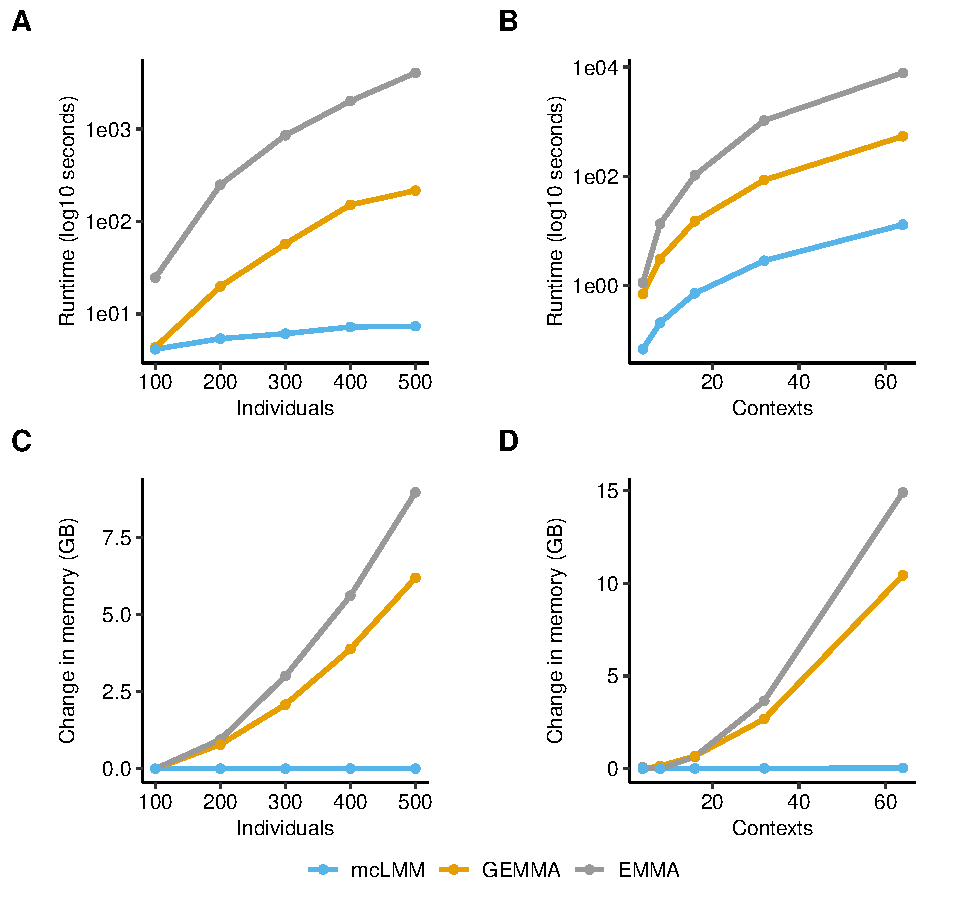
\includegraphics[width=0.75\textwidth]{chapter3/figures/Figure_1.pdf}
            \caption{Resource requirements of mcLMM, GEMMA, and EMMA across various simulated individual and context sizes with missing values (sampling rate of 0.5). For varying individuals, contexts were fixed at 50. For varying contexts, individuals were fixed at 500. (A-B) Runtime with log10(seconds) on the y-axis and number of individuals or contexts simulated on the x-axis. (C-D) Memory usage (GB) on the y-axis and number of individuals or contexts simulated on the x-axis. }
            \label{fig:fig1}
        \end{figure}
        
        In cases where there is no missing data, mcLMM allows for further speedups. We ran similar simulations to compare mcLMM with no missing data (optimal model) and mcLMM with missing data (iterative model). We observed a dramatic speedup, with sample sizes of 500,000 individuals across 10 contexts completed in under 10 seconds for the optimal model compared to around 15 minutes for the iterative model.
    
    \subsection{mcLMM enables powerful meta analyses to detect eQTLs}
        We utilized mcLMM to reduce the computational resource requirements of the Meta-Tissue pipeline, which fits a multiple-context LMM and combines the resulting effect sizes using METASOFT \cite{Sul}. While powerful, the existing approach utilizes EMMA to fit the LMM. For a recent release from the GTEx consortium  \cite{GTEx_Consortium2020-xx}, each pair of genes and single nucleotide polymorphisms (SNPs) required over two hours to run. Across hundreds of thousands of gene-SNP pairs, this method would require years of computational runtime to complete. Utilizing mcLMM, we were able to complete this analysis in 3 days parallelized over each chromosome. 
        
        We compared our approach to a method known as mash \cite{Urbut2019}. This approach utilizes effect sizes estimated within each context independently and employs a Bayesian approach to combine their results for meta-analysis. In order to estimate the power of these methods, we performed simulations as described in the methods. In null simulations, we observed well-controlled false positive rates at $\alpha = 0.05$ for mcLMM coupled with METASOFT. In our simulation with true positives, we observed an increased area under the receiver operating characteristic (AUROC) for mcLMM coupled with the random effects (RE2) METASOFT model compared to mash (Figure \ref{fig:fig2}).
        
        %% Figure 2 %%
        \begin{figure}
            \centering
            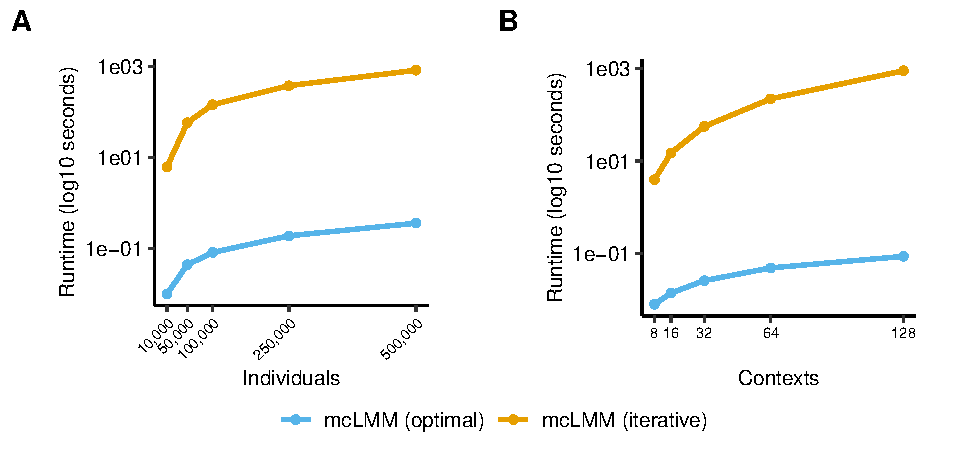
\includegraphics[width=\textwidth]{chapter3/figures/Figure_2.pdf}
            \caption{AUROC curves of mcLMM+METASOFT and mash in simulated data, assuming the effects of gene-SNP pairs are (A) shared and unstructured, and (B) shared and structured.}
            \label{fig:fig2}
        \end{figure}

        Next, we compared the number of significant associations identified in the GTEx dataset. The mash approach utilized gene-SNP effect sizes estimated by the GTEx consortium within each tissue independently. Concordant with our simulations, we observed that the Meta-Tissue approach, utilizing mcLMM for vast speedup, identified more significant eQTLs than mash (Figure \ref{fig:fig3}). These associations allow researchers to better understand the link between genetic variation and complex phenotypes through possible mediation of gene expression. 
        
        %% Figure 3 %%
        \begin{figure}
            \centering
            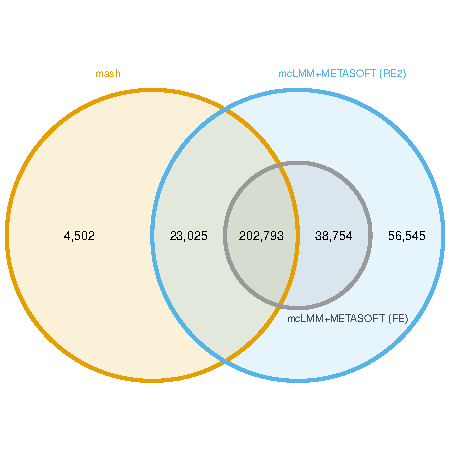
\includegraphics[width=0.75\textwidth]{chapter3/figures/Figure_3.pdf}
            \caption{Venn diagram of significant eQTLs identified by meta-analysis methods in the GTEx dataset. We compared mcLMM using two different models in METASOFT (RE2 and FE) to mash. Note that areas are not proportional to the number of eQTLs in each region. mcLMM+METASOFT (RE2) identified a total of 321,117 significant associations that contained 225,818 eQTLs identified by mash.}
            \label{fig:fig3}
        \end{figure}
        
    \subsection{mcLMM scales to millions of samples across related phenotypes}
        As a practical application of the efficiency of mcLMM, we performed a multiple phenotype GWAS in the UK Biobank. A multiple phenotype GWAS associates SNPs with several related phenotypes in order to increase the effective sample size for greater power, under the assumption that the phenotypes are significantly correlated. For our analysis, we combined HDL and LDL cholesterol, Apolipoprotein A and B, and triglyceride levels across 323,266 unrelated caucasian individuals in the UK Biobank. In total, 1,616,330 observations of these related phenotypes were fit as responses in the LMM. 
        
        The mcLMM approach completed this analysis over 211,642 SNPs with an additional 14 covariates, parallelized over each chromosome, within a day. Each chromosome was analyzed on a single core machine with 32 GB of memory, with each test taking around 2 seconds to complete. We identified several significant loci, a subset of which replicate previous findings for specific phenotypes included in the model, such as HDL cholesterol \cite{Wojcik} (Figure \ref{fig:fig4}). Existing approaches, namely EMMA and GEMMA, require orders of magnitude more memory to begin this analyses and could not be run on the available computational resources.
        
        %% Figure 4 %%
        \begin{figure}
            \centering
            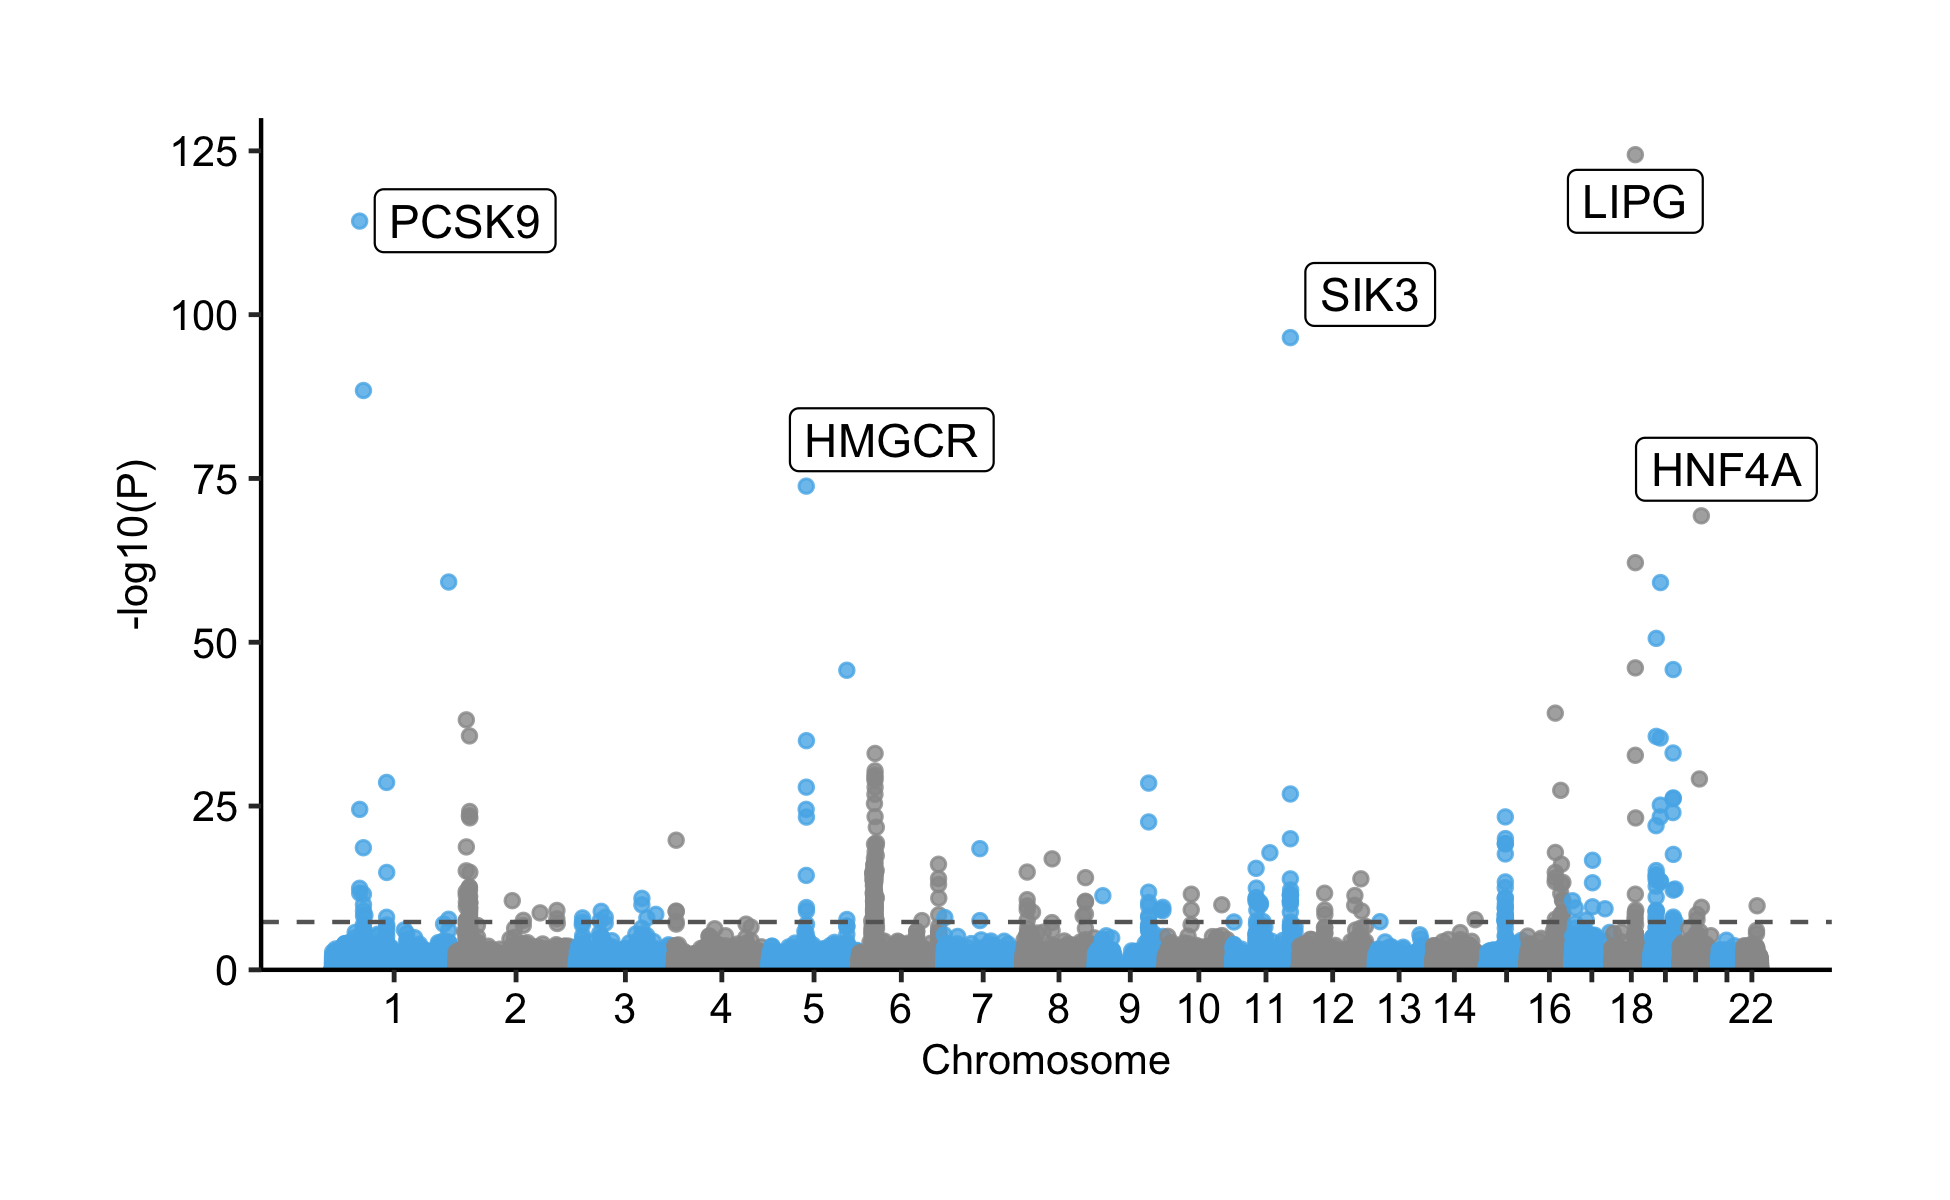
\includegraphics[width=\textwidth]{chapter3/figures/Figure_4.png}
            \caption{Multiple phenotype GWAS results from UK Biobank. Five phenotypes (LDL cholesterol, HDL cholesterol, Apolipoprotein A, Apolipoprotein B, and triglyceride levels) were used as responses in the mcLMM framework. The model was fit with 1,616,330 observations from 323,266 unrelated Caucasian individuals. In total, 211,642 SNPs were tested with an additional 14 covariates. Each test required around 2 seconds to run on a 32GB machine and was parallelized over each chromosome. The -log10 of the p-values are plot on the y-axis and genomic positions on the x-axis. The horizontal dashed line indicates the genome wide significance level at $p=0.05/1e6$. The top hit for 5 different chromosomes is annotated with the gene containing the SNP. These genes have been previously identified as associated with a subset of these phenotypes.}
            \label{fig:fig4}
        \end{figure}
\section{Discussion}

    We presented mcLMM, an efficient method for fitting LMMs used for multiple context association studies. Our method provides exact results and scales linearly in time and memory with respect to sample size, while existing methods are cubic. This efficiency allows mcLMM to process millions of samples over several contexts within a day on minimal computational resources, as we showed in simulation and in the UK Biobank. The association parameters learned by mcLMM can further be utilized with the METASOFT framework to provide powerful meta-analysis of the associations, as we showed in the GTEx dataset. 
    
    Previous work has observed the potential speedup to linear complexity for LMMs when the matrix $K$ is approximated with a low rank representation \cite{Lippert2011}. Here, we optimize the method specifically for the low rank matrix that arises naturally in multiple context association studies, allowing our method to provide exact results and scale to hundreds of thousands of samples with minimal computational resources.                         % etc.
%\chapter{Selection contributes to skewed X chromosome inactivation across human tissues}

\section{Background}
X chromosome inactivation (XCI) occurs in blastocysts during embryonic development. Under no external pressures, the process is assumed to be random and is established in about a dozen cells and all daughter cells will inherit the XCI status of these cells \cite{Takagi1975-es}. Skew in XCI has been widely observed in female mammals and is accepted to be common across individuals \cite{Shvetsova2019-re}. Selective pressures have been implicated in contributing to XCI skew, especially in the context of diseases such as cancer \cite{Brown1999-dc,Migeon1998-gc}. In addition, XCI skew was found to be heritable and correlated with age based on a twin study \cite{Zito2019-hu}. Recent work argued that observed XCI skew in the general female population is the result of expected randomness in early development \cite{Shvetsova2019-re}. 

Here, we show that XCI skew in a general female population in the GTEx dataset \cite{GTEx_Consortium2020-xx} is associated with genetic scores related to deleteriousness and proliferative potential. We hypothesize that differences in the fitness of maternal and paternal X chromosomes may contribute to skewed XCI across tissues into adulthood (Figure \ref{fig:fig4.1}a).  Furthermore, we perform a scan of common variants across the X chromosome to identify specific loci associated with overall XCI skew in these individuals.

\begin{figure}[ht]
    \centering
    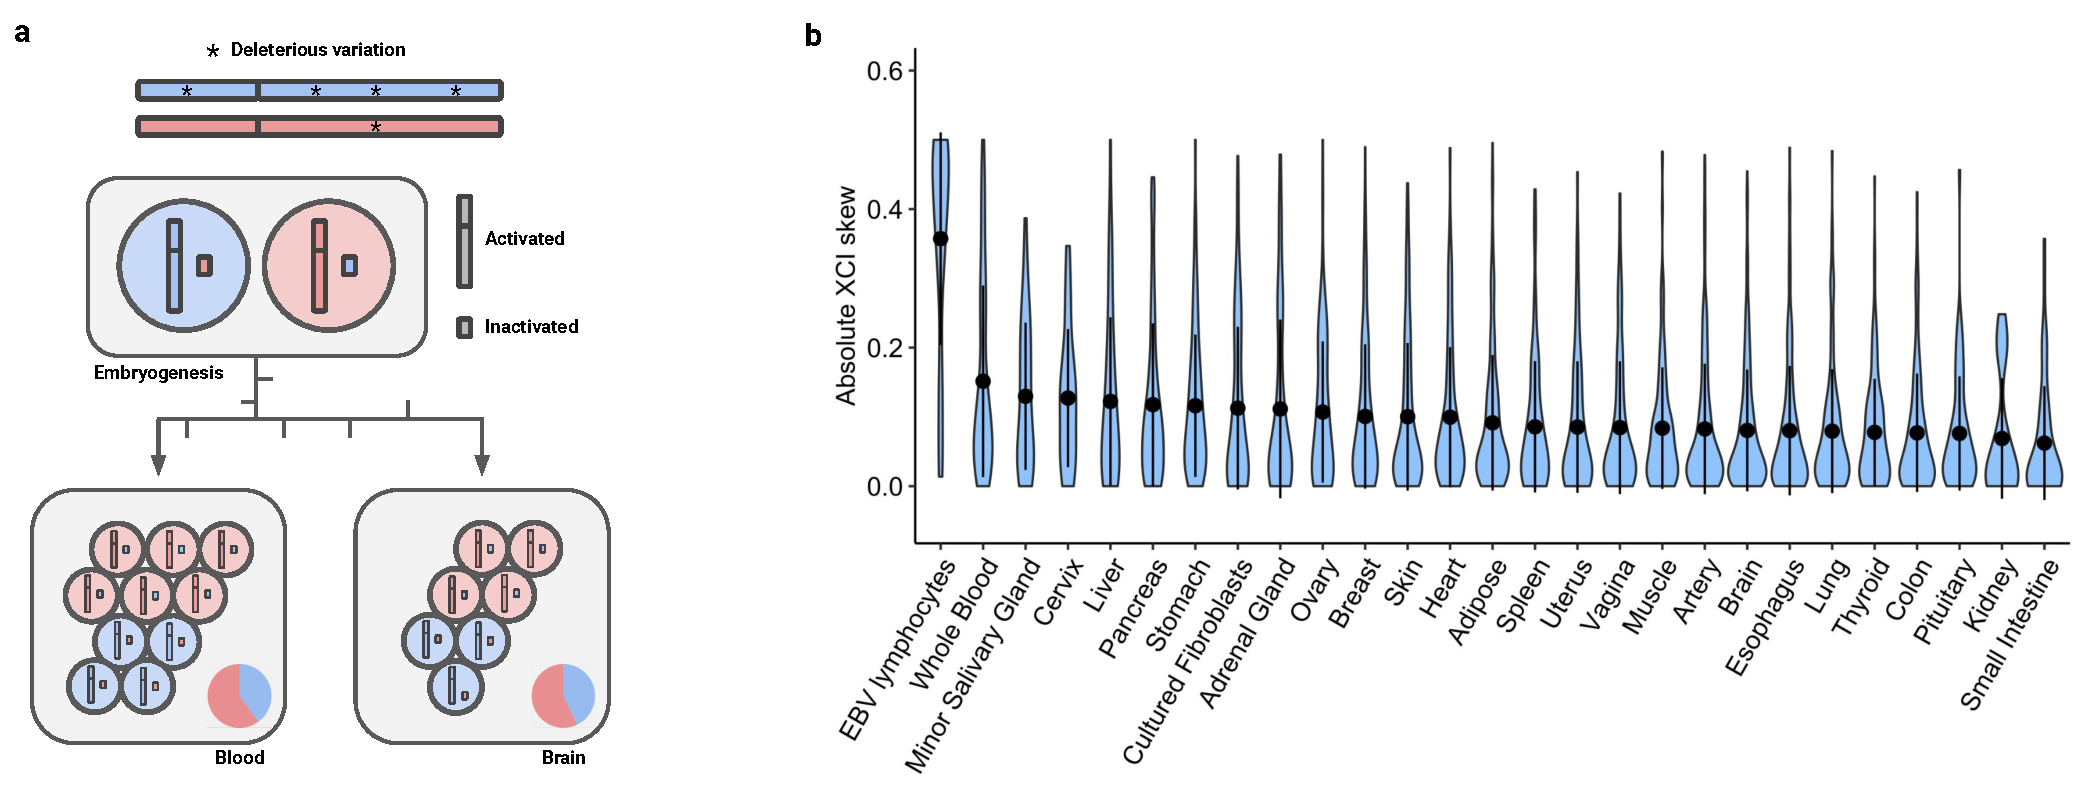
\includegraphics[width=\textwidth]{chapter4/Figures/Figure_1.pdf}
    \caption{
        Measuring XCI skew across tissues 
        \textbf{a}, Schematic overview of selection hypothesis. An individual inherits one haplotype (red) that is more fit than the other (blue) due to genetic variation. Given equal population sizes in embryonic development, we hypothesize that fitness differences will produce skewed populations in fully developed tissues.
        \textbf{b}, Violin plot of absolute XCI skew on the y-axis. Tissues are sorted by mean on the x-axis. Dots indicate mean of the absolute skew with vertical lines indicating one standard deviation.}
    \label{fig:fig4.1}
\end{figure}

\section{Methods}
\subsection{Transcriptomic and genetic data}

The following data were processed and made available by the GTEx consortium \cite{GTEx_Consortium2020-xx}. GENCODE v26 and the GRCh38 human reference genome was used to process both WGS and RNA-seq data. RNA-seq data was aligned using STAR with WASP filtering. Allele-specific read counts at heterozygous sites were quantified with GATK ASEReadCounter. Genetic variants were called from whole genome sequencing data and phased with read-aware SHAPEIT2. All analyses were restricted to caucasian samples. 

\subsection{Quantifying XCI skew}

Allele-specific read counts were matched to haplotypes from the phased WGS data. Only heterozygous sites within fully inactivated genes reported by Carrel and Willard \cite{Carrel2005-zm} and Cotton et al \cite{Cotton2013-jl} were considered. Furthermore, we restricted to genes where no females were observed to escape inactivation in Cotten et al. LiftOver (https://genome.ucsc.edu/cgi-bin/hgLiftOver) was used to convert these reported gene windows from GRCh37 to GRCh38 positions. Moreover, we only considered variants that had at least 10 overlapping reads. XCI skew was calculated at each heterozygous site in the gene windows as the number of reads coming from haplotype 1 divided by the total number of reads at the site. The final XCI skew measurement for each sample was the median of these per-site observations. In addition, since haplotypes are not readily distinguishable as maternal or paternal, we also calculated the absolute XCI skew as the absolute deviation of this value from 0.5. 

We also calculated skew in the same manner in autosomes. Specifically, if $m$ heterozygous sites were used to calculate XCI in a sample, we randomly selected $m$ heterozygous sites with at least 10 overlapping RNA-seq reads on the q-arm of each non-acrocentric autosome. We used these sites to calculate skew for each autosome. 

\subsection{Genetic score association}

Four scores were defined to measure genetic burden of X chromosome haplotypes in females. First, we considered the difference in average CADD score \cite{Rentzsch2019-pk} between the two haplotypes. A higher CADD score corresponds to an increased likelihood of deleteriousness. CADD Phred scores were retrieved using VEP \cite{McLaren2016-jd}. The CADD score associated with each alternate allele on each haplotype was averaged. The remaining scores were proportions of different types of mutations carried by a haplotype. We considered the proportion of alternate alleles, missense mutations, and synonymous mutations carried by a haplotype. This proportion is calculated as the count of the variant-type on one haplotype divided by the total number of these variants found across both haplotypes. Annotations indicating the coding consequence of variants were obtained using VEP.

We associated these scores with XCI skew using a linear mixed model. Specifically, we used the lmer function from the lmerTest package \cite{Kuznetsova2017-jp} to fit the following model across all tissues, where the (1\textbar Grouping) notation indicates a random intercept for the specified grouping:
\begin{equation}
\text{H1 XCI Skew} \sim \text{H1 Burden + Age + (1\textbar Individual) + (1\textbar Tissue)}
\end{equation}
In this model, we include random intercepts for the individual and tissue of origin for each sample. The significance of these associations were determined using a one-sided t-test, under the assumption that increased burden will decrease skewing towards a haplotype.

Blood-related polygenic scores were retrieved from PGS Catalog \cite{Lambert2021-iu}. We used scores for the following cell counts: platelet (PGS000186), red blood cell (PGS000187), basophil (PGS000163), neutrophil (PGS000182), eosinophil (PGS000165), monocyte (PGS000177), and lymphocyte (PGS000172) \cite{Vuckovic2020-gf}. GRCh38 positions of the variants used for these scores were retrieved from SNP Nexus \cite{Oscanoa2020-ac}. We calculated each polygenic score for both haplotypes and modeled the difference in scores as follows:
\begin{equation}
\text{H1 XCI Skew} \sim \text{(H1 PGS - H2 PGS) + Age + (1\textbar Individual) + (1\textbar Tissue)}
\end{equation}
The significance of these associations were determined by using a one-sided t-test, under the assumption that increased proliferative potential will increase skewing towards a haplotype. 

Each of these tests were also performed for autosomes as controls with the following model:

\begin{align}
\begin{split}
\text{H1 XCI Skew} \sim & \text{ (H1 PGS - H2 PGS) + Age +} \\
                        & \text{ (1\textbar Individual) + (1\textbar Tissue) + (1\textbar Chromosome)}
\end{split}
\end{align}
where “Chromosome” refers to the autosome used to calculate skew. A Bonferroni-corrected significance threshold of 0.05/8 was used for the 4 burden scores and 0.05/14 was used for the 7 blood-related polygenic scores. 

\subsection{Identifying significant XCI loci}

The phased X chromosome variants were filtered with PLINK 2 \cite{PLINK2}. SNPs were extracted with a minor allele frequency threshold of 0.01 and Hardy-Weinberg equilibrium p-value threshold of 1e-6. LD pruning was performed with a window size of 100 kilobases, step size of 5 variants, and $r^2$ threshold of 0.5. 

These filtered variants were marginally tested in a linear mixed model to measure association with absolute XCI skew. We fit the following linear mixed model:
\begin{equation}
\text{Absolute XCI Skew} \sim \text{Heterozygous + Age + (1\textbar Individual) + (1\textbar Tissue)}
\end{equation}
where Heterozygous is 1 if the sample is heterozygous for the variant and 0 if the sample is homozygous. We modeled absolute skewing under the assumption that heterozygosity will lead to differences in fitness and consequently increased overall skewing. Given this assumption, we determined the significance of these associations using a one-sided t-test under this hypothesis. The resulting p-values were converted to q-values \cite{Storey2003-kx} and considered significant using a threshold corresponding to a 0.05 local false discovery rate.

At the two significant loci, this linear mixed model was also used to determine the significance of the difference in skewing between homozygous samples and groups defined by the phasing of the variant in heterozygous individuals. For these associations, we fit the following model separately for individuals with the variant on H1 and on H2:
\begin{equation}
\text{H1 XCI Skew} \sim \text{Heterozygous + Age + (1\textbar Individual) + (1\textbar Tissue)}
\end{equation}
Since we do not assume the direction of individual variant effects on XCI skewing, we performed a two-sided t-test to determine significance of these associations. 

\subsection{Associating XCI-linked genetics in males}

To address the possibility that the burden and proliferation scores are capturing regulatory effects, such as downregulation of a haplotype rather than increased inactivation, we calculated these scores within males. Like in the female samples, we utilized variants outside of the fully inactivated genes used to calculate skew. Given that males have one X chromosome, we associated these scores with the expression of each gene on the X chromosome. We fit a model similar to those used for identifying expression quantitative trait loci. Specifically, we performed a linear regression within each tissue independently, correcting for the top 5 genetic principal components, PCR, and platform. We also corrected for PEER factors, \cite{Stegle2012-uf} using 15 for sample sizes less than 150 and adding an additional 15 factors for each 100 samples. The resulting p-values from the linear regression were converted to q-values \cite{Storey2003-kx} and considered significant at a local false discovery rate threshold of 0.05. 

\section{Results}

\subsection{Estimating XCI skew from RNA-seq data}

We analyzed data generated by the GTEx consortium \cite{GTEx_Consortium2020-xx}, which included RNA-seq and phased whole genome sequencing data measured across 243 caucasian female samples and 472 caucasian male samples. We measured XCI skew in females as the difference in expression measured from each X chromosome in an RNA-seq experiment. Since XCI does not completely silence the entire X chromosome, we restricted our analysis to genes that have been previously observed to be fully inactivated \cite{Carrel2005-zm,Cotton2013-jl,Tukiainen2017-xm}. Read counts at heterozygous sites in these regions were assigned to haplotypes determined with phased whole genome sequencing data. The skew in RNA-seq reads was calculated at each site as the number of reads coming from one haplotype divided by the total number of reads. XCI skew for a sample was calculated as the median of these values. A median of 45 heterozygous sites were used for this calculation across the samples (Figure \ref{fig:supp_fig4.1}). We observed variability in XCI skew across tissues, with EBV-transformed lymphocytes exhibiting nearly complete skew in many samples (Figure \ref{fig:fig4.1}b).  Given this extreme skewing likely due to culture conditions, we removed these samples from downstream analyses. Furthermore, we observed correlation of XCI skew across the different tissues (Figure \ref{fig:supp_fig4.2}).

\begin{figure}[ht]
    \centering
    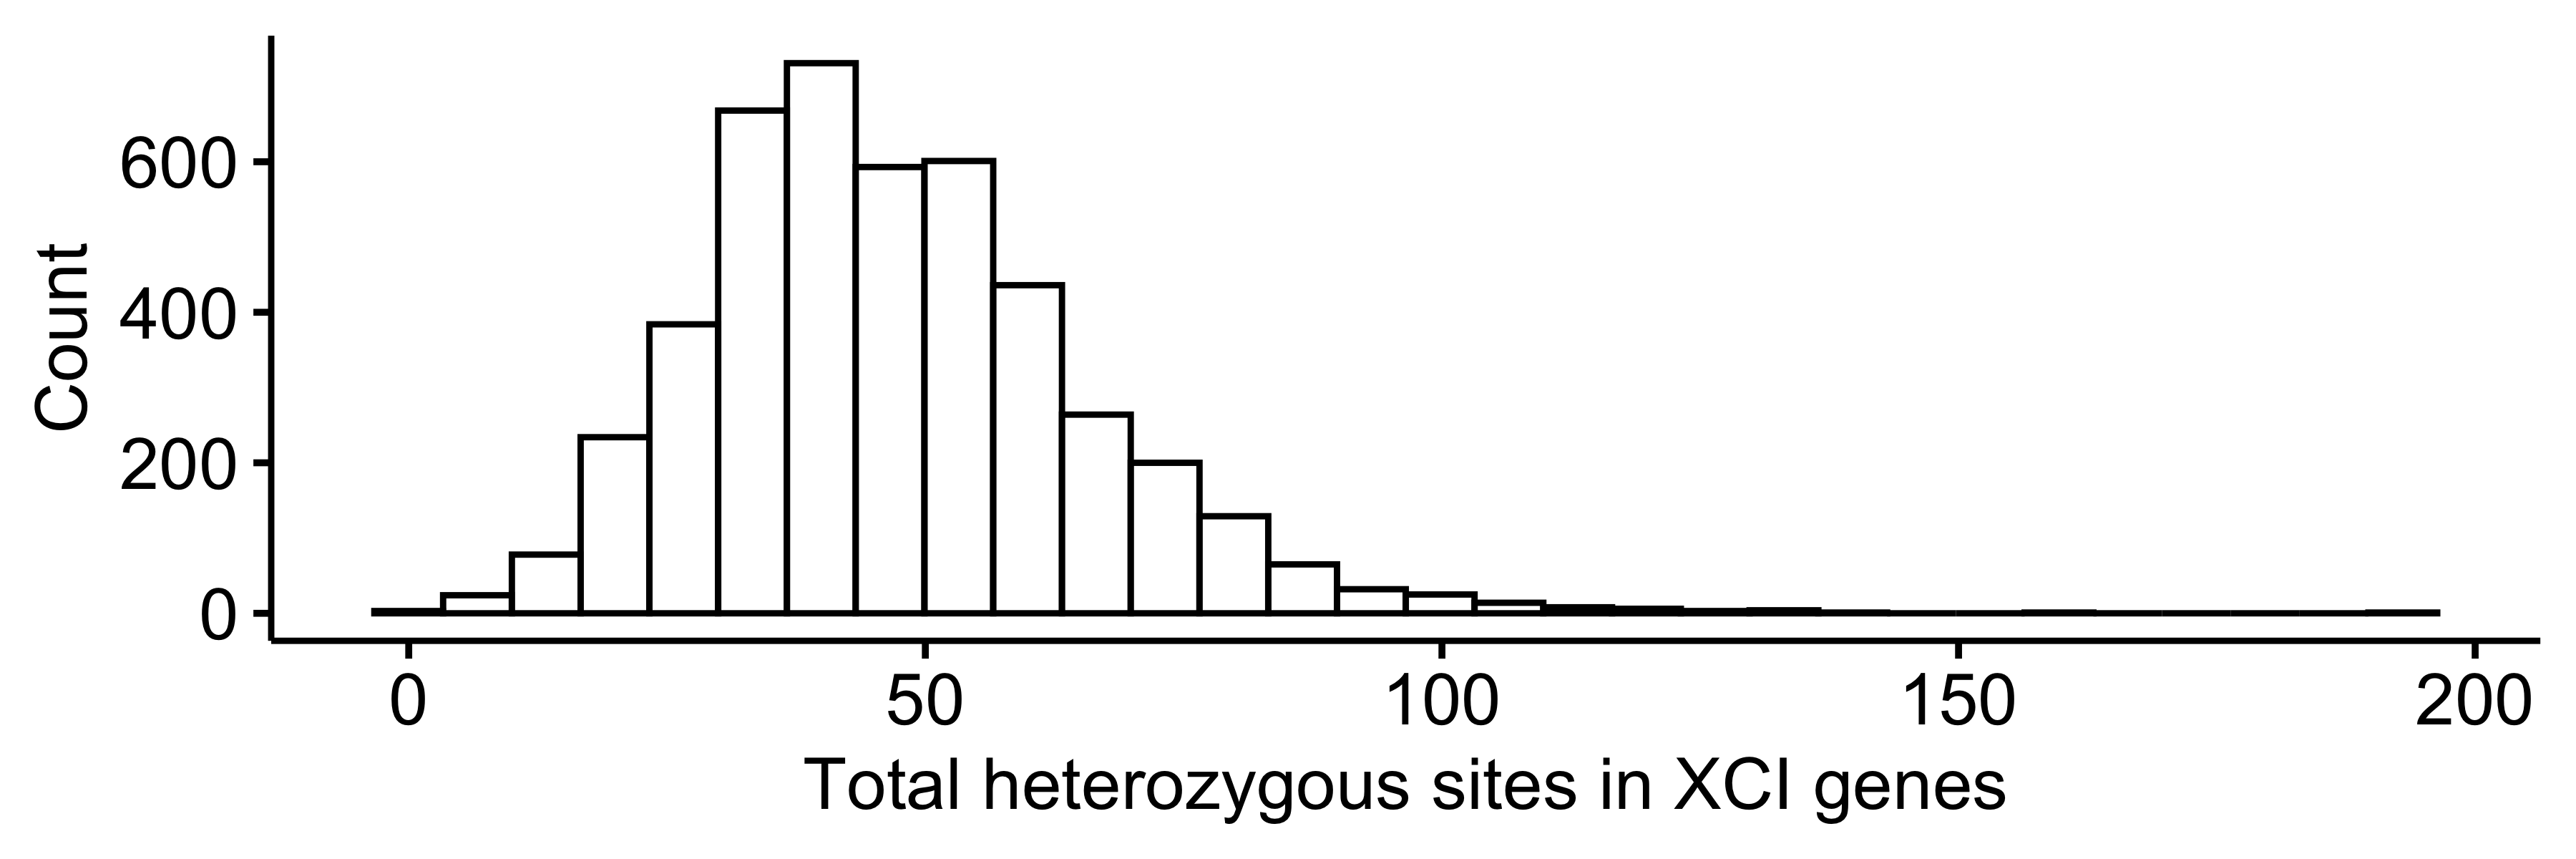
\includegraphics[width=0.75\textwidth]{chapter4/Figures/Supplementary_Figure_1.png}
    \caption{
        Histogram of number of heterozygous sites with coverage of 10 or more RNA-seq reads and within fully inactivated genes used to calculate XCI skew for each sample. We observed a mean of 46.805 and median of 45 variants used to calculate skew (the median of per-site skew). 
    }
    \label{fig:supp_fig4.1}
\end{figure}
\begin{figure}[ht!]
    \centering
    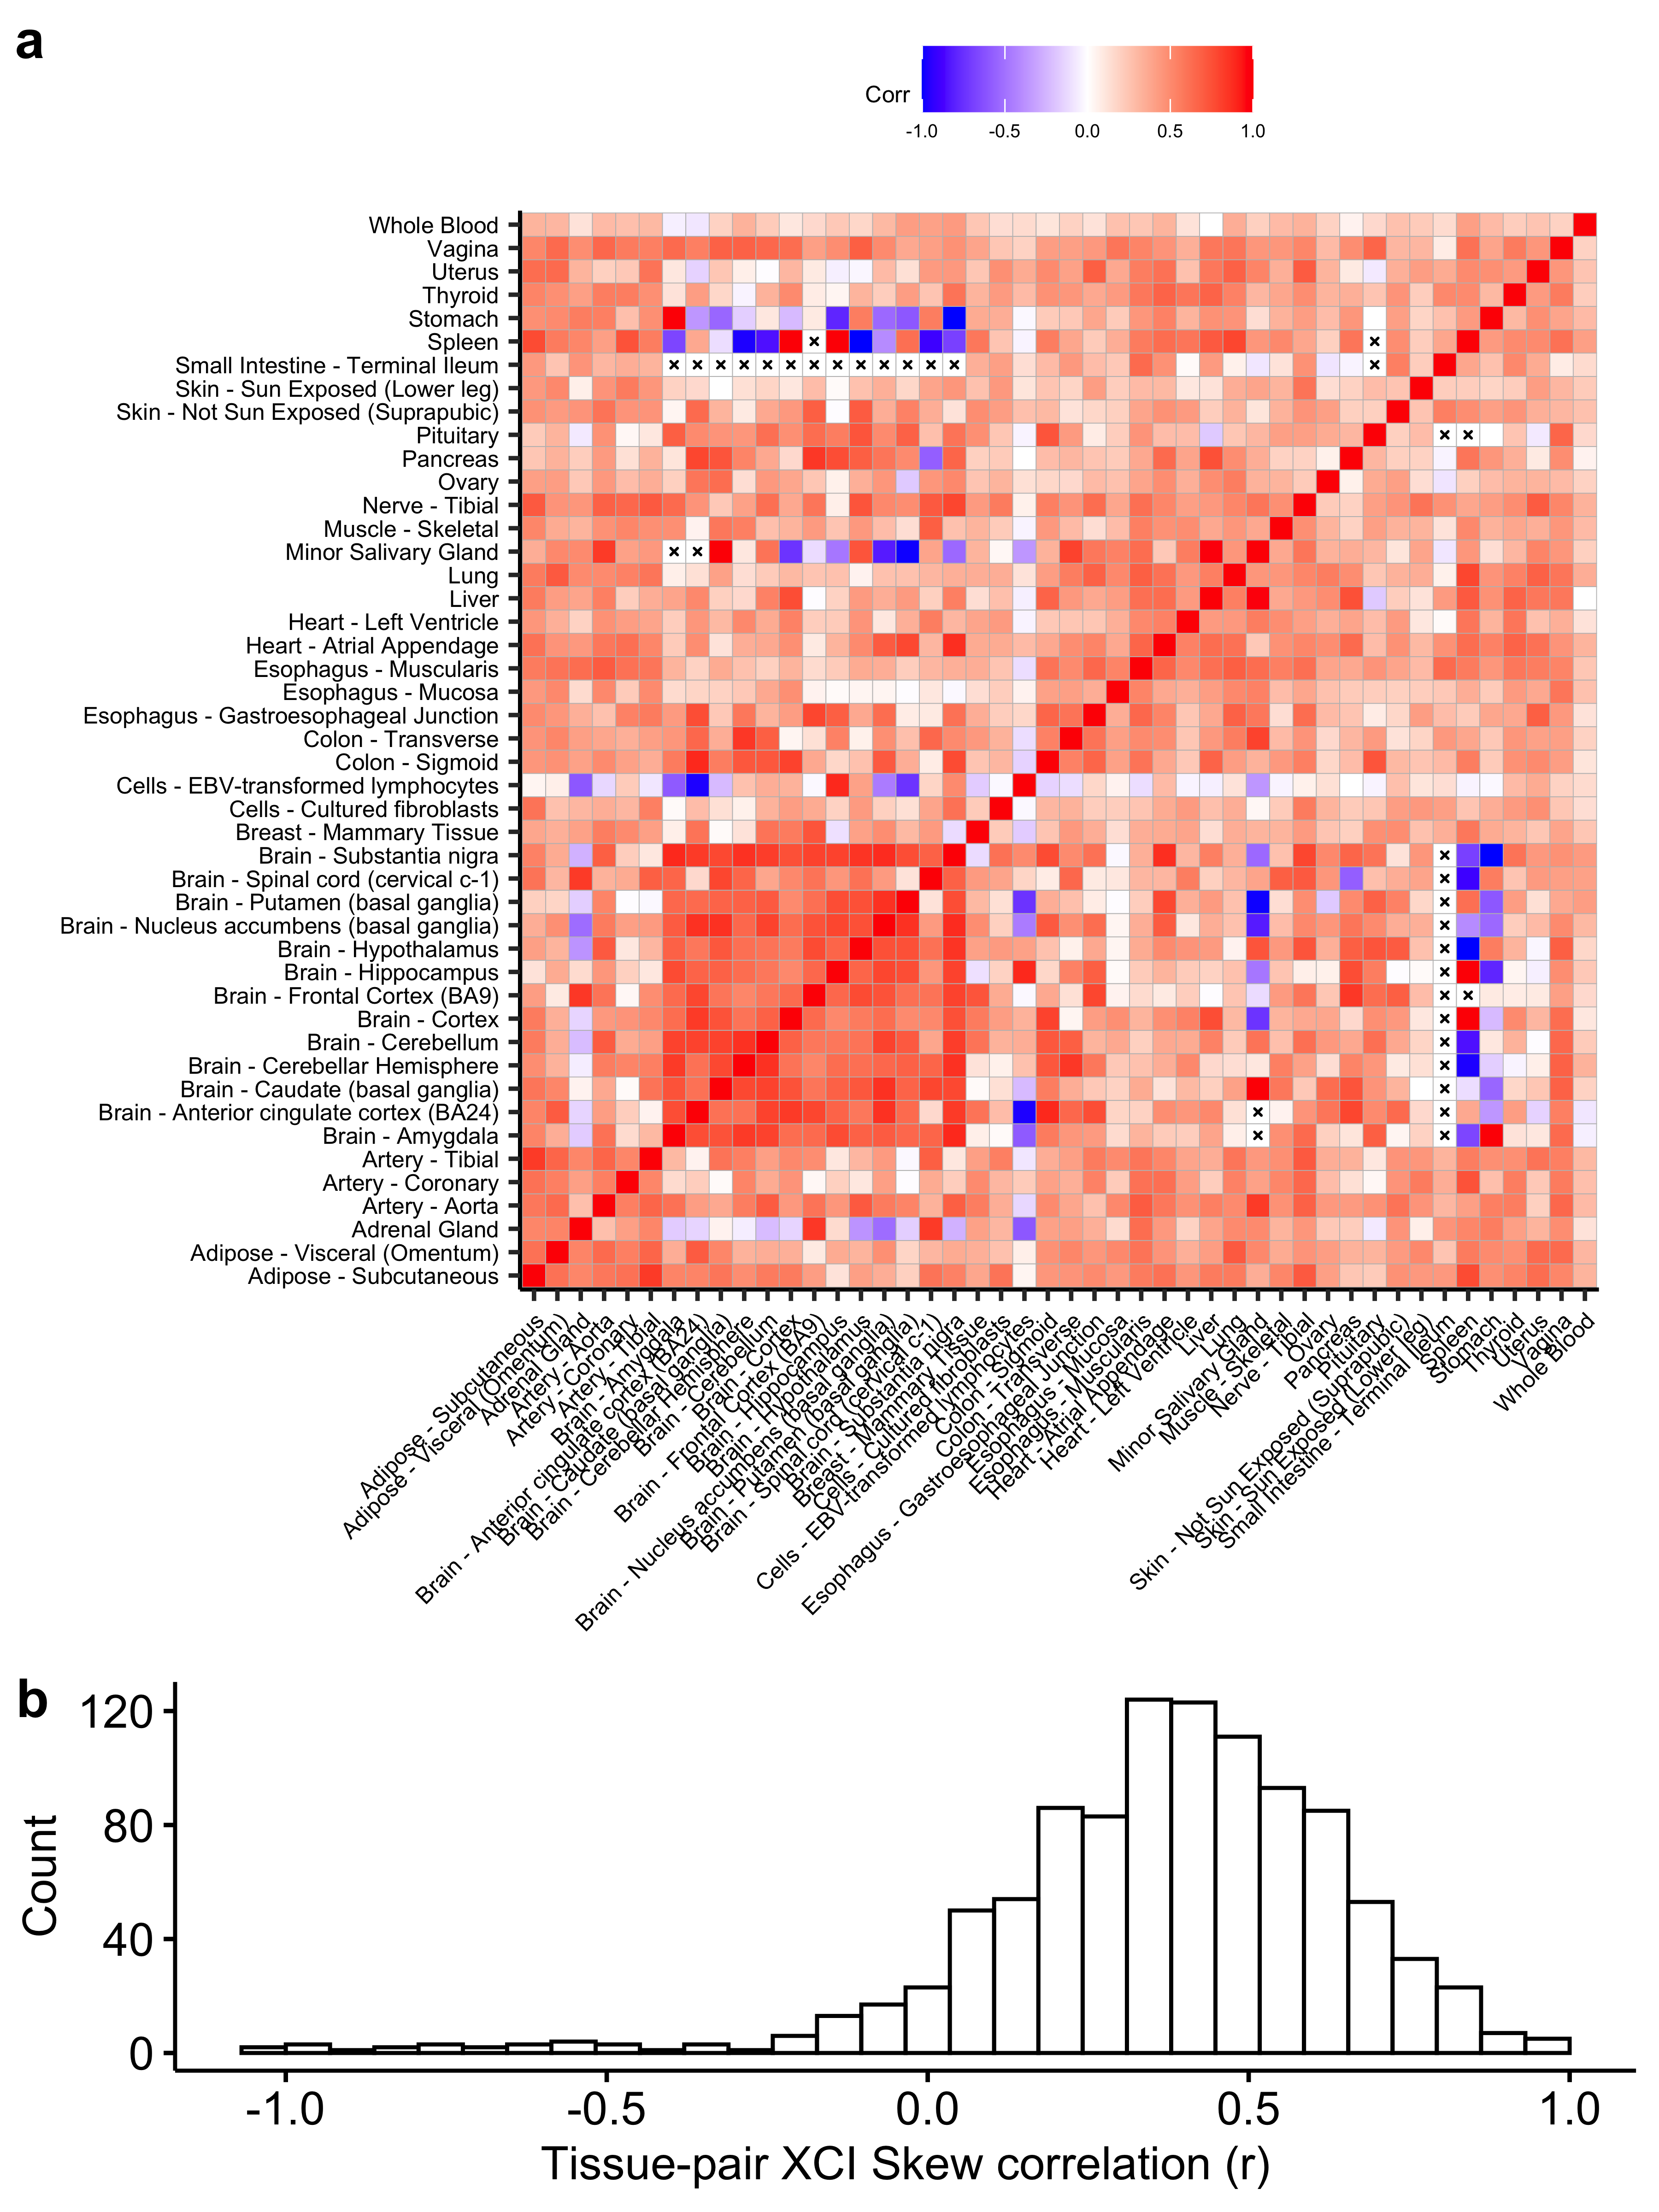
\includegraphics[width=0.75\textwidth]{chapter4/Figures/Supplementary_Figure_2.png}
    \caption{
        Pearson correlation of XCI skew between tissues.
        \textbf{a}, Correlation matrix of tissue-specific XCI skew. White boxes with 'X' symbol indicate that less than 25 observations were available for the tissue pair.
        \textbf{b}, Histogram of correlation between 1,017 non-identical tissue pairs. We observed a mean correlation of 0.3663 and median of 0.3992.
    }
    \label{fig:supp_fig4.2}
\end{figure}

Inferring XCI skew from expression data can be confounded by both technological and biological factors that may lead to similar associations with our genetic burden scores. Reference bias, the tendency for RNA-seq reads with reference alleles to better map to a reference genome than non-reference alleles \cite{Stevenson2013-cg}, may be a significant confounding variable. This bias is especially relevant to the genetic burden defined by the proportion of alternate alleles carried by a haplotype. For example, an alternate allele may have lower observed expression than the reference allele simply due to reference bias rather than XCI skew. To account for this source of bias, we utilized RNA-seq reads that were aligned with a filter utilizing WASP, a method that accounts for reference bias by mapping reads with swapped genotypes \cite{Van_de_Geijn2015-oy}.
Regulatory effects of genetic variation may also lead to imbalances in expression measured from each X chromosome that may be erroneously attributed to skew in X chromosome inactivation. To address this source of confounding, we performed similar experiments using the non-acrocentric autosomes (chromosomes with arms of roughly equal size) of the female samples. In short, we calculated skewing at heterozygous sites that were captured by RNA-seq reads on the q or long arm of the autosome. We observed no significant level of average ‘skewing’ in these chromosomes (Figure \ref{fig:supp_fig4.3}). 

\begin{figure}[ht]
    \centering
    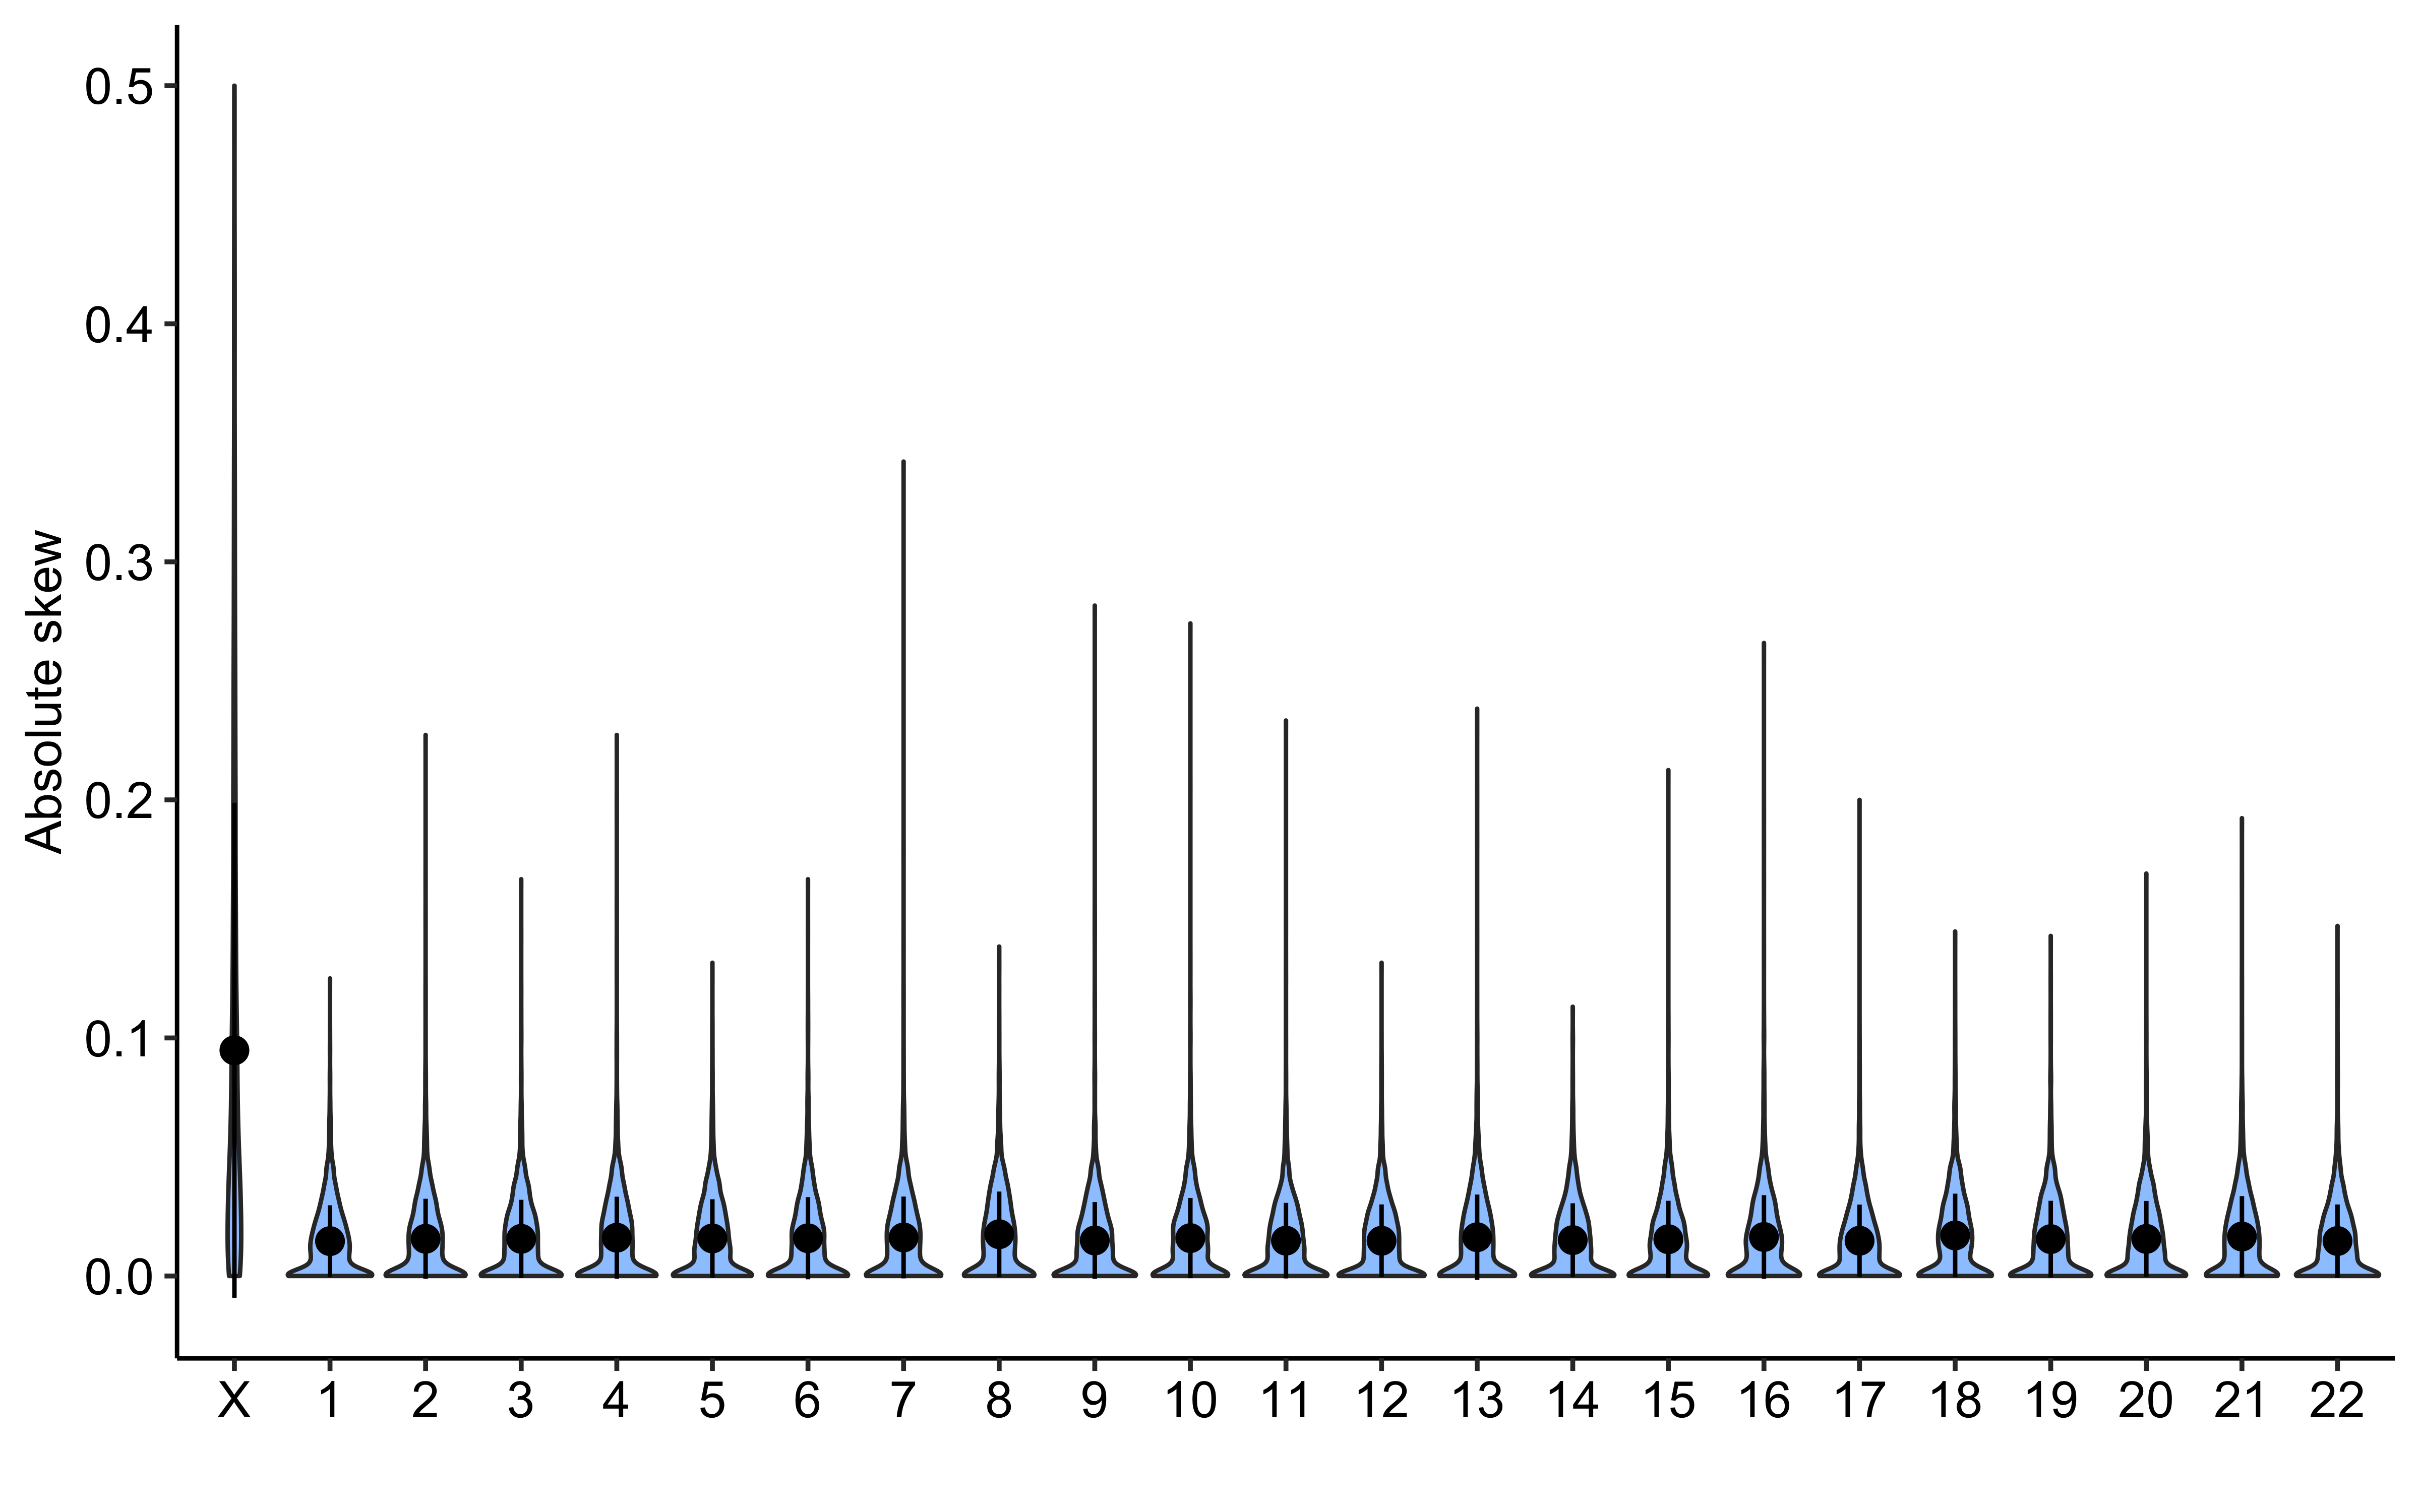
\includegraphics[width=0.75\textwidth]{chapter4/Figures/Supplementary_Figure_3.png}
    \caption{
        Estimated absolute skew in expression at heterozygous sites on the X chromosome and non-acrocentric autosomes. On the X chromosome, this value is used as the estimate of inactivation skewing since heterozygous sites are within fully inactivated genes. On the autosomes, an equal number of heterozygous sites used on the X chromosome for each sample were randomly selected from the q-arm to estimate the median skew in expression. Dots indicate mean of absolute skew with vertical lines indicating one standard deviation.
    }
    \label{fig:supp_fig4.3}
\end{figure}

We also performed an analysis of the male GTEx samples to test the possibility of regulatory effects rather than skewing in inactivation. Since males only have one X chromosome, we associated genetic features with expression of each gene on the X chromosome. If our genetic scores are associated with downregulation of expression rather than cause XCI skew, we anticipated this experiment to show a significant negative association with the expression of X chromosome genes across males.

\subsection{Genetic burden is associated with XCI skew}

We defined the following genetic burden scores for this analysis: the proportion of missense and synonymous mutations carried by each haplotype, and the difference in average CADD score \cite{Rentzsch2019-pk} between the two haplotypes. CADD scores provide a quantitative measure of the predicted deleteriousness of a variant. Only genetic variation outside of the genes that were used to calculate XCI skew were considered in these scores to avoid capturing cis regulatory effects. To associate these burden measures with XCI skew, we fit a linear mixed model with random intercepts accounting for the individual of origin for each tissue sample and tissue type. In this model, the difference in CADD score between haplotypes had a significant negative effect on XCI skew (coefficient = -0.1289 ± 0.0451, p = 0.0023) (Figure \ref{fig:fig4.2}a). This result suggests that a higher genetic burden in terms of deleterious variation is associated with higher rates of inactivation of the haplotype. We found that this association was not significant across the non-acrocentric autosomes (Table \ref{table:table4.1}). In addition, these burden scores were not associated with the regulation of gene expression on the X chromosome in male samples. 

\begin{figure}[ht]
    \centering
    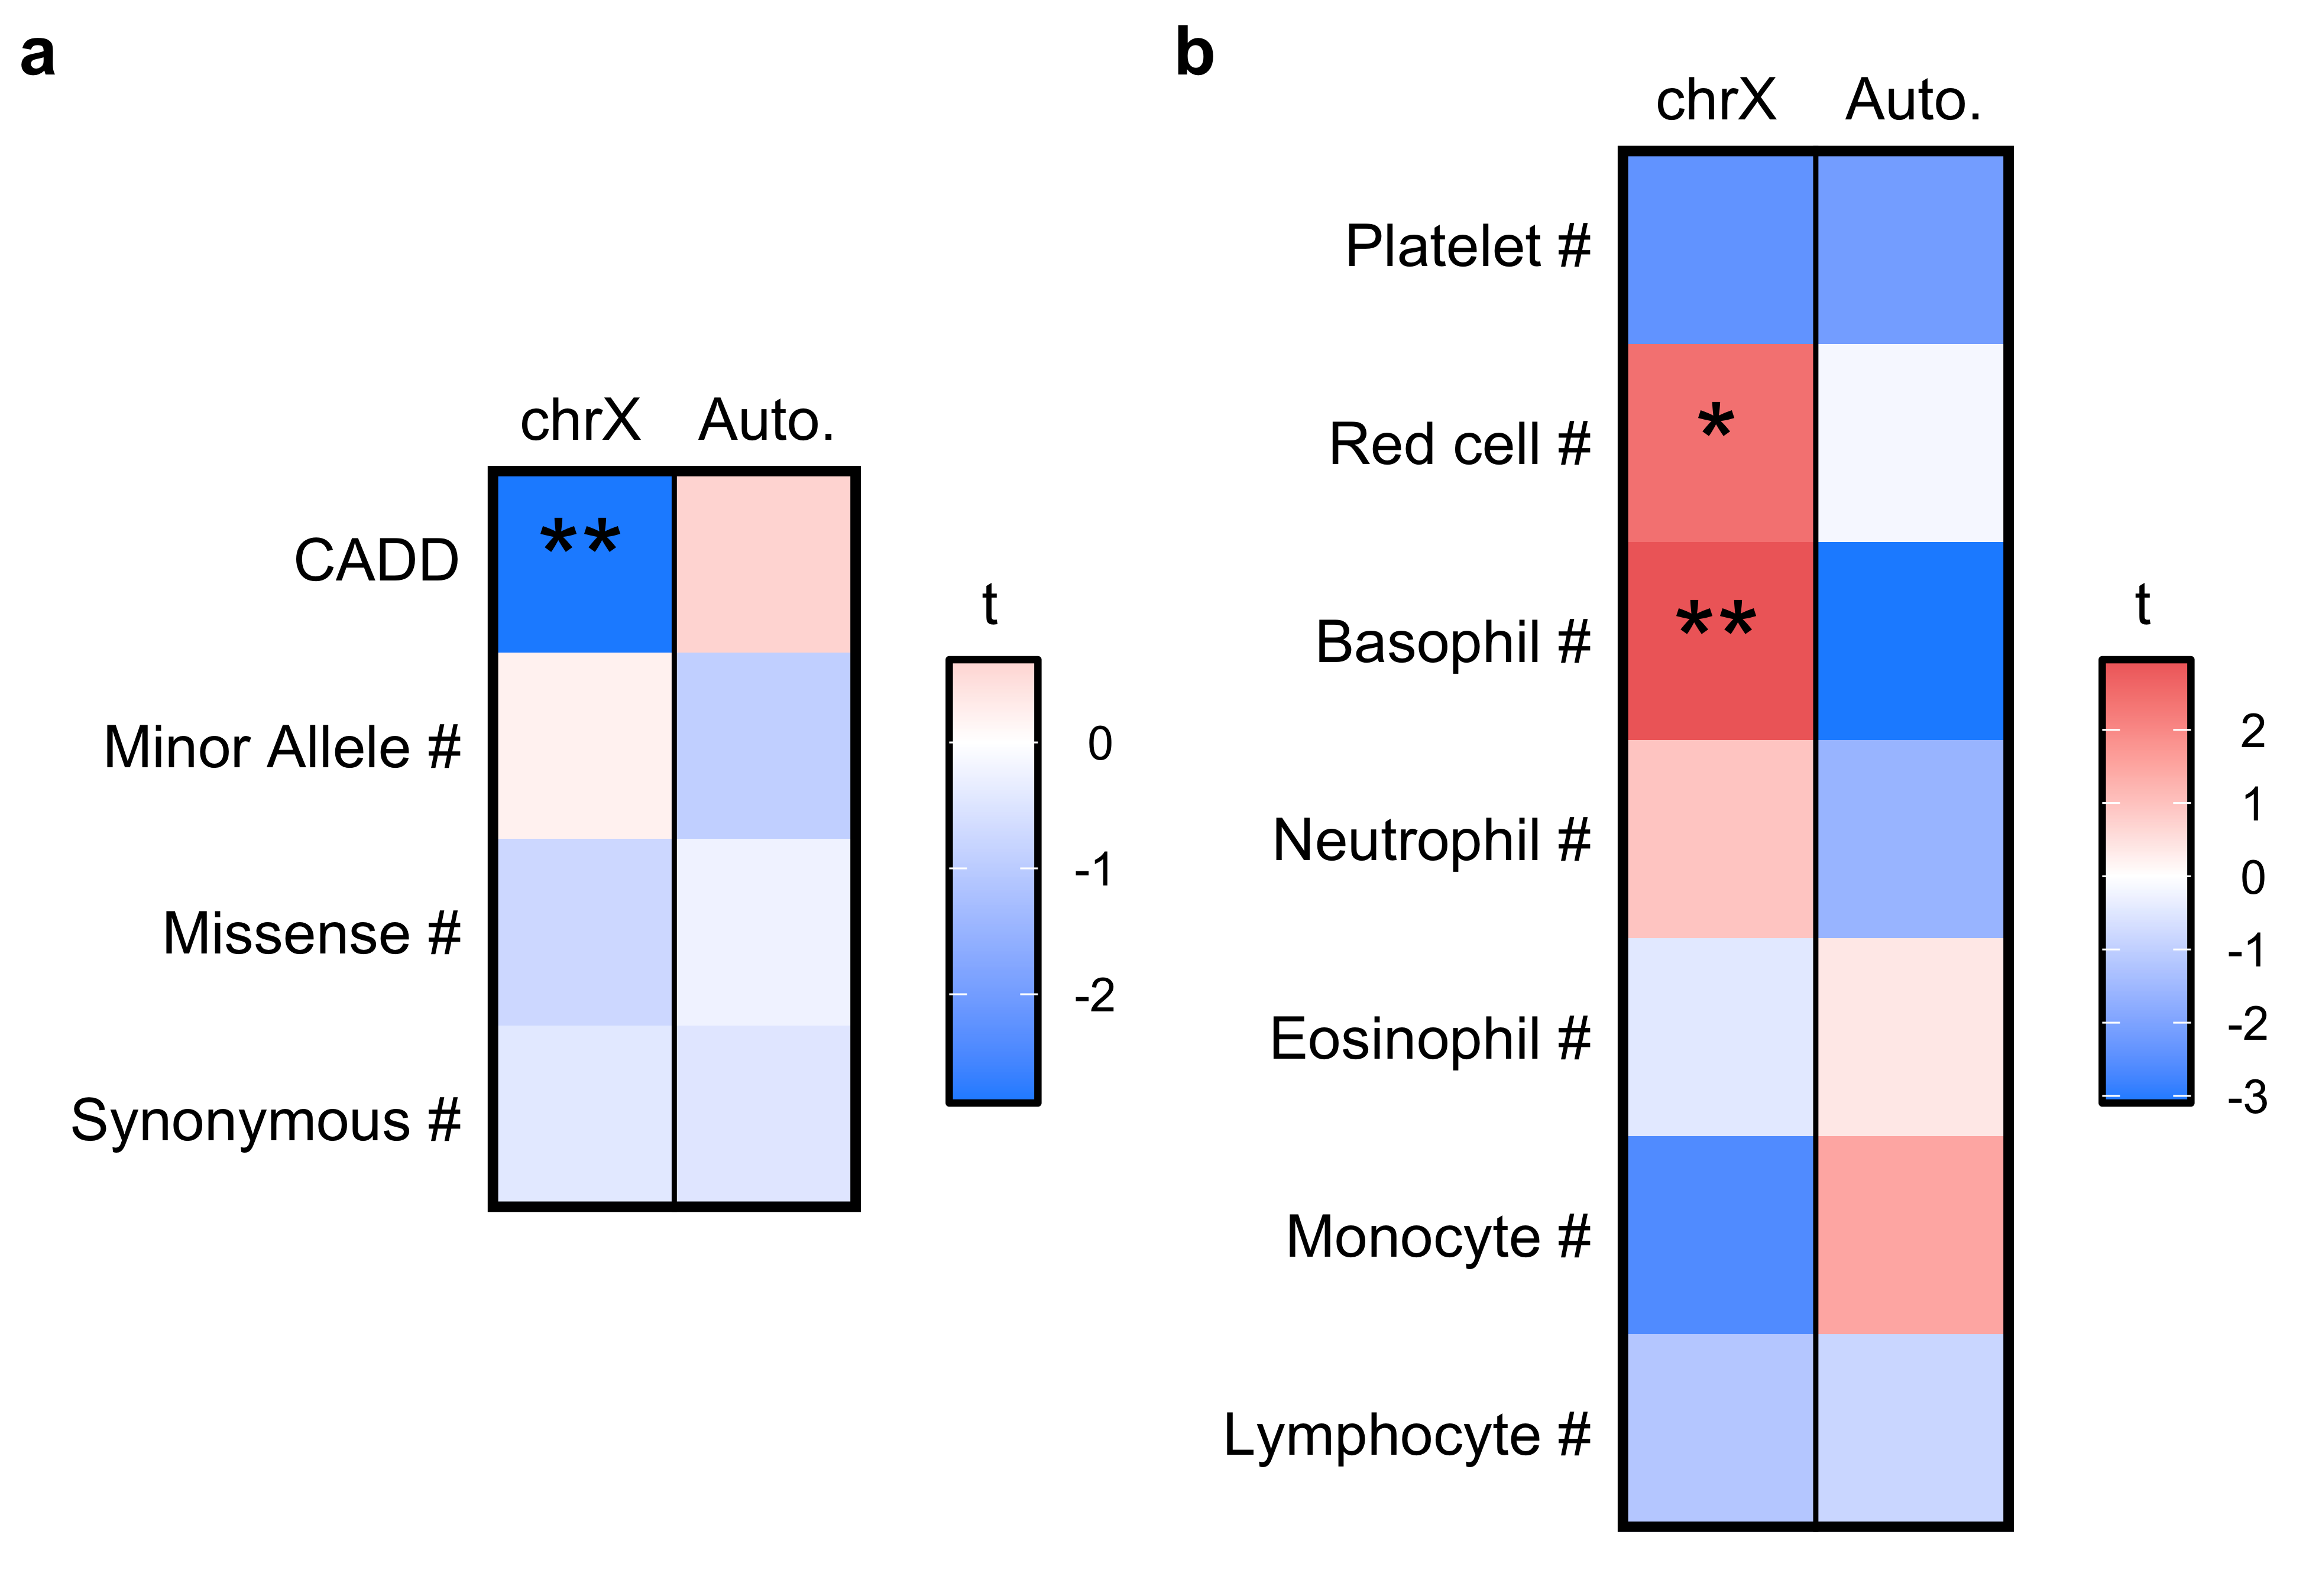
\includegraphics[width=0.5\textwidth]{chapter4/Figures/Figure_2.png}
    \caption{
        Association between genetic scores and skew estimated from expression at heterozygous sites on X chromosome (chrX) and non-acrocentric autosomes (Auto.). Colors indicate the relative t-score from a linear mixed model association test with an asterisks (*) indicating significance at $\alpha=0.05$ and double asterisks (**) indicating significance after Bonferroni correction.
        \textbf{a}, Association results of genetic burden scores with estimated skew. A one-sided t-test was performed under the assumption that increased genetic burden decreases skew towards the haplotype. CADD indicates difference in mean CADD score of each haplotype. The remaining scores compare the number of the indicated mutations on each haplotype.
        \textbf{b}, Association results of proliferative polygenic scores with estimated skew. Counts of different blood cell types were used as a proxy for proliferative potential. A one-sided t-test was performed under the assumption that increased proliferation genetic scores will increase skew towards the haplotype.}
    \label{fig:fig4.2}
\end{figure}
\begin{table}[ht]
\scriptsize
\caption{Burden associations with skewing in XCI and autosomal q-arm expression}
\centering
\begin{tabular}{llllll}
  \hline
 Burden Score & Chromosome(s) & $\beta$ (s.e.) & df & $t$ & $P$ \\ 
  \hline
CADD & chrX & -0.1289 (0.0451) & 240.6684 & -2.8579 & 0.0023 \\ 
   & Auto. & 0.0024 (0.0037) & 60762.2663 & 0.6516 & 0.7427 \\ 
  Minor Allele \# & chrX & 0.0097 (0.0453) & 240.5593 & 0.2141 & 0.5847 \\ 
   & Auto. & -0.0034 (0.0037) & 58076.8103 & -0.9263 & 0.1772 \\ 
  Missense \# & chrX & -0.0355 (0.0476) & 238.7277 & -0.7452 & 0.2285 \\ 
   & Auto. & -0.0009 (0.0037) & 59330.7798 & -0.2314 & 0.4085 \\ 
  Synonymous \# & chrX & -0.0202 (0.0463) & 239.3741 & -0.4356 & 0.3318 \\ 
   & Auto. & -0.0018 (0.0037) & 39637.5931 & -0.4748 & 0.3175 \\ 
   \hline
\end{tabular}
\label{table:table4.1}
\end{table}

\subsection{Variation in proliferation-related polygenic scores is associated with XCI Skew}

We utilized publicly available polygenic risk score weights to calculate the proliferative potential of each haplotype in the female samples. Specifically, we used various blood cell counts as phenotypes under the assumption that these scores are concordant with hematopoiesis and proliferative cell activity \cite{Loh2020-mb}. We found that the haplotype with the higher red blood cell polygenic score (coefficient = 0.1116 ± 0.0462, p = 0.0082) and basophil polygenic score (coefficient = 0.1355 ± 0.0460, p = 0.0018) tends to be overrepresented in terms of XCI skewing (Figure \ref{fig:fig4.2}b). These results imply that higher proliferative-related polygenic scores are associated with an enrichment for cells with this haplotype active across tissues. We also ran similar autosomal and male analyses to test the alternative hypothesis that these polygenic scores may be capturing gene regulatory effects. We found no significant associations between these scores in the female non-acrocentric autosomes (Supplementary Table \ref{table:table4.2}). In the analysis of male samples, the basophil polygenic score was significantly associated with increased expression of AFF2 in 4 tissues (Supplementary Table \ref{table:table4.4}). However, this gene is considered a variable XCI escape gene and therefore was not used to calculate XCI skew in the female samples.

\begin{table}[ht]
\scriptsize
\caption{Proliferation-related polygenic score associations with skewing in XCI and autosomal q-arm expression}
\centering
\begin{tabular}{llllll}
  \hline
Polygenic Score & Chromosome(s) & $\beta$ (s.e.) & df & $t$ & $P$ \\ 
  \hline
Platelet \# & chrX & -0.1093 (0.0456) & 240.8663 & -2.3997 & 0.9914 \\ 
   & Auto. & -0.0079 (0.0037) & 58466.4918 & -2.1498 & 0.9842 \\ 
  Red cell \# & chrX & 0.1116 (0.0462) & 238.7682 & 2.4172 & 0.0082 \\ 
   & Auto. & -0.0006 (0.0037) & 54155.3786 & -0.1623 & 0.5645 \\ 
  Basophil \# & chrX & 0.1355 (0.0460) & 237.3432 & 2.9487 & 0.0018 \\ 
   & Auto. & -0.0113 (0.0037) & 60017.3402 & -3.0875 & 0.9990 \\ 
  Neutrophil \# & chrX & 0.0451 (0.0469) & 238.1159 & 0.9606 & 0.1689 \\ 
   & Auto. & -0.0059 (0.0037) & 57022.3082 & -1.6151 & 0.9469 \\ 
  Eosinophil \# & chrX & -0.0224 (0.0475) & 238.1788 & -0.4710 & 0.6810 \\ 
   & Auto. & 0.0014 (0.0037) & 60407.8660 & 0.3883 & 0.3489 \\ 
  Monocyte \# & chrX & -0.1209 (0.0463) & 237.1836 & -2.6126 & 0.9952 \\ 
   & Auto. & 0.0055 (0.0037) & 50177.1222 & 1.4848 & 0.0688 \\ 
  Lymphocyte \# & chrX & -0.0560 (0.0473) & 238.1101 & -1.1834 & 0.8811 \\ 
   & Auto. & -0.0031 (0.0037) & 57465.9629 & -0.8419 & 0.8001 \\ 
   \hline
\end{tabular}
\label{table:table4.2}
\end{table}


\begin{table}[ht]
\scriptsize
\caption{Covariates associated with chromosome X gene regulation in males.}
\centering
\begin{tabular}{lllllllll}
  \hline
 Covariate & Gene Name & Gene ID & XCI status & Tissue & $\beta$ (s.e.) & $P$ & $Q$ \\ %& $N$ \\ 
  \hline
  Basophil \# & AFF2 & ENSG00000155966.13 & Variable & Adipose (Subc.) & 0.1522 (0.0329) & 5.701e-06 & 0.0490 \\ % & 329 \\ 
  &  &  &  & Lung & 0.1825 (0.0374) & 1.841e-06 & 0.0317 \\ %& 302 \\ 
  &  & &  & Skin (Sup.) & 0.1616 (0.0344) & 4.353e-06 & 0.0490 \\ %& 297 \\ 
   &  &  &  & Thyroid & 0.1499 (0.0296) & 7.902e-07 & 0.0272 \\ %& 324 \\ 
  rs141680486 & TMEM187 & ENSG00000177854.7 & Inactive &  EBV lymphocytes & -0.3917 (0.0696) & 8.734e-07 & 0.0302 \\ %&  73 \\ 
   \hline
\end{tabular}
\label{table:table4.4}
\end{table}

\subsection{Variation in specific loci is significantly associated with XCI skew}

While the previous analyses suggest that genetic burden and proliferative potential is associated with skewed XCI, they do not provide specific variants or loci that contribute to this association. We performed an association study on the X chromosome to address this question. Specifically, we associated variants on the X chromosome with the absolute XCI skew measurements (Figure \ref{fig:fig4.3}a). We found 2 variants that were significant at a FDR of 0.05 (Table \ref{table:table4.3}). The first variant (rs141680486) is an intronic SNP found within the DMD gene, also known as dystrophin, and was significantly associated with increased absolute XCI skew (coefficient = 0.0203 ± 0.0041, p=7.978e-07). We observed large absolute skew in samples that were heterozygous for this variant compared to those who were homozygous (Figure \ref{fig:fig4.3}b). Moreover, we found that the haplotype with the minor allele tends to be more inactivated than the other haplotype in heterozygous samples (Figure \ref{fig:fig4.3}c). The second variant (rs73227260) is an intronic SNP in LOC101928359, a non-coding transcript,  and was also associated with increased absolute XCI skew (coefficient = 0.0199 ± 0.0041, p = 1.265e-06). We observed a high level of skewing in heterozygous individuals with no clear difference in directional skewing depending on the haplotype carrying the minor allele (Figure \ref{fig:supp_fig4.4}).

Since eQTLs may also cause skewing in expression within cells, we tested the association between these variants and gene expression on the X chromosome in males. We found that the DMD variant (rs141680486) is a significant eQTL for TMEM187 expression in EBV-transformed lymphocytes (coefficient = -0.3917 ± 0.0696, p=8.734e-07). However, we note that these lymphocyte samples were excluded from our female analyses due to extreme XCI skewing. 

\begin{figure}[ht!]
    \centering
    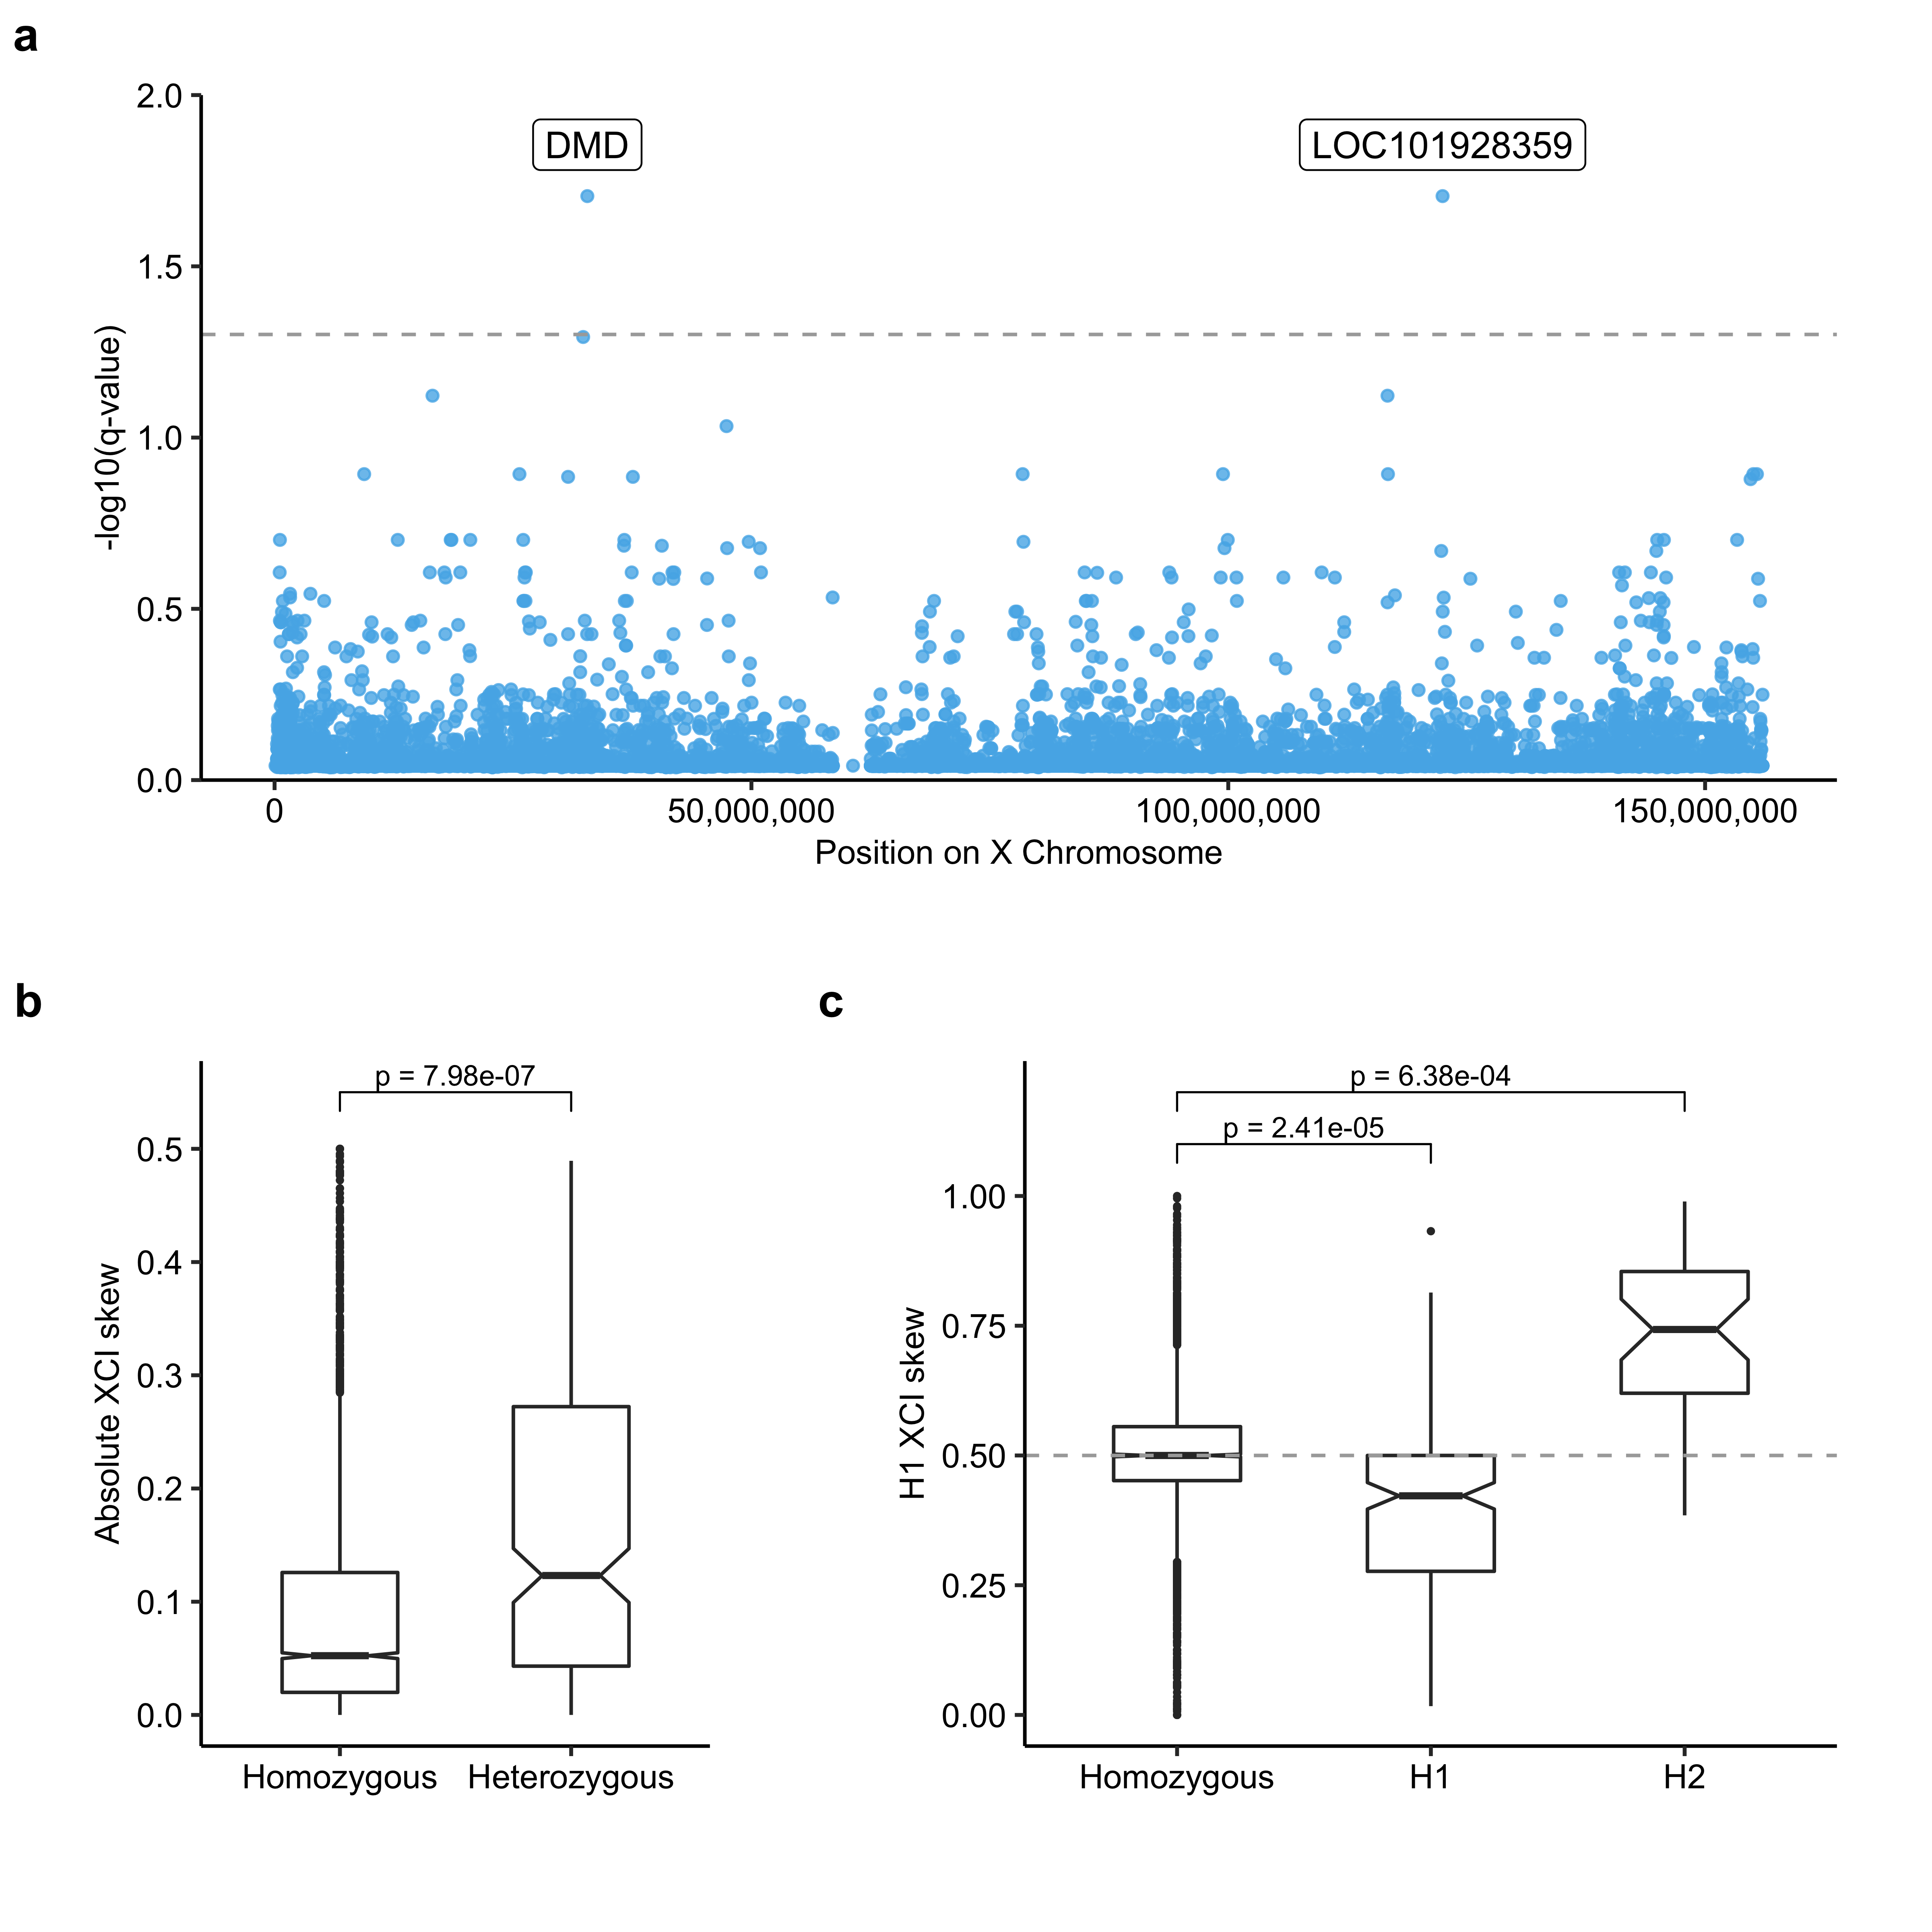
\includegraphics[width=0.75\textwidth]{chapter4/Figures/Figure_3.png}
    \caption{
        Associating specific variation on the X chromosome with inactivation skew. 
        \textbf{a}, Manhattan plot of -log10(q-values) generated from a linear mixed model associating absolute XCI skew with heterozygous status, accounting for age as well as individual and tissue groupings of samples. A one-sided test was performed under the hypothesis that heterozygous status increases absolute skew. Dotted horizontal line indicates local false discovery rate of 0.05. 
        \textbf{b}, Boxplot of absolute XCI skew in samples that are homozygous  (n = 4,232) or heterozygous (n = 230) for the DMD variant (rs141680486). Indicated p-value is from the model described above.
        \textbf{c}, Boxplot of skewing toward haplotype 1 (H1), where the grouping on the x-axis describes individuals without the DMD variant (Homozygous, n = 4,232), with the variant on haplotype 1 (H1, n = 190), and with the variant on haplotype 2 (H2, n = 40). Indicated p-values are from the model described above but with a two-sided test, since we do not assume the direction of skewing associated with a specific variant.}
    \label{fig:fig4.3}
\end{figure}
\begin{figure}[ht!]
    \centering
    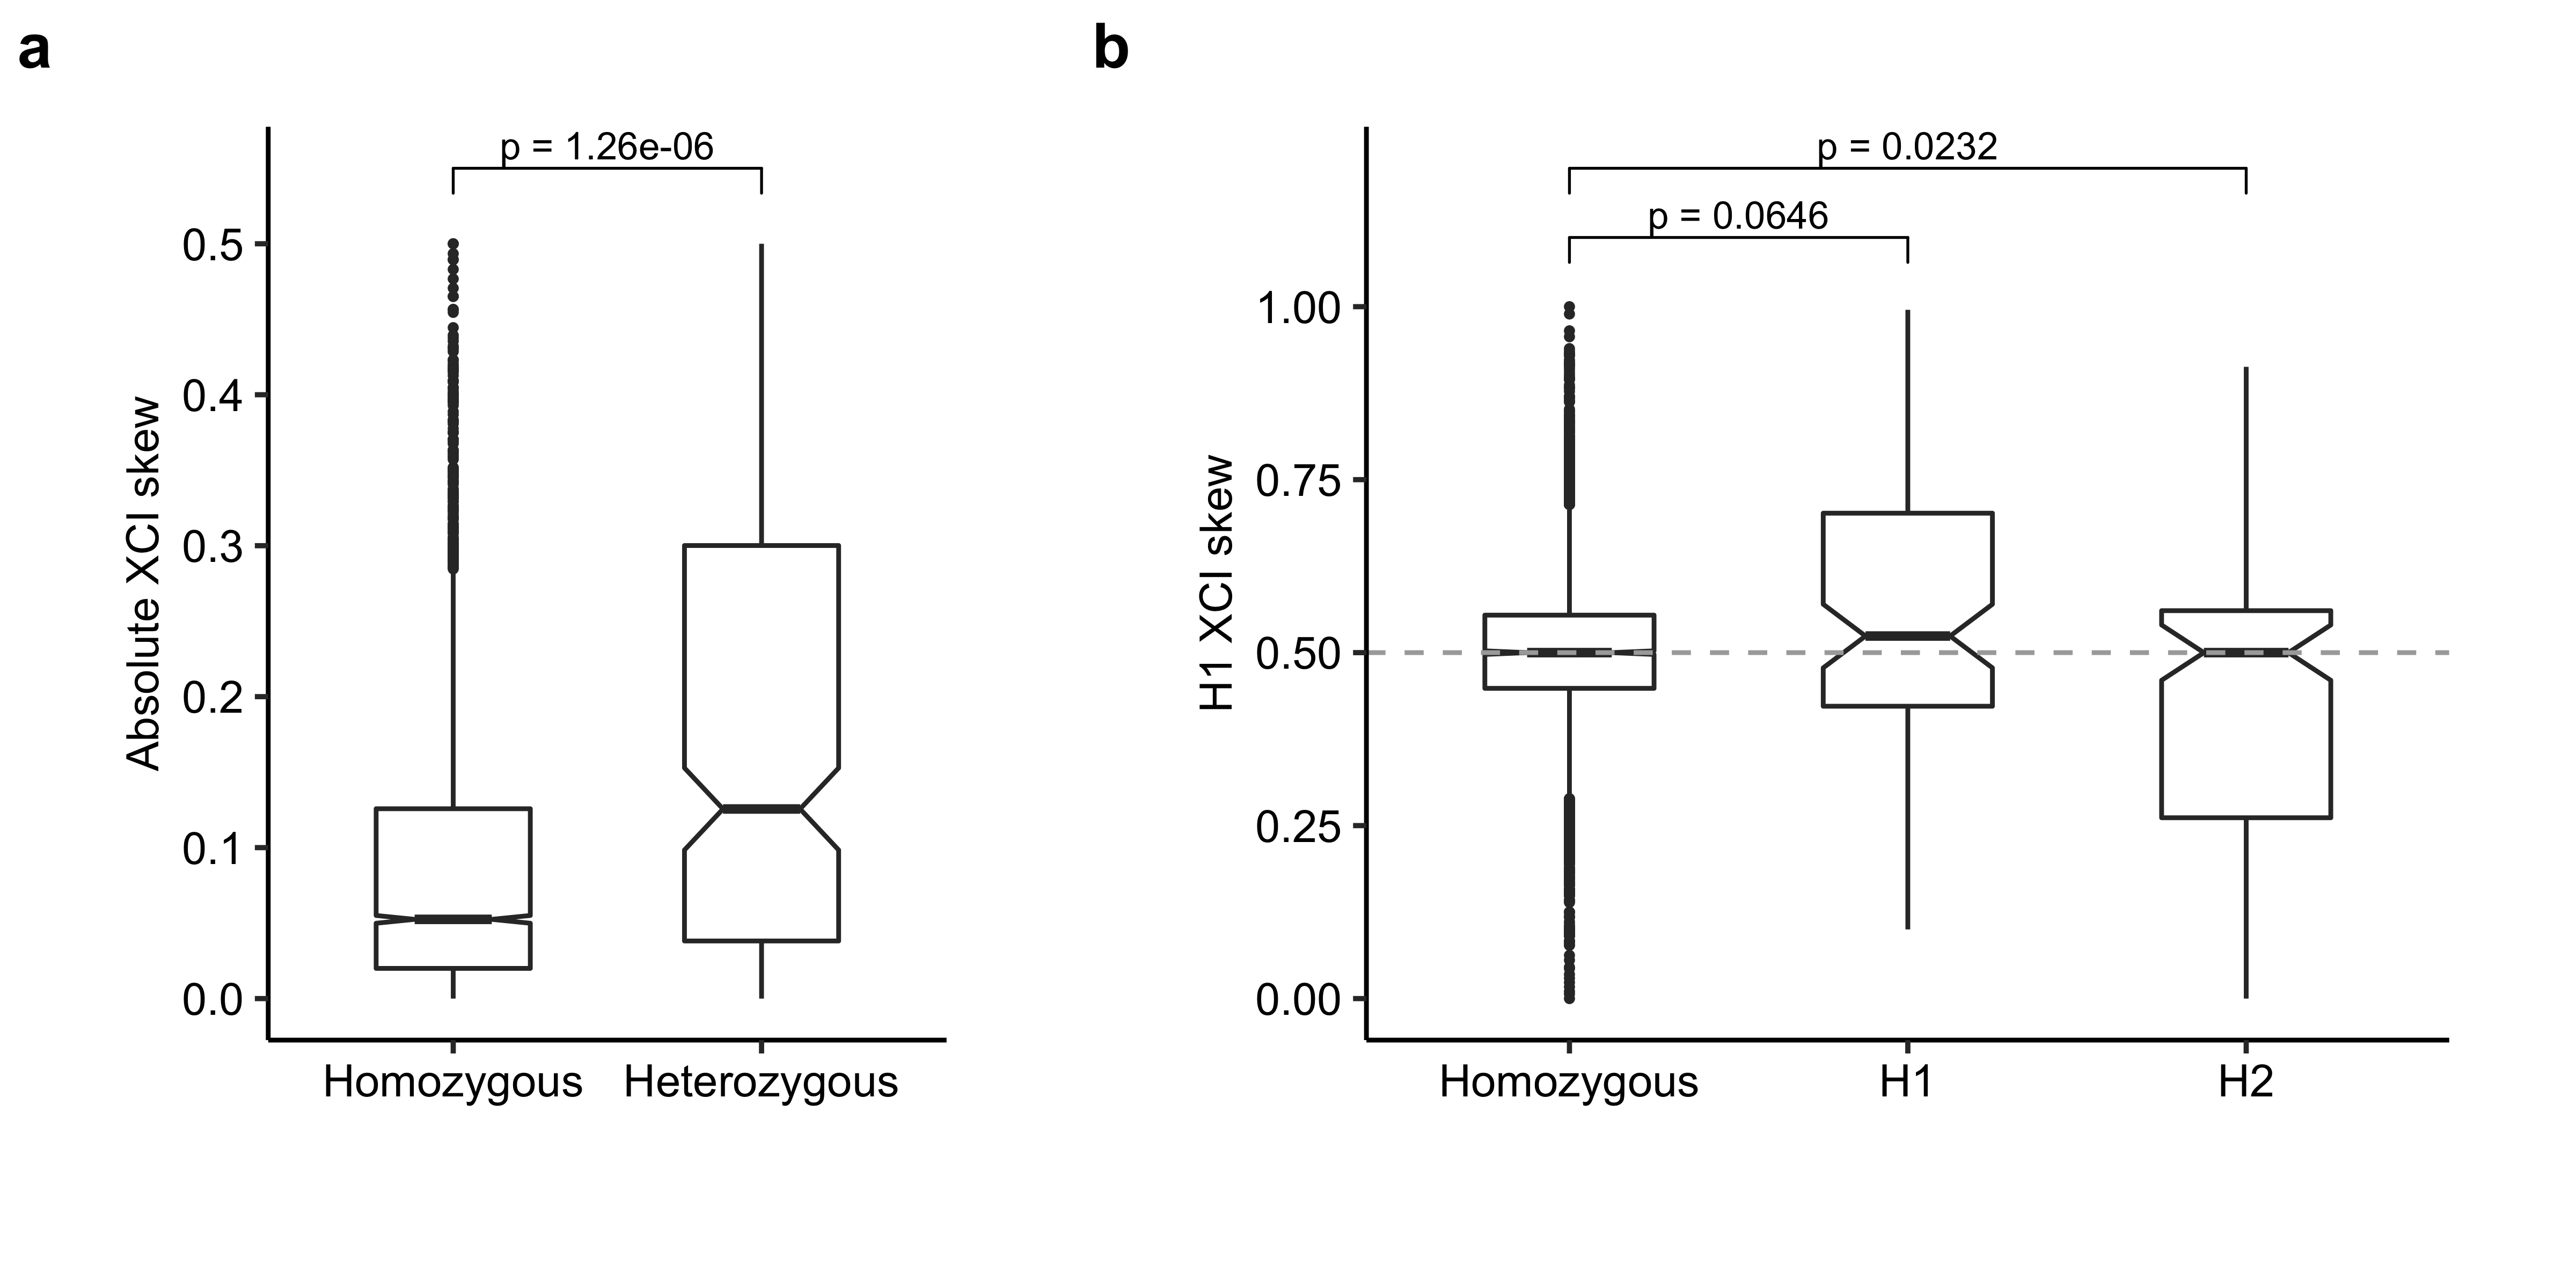
\includegraphics[width=0.9\textwidth]{chapter4/Figures/Supplementary_Figure_4.png}
    \caption{
        Association of LOC101928359 variant (rs73227260) variants with XCI skew. Indicated p-values are from a linear mixed model accounting for individual and tissue of origin.
        \textbf{a}, Boxplot of absolute XCI skew in homozygous samples (n = 4,230) and heterozygous samples (n = 232). Indicated p-value is from a one-sided t-test.
        \textbf{b}, Boxplot of skewing toward haplotype 1 (H1), where the grouping on the x-axis describes individuals without the LOC variant (Homozygous, n = 4,230), with the variant on haplotype 1 (H1, n = 92), and with the variant on haplotype 2 (H2, n = 140). Indicated p-values are from two-sided t-test.  
    }
    \label{fig:supp_fig4.4}
\end{figure}
\begin{table}[ht]
\scriptsize
\caption{Top 10 variants associated with absolute skewing in XCI}
\centering
\begin{tabular}{lllllll}
  \hline
Locus & SNP & Position & Alleles & AF & $\beta$ (s.e.) & $P_{\text{one-sided}}$ \\ 
  \hline
  DMD & rs141680486 & 32794582 & C/G & 0.0179 & 0.0203 (0.0041) & 7.978e-07 \\ 
  LOC101928359 & rs73227260 & 122471389 & C/T & 0.0203 & 0.0199 (0.0041) & 1.265e-06 \\ 
  DMD & rs144615018 & 32355895 & C/G & 0.0328 & 0.0175 (0.0039) & 4.891e-06 \\ 
  None & rs140456300 & 116700067 & A/T & 0.0316 & 0.0157 (0.0036) & 9.868e-06 \\ 
  None & rs113265091 & 16560720 & T/C & 0.0185 & 0.0177 (0.0041) & 1.21e-05 \\ 
  ZNF157 & rs140428205 & 47388509 & G/A & 0.0215 & 0.0174 (0.0041) & 1.782e-05 \\ 
  None & rs60102760 & 9394922 & T/G & 0.0263 & 0.0168 (0.0041) & 2.917e-05 \\ 
  FUNDC2 & rs782070621 & 155057031 & T/G & 0.0369 & 0.0169 (0.0042) & 3.742e-05 \\ 
  None & rs139564137 & 155434572 & C/T & 0.0358 & 0.0169 (0.0042) & 3.742e-05 \\ 
  None & rs6623805 & 78439230 & A/T & 0.9475 & 0.0159 (0.004) & 4.263e-05 \\ 
   \hline
\end{tabular}
\label{table:table4.3}
\end{table}

\section{Discussion}

These analyses support the hypothesis that differences in genetic variation on the maternal and paternal X chromosomes influences skewed inactivation through selection \cite{Brown1999-dc,Migeon1998-gc}. Specifically, these results demonstrate a significant association between higher CADD scores of a haplotype and skewing away from this haplotype. Furthermore, we showed that higher polygenic scores related to proliferation, specifically red blood cell and basophil counts, tend to be associated with skewing towards the haplotype. These results imply that skewing in X inactivation may arise from higher proliferation or reduced deleteriousness of cells with one haplotype activated compared to the other subpopulation. We also identified common variation within specific loci on the X chromosome, such as the dystrophin gene, associated with XCI skew that may also contribute to these differences in proliferation or deleteriousness.

Several confounding factors could influence the results of this study. First, haplotype estimation by phasing algorithms may be inaccurate. Phasing errors would reduce the power of these analyses, since genetic scores may include variants from both haplotypes. In our analyses, we observed phase switches in EBV-transformed lymphocyte samples with extreme XCI skewing that suggests some phasing errors had occurred. Second, mapping biases may cause artificially higher observed expression of reference alleles compared to alternate alleles. This issue is addressed by the WASP filtering \cite{Van_de_Geijn2015-oy} used in the alignment of RNA-seq reads. Third, differences in eQTL effects across haplotypes may lead to skewed expression in RNA-seq experiments that may be incorrectly attributed to skewed XCI. We consider this source of confounding by taking the median of expression skew measured across heterozygous sites in 117 fully inactivated genes and by testing whether our features of interest are significant in the non-acrocentric autosomes or as eQTLs in the male samples. These issues could be circumvented with sufficiently large single-cell RNA-seq datasets. Haplotype phasing, as well as inactivation status, could be estimated within each cell individually and XCI skew could be calculated by simply counting cells. Furthermore, these data would allow cell-type-specific analysis of the relationship between genetics and skewed XCI.  

The influence of genetics on XCI skewing across the general female population highlights interesting mechanisms that should be further explored. For example, the effect of a specific variant on a complex phenotype may be dampened or amplified depending on the haplotype that carries it in females. For example, if an individual homozygous for a disease-related variant carries it on a haplotype with reduced proliferation, its effect may be dampened since a majority of cells will be expressing the wild-type variant. Epistatic effects and reduced penetrance due to allele-specific expression has been previously reported in the context of allele-specific gene regulation \cite{Castel2018-wo,Lappalainen2011-mu}. Here, these effects would arise from skewed X inactivation across a tissue rather than skewed expression within individual cells. This effect on penetrance has been described in the context of X-linked disorders, where skewed inactivation blurs the distinction of dominant and recessive traits across males and females \cite{Dobyns2004-ac}. The results shown here imply that selective pressures on genetic differences across the female population can influence skewing and consequently influence the penetrance of variation across the X chromosome.
%\input {chapter5}
%\input {chapter6}
%\input {chapter7}
%\input {chapter8}

\chapter{Introduction}
\section{Scope of Research}
Advances in sequencing technologies have paved the way for the generation of large-scale genomic datasets capturing genetic and transcriptomic variation across diverse sets of individuals \cite{Bycroft2018, GTEx_Consortium2020-xx}. These data allow researchers to elucidate the relationship between genetics, gene expression, and complex phenotypes \cite{Gusev2016}. Genome-wide association studies have identified a vast number of genetic loci associated with different traits \cite{gwas} and the identification of expression quantitative trait loci (eQTLs) bridges the gap between genotype and phenotype by elucidating the effects of genetic variation on gene expression \cite{Nica2013}. These associations serve as stepping stones for better understanding of human health and potential therapeutic targets \cite{Motsinger-Reif2013, walker2001pharmaceutical}. However, studies involving tissue-level gene expression are hindered by confounding factors that can both decrease power to detect associations and cause spurious results.

Many tissues in the human body consist of several cell types. For example, brain tissue often contains an assortment of neuronal and glial cell populations, each with distinct functions and gene expression profiles. RNA sequencing (RNA-seq) is often performed on whole tissues and analyses of these data can be confounded by cell-type heterogeneity across samples \cite{farahbod2020untangling}. Differences in cell type composition can be misinterpreted as differences in gene expression levels when measuring RNA across tissues. Furthermore, these mixtures can obscure cell-type-specific gene regulation that may be of interest \cite{Westra2015-vq, Shen-Orr2010-tg}. Single-cell approaches, such as single-cell RNA-seq (scRNA-seq) and single-nucleus RNA-seq (snRNA-seq), avoid these issues and provide insight into the gene expression of individual cells. However, these experiments remain costly, noisy, and difficult to scale compared to bulk RNA-seq \cite{lahnemann2020eleven}. Given the continuing utility of tissue-level RNA-seq datasets, it is important to accurately model variability in cell type proportions in these samples.

Regulation of gene expression also varies significantly across tissues \cite{GTEx_Consortium2020-xx}. Moreover, several tissues can have distinct roles in biological systems underlying a complex phenotype. For example, analyses of Type II diabetes have observed transcriptomic changes in blood \cite{Christodoulou2019}, adipose \cite{Miao2020}, and brain \cite{Zhou2019}. Therefore, it is imperative to measure gene expression across many tissues to fully understand gene regulation and its role in traits of interest. Analyzing gene expression across tissues, especially with growing sample sizes, requires approaches that can model this heterogeneity both accurately and efficiently.

Finally, the relationship between gene expression and genetic variation is highly complex \cite{robert2018exploring} and remains to be fully understood. Many eQTLs have been identified and are thought to influence gene expression through interactions with regulatory regions of the genome, such as enhancers and promoters \cite{Garieri2017}. Alternative mechanisms of genetic influences on gene regulation have been hypothesized, specifically in the context of selective pressures causing non-random X chromosome inactivation \cite{Migeon1998-gc}. To better understand human biology, it is important to validate these hypotheses and identify the extent of their influence on regulation of gene expression. 

\section{Contributions and Overview}
In this dissertation, we introduce computational and statistical methods to accurately model tissue-level expression data with heterogeneity in cell composition and tissue identity. Furthermore, we present analyses of expression data that yields further insight into non-random X chromosome inactivation as an additional mechanism for gene regulation with several interesting implications in the context of X-linked phenotypes.

There is large interest in estimating cell type proportions from tissue-level RNA-seq data. These estimates allow researchers to account for this potential confounding factor in analyses of gene expression data, such as eQTL and differential expression studies. Furthermore, cell type proportions can be used with additional methods to identify cell-type-specific associations from tissue-level data \cite{Shen-Orr2010-tg}. In Chapter 2, we describe Bisque, an approach for accurately estimating cell type proportions from bulk RNA-seq data. This method utilizes available single-cell data as a reference for cell-type-specific expression while accounting for technological biases between bulk and single-cell RNA-seq.

In Chapter 3, we present an efficient linear mixed model (LMM) for the analysis of massive datasets measuring multiple contexts across a set of individuals. This method, mcLMM, models all contexts jointly in a meta-analytic framework to improve power to detect associations. It can be applied to large expression datasets with measurements across several tissues, such as the GTEx dataset \cite{GTEx_Consortium2020-xx}, to efficiently identify genetic variants that influence gene regulation in specific tissues or across several tissues. We further demonstrate the utility of this method by performing a multi-trait genome-wide association study across hundreds of thousands of individuals in the UK Biobank \cite{Bycroft2018} using minimal computational resources.

In Chapter 4, we analyze the GTEx dataset \cite{GTEx_Consortium2020-xx} to support the hypothesis of selective pressures influencing non-random X chromosome inactivation \cite{Migeon1998-gc} and quantify the extent of this effect in the female population. We estimate skewing in X inactivation from bulk RNA-seq data measured across non-diseased tissue samples and identify several genetic factors that are significantly associated with preferential inactivation of a haplotype, such as variation associated with increased deleteriousness and decreased proliferation. Furthermore, we identify common genetic variants in specific loci that contribute to skewed X chromosome inactivation. We highlight the implications of non-random skew in X chromosome inactivation, such as decreased penetrance or dampened effects of genetic variation on preferentially inactivated haplotypes.

\setlength{\arrayrulewidth}{1.1pt}
\newcolumntype{L}{>{\raggedright\arraybackslash}X}
\bgroup
\def\arraystretch{1.5}

\chapter{Accurate estimation of cell composition in bulk expression through robust integration of single-cell information}

\section{Background}

Bulk RNA-seq experiments typically measure total gene expression from heterogeneous tissues, such as tumor and blood samples~\cite{Tomczak2015-kt,GTEx_Consortium2015-vl}. Variability in cell type composition can significantly confound analyses of these data, such as in identification of expression quantitative trait loci (eQTLs) or differentially expressed genes~\cite{Bruning2016-vb}. Cell type heterogeneity may also be of interest in profiling changes in tissue composition associated with disease, such as cancer~\cite{Fridman2012-bi} or diabetes~\cite{Rahier1983-gh}. In addition, measures of cell composition can be leveraged to identify cell-specific eQTLs~\cite{Shen-Orr2010-tg,Westra2015-vq} or differential expression~\cite{Shen-Orr2010-tg} from bulk data. 

Traditional methods for determining cell type composition, such as immunohistochemistry or flow cytometry, rely on a limited set of molecular markers and lack in scalability relative to the current rate of data generation~\cite{Hu2016-he}. Single-cell technologies provide a high-resolution view into cellular heterogeneity and cell type-specific expression~\cite{Zheng2017-pq,Tasic2018-ue,Macosko2015-yn}. However, these experiments remain costly and noisy compared to bulk RNA-seq~\cite{Wang2018-oj}. Collection of bulk expression data remains an attractive approach for identifying population-level associations, such as differential expression regardless of cell type specificity. Moreover, many bulk RNA-seq studies that have been performed in recent years resulted in a large body of data that is available in public databases such as dbGAP and GEO. Given the wide availability of these bulk data, the estimation of cell type proportions, often termed decomposition, can be used to extract large-scale cell type specific information.

There exist a number of methods for decomposing bulk expression, many of which are regression-based and leverage cell type-specific expression data as a reference profile~\cite{Mohammadi2017-rw}. CIBERSORT~\cite{Newman2015-iw} is a SVM-regression based approach, originally designed for microarray data, that utilizes a reference generated from purified cell populations. A major limitation of this approach is the reliance on sorting cells to estimate a reference gene expression panel. BSEQ-sc~\cite{Baron2016-hb} instead generates a reference profile from single-cell expression data that is used in the CIBERSORT model. MuSiC~\cite{Wang2019-lc} also leverages single-cell expression as a reference, instead using a weighted non-negative least squares regression (NNLS) model for decomposition, with improved performance over BSEQ-sc in several datasets.

The distinct nature of the technologies used to generate bulk and single-cell sequencing data may present an issue for decomposition models that assume a direct proportional relationship between the single-cell-based reference and observed bulk mixture. For example, the capture of mRNA and chemistry of library preparation can differ significantly between bulk tissue and single-cell RNA-seq methods, as well as between different single-cell technologies~\cite{Ziegenhain2017-ss,La_Manno2018-tx}. Moreover, some technologies may be measuring different parts of the transcriptome, such as nuclear pre-mRNA in single-nucleus RNA-seq (snRNA-seq) experiments as opposed to cellular and extra-cellular mRNA observed in traditional bulk RNA-seq experiments. As we show later, these differences may introduce gene-specific biases that break down the correlation between cell type-specific and bulk tissue measurements. Thus, while single-cell RNA-seq technologies have provided unprecedented resolution in identifying expression profiles of cell types in heterogeneous tissues, these profiles generally may not follow the direct proportionality assumptions of regression-based methods, as we demonstrate here.

We present Bisque, a highly efficient tool to measure cellular heterogeneity in bulk expression through robust integration of single-cell information, accounting for biases introduced in the single-cell sequencing protocols. The goal of Bisque is to integrate the different chemistries/technologies of single-cell and bulk tissue RNA-seq to estimate cell type proportions from tissue-level gene expression measurements across a larger set of samples. Our reference-based model decomposes bulk samples using a single-cell-based reference profile and, while not required, can leverage single-cell and bulk measurements for the same samples for further improved decomposition accuracy. This approach employs gene-specific transformations of bulk expression to account for biases  in sequencing technologies as described above. When a reference profile is not available, we propose BisqueMarker, a semi-supervised model that extracts trends in cellular composition from normalized bulk expression samples using only cell-specific marker genes that could be obtained using single cell data. We demonstrate using simulated and real datasets from brain and adipose tissue that our method is significantly more accurate than existing methods. Furthermore, it is extremely efficient, requiring seconds in cases where other methods require hours; thus, it is scalable to large genomic datasets that are now becoming available.

\section{Methods}

\subsection{Processing bulk expression data}

Paired-end reads were aligned with STAR v2.5.1 using default options.  Gene counts were quantified using featureCounts v1.6.3. For featureCounts, fragments were counted at the gene-name level. Alignment and gene counts were generated against the GRCh38.p12 genome assembly. STAR v2.5.1 and GRCh38.p12 were included with CellRanger 3.0.2, which was used to process the single-nucleus data.

\subsection{Processing single-nucleus expression data}

Reads from single nuclei sequenced on the 10x Genomics Chromium platform were aligned and quantified using the CellRanger 3.0.2 count function against the GRCh38.p12 genome assembly. To account for reads aligning to both exonic and intronic regions, each gene transcript in this reference assembly was relabeled as an exon since CellRanger counts exonic reads only. We perform this additional step since snRNA-seq captures both mature mRNA and pre-mRNA, the latter of which includes intronic regions. 

After aggregating each single-nucleus sample with the CellRanger aggr function, the full dataset was processed using Seurat v3.0.0~\cite{Butler2018-mj}. The data were initially filtered for genes expressed in at least 3 cells and filtered for cells with reads quantified for between 200 and 2,500 genes. We further filtered for cells that had a percentage of counts coming from mitochondrial genes less than or equal to 5 percent. The data were normalized, scaled, and corrected for mitochondrial read percentages with sctransform v0.2.0~\cite{Hafemeister_undated-xh} using default options.

To identify clusters, Seurat employs a shared nearest neighbor approach. We identified clusters using the top 10 principal components of the processed expression data with resolution set at 0.2. The resolution parameter controls the number of clusters that will be identified, and suggested values vary depending on the size and quality of the dataset. We chose a value that produced 6 clusters in the adipose dataset and 13 clusters in the DLPFC dataset and visualized the clustering results with UMAP~\cite{McInnes2018-lp}. 

Marker genes were identified by determining the average log-fold change of expression of each cluster compared to the rest of the cells. We identified marker genes as those with an average log-fold change above 0.25. The significance of the differential expression of these genes was determined using a Wilcoxon rank sum test. Only genes that were detected in at least 25 percent of cells were considered. Clusters with many mitochondrial genes as markers (nine genes detected in both datasets) were removed from both datasets. In addition, a cluster with only three marker genes was removed from the DLPFC datasets. Finally, we remove mitochondrial genes from the list of marker genes for decomposition as we assume reads aligning to the mitochondrial genome originate from extra-nuclear RNA in the snRNA-seq dataset (targeting nuclear RNA). 

Clusters were labeled by considering cell types associated with the identified marker genes. Marker genes were downloaded from PanglaoDB~\cite{Franzen2019-nb} and filtered for entries validated in human cells. For each gene, we count the possible cell type labels. Each cluster was labeled as the most frequent cell type across all of its marker genes, with each label associated with a gene weighted by the average log-fold change. If multiple clusters share a cell type label, we consider each cluster a subtype of this label. 

Exon-aligned reads were processed in the same exact procedure but snRNA-seq data was aligned to just exonic regions. Cluster names were manually changed for both datasets when aligned to exons to match the clusters from intronic reads as well. Specifically, for clusters identified in the exonic data not found in the full data, we relabeled as the label with the highest score found in the full data. These relabeled clusters were similar in proportion to the corresponding cluster in the full dataset.

\subsection{Learning a single-cell based reference and bulk transformation for reference-based decomposition}

We assume that only a subset of genes are relevant for estimating cell type composition. For the adipose and DLPFC datasets, we selected the marker genes identified by Seurat as described previously. Moreover, we filter out genes with zero variance in the single-cell data, unexpressed genes in the bulk expression, and mitochondrial genes. We convert the remaining gene counts to counts-per-million to account for variable sequencing depth. For $m$ genes and $k$ cell types, a reference profile $Z \in \mathbb{R}^{m \times k}$ is generated by averaging relative abundances within each cell type across the entire single-cell dataset.

Though there is a strong positive correlation between bulk and single-cell based pseudo-bulk (summed single-cell counts) expression data, we observe that the relationship is not one-to-one and varies between genes. This behavior indicates that the distribution of observed bulk expression may significantly differ from the distribution of the single-cell profile weighted by cell proportions. We propose transforming the bulk data to maximize the global linear relationship across all genes for improved decomposition. Our goal is to recover a one-to-one relationship between the transformed bulk and expected convolutions of the reference profile based on single-cell based estimates of cell proportions. This transformed bulk expression better satisfies the assumptions of regression-based approaches under sum-to-one constraints. 

Cell type proportions $p \in \mathbb{R}^{k \times n'}$ are determined by counting the cells with each label in the single-cell data for  individuals. Given these proportions and the reference profile $Z$, we calculate the pseudo-bulk for the single-cell samples as 
\begin{equation}
    Y=Zp
\end{equation}
where $Y \in \mathbb{R}^{m \times n'}$. For each gene $j$, our goal is to transform the observed bulk expression across all $n$ bulk samples $X_j \in \mathbb{R}^n$ to match the mean and variance of $Y_j \in \mathbb{R}^{n'}$; hence, the transformation of $X_j$ will be a linear transformation. 

If individuals with both single-cell and bulk expression are available, we fit a linear regression model to learn this transformation. Let $X'_j$ denote the expression values for these $n'$ overlapping individuals. We fit the following model (with an intercept) and apply the model to the remaining bulk samples as our transformation:
\begin{equation}
	Y_j = \beta_jX'_j + \epsilon_j
\end{equation}
If there are no single-cell samples that have bulk expression available, we assume that the observed mean of $Y_j$ is the true mean of our goal distribution for the transformed $X_j$. We further assume that the sample variance observed in $Y_j$ is larger than the true variance of the goal distribution, since the number of single-cell samples is typically small. We use a shrinkage estimator of the sample variance of $Y_j$ that minimizes the mean squared error and results in a smaller variance than the unbiased estimator:
\begin{equation}
	\hat{\sigma}^2_j = \frac{1}{n' + 1} \sum_{i=1}^{n'}(Y_{i,j} - \bar{Y}_j)^2
\end{equation}
We transform the remaining bulk as follows:
\begin{equation}
	X_{j,transformed} = \frac{X_j - \bar{X}_j}{\sigma_{X_j}} \hat{\sigma}_j + \bar{Y}_j
\end{equation}
where a bar indicates the mean value of the observed data and $\sigma_{X_j}$ is the unbiased sample standard deviation of  $X_j$.

To estimate cell type proportions, we apply non-negative least squares regression with an additional sum-to-one constraint to the transformed bulk data. For individual $i$, we minimize the following with respect to the cell proportion estimate $p_i$:
\begin{equation}
    \left\lVert Zp_i - X_{i,transformed} \right\rVert_2 \text{ s.t. } p_i \geq 0,\text{ } \sum p_i = 1 
\end{equation}

\subsection{Simulating bulk expression based on single-nucleus counts}

We simulate the base bulk expression as the sum of all counts across cells/nuclei sequenced from an individual. To introduce gene-specific variation between the bulk and single-cell data, we sample a coefficient $\beta_j$ and an intercept $\alpha_j$ from a half-normal (HN) distributions:
\begin{equation}
    \beta_j \sim HN(1,\sigma)
\end{equation}
\begin{equation}
    \alpha_j \sim HN(0,\sigma)
\end{equation}
where the variance of the HN distribution is $\sigma^2(1-\frac{2}{\pi})$. At $\sigma = 0$, the base simulated bulk expression remains unchanged. We used a HN distribution to ensure coefficients and intercepts are positive. While our method can handle negative coefficients, this simulation model assumes expression levels have a positive correlation across technologies. We performed 10 replicates of this data-generating process at each $\sigma$ in 0, 5, 10, 20. Decomposition performance on these data were measured in terms of global R and RMSD and plotted with 95\% confidence intervals based on bootstrapping. 

\subsection{Determining significance of cell proportion associations with measured phenotypes}

Reported associations were measured in terms of Spearman correlation. To determine the statistical significance of these associations while accounting for possible confounding factors, we applied two approaches. For the adipose dataset, which consisted entirely of twin pairs, we applied a linear mixed-effects model (R nlme package) with random effects accounting for family. For the DLPFC dataset, we assumed individuals were unrelated and fit a simple linear model (R base package). In each model, we include cell type proportion, age, age-squared, and sex as covariates. We introduced an additional covariate for diabetes status when regressing the Matsuda index due to a known significant association between these two variables. We test whether the cell proportion effect estimates deviate significantly from 0 using a t-test. Each R method implements the described model fitting and significance testing.

\subsection{Estimating relative cellular heterogeneity with a semi-supervised weighted PCA model}

In order to estimate cell type proportions across individuals without the use of a cell-type-specific gene expression panel as reference, we use a weighted PCA approach. BisqueMarker requires a set of marker genes for each cell type as well as the specificity of each marker determined by the fold change from a differential expression analysis. Typical single-cell RNA-seq workflows calculate marker genes and provide both p-values and fold changes, as in Seurat~\cite{Butler2018-mj}. For each cell type, we take statistically significant marker genes (FDR $<$ 0.05) ranked by p-value. A weighted PCA is calculated on the expression matrix using a subset of the marker genes by first scaling the expression matrix and multiplying each gene column by its weight (the log fold-change) $XW$, where $X$ is the sample by gene expression matrix and $W$ is a diagonal matrix with entries equal to log fold-change of the corresponding gene. The bulk expression $X$ should be corrected for global covariates so that the proportion estimates do not reflect this global variation. The first PC calculated from $XW$ is used as the estimate of the cell type proportion. This allows cell type-specific genes to be prioritized over more broadly expressed genes. Alternatively, if weights are not available, PCA can be run on the matrix $X$ and the first PC can be used.

In order to select marker genes, we iteratively run the above PCA procedure on a specified range of markers (from 25 to 200) and calculate the ratio of the first eigenvalue to the second. We then select the number of marker genes to use that maximizes this ratio. This procedure is similar to other methods which select the number of markers to use by maximizing the condition number of the reference matrix~\cite{Mohammadi2017-rw}. 

\section{Results}
\subsection{Overview of Bisque}

A graphical overview of Bisque is presented in Figure \ref{fig:fig2.1}. Our reference-based decomposition model requires bulk RNA-seq counts data and a reference dataset with read counts from single-cell RNA-seq. In addition, the single-cell data should be labeled with cell types to be quantified. A reference profile is generated by averaging read count abundances within each cell type in the single-cell data. Given the reference profile and cell proportions observed in the single-cell data, our method learns gene-specific transformations of the bulk data to account for technical biases between the sequencing technologies. Bisque can then estimate cell proportions from the bulk RNA-seq data using the reference and the transformed bulk expression data using non-negative least-squares (NNLS) regression. 

%% Figure 1
\begin{figure}
    \centering
    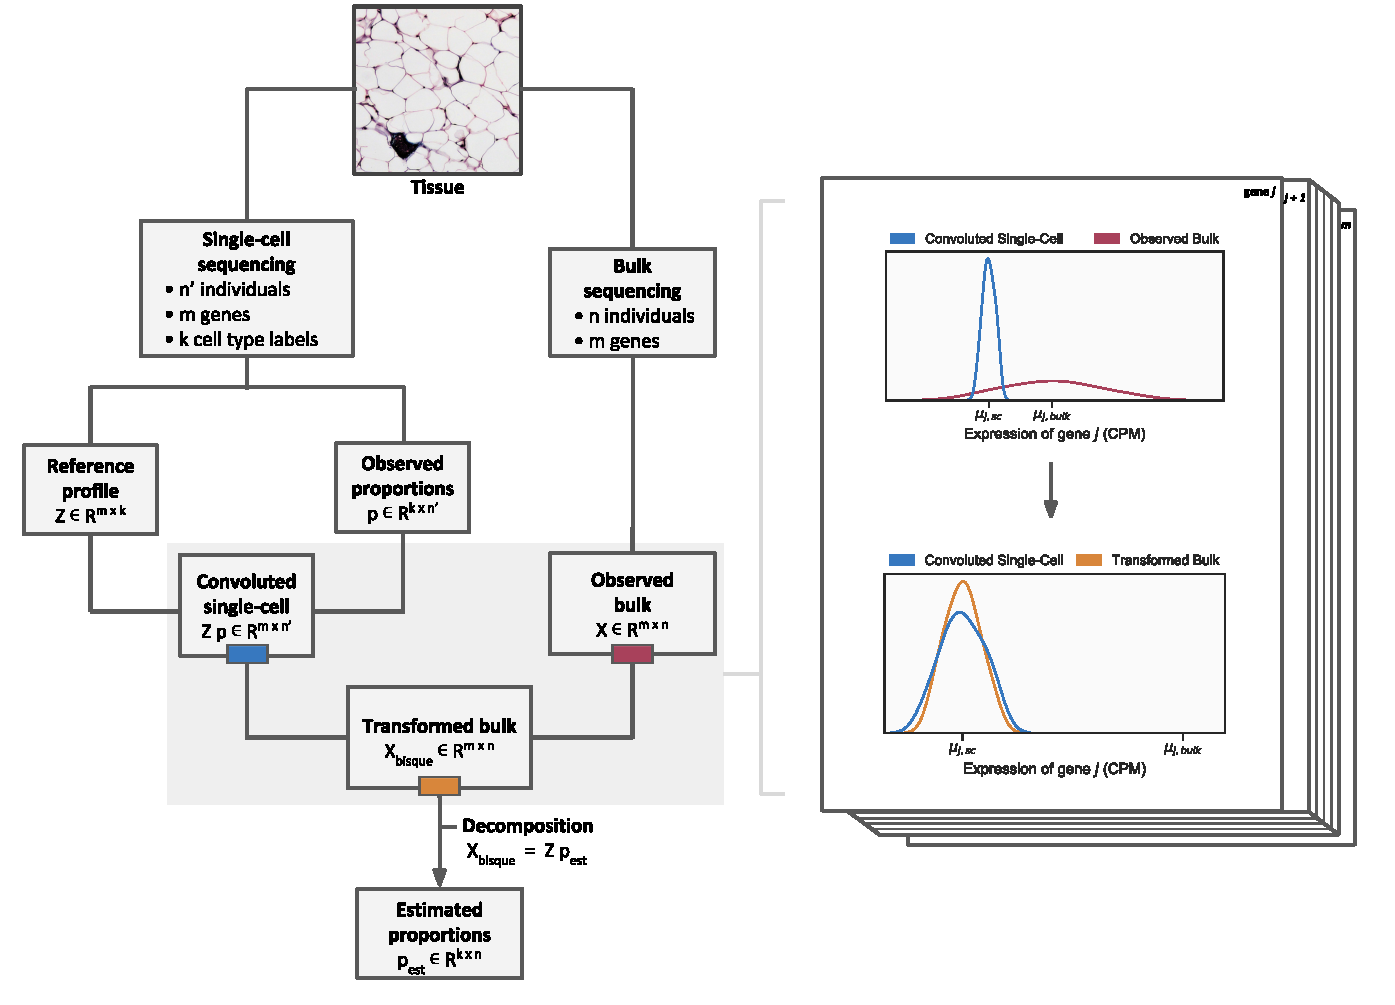
\includegraphics[width=\textwidth]{chapter2/figures/fig1.pdf}
    \caption{
            Graphical overview of the Bisque decomposition method. We integrate single-cell and bulk expression by learning gene-specific bulk transformations (pictured on right) that align the two datasets for accurate decomposition.
            }
    \label{fig:fig2.1}
\end{figure}

\subsection{Evaluation of decomposition performance in adipose tissue}
We applied our method to 106 bulk RNA-seq subcutaneous adipose tissue samples collected from both lean and obese individuals, where 6 samples have both bulk RNA-seq and snRNA-seq data available (Table \ref{table:table2.1}). Adipose tissue consists of several cell types, including adipocytes which are expected to be the most abundant population. Adipose tissue also contains structural cell types (i.e. fibroblasts and endothelial cells) and immune cells (i.e. macrophages and T cells)~\cite{Esteve_Rafols2014-ia}. These 5 cell type populations were identified from the snRNA-seq data (Figure \ref{fig:supfig2.1}a).

\begin{table}
    \scriptsize
    \centering
    \begin{tabularx}{\textwidth}{|L|L|L|L|L|p{1cm}|L|L|}
    \hline
    \rowcolor{mygray}
    \textbf{Tissue} & \textbf{Number of Samples} & \textbf{Bulk RNA-seq platform} & \textbf{snRNA-seq platform} & \textbf{snRNA-seq samples} & \textbf{Total nuclei} & \textbf{Average nuclei per individual} & \textbf{Number of cell types}  \\ \hline
    Subcutaneous adipose & 106 & Illumina NovaSeq & 10x Genomics Chromium & 6 & 10,947 & 1,824 & 5  \\ \hline
    Dorsolateral prefrontal cortex & 636 & Illumina HiSeq & 10x Genomics Chromium & 8 & 68,028 & 8,503 & 11  \\
    \hline
    \end{tabularx}
    \captionsetup{justification=raggedright,singlelinecheck=false}
    \caption{
        Summary of snRNA-seq and bulk expression datasets used for benchmarking Bisque and existing methods. 
        }
    \label{table:table2.1}
\end{table}

\begin{figure}
\centering
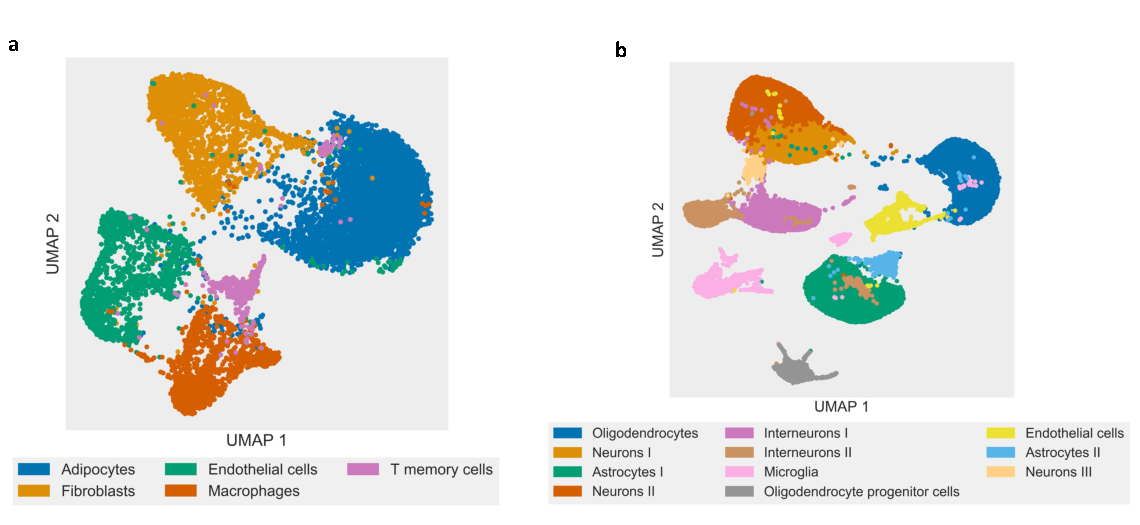
\includegraphics[width=\textwidth]{chapter2/figures/supfig1-2.pdf} 
\caption{
         Cell types quantified in snRNA-seq experiments.
         (\textbf{a}) UMAP projection of adipose snRNA-seq data with 5 identified cell type clusters labeled. (\textbf{b}) UMAP projection of cortex snRNA-seq data with 11 identified clusters.
        }
\label{fig:supfig2.1}
\end{figure}

We observed significant biases between the snRNA-seq and bulk RNA-seq data in samples that had both data available. We found that the linear relationship between the pseudo-bulk (summed snRNA-seq reads across cells) and the true bulk expression varied significantly by each gene (Figure \ref{fig:fig2.2}a). Specifically, we observed best fit lines relating these expression levels between technologies with a mean slope of roughly 0.30 and a variance in slope of 5.67. In our model, a slope of 1 would indicate no bias between technologies. We further investigated whether gene expression differences between the bulk and snRNA-seq were the same across individuals and experiments. Comparing log-ratios of RNA-seq to snRNA-seq expression levels, we found that the majority of gene biases were preserved across individuals, tissues, and experiments (R=0.75 across experiments) (Figure \ref{fig:supfig2.3}), providing evidence that technological differences drive consistent gene expression differences across bulk and snRNA-seq methods. 

\begin{figure}
\centering
\begin{multicols}{2}
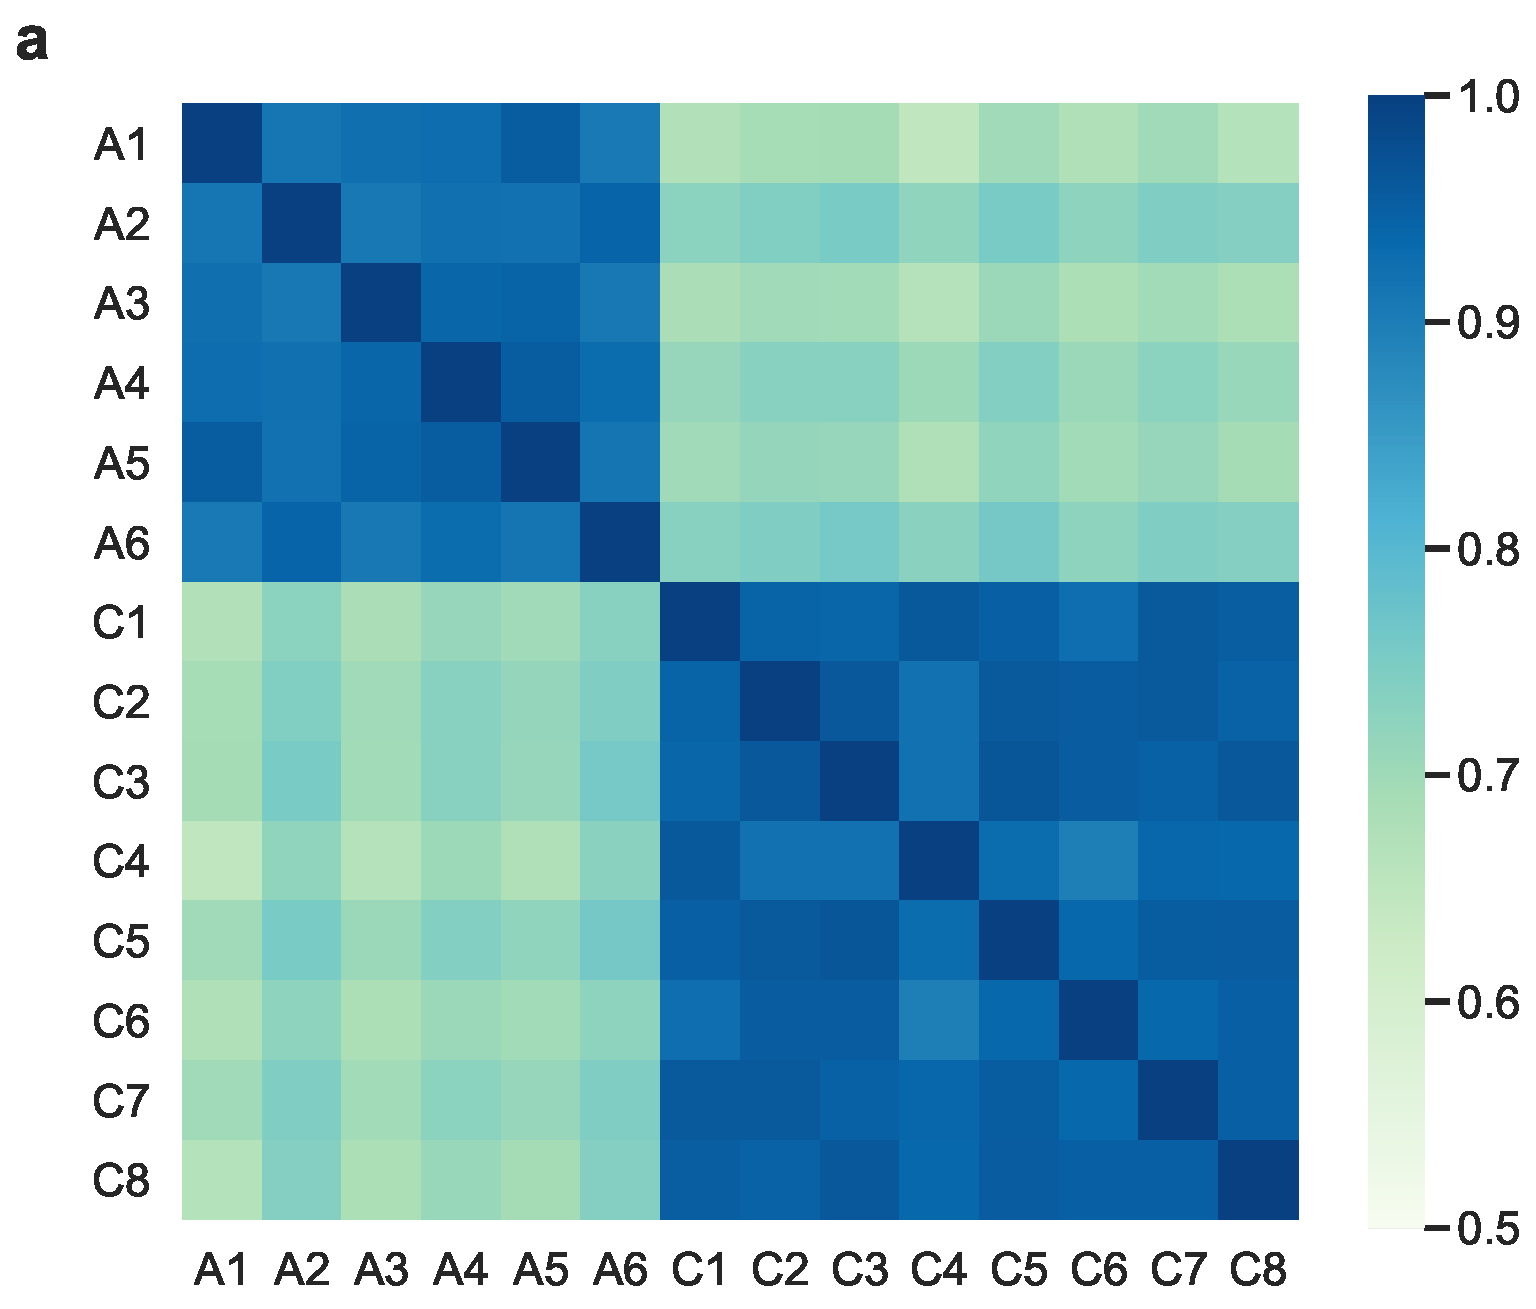
\includegraphics[scale=.3]{chapter2/figures/supfig3a.pdf}\par
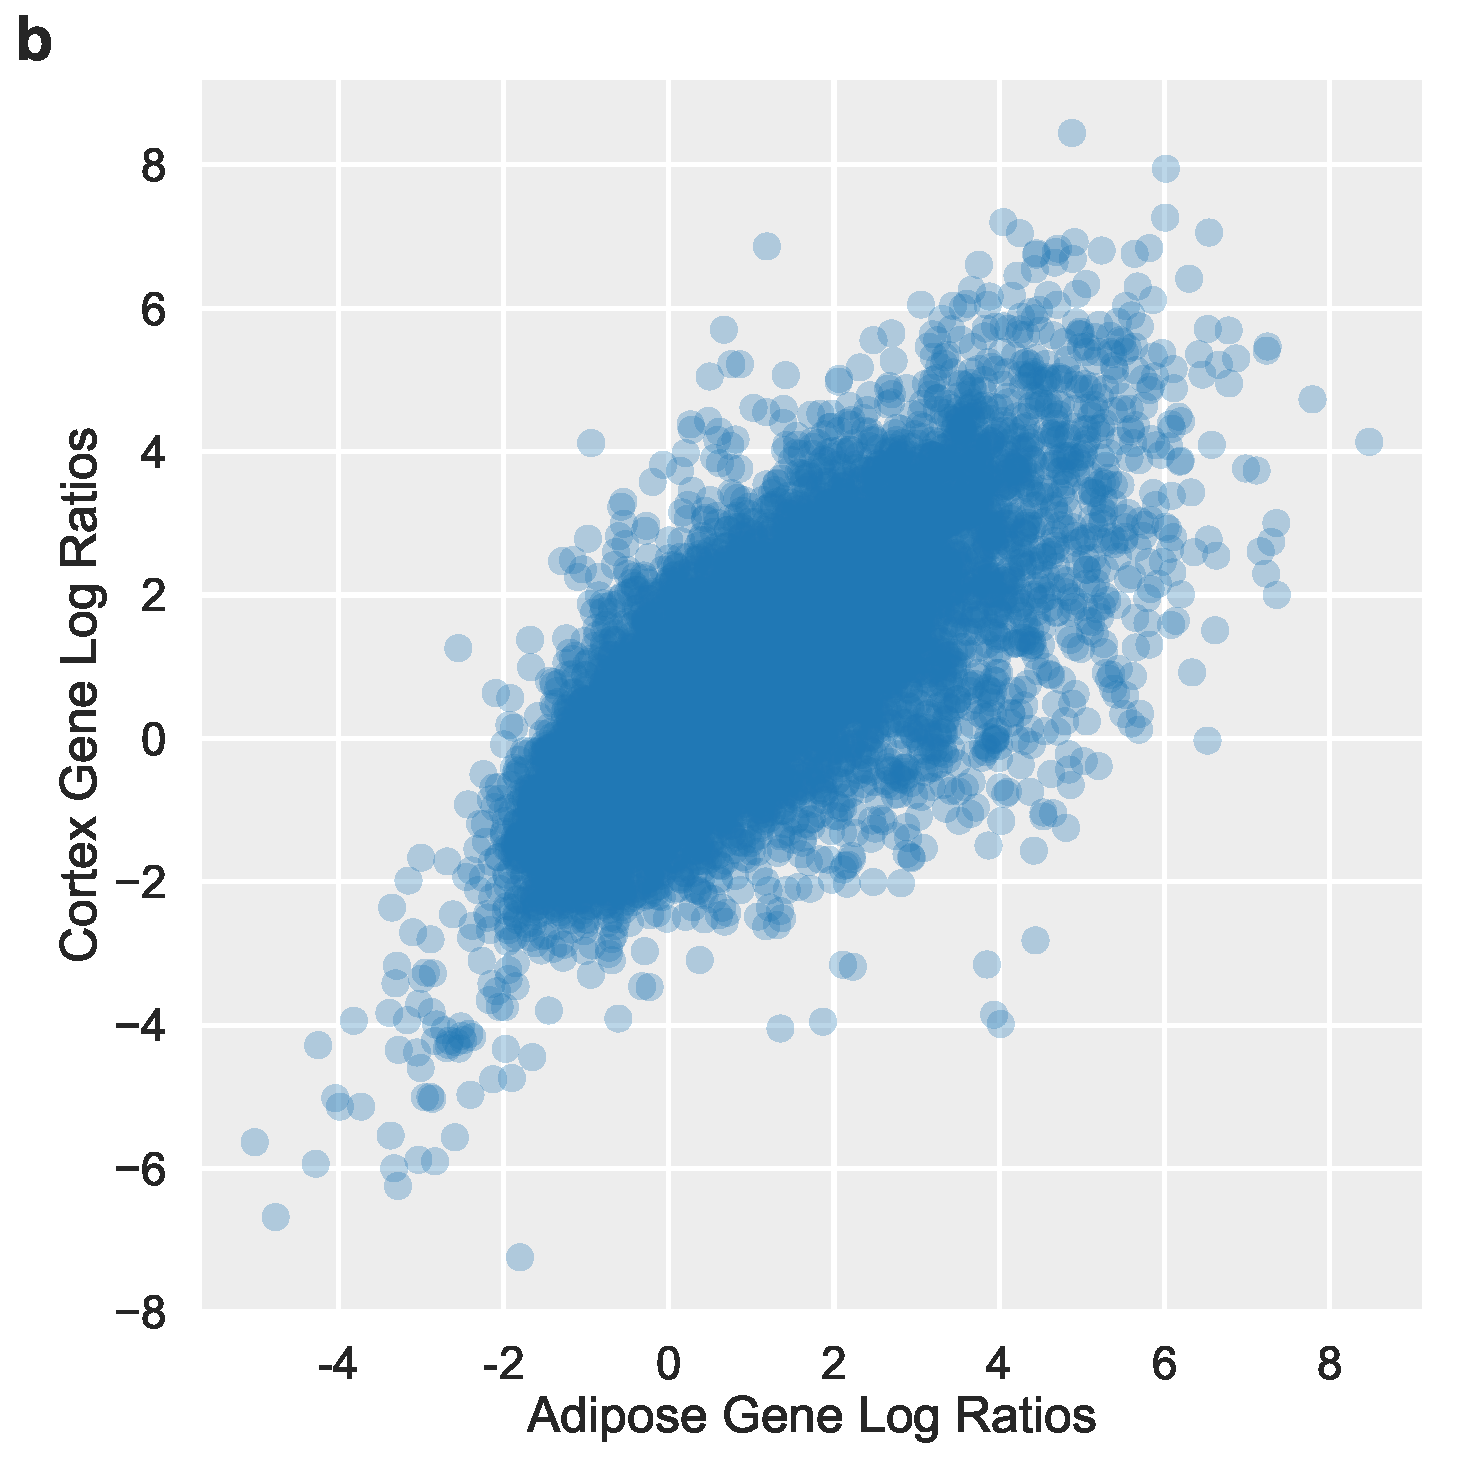
\includegraphics[scale=\figscale]{chapter2/figures/supfig3b.pdf}\par
\end{multicols}
\caption{
        Consistency of snRNA-seq to bulk RNA-seq expression log-ratios across individuals, tissues, and experiments.
        (\textbf{a}) Heatmap depicting Pearson correlation between pairs of individual’s log-ratios of snRNA-seq expression to bulk RNA-seq gene expression measured in counts per million (CPM). A sample prefix of ‘A’ indicates an individual from the adipose dataset and ‘C’ indicates an individual from the cortex dataset. Correlation is high between individuals within experiments as well as between experiments/tissues, indicating the same genes are over/under-expressed in snRNA-seq when compared to bulk RNA-seq.
        (\textbf{b}) Scatterplot of average snRNA-seq to bulk RNA-seq gene expression log-ratios across individuals in adipose dataset (x-axis) and cortex dataset (y-axis). Each point corresponds to a gene detected in both experiments, depicting the average ratio across all individuals for that tissue. The snRNA-seq to bulk RNA-seq ratios vary across genes and correlate (R=0.747) between these two experiments.
        }
\label{fig:supfig2.3}
\end{figure}

We performed simulations based on the adipose snRNA-seq data to demonstrate the effect of technology-based biases between the reference profile and bulk expression on decomposition performance. In these analyses, we benchmarked Bisque and three existing methods (MuSiC, BSEQ-sc, and CIBERSORT). Briefly, we simulated bulk expression for 6 individuals by summing the observed snRNA-seq read counts. To model discordance between the reference and bulk, we applied gene-specific linear transformations of the simulated bulk expression. For each gene, the coefficient and intercept of the linear transformation were sampled from half-normal distributions with increasing variance. In this model, a higher variance corresponds to a larger bias between sequencing experiments. While these transformations closely mirrored the Bisque decomposition model, they utilized the true snRNA-seq counts for each individual whereas Bisque learned these transformations using the reference profile generated from averaging these counts across all cells. Hence, this simulation framework introduced additional noise that Bisque does not entirely model. We evaluated decomposition performance by comparing proportion estimates to the proportions observed in the snRNA-seq data in terms of global Pearson correlation (R) and root mean squared deviation (RMSD). Due to the small number of samples, we applied leave-one-out cross-validation to predict the cell composition of each individual using the remaining snRNA-seq samples as training data for each method. In these simulations, Bisque remained robust (R $\approx$ 0.85, RMSD $\approx$ 0.07) at higher levels of simulated bias between the bulk and snRNA-seq-based reference (Figure \ref{fig:fig2.2}b).

\begin{figure}
    \centering
    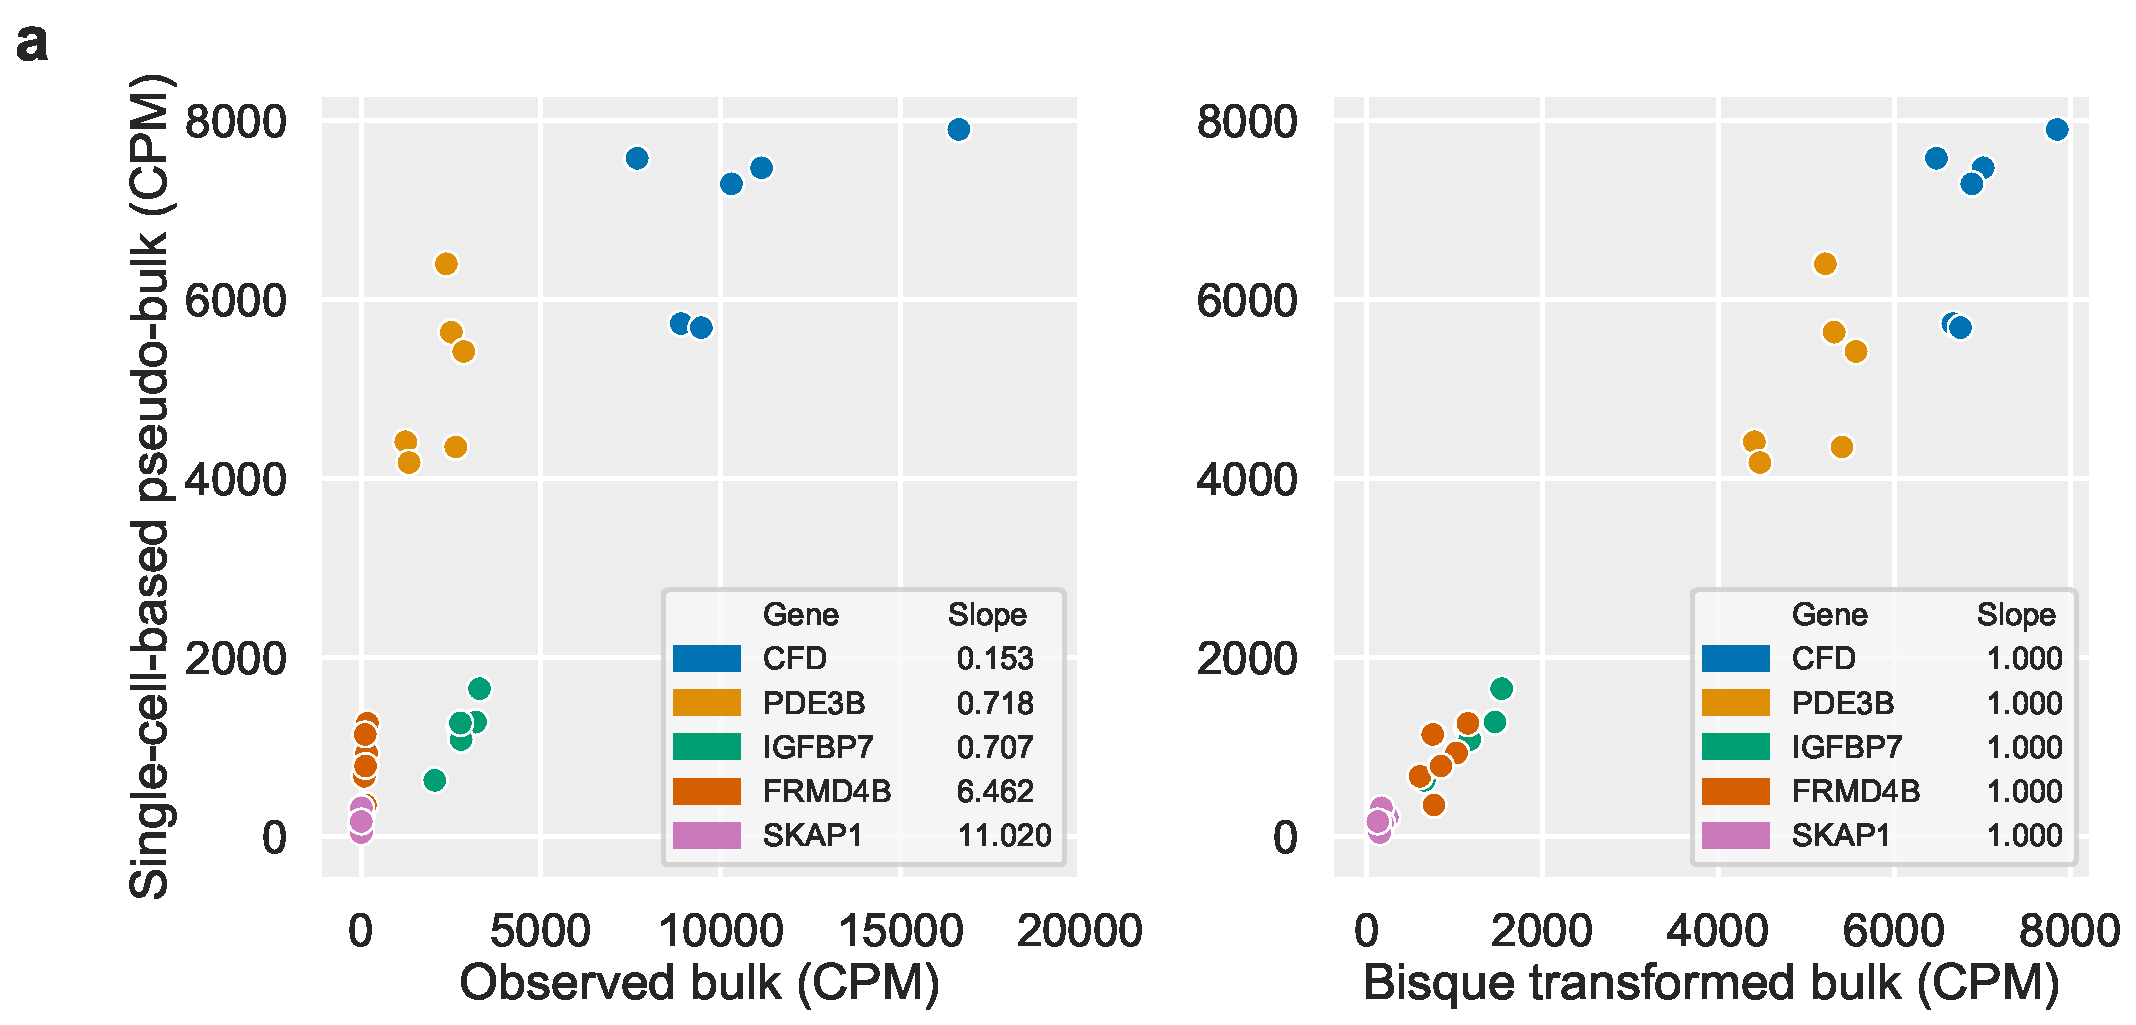
\includegraphics[scale=\figscale]{chapter2/figures/fig2a.pdf} \\[0.25in]
    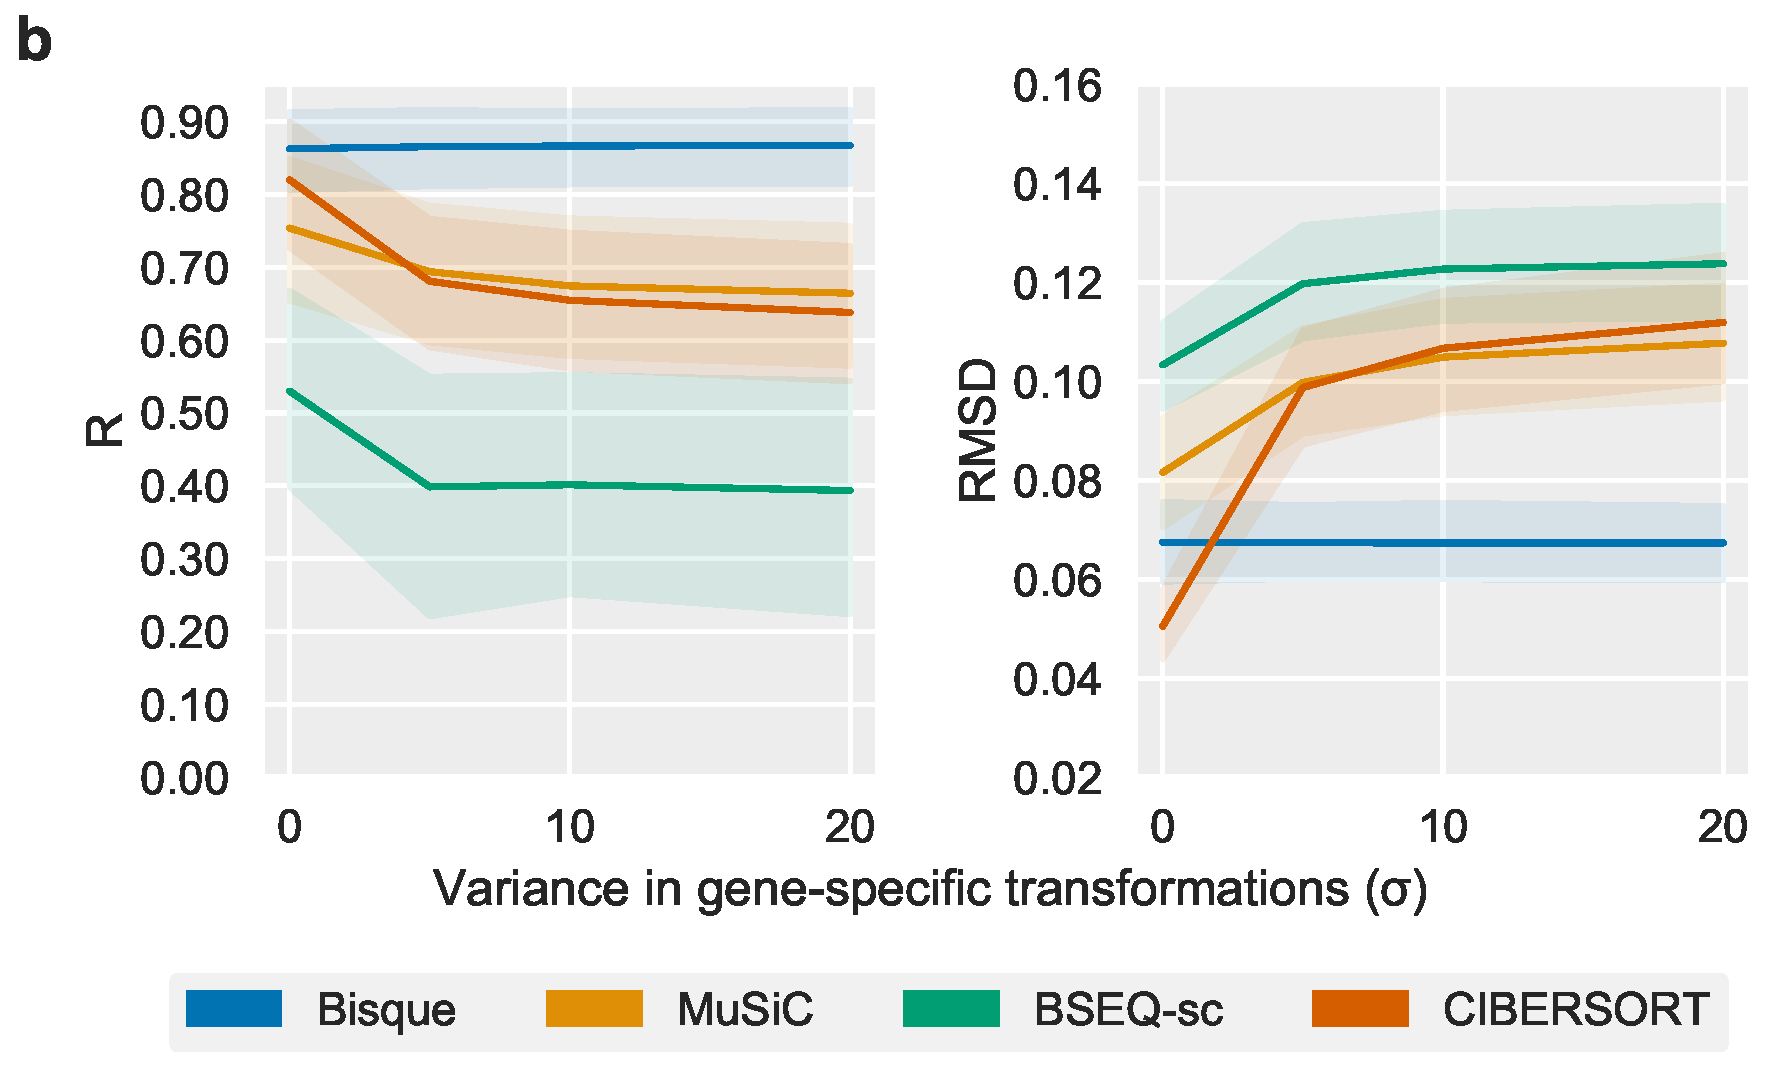
\includegraphics[scale=\figscale]{chapter2/figures/fig2b.pdf}
    \\[0.25in]
    \caption{
             The effect of discrepancies between a single-cell based reference and bulk expression on decomposition. (\textbf{a}) Observed discrepancies in real data between single-nucleus and bulk expression for selected
             marker genes (left) for six individuals. Each color corresponds to a gene. On the left, observed bulk expression on the x-axis is plotted against the pseudo-bulk expression on the y-axis, where pseudo-bulk expression is calculated by summing the single-cell based reference with cell proportions as weights. On the right, the Bisque transformation of bulk expression is on the x-axis. Bisque recovers a one-to-one relationship by transforming the bulk expression 
             for improved decomposition accuracy (right).  
             (\textbf{b}) Simulation of bulk expression for six individuals based on true adipose snRNA-seq data with increasing gene-specific differences. These differences are modeled as a linear transformation of the summed snRNA-seq counts with coefficient and intercept sampled from Half-Normal distributions with parameter as indicated on the x-axis. At $\sigma=0$, the simulated bulk is simply the sum of the observed single-cell read counts. Performance on y-axis measured in global Pearson correlation (R) (left) and root mean squared deviation (RMSD) (right). Shaded regions indicate 95\% confidence intervals based on bootstrapping with central lines indicate the mean observed value. Bisque remains robust to increasing gene-specific variation between single-cell and bulk expression levels.
            }
    \label{fig:fig2.2}
\end{figure}
	 	 	
Next, we performed this cross-validation benchmark on the observed bulk RNA-seq data for these 6 individuals and found that Bisque (R = 0.923, RMSD = 0.074) provided significantly improved global accuracy in detecting each cell type over existing methods (Table \ref{table:table2.2}). MuSiC (R = -0.111, RMSD = 0.427), BSEQ-sc (R = -0.113, RMSD = 0.432), and CIBERSORT (R = -0.131, RMSD = 0.416) severely underestimated the proportion of adipocytes (the most abundant population in adipose tissue) while overestimating the endothelial cell fraction. We also benchmarked CIBERSORTx~\cite{Newman2019-mq}, which employs a batch correction mode to account for biases in sequencing technologies. While CIBERSORTx (R = 0.687, RMSD = 0.099) outperformed existing methods, Bisque provided improved accuracy. It should be noted that cell-specific accuracy is more informative than global R and RMSD; however, these small sample sizes did not provide robust measures of within-cell-type performance in this cross-validation framework. We were able to slightly improve the number of detected cell populations by MuSiC, BSEQ-sc, and CIBERSORT when we considered only snRNA-seq reads aligning to exonic regions of the transcriptome, indicating that intronic reads introduced increasing discrepancy between snRNA-seq and bulk RNA-seq in the context of decomposition. However, given that a significant portion of the nuclear transcriptome consists of pre-mRNA, this filtering process removed over 40 percent of cells detected in the snRNA-seq data. Moreover, Bisque provided improved accuracy over existing methods using this exonic subset of the snRNA-seq data.
\begin{table}
    \scriptsize
    \centering
    \begin{tabular}{|p{3cm}|p{3cm}|p{3cm}|}
    \hline
    \rowcolor{mygray}
    \textbf{Method} & \textbf{R} & \textbf{RMSD} \\ \hline
    Bisque & \textbf{0.923 $\pm$ 0.064} & \textbf{0.074 $\pm$ 0.034} \\ \hline
    CIBERSORTx & 0.687 $\pm$ 0.450 & 0.099 $\pm$ 0.046 \\ \hline
    MuSiC & -0.111 $\pm$ 0.182 & 0.427 $\pm$ 0.058 \\ \hline
    BSEQ-sc & -0.113 $\pm$ 0.180 & 0.432 $\pm$ 0.058  \\ \hline
    CIBERSORT & -0.131 $\pm$ 0.176 & 0.416 $\pm$ 0.059  \\ \hline
    \end{tabular} 
    \captionsetup{justification=raggedright,singlelinecheck=false}
    \caption{
        Leave-one-out cross-validation in subcutaneous adipose using 6 samples with snRNA-seq and bulk RNA-seq data available. Proportions based on snRNA-seq were used as a proxy for the true proportions. Performance measured in Pearson correlation (R) and root-mean-square deviation (RMSD) across all 5 identified cell types in each sample. Reported values were averaged across the 6 samples with standard deviation indicated.
        }
    \label{table:table2.2}
\end{table}


We then applied these decomposition methods to the remaining 100 bulk samples and found that the distribution of cell proportion estimates produced by Bisque were most concordant with the expected distribution inferred from the limited number of snRNA-seq samples and previously reported proportions~\cite{Rosen2014-ae,Glastonbury_undated-kk} (Figure \ref{fig:fig2.3}a). While these benchmarks provided a measure of calibration (i.e. the ability to detect cell populations in expected ranges), they did not provide measurements of cell-specific proportion accuracy across individuals. In order to evaluate cell-specific accuracy, we replicated previously reported associations between cell proportions and measured phenotypes. Specifically, we compared cell proportion estimates from each method to body mass index (BMI) and Matsuda index, a measure of insulin resistance. We measured the significance of these association accounting for age, age-squared, sex, and relatedness.

Obesity is associated with adipocyte hypertrophy, the expansion of the volume of fat cells~\cite{Spalding2008-ey}; thus, we expected a negative association between adipocyte proportion and BMI. Bisque, MuSiC and CIBERSORTx produced adipocyte proportion estimates that replicate this behavior, while BSEQ-sc and CIBERSORT were unable to detect this cell population (Figure \ref{fig:fig2.3}b). The adipocyte proportion estimates produced by Bisque (p = 0.030) and CIBERSORTx (p = 0.001) had a significant negative association with BMI (Table \ref{table:suptable2.1a}). In addition, macrophage abundance has been shown to increase in adipose tissue with higher levels of obesity, concomitant with a state of low grade inflammation~\cite{Weisberg2003-hx}. Each method detected macrophage populations that positively associated with BMI; however, only Bisque (p $<$ 0.001), BSEQ-sc (p = 0.004) and CIBERSORTx (p = 0.049) reached significance (Table \ref{table:suptable2.1b}). 
\begin{table}
    \scriptsize
    \centering
    \begin{tabularx}{\textwidth}{|L|L|L|L|L|L|L|L|}
    \hline
    \rowcolor{mygray}
    \textbf{Method} & \textbf{Spearman Correlation} & \textbf{Spearman p-value} & \textbf{Effect Estimate} & \textbf{Effect Standard Error} & \textbf{Effect t-value} & \textbf{Effect p-value}   \\ \hline
    Bisque & -0.178 & 0.090 & -0.282 & 0.126 & -2.240 & \textbf{0.030}  \\ \hline
    MuSiC & 0.038 & 0.719 & -0.081 & 0.108 & -0.754 & 0.455  \\ \hline
    BSEQ-sc & - & - & - & - & - & -  \\ \hline
    CIBERSORT & - & - & - & - & - & - \\ \hline
    CIBERSORTx & -0.300 & \textbf{0.004} & -0.361 & 0.100 & -3.624 & \textbf{0.001} \\ \hline
    BisqueMarker & -0.227 & \textbf{0.030} & -0.304 & 0.096 & -3.154 & \textbf{0.003}  \\ \hline    
    \end{tabularx}
    \caption{Association of adipocyte proportion with BMI. A negative association was expected.}
    \label{table:suptable2.1a}
\end{table}
\begin{table}
    \scriptsize
    \centering
    \begin{tabularx}{\textwidth}{|L|L|L|L|L|L|L|L|}
    \hline
    \rowcolor{mygray}
    \textbf{Method} & \textbf{Spearman Correlation} & \textbf{Spearman p-value} & \textbf{Effect Estimate} & \textbf{Effect Standard Error} & \textbf{Effect t-value} & \textbf{Effect p-value}   \\ \hline
    Bisque & 0.389 & \textbf{$\mathbf{<}$ 0.001} & 0.460 & 0.099 & 4.671 & \textbf{$\mathbf{<}$ 0.001}  \\ \hline
    MuSiC & 0.065 & 0.540 & 0.034 & 0.110 & 0.308 & 0.760  \\ \hline
    BSEQ-sc & 0.238 & \textbf{0.022} & 0.278 & 0.092 & 3.013 & \textbf{0.004}  \\ \hline
    CIBERSORT & 0.239 & \textbf{0.022} & 0.162 & 0.102 & 1.597 & 0.118 \\ \hline
    CIBERSORTx & 0.273 & \textbf{0.009} & 0.224 & 0.102 & 2.192 & \textbf{0.034} \\ \hline
    BisqueMarker & 0.296 & \textbf{0.004} & 0.253 & 0.103 & 2.465 & \textbf{0.018}  \\ \hline    
    \end{tabularx}
    \caption{Association of macrophage proportion with BMI. A positive association was expected.}
    \label{table:suptable2.1b}
\end{table}

T cells were the least abundant cell type population identified from the snRNA-seq data, constituting around 4 percent of all sequenced nuclei. The abundance of T cells has been observed to positively correlate with insulin resistance~\cite{McLaughlin2014-gn}. Thus, we compared decomposition estimates for T cell proportions to Matsuda index. As a lower Matsuda index indicates higher insulin resistance, we expect a negative association between T cell proportion and Matsuda index. Proportion estimates produced by Bisque and CIBERSORTx followed this trend while the remaining existing methods did not identify T cells in the bulk samples (Figure \ref{fig:fig2.3}c). We found this association significant for Bisque (p $<$ 0.001) and CIBERSORTx (p = 0.047) (Table \ref{table:suptable2.1c}) after correcting for diabetes status, since Matsuda index may not be informative in these individuals~\cite{Gutch2015-db}. 

\begin{table}
    \scriptsize
    \centering
    \begin{tabularx}{\textwidth}{|L|L|L|L|L|L|L|X|}
    \hline
    \rowcolor{mygray}
    \textbf{Method} & \textbf{Spearman Correlation} & \textbf{Spearman p-value} & \textbf{Effect Estimate} & \textbf{Effect Standard Error} & \textbf{Effect t-value} & \textbf{Effect p-value}   \\ \hline
    Bisque & -0.195 & 0.075 & -0.387 & 0.116 & -3.328 &  \textbf{0.002}  \\ \hline
    MuSiC & - & - & - & - & - & -  \\ \hline
    BSEQ-sc & - & - & - & - & - & -  \\ \hline
    CIBERSORT & - & - & - & - & - & - \\ \hline
    CIBERSORTx & -0.317 & \textbf{0.003} & -0.230 & 0.111 & -2.068 & \textbf{0.046} \\ \hline
    BisqueMarker & -0.294 & \textbf{0.007} & -0.188 & 0.100 & -1.874 & 0.069  \\ \hline    
    \end{tabularx}
    \caption{Association of T cell proportion with Matusda index, a measure of insulin resistance. A negative association was expected. An additional covariate accounting for diabetes status was added to the LMM due to previously reported significant associations with Matsuda index.}
    \label{table:suptable2.1c}
\end{table}

\begin{figure}
\centering
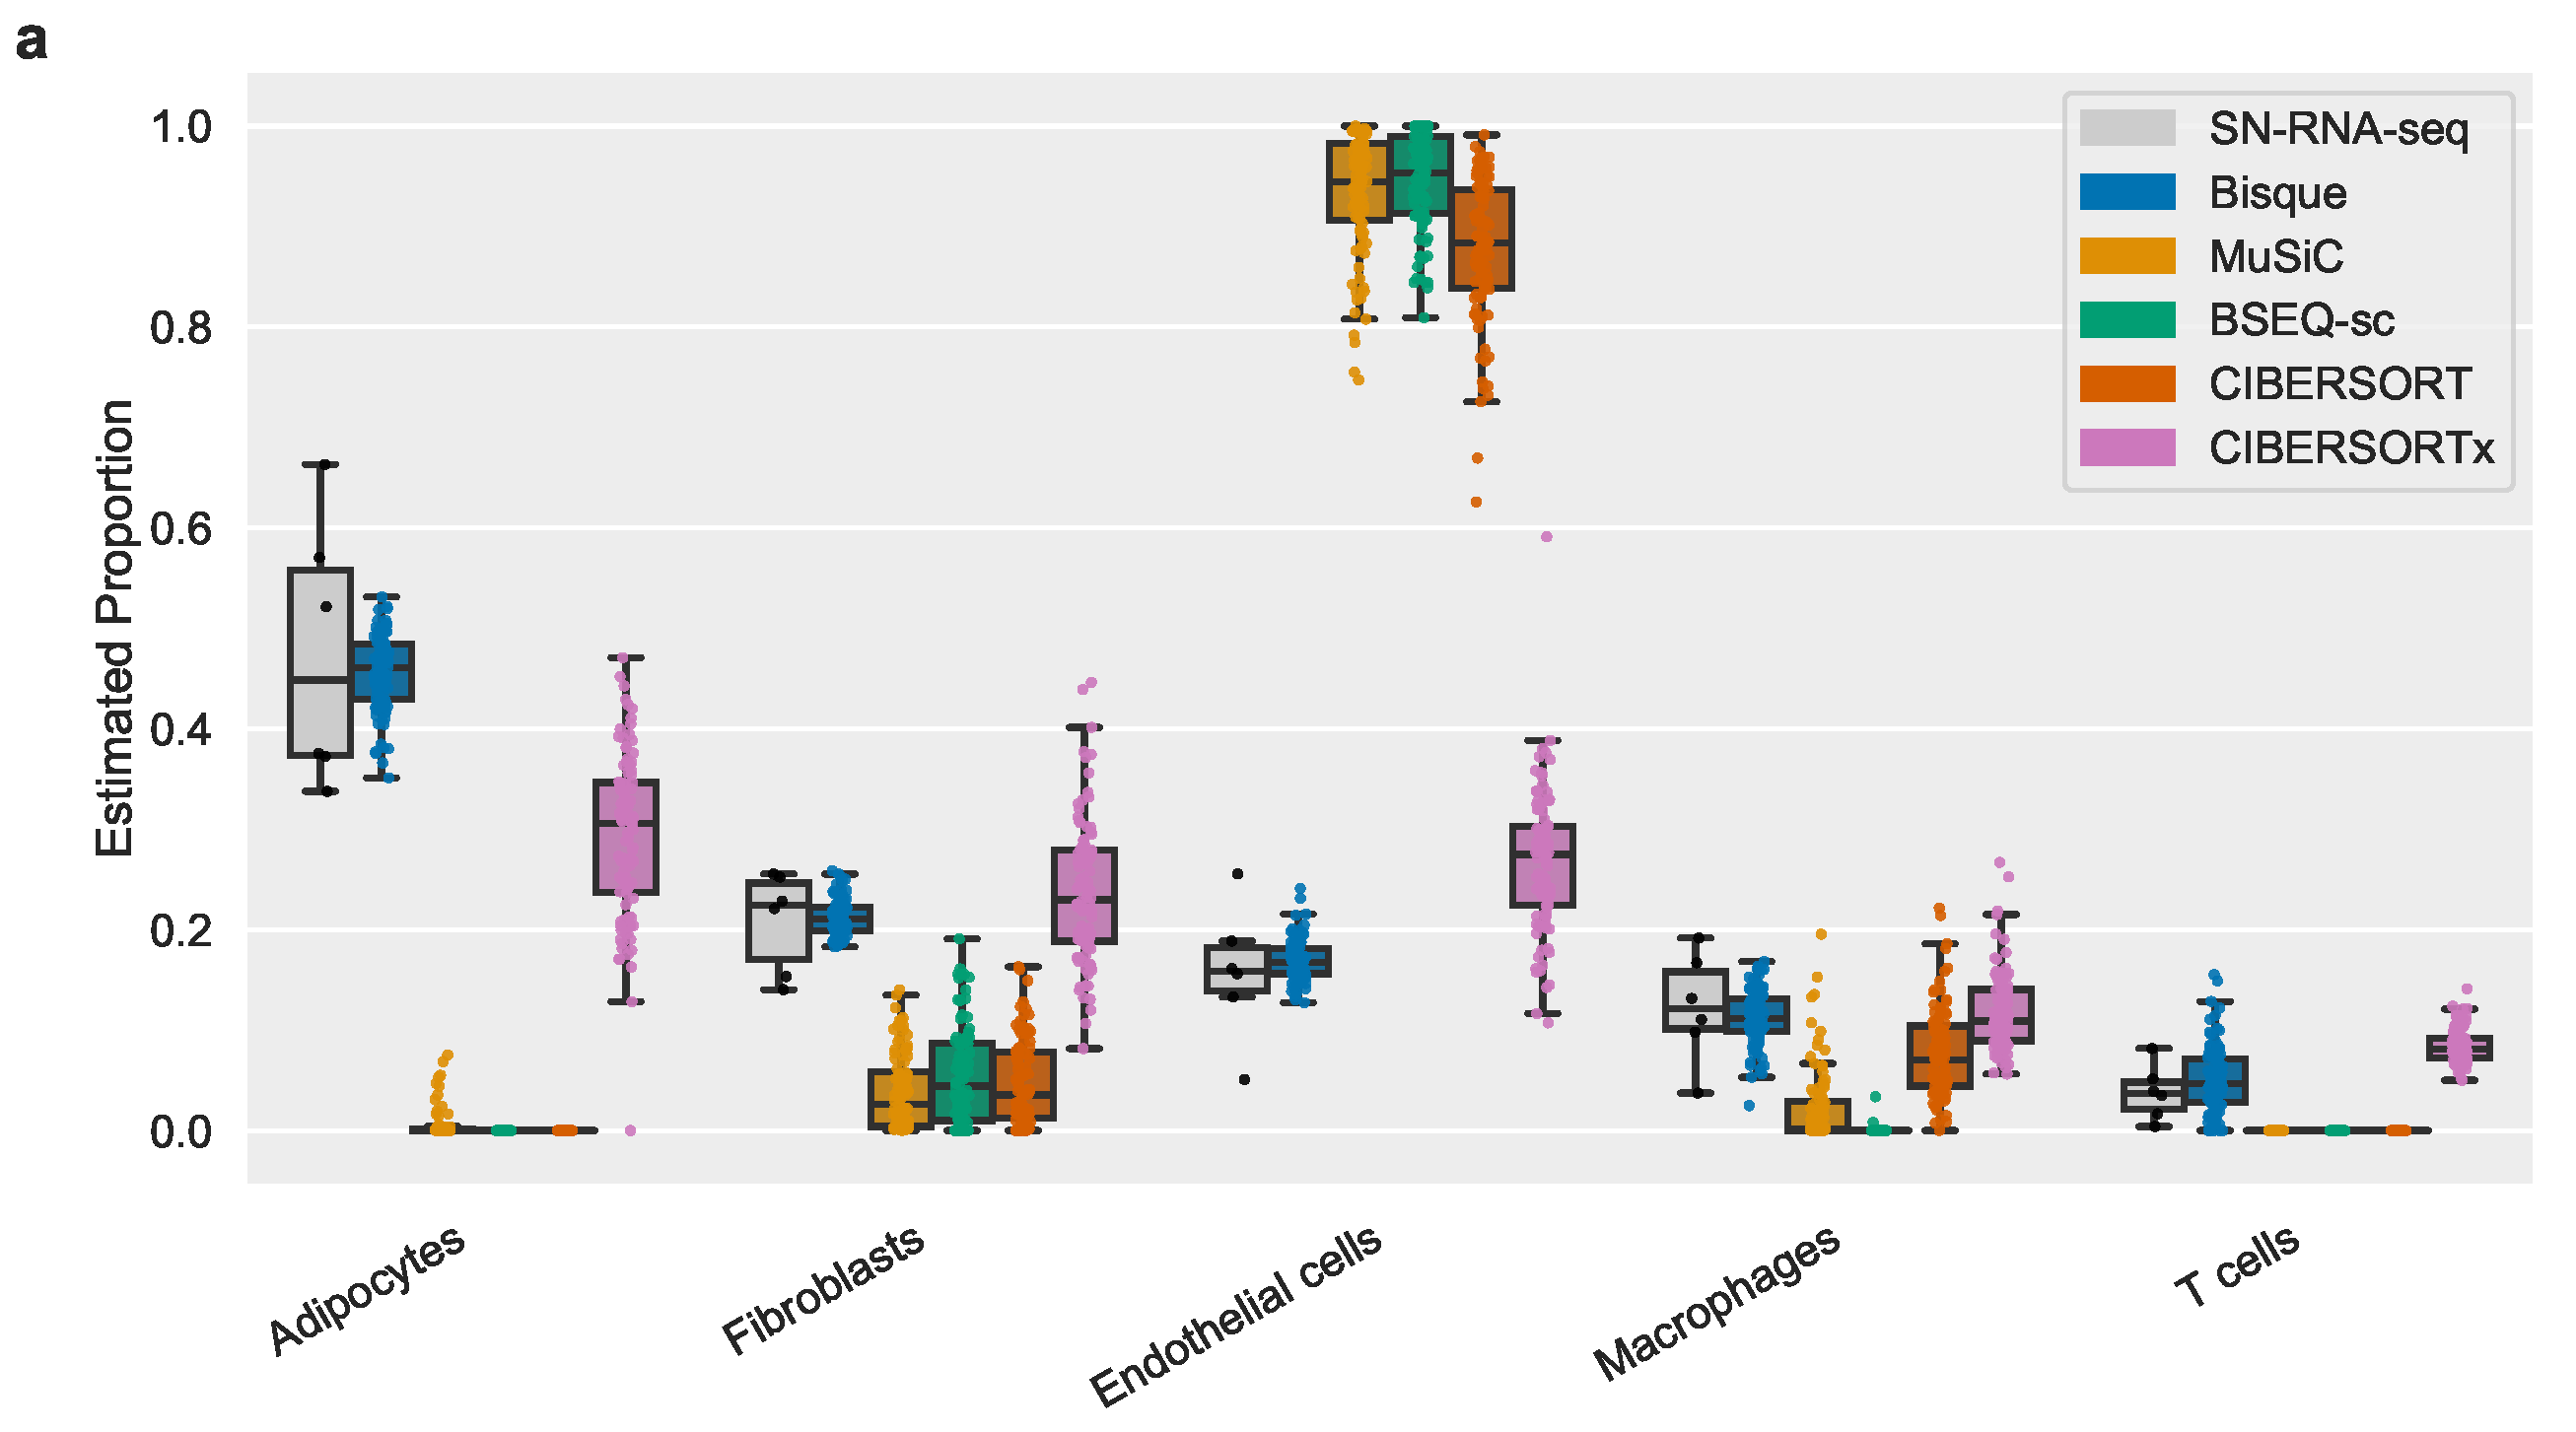
\includegraphics[scale=\figscale]{chapter2/figures/fig3a.pdf}
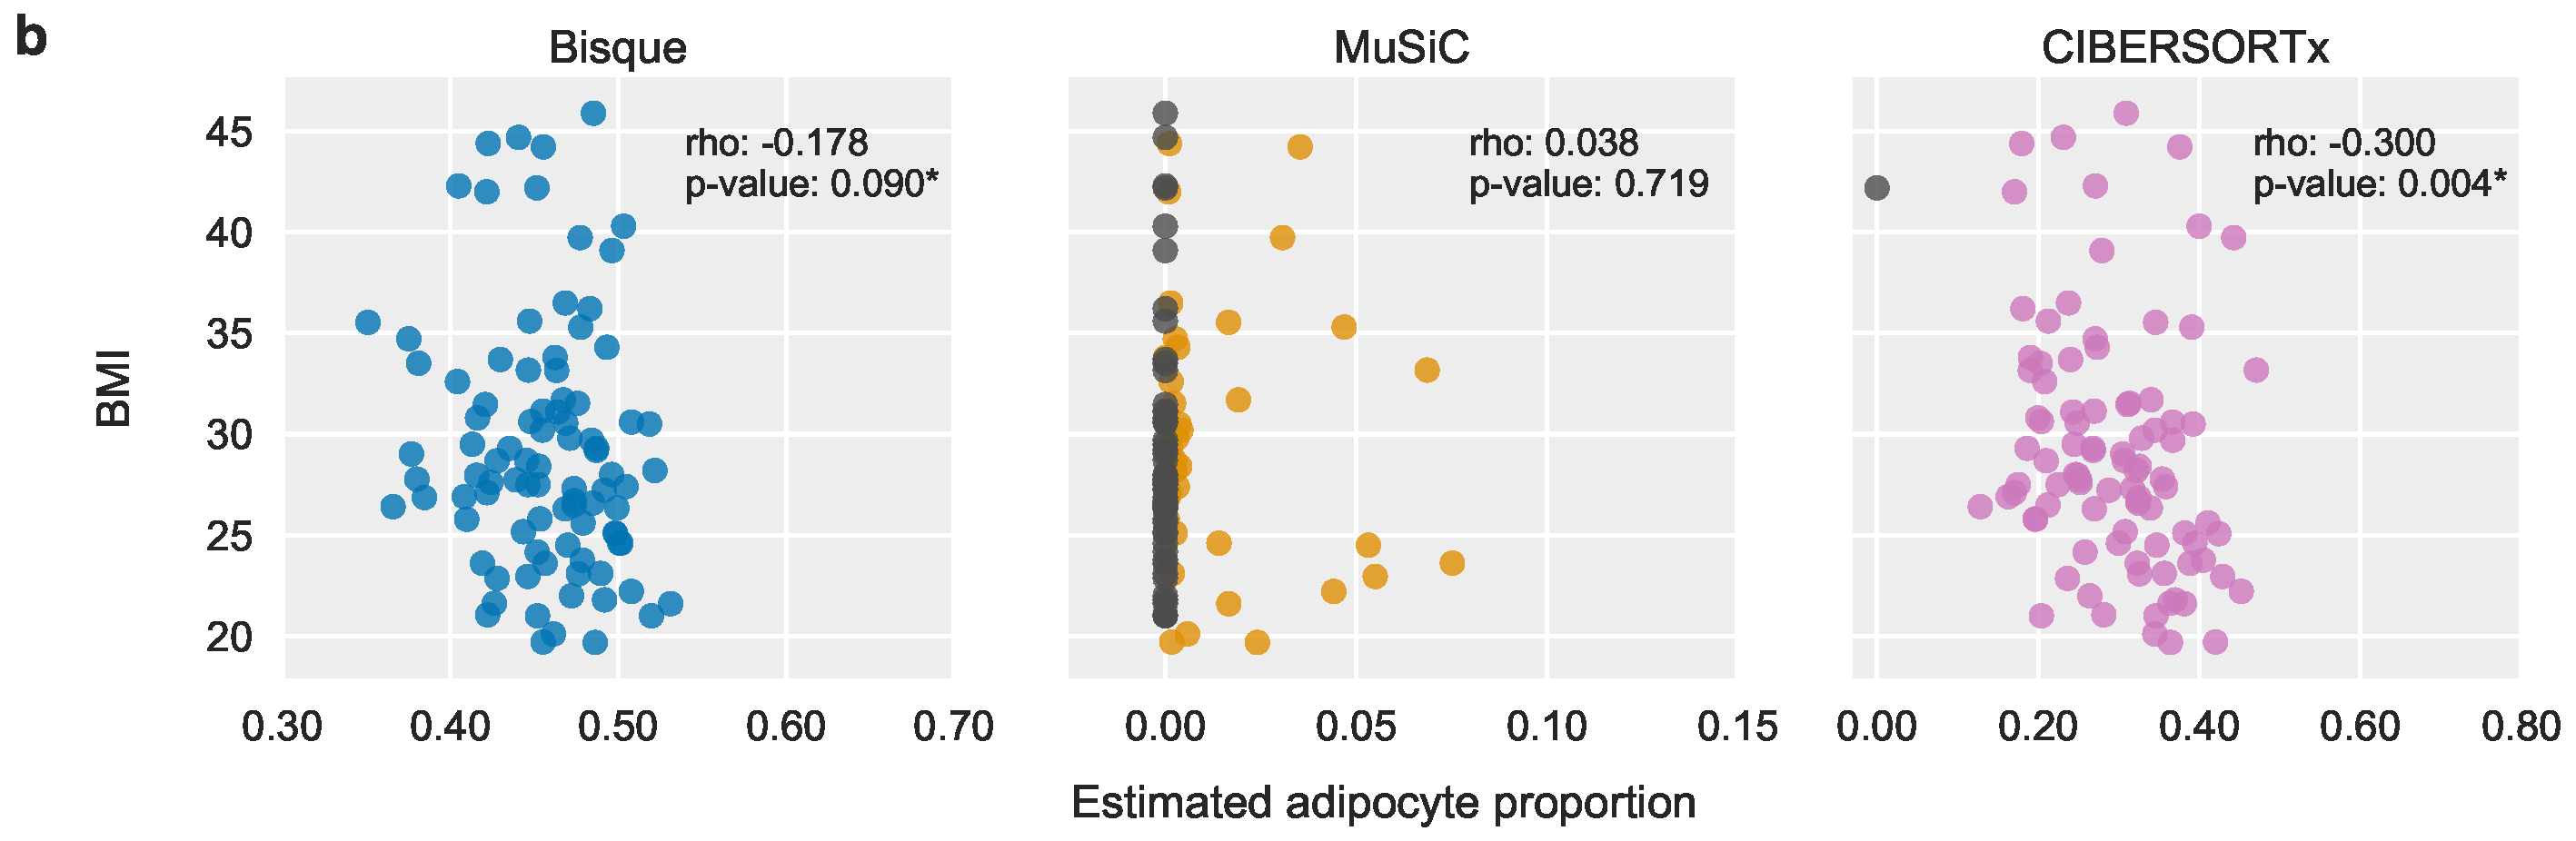
\includegraphics[scale=\figscale]{chapter2/figures/fig3b.pdf}
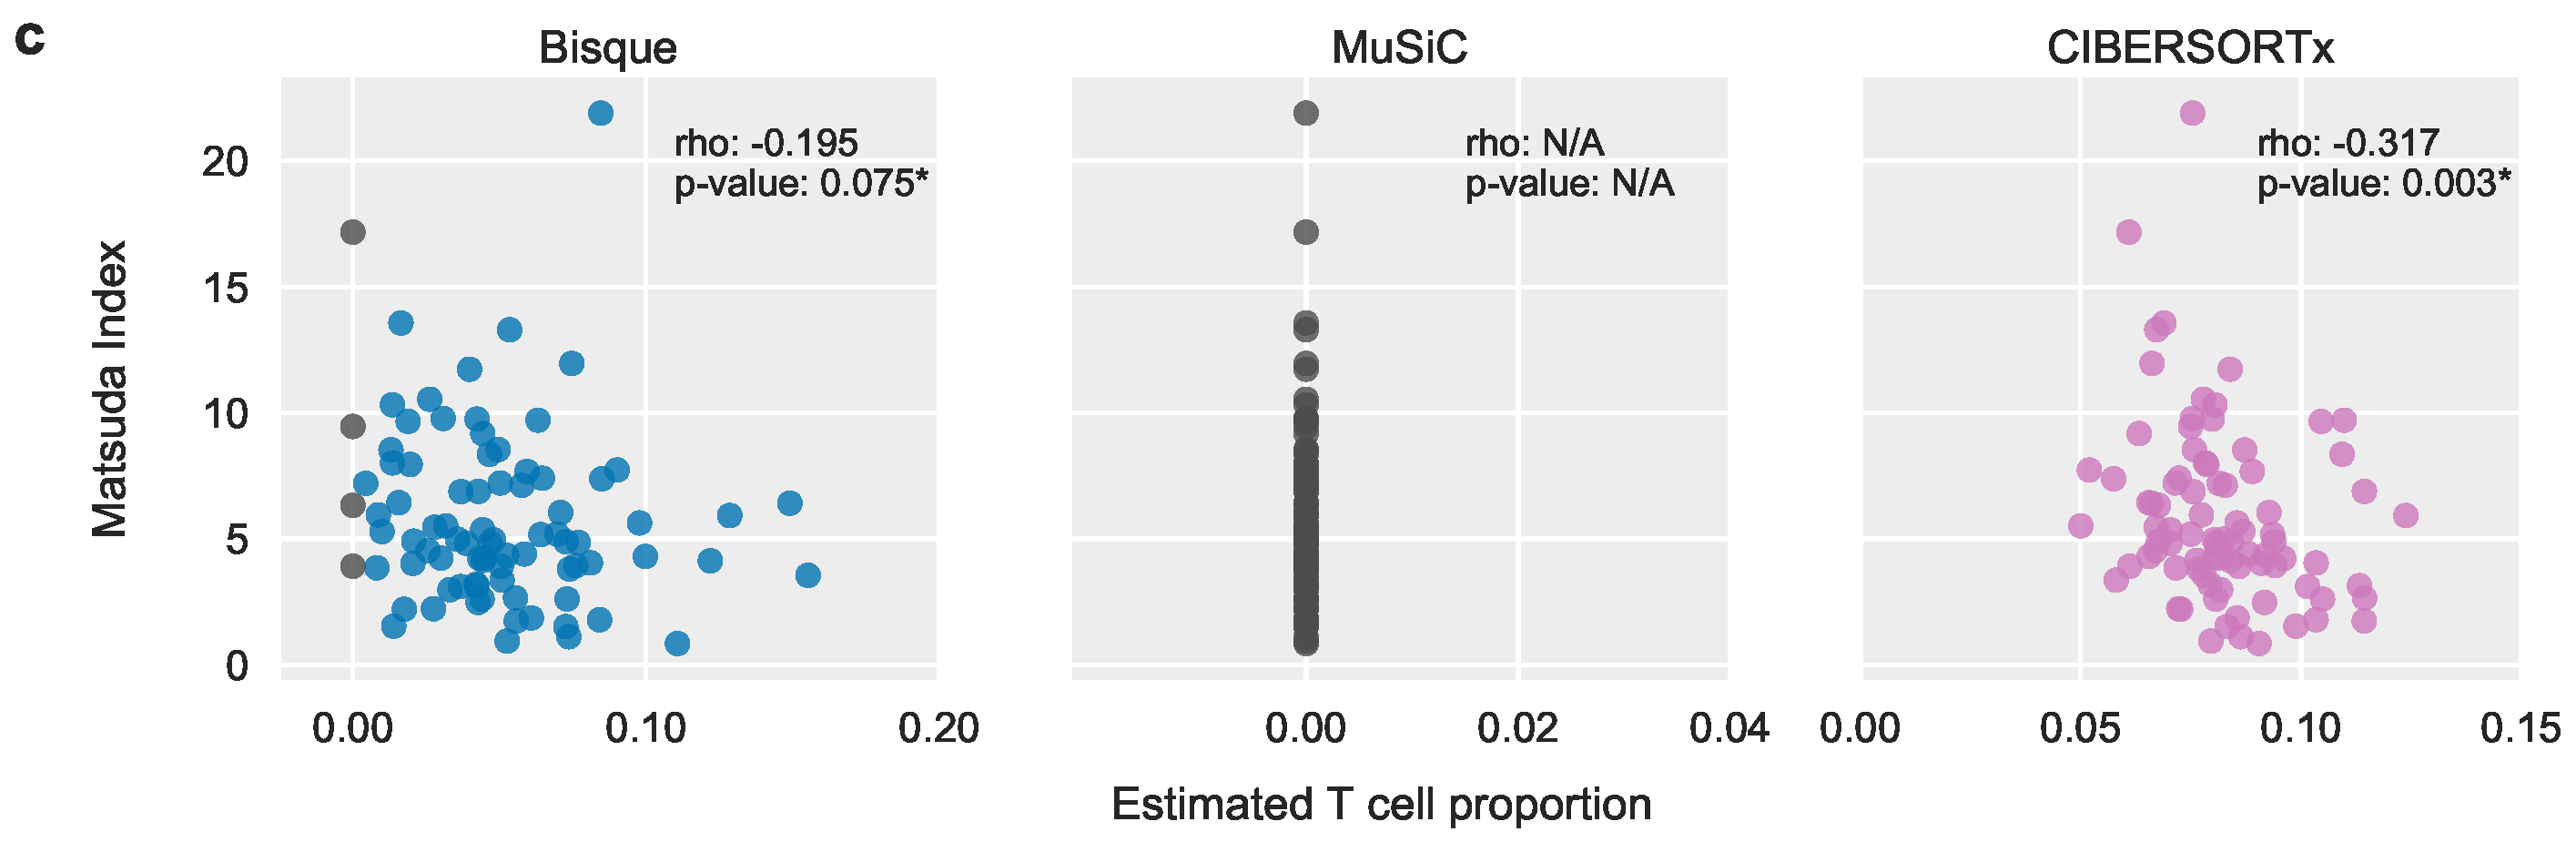
\includegraphics[scale=\figscale]{chapter2/figures/fig3c.pdf}
\caption{
         Decomposition benchmark in human subcutaneous adipose tissue.
         (\textbf{a}) Comparison of decomposition estimates from 100 individuals with estimates from 6 individuals with snRNA-seq data available. 
         (\textbf{b-c}) Scatterplots comparing decomposition estimates with measured phenotypes in 100 individuals. Reported ‘rho’ corresponds to Spearman correlation and p-values indicate the significance of these correlations, with an asterisk denoting significance after correction for covariates (sex, age, age-squared, and relatedness). CIBERSORT and BSEQ-sc are not shown since they did not detect these cell populations.
         (\textbf{b}) Adipocyte proportion has been observed to negatively correlate with BMI so we expected a negative correlation.
         (\textbf{c}) T cell proportion has previously been reported to positively correlate with insulin resistance. Matsuda index decreases with higher insulin resistance so we expected a negative correlation.
        }
\label{fig:fig2.3}
\end{figure}

\subsection{Evaluation of decomposition performance in cortex tissue}

We also benchmarked these decomposition methods using expression data collected from the dorsolateral prefrontal cortex (DLPFC). This dataset was generated by the Rush Alzheimer’s Disease (AD) Center~\cite{Mostafavi2018-ch}  and includes 636 postmortem bulk RNA-seq samples. The Religious Orders Study and Rush Memory and Aging Project were approved by an IRB of Rush University Medical Center. Both bulk RNA-seq and snRNA-seq data were collected from 8 of the individuals (Table \ref{table:table2.1}). Using the same pipeline we used to process the adipose dataset, we identified 11 clusters: 3 neuronal subtypes, 2 interneuronal subtypes, 2 astrocyte subtypes, oligodendrocytes, oligodendrocyte progenitor cells, and microglia (Figure \ref{fig:supfig2.1}b). We observed a higher overlap in marker genes for these clusters than in those identified in the adipose dataset (average of 10\% of marker genes shared between clusters in DLPFC compared to 3\% in adipose).
 	
We again applied leave-one-out cross-validation on the 8 individuals with both RNA-seq and snRNA-seq data available. In this example, randomly sampled 25\% of the nuclei in the snRNA-seq data to accommodate CIBERSORTx (which is currently web-based and restricts the size of files that can be processed). Bisque was able to detect each cell population identified from the snRNA-seq data with high global accuracy (R = 0.924, RMSD = 0.029) while MuSiC (R = -0.192, RMSD = 0.173), BSEQ-sc (R = 0.098, RMSD = 0.120), and CIBERSORT (R = -0.281, RMSD = 0.197) did not detect a number of cell populations (Table \ref{table:table2.3}). Bisque also provided higher accuracy than CIBERSORTx (R = 0.671, RMSD = 0.070). However, we found that the performance of the existing methods improved when estimates with subtypes were summed together. While each method was able to quantify major cell populations after merging subtypes, Bisque was able to distinguish between these closely related cell populations. Interestingly, we found that in both adipose and DLPFC, endothelial cell proportions were overestimated by each of the existing methods.

\begin{table}
    \scriptsize
    \centering
    \begin{tabular}{|p{3cm}|p{3cm}|p{3cm}|}
    \hline
    \rowcolor{mygray}
    \textbf{Method} & \textbf{R} & \textbf{RMSD} \\ \hline
        Bisque & \textbf{0.924 $\pm$ 0.062} & \textbf{0.029 $\pm$ 0.010} \\ \hline
        CIBERSORTx & 0.671 $\pm$ 0.153 & 0.070 $\pm$ 0.019 \\ \hline
        MuSiC & -0.192 $\pm$ 0.107 & 0.173 $\pm$ 0.013 \\ \hline
        BSEQ-sc & 0.098 $\pm$ 0.216 & 0.120 $\pm$ 0.023 \\ \hline
        CIBERSORT & -0.281 $\pm$ 0.049 & 0.197 $\pm$ 0.012 \\ \hline
    \end{tabular} 
    \captionsetup{justification=raggedright,singlelinecheck=false}
    \caption{
        Leave-one-out cross-validation in dorsolateral prefrontal cortex using 8 samples with snRNA-seq and bulk RNA-seq data available. Proportions based on snRNA-seq were used as a proxy for the true proportions. Performance measured in Pearson correlation (R) and root-mean-square deviation across all 11 identified cell types in each sample. Reported values were averaged across the 8 samples with standard deviation indicated.
        }
    \label{table:table2.3}
\end{table}
We applied these decomposition methods to the remaining 628 individuals and compared the distribution of estimates to the proportions observed in the 8 snRNA-seq samples. We found that Bisque was able to detect each cell population and produced estimates that were closest in mean to the snRNA-seq observations (Figure \ref{fig:fig2.4}a). The increased accuracy of Bisque over existing methods persisted when we merged closely related subtypes. Moreover, immunohistochemistry (IHC) analyses on 70 of these samples found similar proportions of major cell populations~\cite{Patrick_undated-vv}, confirming the relative accuracy of snRNA-seq based estimates of cell proportions. 

\begin{figure}
\centering
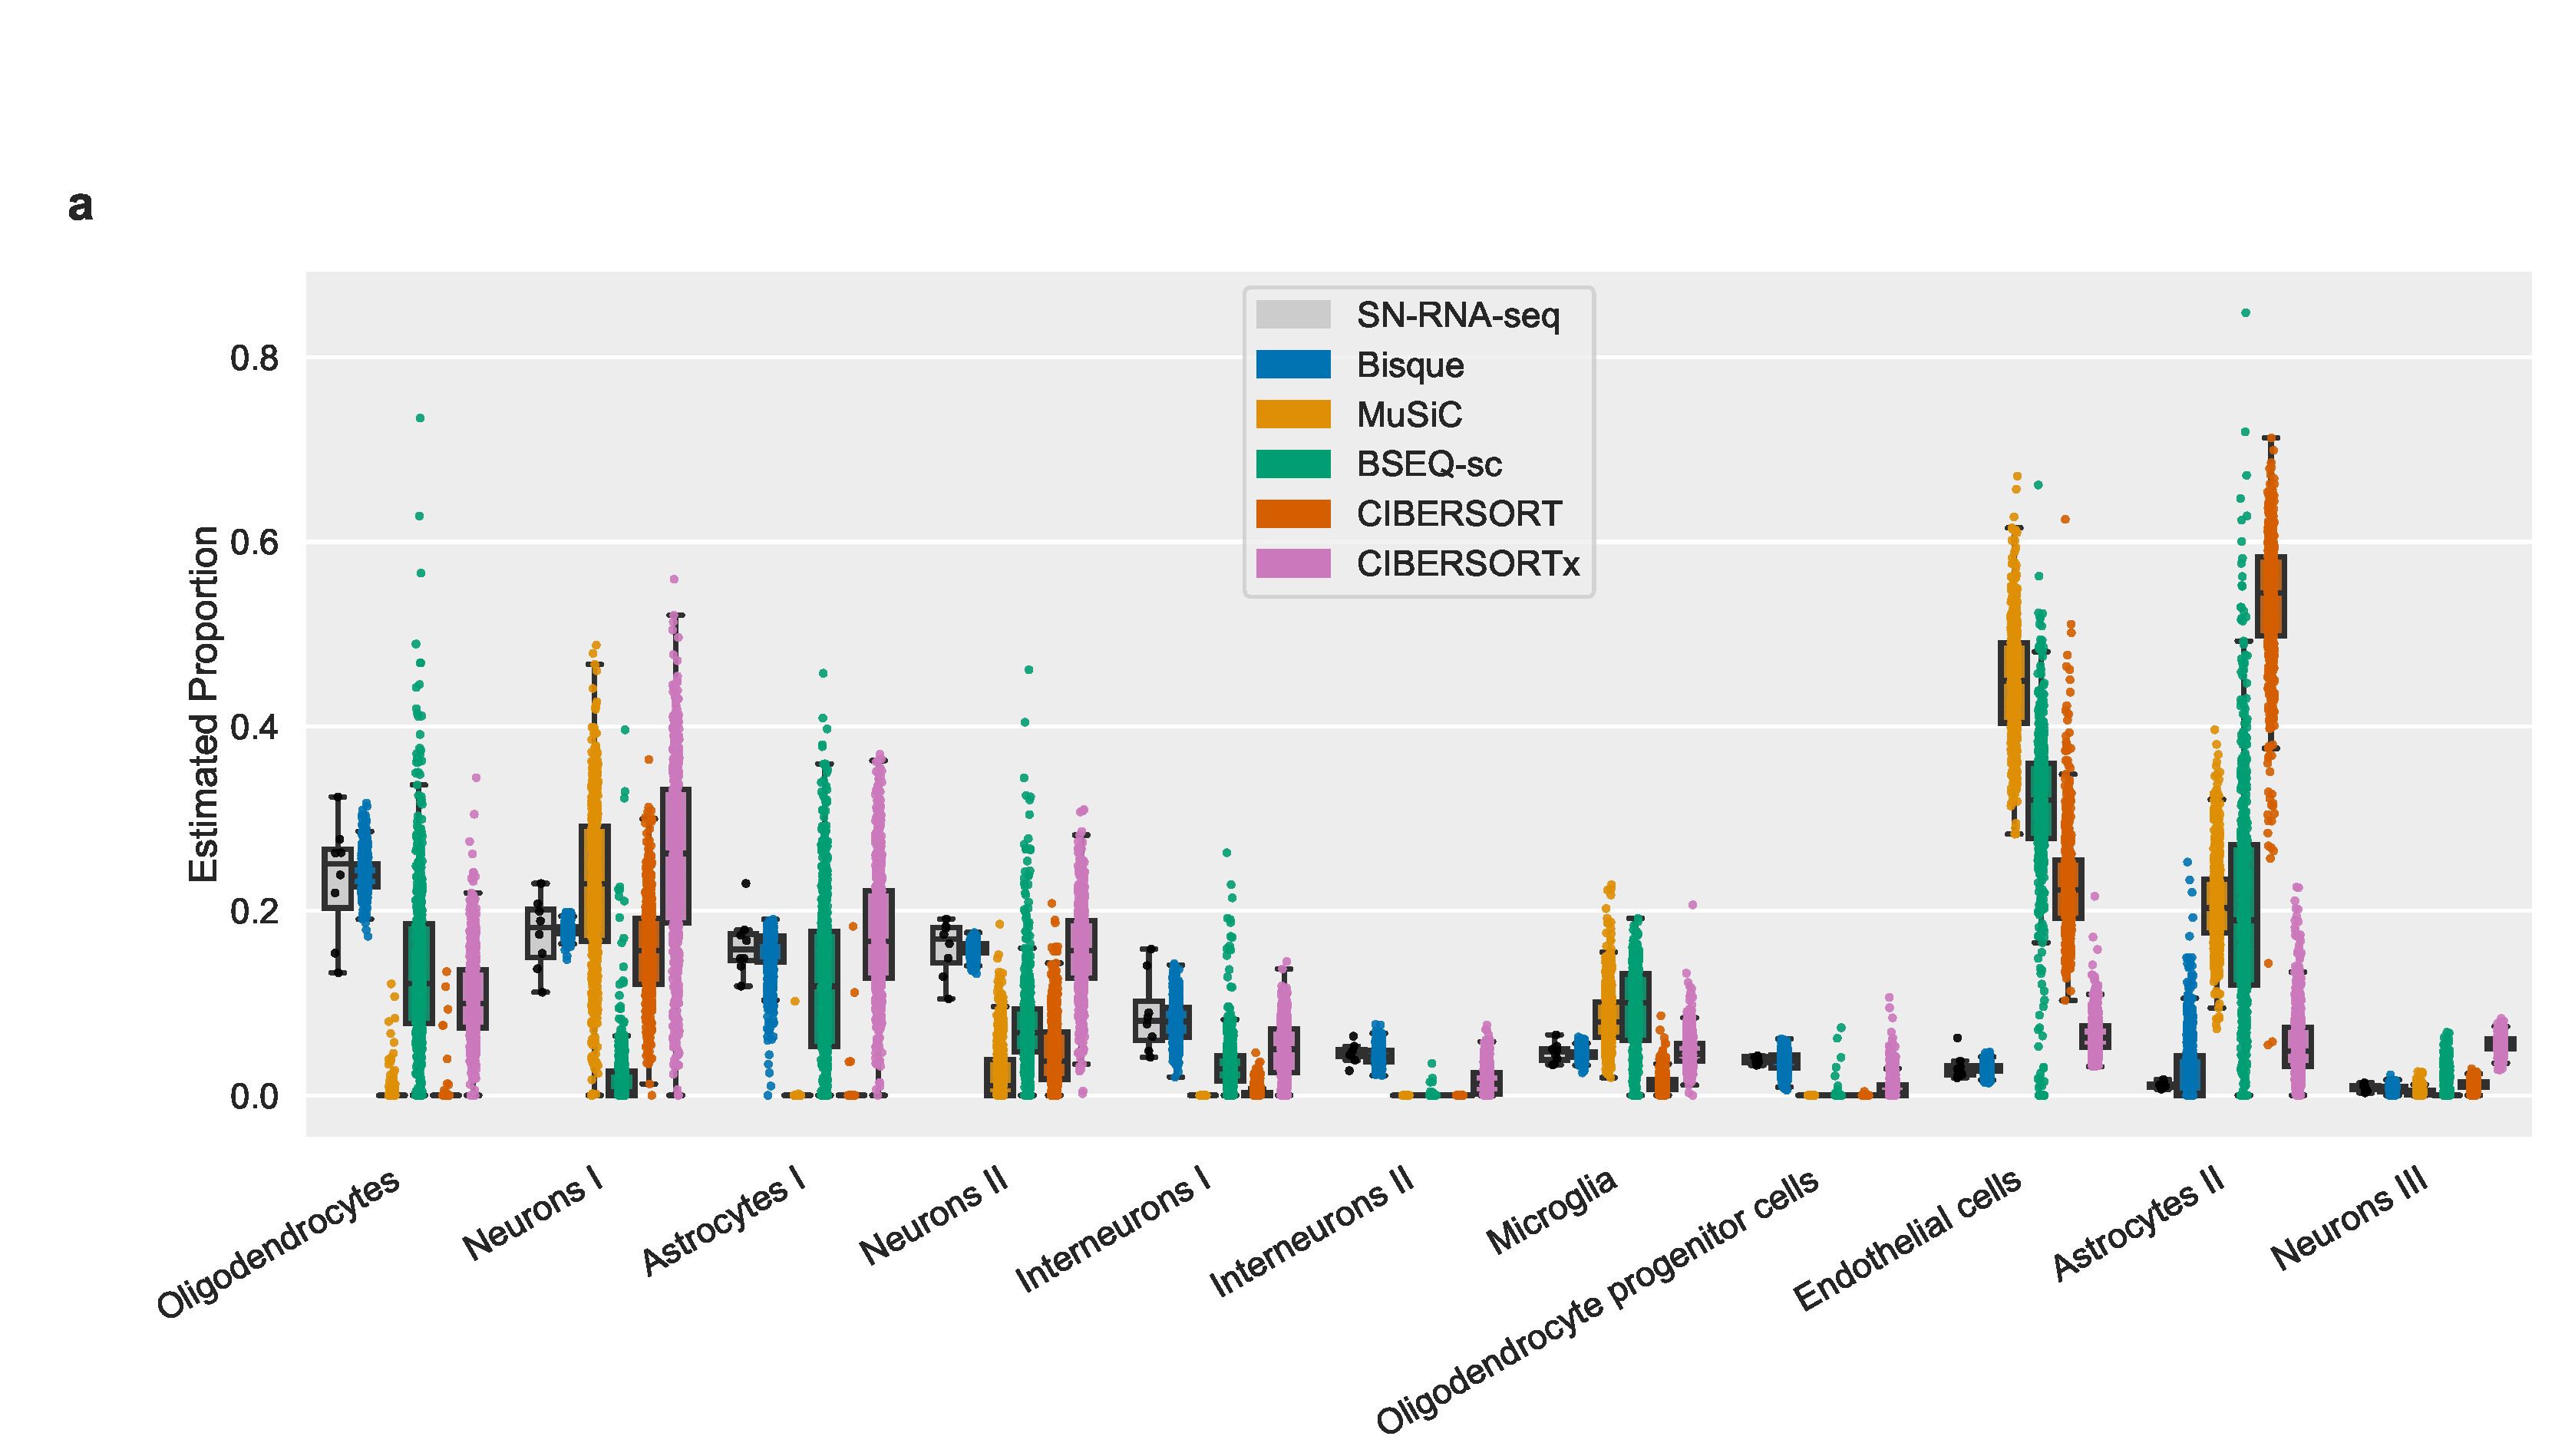
\includegraphics[scale=.24]{chapter2/figures/fig4a.pdf}
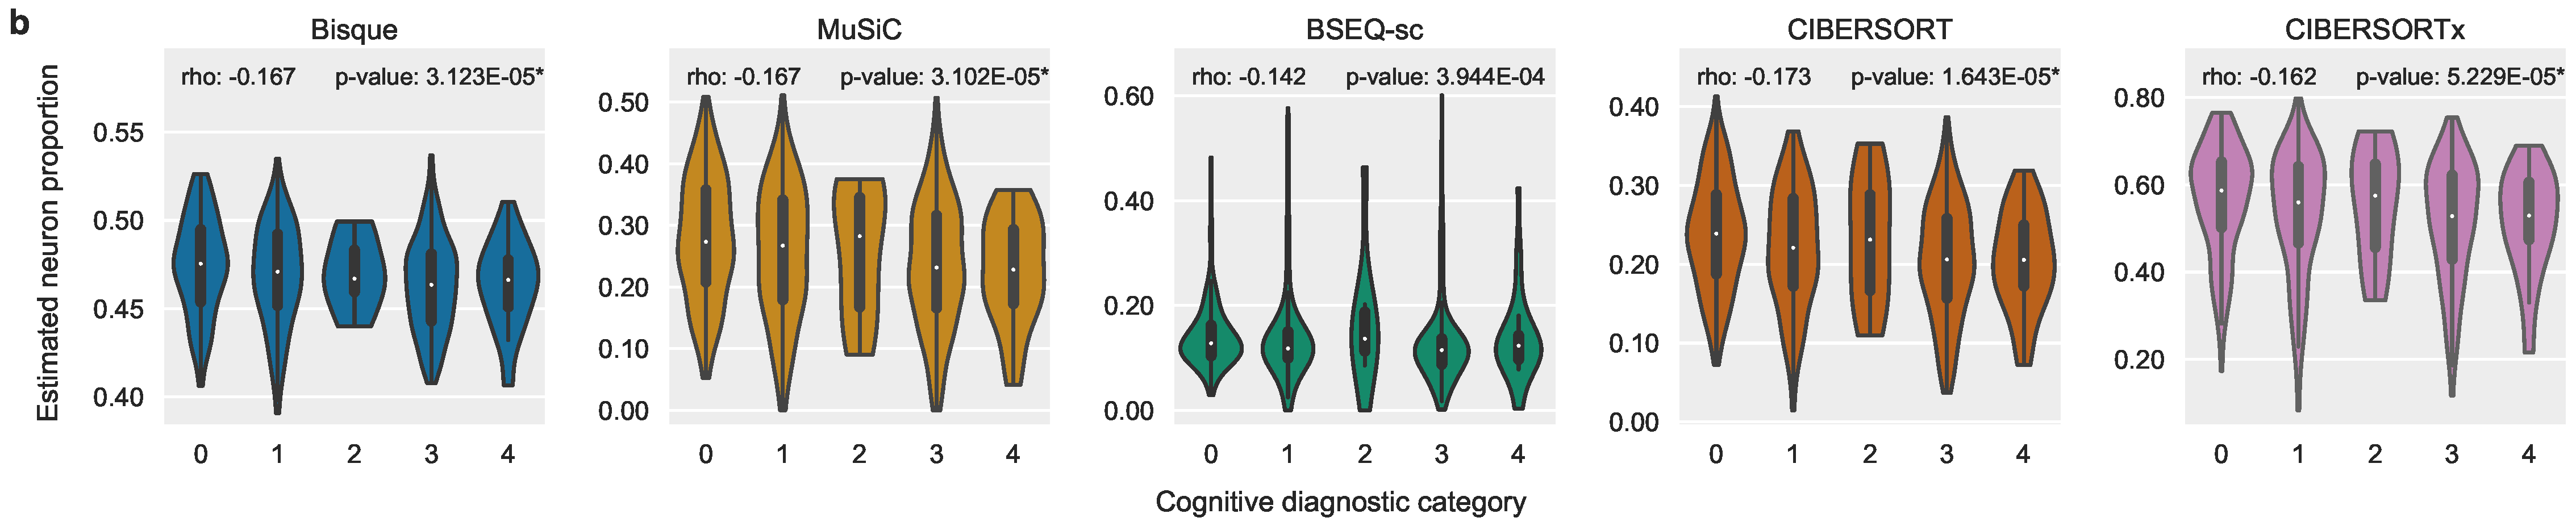
\includegraphics[width=\textwidth]{chapter2/figures/fig4b.pdf}
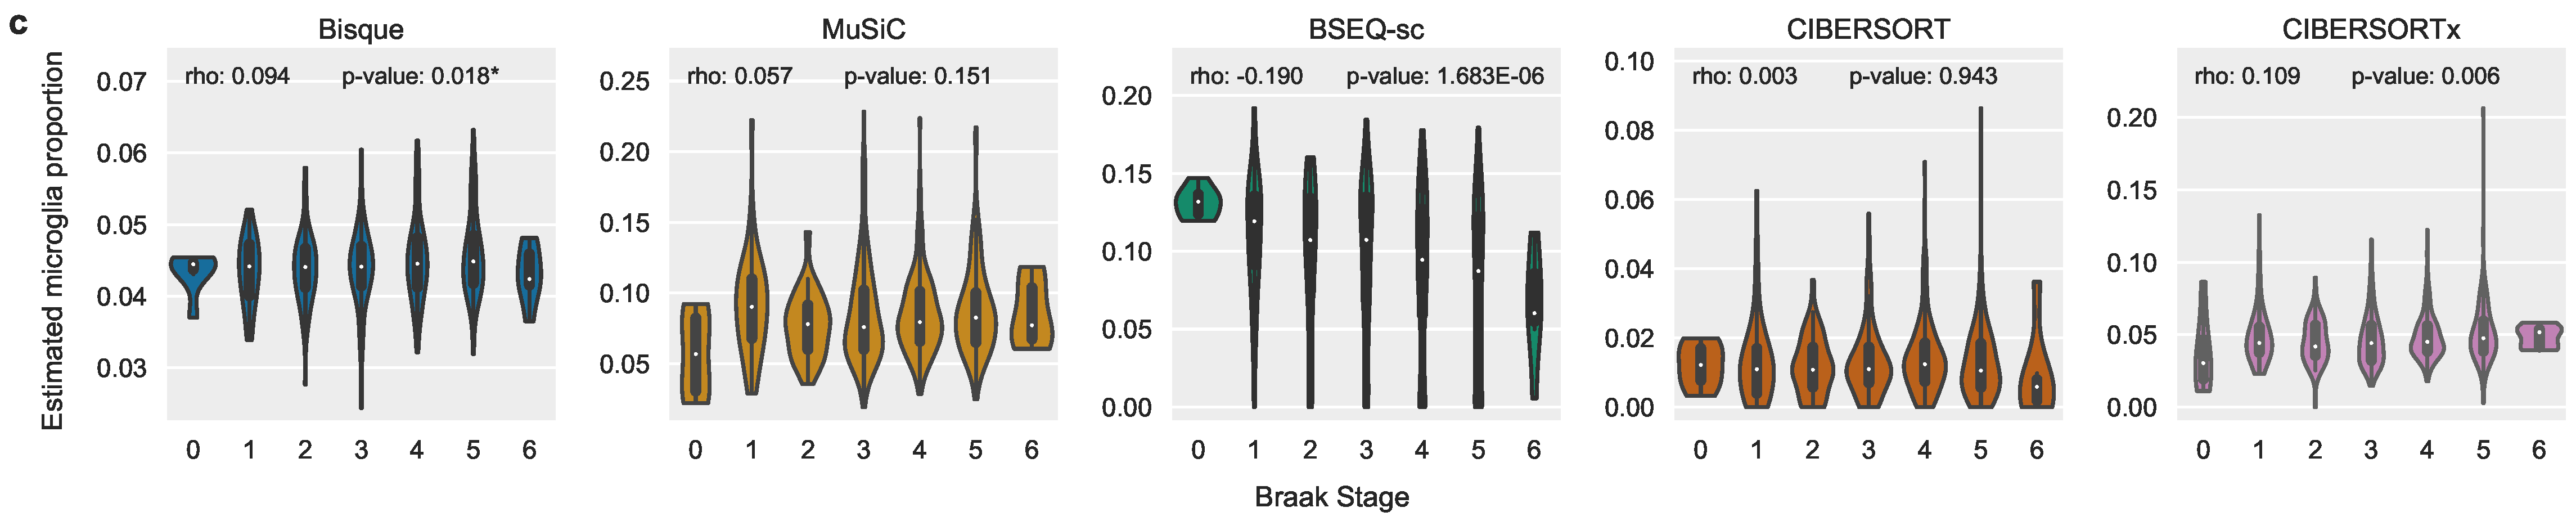
\includegraphics[width=\textwidth]{chapter2/figures/fig4c.pdf}
\caption{
    Decomposition benchmark in human dorsolateral prefrontal cortex tissue.
    (\textbf{a}) Comparison of decomposition estimates from 628 individuals with estimates from 8 individuals with snRNA-seq data available.
    (\textbf{b-c}) Violin plots depicting association of decomposition estimates aggregated into major cell types with measured phenotypes in 628 individuals. Reported ‘rho’ corresponds to Spearman correlation and p-values indicate the significance of these correlations, with an asterisk denoting both an expected effect direction and significance after correction for covariates.
    (\textbf{b}) Neuronal degeneration has been observed in patients diagnosed with Alzheimer’s disease (AD). Cognitive diagnostic category measures a physician’s diagnosis of cognitive impairment (CI), with 0 indicating no CI and 4 indicating a confident AD diagnosis. We expected a negative correlation between neuron proportion and cognitive diagnostic category.
    (\textbf{c}) Microglia proportion has been observed to positively correlate with increased severity of AD symptoms, such as neurofibrillary tangles. Braak stage provides a semiquantitative measure of tangle severity, so we expected an overall positive correlation between microglia proportion and Braak stage.
    }
\label{fig:fig2.4}
\end{figure}

\begin{table}[!ht]
    \scriptsize
    \centering
    \begin{tabularx}{\textwidth}{|L|L|L|L|L|L|L|X|}
    \hline
    \rowcolor{mygray}
    \textbf{Method} & \textbf{Spearman Correlation} & \textbf{Spearman p-value} & \textbf{Effect Estimate} & \textbf{Effect Standard Error} & \textbf{Effect t-value} & \textbf{Effect p-value}   \\ \hline
    Bisque & -0.167 & \textbf{$\mathbf{<}$ 0.001} & -0.145 & 0.039 & -3.705 &  \textbf{$\mathbf{<}$ 0.001}  \\ \hline
    MuSiC & -0.167 & \textbf{$\mathbf{<}$ 0.001} & -0.147 & 0.039 & -3.742 &  \textbf{$\mathbf{<}$ 0.001}  \\ \hline
    BSEQ-sc & -0.142 & \textbf{$\mathbf{<}$ 0.001} & -0.053 & 0.039 & -1.341 & 0.180  \\ \hline
    CIBERSORT & -0.173 & \textbf{$\mathbf{<}$ 0.001} & -0.155 & 0.039 & -3.971 & \textbf{$\mathbf{<}$ 0.001} \\ \hline
    CIBERSORTx & -0.162 & \textbf{$\mathbf{<}$ 0.001} & -0.127 & 0.039 & -3.237 & \textbf{0.001} \\ \hline
    BisqueMarker & -0.141 & \textbf{$\mathbf{<}$ 0.001} & -0.142 & 0.039 & -3.645 & \textbf{$\mathbf{<}$ 0.001}  \\ \hline    
    \end{tabularx}
    \caption{Association of neuron proportion with cognitive diagnosis category. A negative association was expected.}
    \label{table:suptable2.2a}
\end{table}
\begin{table}
    \scriptsize
    \centering
    \begin{tabularx}{\textwidth}{|L|L|L|L|L|L|L|X|}
    \hline
    \rowcolor{mygray}
    \textbf{Method} & \textbf{Spearman Correlation} & \textbf{Spearman p-value} & \textbf{Effect Estimate} & \textbf{Effect Standard Error} & \textbf{Effect t-value} & \textbf{Effect p-value}   \\ \hline
    Bisque & 0.094 & \textbf{0.018} & 0.118 & 0.037 & 3.220 &  \textbf{0.001}  \\ \hline
    MuSiC & 0.057 & 0.151 & 0.019 & 0.037 & 0.509 & 0.611  \\ \hline
    BSEQ-sc & -0.190 & $<$ 0.001 & -0.166 & 0.037 & -4.525 & $<$ 0.001  \\ \hline
    CIBERSORT & 0.003 & 0.943 & -0.005 & 0.037 & -0.137 & 0.891 \\ \hline
    CIBERSORTx & 0.109 & \textbf{0.006} & 0.056 & 0.037 & 1.517 & 0.130 \\ \hline
    BisqueMarker & 0.092 & \textbf{0.021} & 0.054 & 0.037 & 1.444 & 0.149  \\ \hline    
    \end{tabularx}
    \caption{Association of microglia proportion with Braak stage, a measure of neurofibrillary tangles. A positive association was expected.}
    \label{table:suptable2.2b}
\end{table}

Again, to determine cell-specific decomposition accuracy, we replicated known associations between cell type proportions and measured phenotypes in the 628 individuals. For these analyses, we compared cell proportion estimates to each individual’s Braak stage and physician cognitive diagnostic category at time of death. Braak stage is a semiquantitative measure of neurofibrillary tangles, ranging in value from 0 to 5 with increasing severity. The cognitive diagnostic category provides a semiquantitative measure of dementia severity, where a code of 1 indicates no cognitive impairment and 5 indicates a confident diagnosis of AD by physicians.  We determined the significance of these associations based on t-values estimated by a linear regression model that accounted for age, age-squared, and sex. 

Neuronal death is a hallmark symptom of AD~\cite{Yankner1996-lk}. Therefore, we expected to find a negative association between cognitive diagnosis and neuron proportion. We found that each decomposition method provides estimates of total neuron proportion that tend to decrease with cognitive diagnostic category (Figure \ref{fig:fig2.4}b). Each method generates proportions with negative association with cognitive diagnosis. Each method, excluding BSEQ-sc, reached significance in this model (p $\leq$ 0.003 for each method) (Table \ref{table:suptable2.2a}). As another example, we compared each individual’s Braak stage to their estimated proportion of microglia, a relatively small cell population that constituted roughly 5 percent of the sequenced nuclei. Microglia activation has been observed to increase with AD severity~\cite{Hansen2018-jj}. We used Braak stage as a proxy for AD severity and expected a positive association between microglia proportion and Braak stage. Bisque and MuSiC provided estimates that follow this expected trend (Figure \ref{fig:fig2.4}c). Only Bisque produced estimates with a significant positive association (p = 0.001) (Table \ref{table:suptable2.2b}). Interestingly, we observe a decrease in microglia proportions estimated by Bisque in Braak stage 6 individuals which has been previously observed in AD patients~\cite{Navarro2018-ti}.



\subsection{Runtime comparisons of reference-based decomposition methods}

Given the large amounts of transcriptomic data that are becoming available, we also benchmarked these decomposition methods in terms of runtime. In the subcutaneous adipose dataset, which included 100 bulk RNA-seq samples and 6 snRNA-seq samples with about 1,800 nuclei sequenced per individual, Bisque was able to estimate cell proportions efficiently compared to existing methods. Bisque (1 second) and MuSiC (1 second) provided decomposition estimates faster than BSEQ-sc (26 seconds), CIBERSORT (27 seconds), and CIBERSORTx (389 seconds) (Figure \ref{fig:fig2.5}a).  Bisque also provided improved efficiency in processing the reduced DLPFC dataset, which included 628 bulk RNA-seq samples and 8 snRNA-seq samples with around 2,125 nuclei per individual. Bisque (4 seconds) and MuSiC (10 seconds) estimated cell proportions relatively quickly compared to BSEQ-sc (273 seconds), CIBERSORT (298 seconds), and CIBERSORTx (6,566 seconds) (Figure \ref{fig:fig2.5}b).

\begin{figure}
\centering
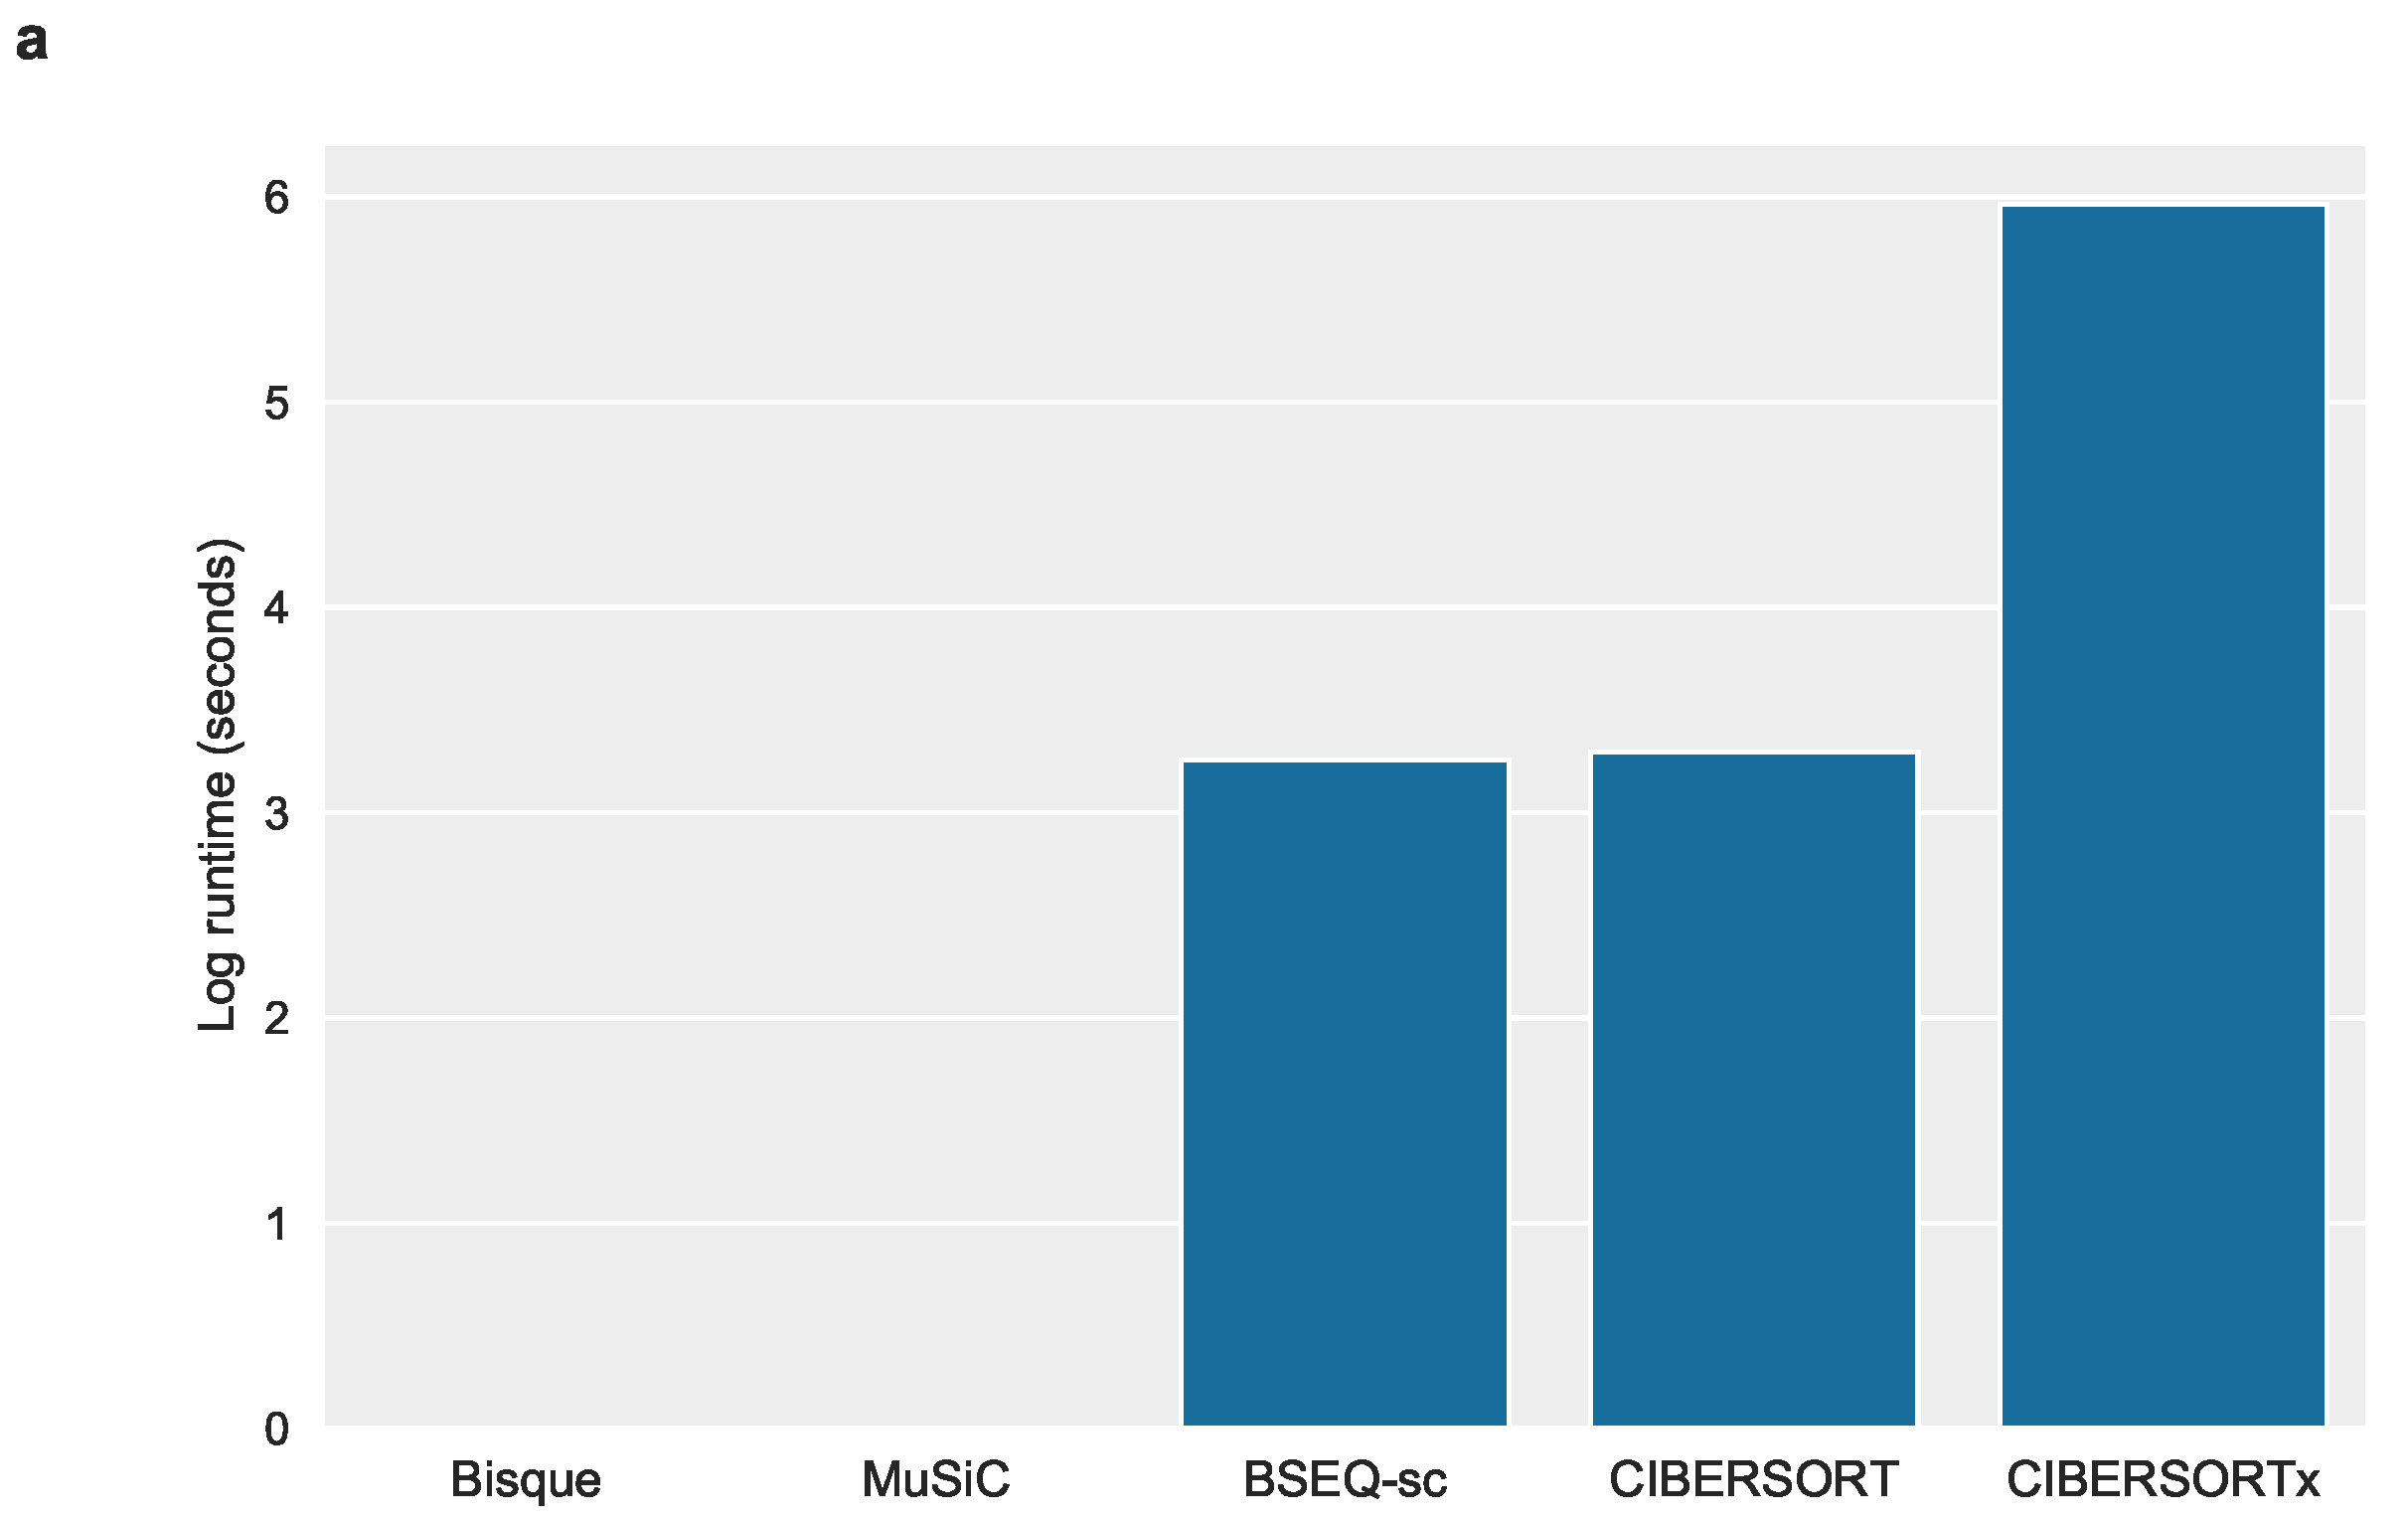
\includegraphics[scale=.19]{chapter2/figures/fig5a.pdf}
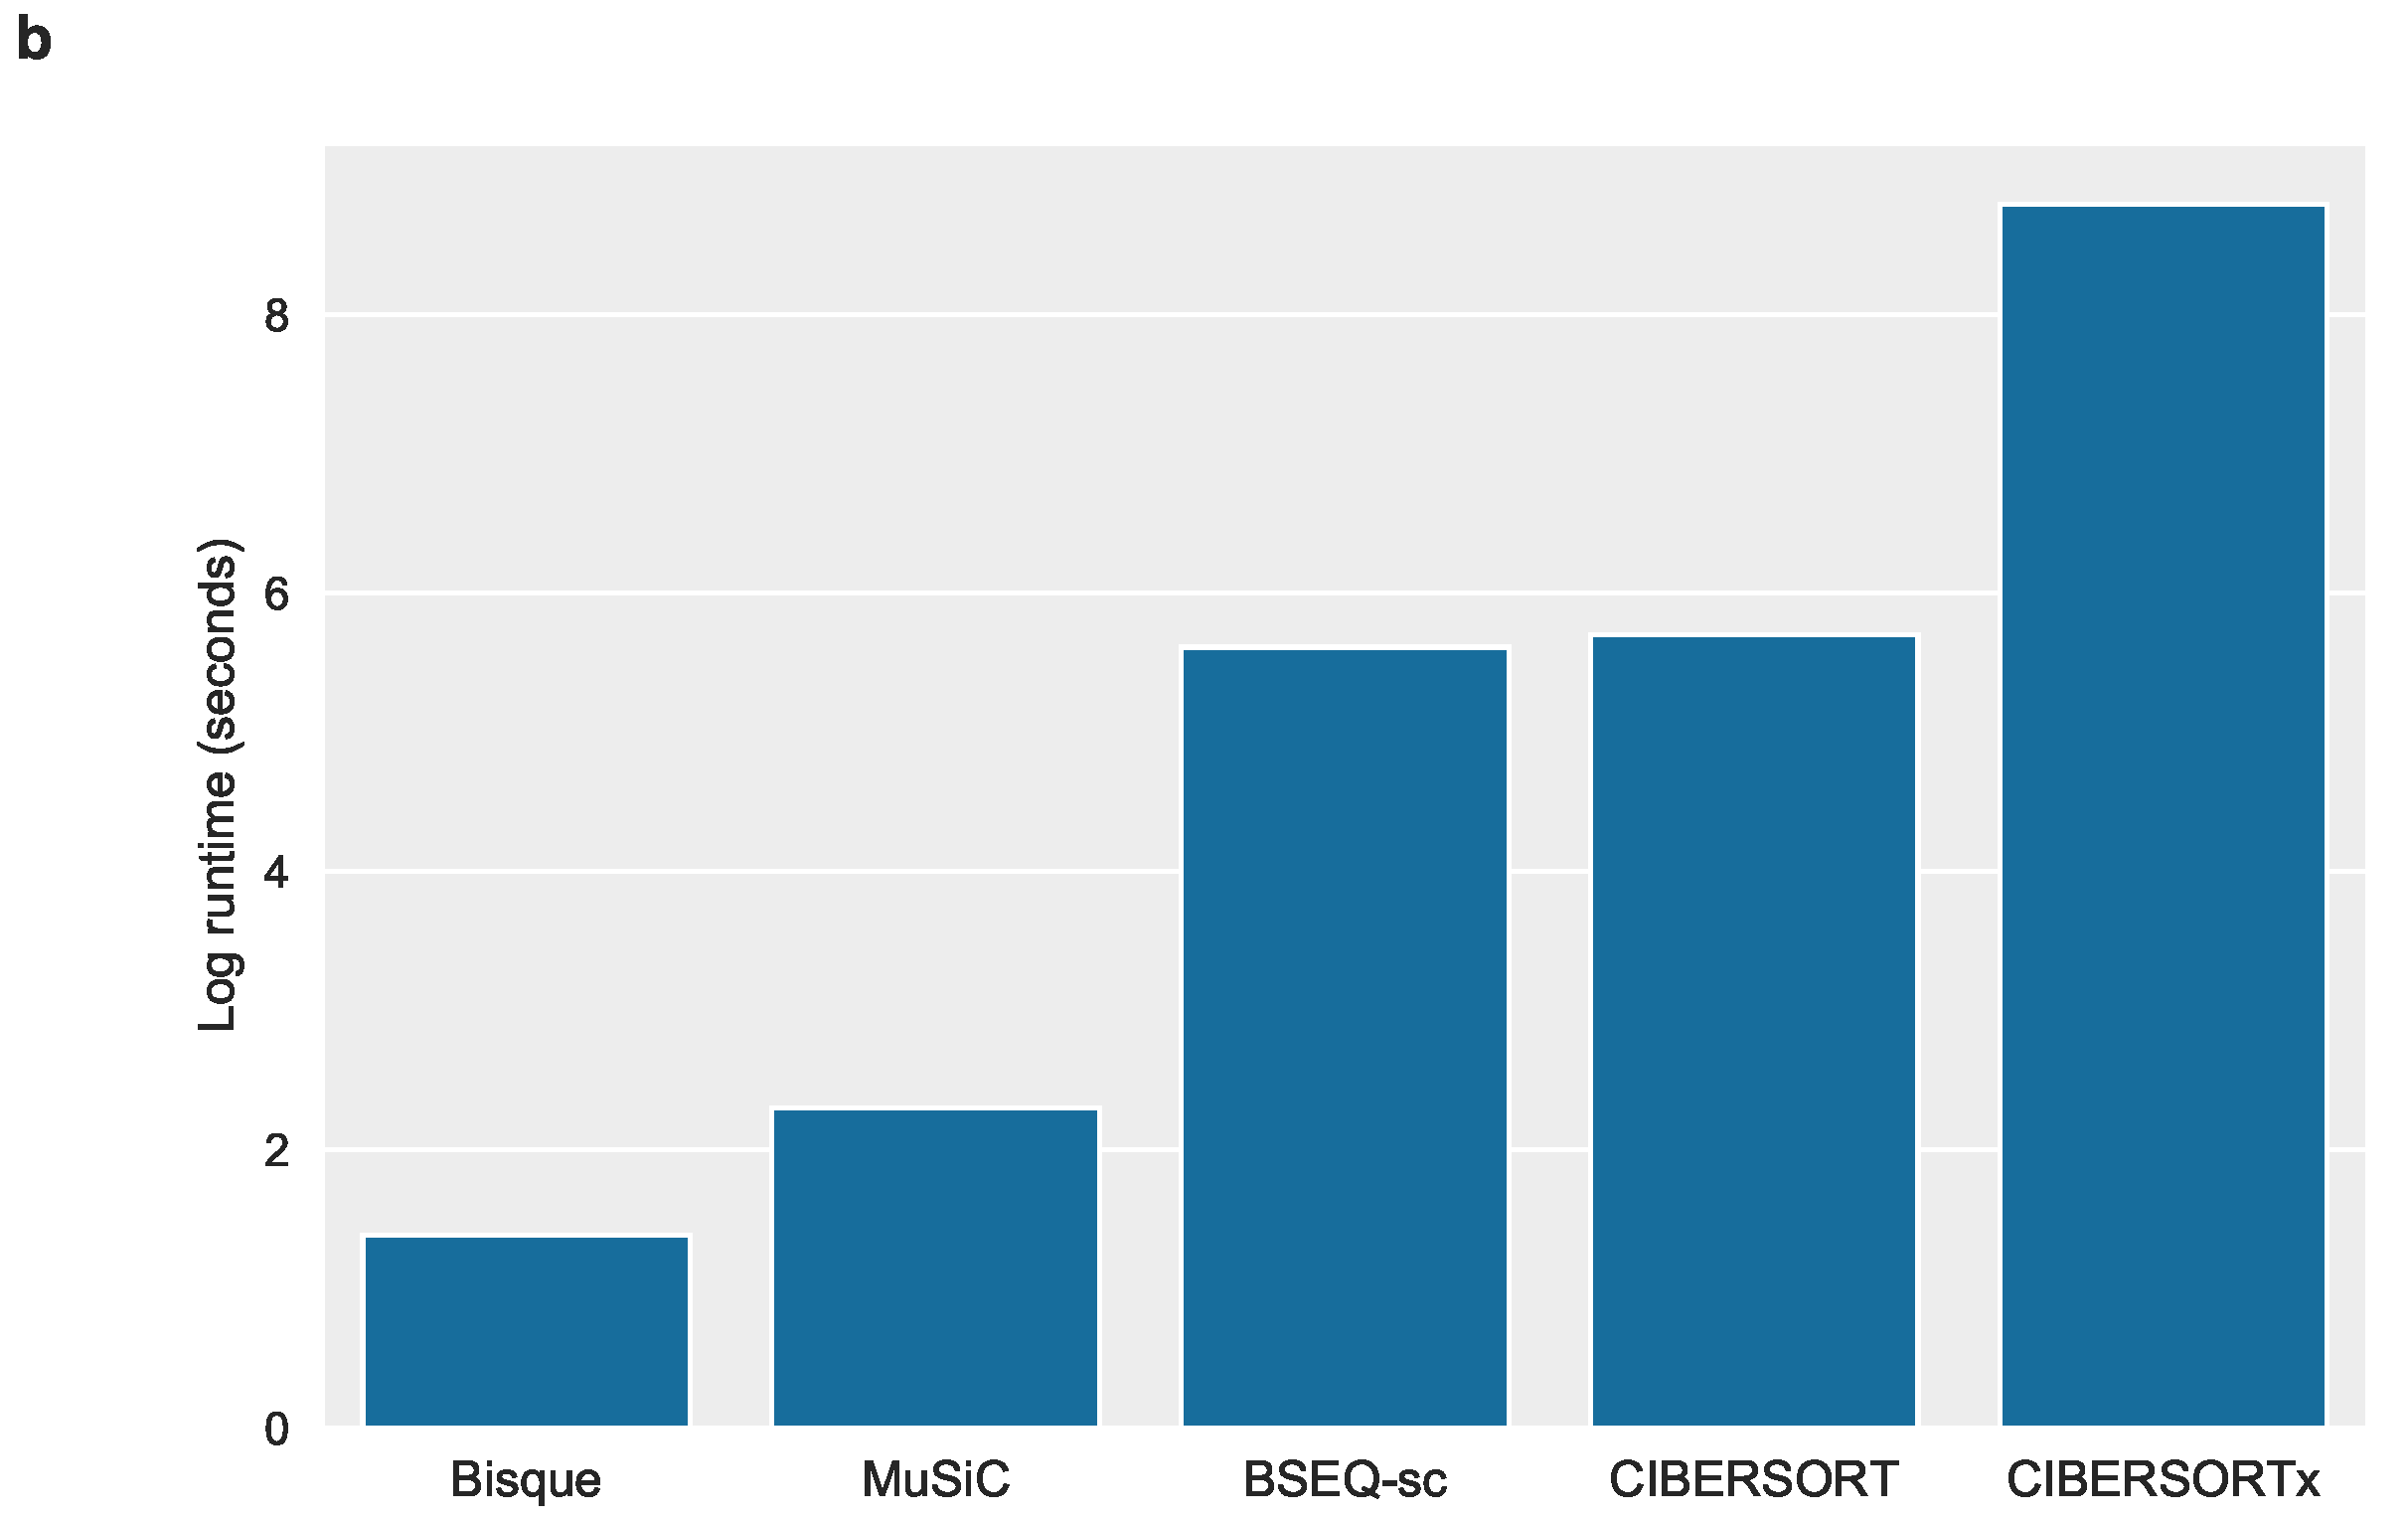
\includegraphics[scale=.19]{chapter2/figures/fig5b.pdf}
\caption{
    Runtime comparisons in log-transformed seconds for benchmarked reference-based decomposition methods.
    (\textbf{a}) Runtime for subcutaneous adipose dataset, which included 100 RNA-seq samples and 6 snRNA-seq samples with around 1,800 nuclei per individual.
    (\textbf{b}) Runtime for dorsolateral prefrontal cortex dataset, which included 628 RNA-seq samples and 8 snRNA-seq samples. We benchmarked each method using around 2,125 nuclei per snRNA-seq sample.
    }
\label{fig:fig2.5}
\end{figure}


\subsection{Robustness of the reference-based decomposition model}

Our reference-based decomposition method is based on the assumption that cell populations are equally represented in single-cell and bulk RNA sequencing of the same tissue samples. Since this assumption may be violated~\cite{Schelker2017-ms}, we explored the performance of our model as we relaxed this assumption in simulations. First, we simulated snRNA-seq data where cell proportions were increasingly biased. Using the DLPFC snRNA-seq data, we downsampled or upsampled the cells identified as microglia at varying levels and performed decomposition. Indeed, the absolute estimates produced by Bisque propagated these shifts in snRNA-seq proportions. However, we found that our estimates maintained their expected positive association with Braak stage, evidence for the correlation between these estimates and the true microglia proportions (Figure \ref{fig:supfig5}a).  Given these results, we suggest that users take note of this behavior if both the mean abundances are important for downstream analysis and the single-cell reference data is known to be significantly biased against specific cell populations of interest.
 
Next, we simulated a situation where an unknown cell population contributes to bulk expression but is not represented in the snRNA-seq reference data. For situations where this unknown contribution varies across the bulk dataset, we simulated bulk expression by mixing the observed bulk expression for the DLPFC dataset with increasing amounts of expression observed in the adipose dataset. To determine the effect of unknown cell populations on our model, we analyzed the distribution of residual norms produced by the method. These residual norms provide a measure of the difference between the vector of observed bulk and expression reference weighted by the estimated proportions across all genes for each individual. As we increased the contribution from unknown cell types, the residual norm values tend to increase (Figure \ref{fig:supfig5}b). In our simulation framework, this variability in unknown cell type contribution could be qualitatively identified by the presence of a multimodal residual norm distribution. 

Given that single-cell datasets still remain relatively small compared to bulk datasets, we also explored the impact of sample size in the reference single-cell data on the performance of Bisque. In the DLPFC dataset, we saw a drop in performance when using less than four randomly selected snRNA-seq samples (Figure \ref{fig:supfig5}c). This threshold is likely to differ between experiments, though we recommend at least three single-cell samples to generate reference data. 

Finally, since marker gene selection can vary between studies, we were interested in the performance of Bisque as we varied the number of marker genes. Again, we measured cell type proportion estimation performance for microglia in the DLPFC dataset by correlating the estimates with Braak stage, which is known to have a positive association. We recalculated this correlation as we removed marker genes for this cell type. We removed marker genes in order of both decreasing and increasing log-fold-change, which provides a measure of the importance of marker genes for identifying this cell type. In both procedures, we observe that as we remove an increasing percentage of the 102 identified marker genes, performance remains stable until a shared drop off point around 75\% (Figure \ref{fig:supfig5}d). Since we observed this trend in both marker gene removal schemes, we assume that a relatively few number of marker genes, regardless of their log-fold-change magnitude, can be used to accurately estimate cell type proportions. These results suggest that as long as a core set of marker genes are present, variations in less important marker genes will have little effect on downstream analyses.

\begin{figure}
\centering
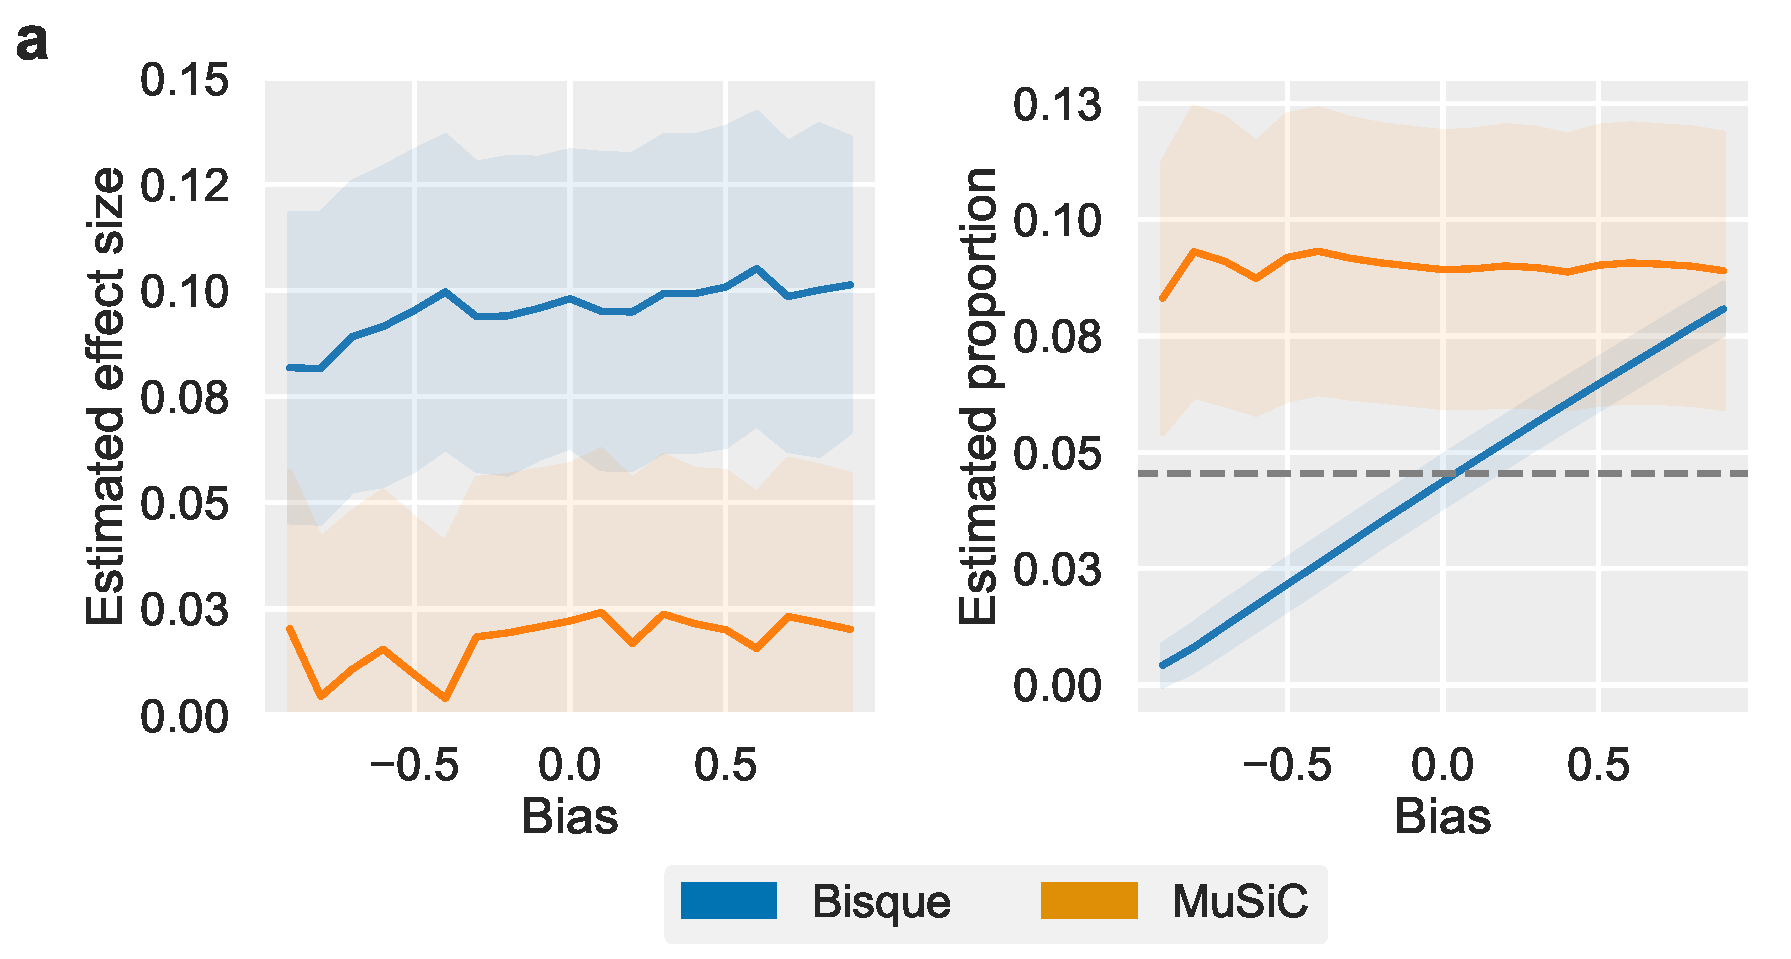
\includegraphics[scale=\figscale]{chapter2/figures/supp_fig_5ab.pdf} 
\hspace*{1cm}
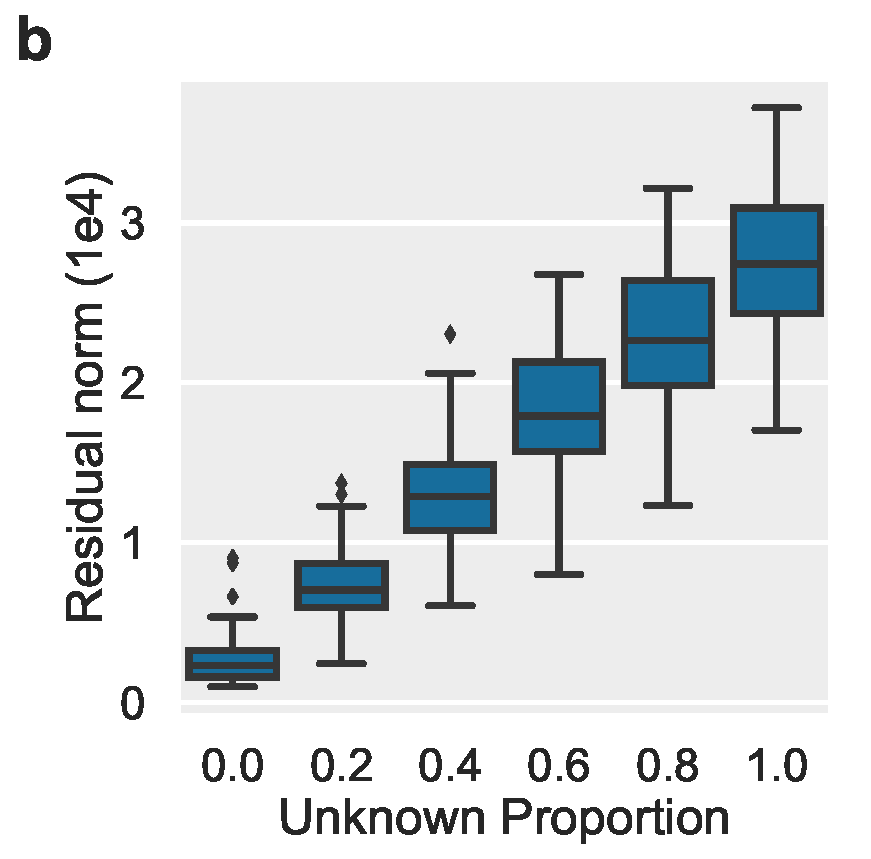
\includegraphics[scale=\figscale]{chapter2/figures/supp_fig_5c.pdf} 
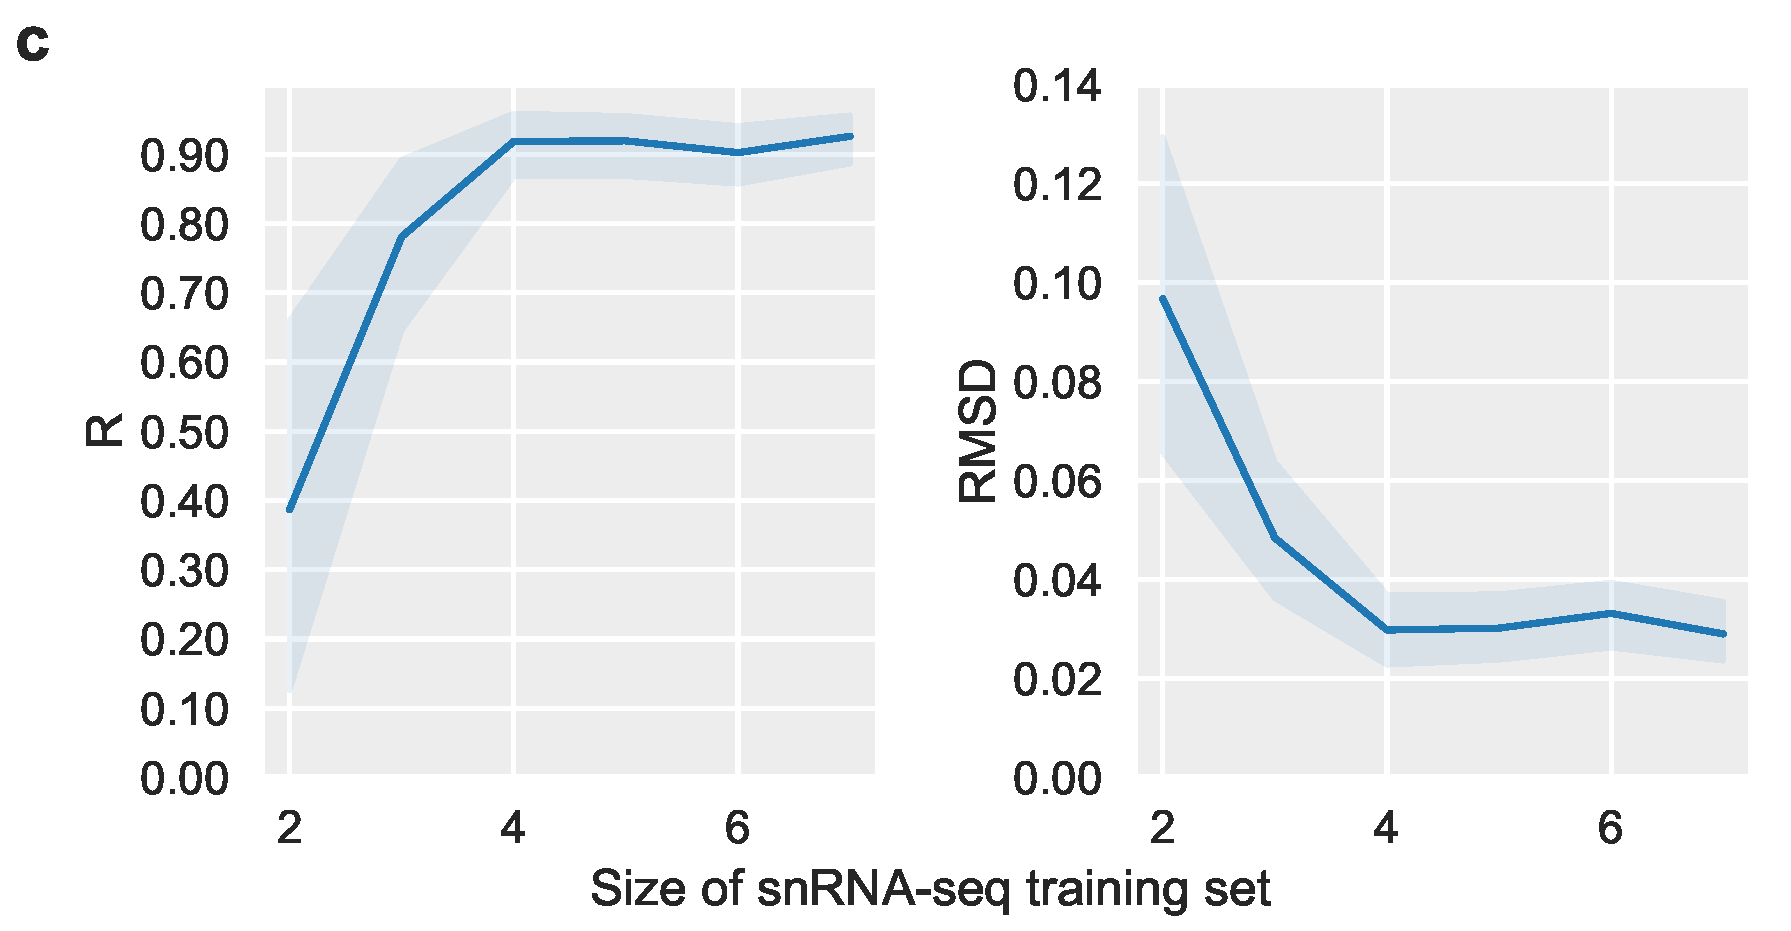
\includegraphics[scale=0.27]{chapter2/figures/supp_fig_5d.pdf}
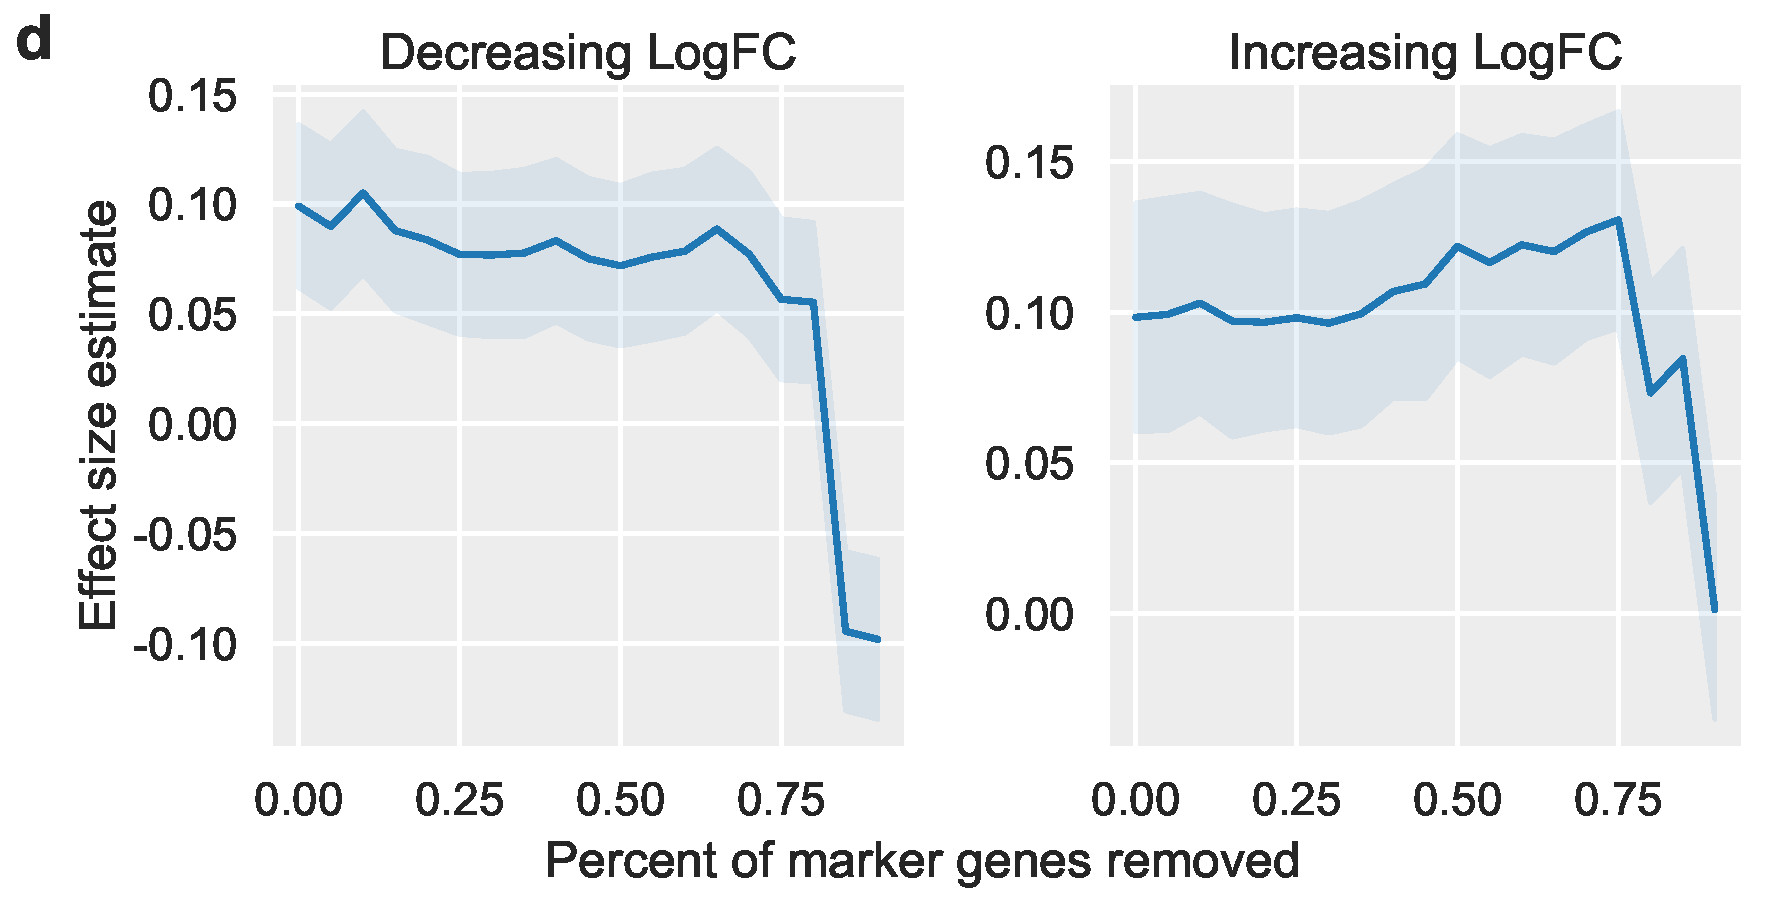
\includegraphics[scale=0.27]{chapter2/figures/supp_fig_5e.pdf}
\caption{
        Robustness of the reference-based decomposition model. 
        (\textbf{a}) Microglia cells in the DLPFC snRNA-seq data were upsampled or downsampled at various percentages, denoted as bias on the x-axis. Decomposition performance, measured as the estimated effect size of microglia proportion on Braak stage (which is expected to be positive) on the y-axis was consistent for each method as the bias in the snRNA-seq reference varied (left). The simulated bias propagates to the estimated proportions for Bisque(right). Shaded regions indicate standard error of estimates.  
        (\textbf{b}) In order to model the severity of the sample discordance due to unknown cell fractions, we compared the amount of adipose contamination, denoted as unknown proportion on the x-axis, to the residuals from the Bisque model (y-axis).
        (\textbf{c}) Leave-one-out cross-validation performance in the DLPFC dataset after utilizing random subsamples of the snRNA-seq data as a reference. Performance measured in terms of Pearson correlation (left) and RMSD (right). Shaded regions indicate 95\% confidence interval.
        (\textbf{d}) At each amount of marker genes removed (x-axis), performance was measured as the effect size of the estimated microglia proportion on Braak stage (y-axis). Genes were removed in order of decreasing (left) or increasing (right) log-fold-change. Shaded regions indicate standard error of estimates.
        }
\label{fig:supfig5}
\end{figure}

\subsection{Marker-based decomposition using known cell type marker genes }

While a reference profile from snRNA-seq can help to decompose bulk level gene expression, it may not be available for the same data set. The majority of bulk RNA-seq data sets do not have corresponding snRNA-seq data in the same set of individuals. However, marker gene information from prior experiments can still be applied to distinct expression data sets of the same tissue. The basis of most decomposition methods relies on the logic that as the proportion of a cell type varies across individuals, the expression of its marker genes will tend to correlate in the same direction as its cell type proportion. This linear co-variation can be captured in a principal components analysis (PCA). Under the same argument, the more cell type-specific a marker gene is, the more its expression will reflect its cell type proportion. These observations form the basis for BisqueMarker, a weighted PCA-based (wPCA) decomposition approach. Genes that are more specifically expressed within a cell type will provide more information than genes with shared expression across cell types. To estimate cell type proportions without the use of cell type-specific gene expression information, we applied wPCA to bulk-level adipose tissue expression.

For each cell type, we extracted the first PC from a wPCA of the expression matrix of its markers. The expression matrix was corrected for the first global expression PC as a covariate so that wPCA estimates would not reflect technical variation. We first confirmed that these genes were distinct across cell types. If 2 cell types share a high proportion of marker genes, the wPCA estimates from bulk RNA-seq will correlate highly. We then investigated whether the second or third PC could have represented cell type proportions. The percent of variance explained by the first PC was typically 30-60\% across adipose cell types, and additionally, over 90\% of the markers correlated in the same direction as the first PC. In contrast, roughly 50-70\% of markers correlated in the same direction as the second or third PC. As performed for reference-based decomposition, we correlated phenotypes with cell type proportions estimated by BisqueMarker. We identified the same associations as with reference-based decomposition, demonstrating its validity when a reference is not available (Tables \ref{table:suptable2.1a}, \ref{table:suptable2.1b}, \ref{table:suptable2.1c}). Similarly, we observed the same trends between estimated cell type abundances and phenotypes as we did using our reference-based method in the DLPFC cohort (Tables \ref{table:suptable2.2a}, \ref{table:suptable2.2b}). 

\section{Discussion}

Bisque effectively leverages single-cell information to decompose bulk expression samples, outperforming existing methods in datasets with snRNA-seq data available. In simulations, we demonstrated that the decomposition accuracy of Bisque is robust to increasing variation between the generation of the reference profile and bulk expression, which is a significant issue when comparing snRNA-seq and bulk RNA-seq data. In observed bulk expression, our reference-based method accurately estimates cell proportions that are consistent with previously reported distributions and reliably detects rare cell types. We found that these estimates consistently follow expected trends with measured phenotypes, suggesting that cell-specific estimates of proportion are sufficiently accurate to extract relevant biological signals. In addition, differences in tissue structure can lead to significant differences in the quality of single-cell expression data~\cite{Nguyen2018-gv}. We demonstrated the improved performance of our method in adipose and DLPFC, two distinct tissues, suggesting that Bisque is robust across different tissue types.

The cell type proportion estimates determined by Bisque may be utilized to effectively identify cell-type-specific interactions, such as expression quantitative trait loci (eQTLs), and adjust for confounding effects from variability in cell populations. With this reference-based approach, single-cell sequencing of a subset of samples from large-scale bulk expression cohorts can provide high power to detect cell-specific associations in complex phenotypes and diseases. 

However, we note that there are limitations to this reference-based method that users should consider. First, if the number of individuals with single-cell data available is small, the reference profile and gene-specific transformations may become unreliable. In addition, a key assumption of our transformation framework is that single-cell based estimates of cell proportions accurately reflect the true proportions we wish to estimate. As a result of this assumption, Bisque provides estimates of cell proportions reported by the single-cell technology used to generate the reference data. Given that snRNA-seq can provide less bias in isolating specific cell types compared to scRNA-seq~\cite{Wu2019-pq,Bakken2018-nt}, we expect these estimates to be useful for downstream analyses such as those previously discussed. Nevertheless, the accuracy of Bisque may decrease if the proportion of cell types captured by single-cell experiments differs significantly from the true physiological distributions. Therefore, we advise users to take caution if there is a known significant bias in the single-cell measurements of a tissue, such as severe underrepresentation of a cell type of interest, that can affect downstream analysis. Our results demonstrate that even with these limitations, Bisque can be used to provide cell-type specific biological insight in relevant datasets.

In cases where these described issues may be significant, BisqueMarker provides cell type abundance estimations using only known marker genes. While this reference-free method may be less accurate than reference-based methods, it does not depend on single-cell based estimates of cell proportions or expression profiles, but rather on the fact that the expression in certain genes differs across different cell types; moreover, this method also does not model explicitly the expression level, and it is thus robust to biases in the single cell sequencing protocol. We found that BisqueMarker estimates followed expected trends with measured phenotypes; however, it should be noted that this method estimates relative differences in abundances that cannot be compared across cell types. Also, given the semi-supervised nature of this method, these cell type abundance estimates may include signals from technical or other biological variation in the data. Therefore, we highly suggest applying this method to data that is properly normalized with sources of undesired variation removed. Bisque is available as an R package on CRAN (BisqueRNA) and at \url{https://github.com/cozygene/bisque}.


\chapter{An efficient linear mixed model framework for meta-analytic association studies across multiple contexts}

\section{Background}

    Over the last decade, the scale of genomic datasets has steadily increased. These datasets have grown to the size of hundreds of thousands of individuals \cite{Bycroft2018} with millions soon to come \cite{allofus}. Similarly, datasets for transcriptomics and epigenomics are growing to thousands of samples \cite{gtex, GTEx_Consortium2020-xx, ewas}. These studies provide valuable insight into the relationship between our genome and complex phenotypes \cite{gwas}. 
    
    Identifying these associations requires statistical models that can account for biases in study design that can negatively influence results through false positives or decreased power. Linear mixed models (LMMs) have been a popular choice for controlling these biases in genomic studies, utilizing variance components to account for issues such as population stratification \cite{Kang}. These models can also be used to analyze studies with repeated measurements from individuals, such as replicates or measurements across different contexts. Meta-Tissue  \cite{Sul} is a method that applies this model in the context of identifying expression quantitative trait loci (eQTLs) across multiple tissues. In this framework, gene expression is measured in several tissues from the same individuals and the LMM is utilized to test the association between these values and genotypes. A meta-analytic approach is used to combined effects across multiple tissues to increase the power of detecting eQTLs. This approach has also been applied to increase power in genome-wide association studies (GWAS) by testing the association between genotypes and multiple related phenotypes \cite{Joo}. 
    
    However, these approaches are computationally intensive. Existing approaches for fitting these models are cubic in time complexity with respect to the number of samples across all contexts \cite{Kang, Zhou}. Here, we present an ultra-fast LMM framework specifically for multiple-context studies. Our method, mcLMM, is linear in complexity with respect to the number of individuals and allows for statistical tests in a manner of hours rather than days or years with existing approaches. To illustrate the computational efficiency of mcLMM, we compare the runtime and memory usage of our method with EMMA and GEMMA \cite{Kang, Zhou}, two popular approaches for fitting these models. We further apply mcLMM to identify a large number of eQTLs in the Genotype-Tissue Expression (GTEx) dataset \cite{GTEx_Consortium2020-xx} and compare our results from METASOFT \cite{Metasoft}, which performs the meta-analysis of the mcLMM output, to a recent meta-analytic approach known as mash \cite{Urbut2019}. Finally, to demonstrate the practicality of mcLMM on modern datasets, we perform a multiple-phenotype GWAS combining over a million observations sampled from hundreds of thousands of individuals in the UK Biobank \cite{Bycroft2018} within hours.

\section{Methods}

   \subsection{Linear Mixed Model}
        For multi-context experiments with $n$ individuals, $t$ contexts, and $c$ covariates, we fit the following linear mixed model
        
        \begin{equation}
            \mathbf{y} = X\beta + \mathbf{u} + \mathbf{e}
        \end{equation}
        
        \noindent where $\mathbf{u} \sim N(0,\sigma_g^2 K)$, $\mathbf{e} \sim N(0,\sigma_e^2 I)$,  $\mathbf{y} \in R^{nt}$ is a vectorized representation of the responses, $X \in R^{nt \times tc}$ is the matrix of covariates,
        $\beta \in R^{tc}$ is the vector of estimated coefficients, $K \in R^{nt \times nt}$ is a binary matrix where $K_{i,j} = 1$ 
        indicates that sample $i$ and sample $j$ in $Y$ come from the same individual, and $I \in R^{nt \times nt}$ is an identity matrix.
        $X$ is structured such that both an intercept and the covariate effects are fit within each context. For sake of simplicity, dimensions
        of $nt$ assume that there is no missing data; however, this is not a requirement for the model.
        
        The full and restricted log-likelihood functions for this model are
        \begin{equation}
            l_F(\mathbf{y}; \beta, \sigma_g, \delta) = \frac{1}{2}\left[-N\log{(2\pi\sigma^2_g)} - \log(|H|) - \frac{1}{\sigma^2_g}(\mathbf{y}-X\beta)^T H^{-1} (\mathbf{y}-X\beta)\right]
        \end{equation}
        \begin{equation}
            l_R(\mathbf{y}; \beta, \sigma_g, \delta) = l_F(\mathbf{y}; \beta, \sigma_g, \sigma_e) + \frac{1}{2}\left[tc\log(2\pi\sigma^2_g) + \log{(|X^TX|)} - \log{(|X^TH^{-1}X|)}\right]
        \end{equation}
        where $N$ is the total number of measurements made across the individuals and contexts, $\delta = \frac{\sigma^2_e}{\sigma^2_g}$, and $H = K + \delta I$  \cite{Welham}. These likelihood functions are maximized with the generalized least squares estimator $\hat{\beta} = (X^TH^{-1}X)^{-1}X^TH^{-1}\mathbf{y}$ and $\hat{\sigma^2_g} = \frac{R}{N}$ in the full log-likelihood and $\hat{\sigma^2_g} = \frac{R}{N-tc}$ in the restricted log-likelihood, where $R = (\mathbf{y}-X\hat{\beta})^TH^{-1}(\mathbf{y}-X\hat{\beta})$.  Our goal is to maximize these likelihood functions to estimate the optimal $\hat{\delta}$.
    
    \subsection{Likelihood refactoring in the general case}
        The EMMA algorithm optimizes these likelihoods for $\delta$ by refactoring them in terms of constants calculated from eigendecompositions of $H$ and $SHS$, where $S = I - X(X^TX)^{-1}X^T$, that allow linear complexity optimization iterations with respect to the number of individuals  \cite{Kang}. The GEMMA algorithm further increases efficiency by replacing the $SHS$ eigendecomposition with a matrix-vector multiplication \cite{Zhou}. Both approaches require the eigendecomposition of at least 1 $N$ by $N$ matrix which is typically cubic in complexity. Here, we show that our specific definition of $K$ as a binary indicator matrix allows us to refactor these likelihood functions without any eigendecomposition steps. It should be noted that EMMA and GEMMA can fit this model for any positive semidefinite K, while mcLMM is restricted to the definition described above. 
        
        First, note that $H = K + \delta I$ is a block diagonal matrix (as exemplified in Equation 5). Specifically, each block corresponds to an individual $i$ with $t_i$ contexts measured and is equal to $[\mathbf{1}_{t_i} + \delta I_{t_i}] \in R^{t_i \times t_i}$, where $\mathbf{1}_{t_i}$ is a $t_i$ by $t_i$ matrix composed entirely of 1. These properties of $H$ make its eigendecomposition and inverse directly known.
        
        The eigenvalues of a block diagonal matrix are equal to the union of the eigenvalues of each block. Moreover, the eigenvalues of $[\mathbf{1}_{t_i} + \delta I_{t_i}]$ are $t_i + \delta$ with multiplicity 1 and $\delta$ with multiplicity $t_i - 1$. Therefore, $H$ has eigenvalues $\delta$ with multiplicity $N-n$ and $t_i + \delta$ for each $t_i$. This provides our first refactoring
        
        \begin{equation}
            \log{(|H|)} = (N-n)\log{(\delta)} + \sum_{i=1}^n \log{(t_i + \delta)}
        \end{equation}
        
        The inverse of a block diagonal matrix can also be computed by inverting each block individually. Moreover, using the Sherman-Morrison formula \cite{ShermanMorrison}, the inverse of $[\mathbf{1}_{t_i} + \delta I_{t_i}]$ is known
        
        \begin{equation}
            (\mathbf{1}_{t_i} + \delta I_{t_i})^{-1} =  -\frac{1}{t+\delta}\mathbf{1}_{t_i} + \frac{1}{\delta} I_{t_i}
        \end{equation}
        
        \noindent Given each entry of $H^{-1}$, we can show algebraically that
        
        \begin{equation}
            X^T H^{-1} X = \frac{1}{\delta}(E - D)
        \end{equation}
        \begin{equation}
            E_{i,j} = 
            \begin{cases} 
                \sum\limits_{\text{ind} \in f(i)} x_{\text{ind},g(i)}x_{\text{ind},g(j)}&\mbox{if } f(i) = f(j) \\
                0 & \mbox{if } f(i) \neq f(j)
            \end{cases}
        \end{equation}
        \begin{equation}
            D_{i,j} = \sum\limits_{g \in \text{groups}} \frac{1}{t_g + \delta} \sum\limits_{\text{ind} \in f(i),f(j),g}x_{\text{ind},g(i)}x_{\text{ind},g(j)}
        \end{equation}
        
        \noindent where $f(i) = i \% t$ (modulo operator) provides the context of a given 0-indexed column of X, $g(i) = i // t$ (integer division) provides the covariate of a given index. A group $g$ defines the set of individuals that share the same number of measured contexts $t_g$. The expression ``$\text{ind} \in f(i),f(j),g$" indicates the set of all individuals that have $t_g$ measured contexts that include context $i$ and $j$. 
        
        Note that with all values independent of $\delta$ pre-computed, specifically the sum of covariate interactions within the sets of individuals indicated above, $E$ is constant with respect to $\delta$ and each entry of the symmetric matrix $D$ can be calculated in linear time with respect to the number of groups, which is less than or equal to the number of contexts $t$. For a given $\delta$, we can compute $X^TH^{-1}X$ in $O(t(tc)^2)$ time complexity. Both the restricted and full log-likelihoods require the calculation of $(X^TH^{-1}X)^{-1}$. The restricted log-likelihood requires the additional calculation of $\log{(|X^TH^{-1}X|)}$. To calculate both of these terms, we perform a Cholesky decomposition of $X^TH^{-1}X = LL^*$, where $^*$ indicates the conjugate transpose. Given this decomposition, we can compute 
        
        \begin{equation}
            \log{(|X^TH^{-1}X|)} = \sum_{i=1}^{tc} L_{i,i}^2
        \end{equation}
        \begin{equation}
            (X^TH^{-1}X)^{-1} = (L^*)^{-1}L^{-1}
        \end{equation}
        
        \noindent These operations can be done in $O((tc)^3)$ time complexity. 
        
        Let $P(X)$ denote a projection matrix and $M(X) = (I-P(X))$. Note that both $P(X)$ and $M(X)$ are idempotent. The term remaining term in the likelihood functions, $R$, can be reformulated as follows
        \begin{align}
        \begin{split}
            \mathbf{y}- X\hat{\beta} & = \mathbf{y} - X(X^TH^{-1}X)^{-1}X^TH^{-1}\mathbf{y} \\
                                     & = (I - X(X^TH^{-1}X)^{-1}X^TH^{-1})\mathbf{y} \\
                                     & = (I - P(X))\mathbf{y} \\
                                     & = M(X)\mathbf{y}
        \end{split}
        \end{align}
        
        \begin{align}
        \begin{split}
            M(X)^TH^{-1} & = (I - X(X^TH^{-1}X)^{-1}X^TH^{-1})^T H^{-1} \\
                         & = (I - H^{-1}X(X^TH^{-1}X)^{-1}X^T)H^{-1} \\
                         & = H^{-1} - H^{-1}X(X^TH^{-1}X)^{-1}X^TH^{-1} \\
                         & = H^{-1}(I - X(X^TH^{-1}X)^{-1}X^TH^{-1}) \\
                         & = H^{-1}M(X)
        \end{split}
        \end{align}
    
        \begin{align}
        \begin{split}
            R & = (\mathbf{y}-X\hat{\beta})^TH^{-1}(\mathbf{y}-X\hat{\beta})    \\
              & = \mathbf{y}^TM(X)^TH^{-1}M(X)\mathbf{y} \\
              & = \mathbf{y}^TH^{-1}M(X)M(X)\mathbf{y} \\
              & = \mathbf{y}^TH^{-1}M(X)\mathbf{y} \\
              & = (\mathbf{y}^TH^{-1}\mathbf{y}) - (\mathbf{y}^TH^{-1}X(X^TH^{-1}X)^{-1}X^TH^{-1}\mathbf{y}) \\
              & = a - \mathbf{b}^T(X^TH^{-1}X)^{-1}\mathbf{b} \\
              & = a - \mathbf{b}^T(L^*)^{-1}L^{-1}\mathbf{b}
        \end{split}
        \end{align}
        The scalar $a$ and vector $\mathbf{b}$ are a function of $\delta$ and can be algebraically formulated as
        \begin{equation}
            a = \frac{1}{\delta}\left(\left(\sum_{i=1}^{N}\mathbf{y}_i^2\right) - \left(\sum\limits_{g \in \text{groups}} \frac{1}{t_g + \delta}\sum\limits_{\text{ind} \in g}(\sum\mathbf{y}_{\text{ind}})^2\right)\right)
        \end{equation}
        
        \begin{equation}
            \mathbf{b}_i = \frac{1}{\delta}\left(\left(\sum\limits_{\text{ind} \in \text{context(i)}} x_{\text{ind},g(i)}\mathbf{y}_{\text{ind},f(i)}\right) - \left(\sum\limits_{g \in \text{groups}} \frac{1}{t_g + \delta}\sum\limits_{\text{ind} \in f(i),g} x_{\text{ind},g(i)}(\sum\mathbf{y}_{\text{ind}}) \right)\right)
        \end{equation}
        where $\sum\mathbf{y}_{\text{ind}}$ indicates the sum of responses across all contexts for an individual. With values independent of $\delta$ pre-calculated, $a$ and $\mathbf{b}$ can be calculated in linear time with respect to the number of groups. 
        
        We can reformulate the entire likelihood functions as follows
        
        \begin{align}
        \begin{split}
            l_F(\mathbf{y}; \beta, \sigma_g, \delta) & = \frac{1}{2}\left[-N\log{(2\pi\sigma^2_g)} - \log(|H|) - \frac{1}{\sigma^2_g}(\mathbf{y}-X\beta)^T H^{-1} (\mathbf{y}-X\beta)\right] \\ 
                                                     & = \frac{1}{2}\left[-N\log{(2\pi\frac{R}{N})} - \log(|H|) - N\right] \\
                                                     & = \frac{1}{2}\left[-N\log{(2\pi\frac{R}{N})} - \left((N-n)\log{(\delta)} + \sum_{i=1}^n \log{(t_i + \delta)}\right) - N\right] \\
                                                     %& = \frac{1}{2}\left[-N\log{(2\pi\frac{a - \mathbf{b}^T(L^*)^{-1}L^{-1}\mathbf{b}}{N})} - \left((N-n)\log{(\delta)} +  \sum_{i=1}^n \log{(t_i + \delta)}\right) - N\right] \\
                                                     & \approx -N\log{(a - \mathbf{b}^T(L^*)^{-1}L^{-1}\mathbf{b})} - \left((N-n)\log{(\delta)} + \sum_{i=1}^n \log{(t_i + \delta)}\right) \label{lf_iter} 
        \end{split}
        \end{align}
        
        \begin{align}
        \begin{split}
            l_R(\mathbf{y}; \beta, \sigma_g, \delta) & = l_F(\mathbf{y}; \beta, \sigma_g, \sigma_e) + \frac{1}{2}\left[tc\log(2\pi\sigma^2_g) + \log{(|X^TX|)} - \log{(|X^TH^{-1}X|)}\right] \\
                                                     & \approx (tc-N)\log{(a - \mathbf{b}^T(L^*)^{-1}L^{-1}\mathbf{b})} \\
                                                     & -\left((N-n)\log{(\delta)} + \sum_{i=1}^n \log{(t_i + \delta)}\right) - \sum_{i=1}^{tc} L_{i,i}^2 \label{lr_iter} 
        \end{split}
        \end{align}
        
        Note that Equations \ref{lf_iter} and \ref{lr_iter} remove terms that are independent of $\delta$ since they are not required for finding its optimal value, indicated by the $\approx$ symbol. These likelihoods are maximized using the optimize function in R. For the full likelihood
        
        \begin{equation}
            \hat{\sigma}_g^2 = \frac{R}{\hat{\delta}N}
        \end{equation}
        
        \noindent For the restricted likelihood
        
        \begin{equation}
            \hat{\sigma}_g^2 = \frac{R}{\hat{\delta}(N-tc)}
        \end{equation}
        
        \noindent For both likelihoods
        
        \begin{equation}
            \hat{\sigma}_e^2 = \hat{\delta}\hat{\sigma}_g^2
        \end{equation}
    \subsection{Likelihood refactoring with no missing data}
    
        When there is no missing data, the likelihood functions can be further simplified. Note that in this case, $N = nt$ and all $t_i = t$. Hence,
        
        \begin{align}
        \begin{split}
            \log{(|H|)} & = (N-n)\log{(\delta)} + \sum_{i=1}^n \log{(t_i + \delta)} \\
                        & = (nt-n)log{(\delta)} + n\log{(t + \delta)}
        \end{split}
        \end{align}
        
        If the input terms $\mathbf{y}$, $X$, and $K$ are permuted resulting in samples being sorted in order of context, and the covariates in $X$ are sorted in order of context, we can decompose $H$ and $X$ into
        
        \begin{equation}
            H = (\mathbf{1}_{t} + \delta I_t) \otimes I_n 
        \end{equation}
        \begin{equation}
            X = I_t \otimes X_{\text{dense}}
        \end{equation}
        
        \noindent where $\otimes$ indicates the Kronecker product and $X_{\text{dense}} \in R^{n \times c}$ is a typical representation of the covariates for each individual without multiple contexts (i.e. samples as rows and covariates as columns). Utilizing the properties of Kronecker products, we can perform the following reformulation

        \begin{align}
        \begin{split}
            (X^TH^{-1}X)^{-1} & = ((I_t \otimes X^T_{\text{dense}})((\mathbf{1}_{t} + \delta I_t) \otimes I_n )^{-1}(I_t \otimes X_{\text{dense}}))^{-1} \\
                              & = ((\mathbf{1}_{t} + \delta I_t)^{-1} \otimes X^T_{\text{dense}}X_{\text{dense}})^{-1} \\
                              & = (\mathbf{1}_{t} + \delta I_t) \otimes (X^T_{\text{dense}}X_{\text{dense}})^{-1}
        \end{split}
        \end{align}
        
        \begin{align}
        \begin{split}
            \log{\left(|(X^TH^{-1}X)^{-1}|\right)} & = \log{(|(\mathbf{1}_{t} + \delta I_t) \otimes (X^T_{\text{dense}}X_{\text{dense}})^{-1}|)} \\
                                      & = \log{(|(\mathbf{1}_{t} + \delta I_t)|^c|(X^T_{\text{dense}}X_{\text{dense}})^{-1}|^t)} \\
                                      & = c\log{(|(\mathbf{1}_{t} + \delta I_t)|)} + t\log{(|(X^T_{\text{dense}}X_{\text{dense}})^{-1}|)} \\
                                      & = c\log{\left(\frac{1}{(t+\delta)\delta^{t-1}}\right)} + t\log{(|(X^T_{\text{dense}}X_{\text{dense}})^{-1}|)} \\
                                      & = c\left(-\log{(t+\delta)} - (t-1)\log{(\delta)}\right) + t\log{(|(X^T_{\text{dense}}X_{\text{dense}})^{-1}|)} \label{logXHX}
        \end{split}
        \end{align}
        
        \noindent Note that the remaining determinant in Equation \ref{logXHX} will not need to be calculated since it is independent of $\delta$. Next, we show that $\hat{\beta}$ is independent of $\delta$.
        
        \begin{align}
        \begin{split}
            \hat{\beta} & = (X^TH^{-1}X)^{-1}X^TH^{-1}\mathbf{y} \\
                        & = \left((\mathbf{1}_{t} + \delta I_t) \otimes (X^T_{\text{dense}}X_{\text{dense}})^{-1}\right)X^TH^{-1}\mathbf{y} \\
                        & = \left((\mathbf{1}_{t} + \delta I_t) \otimes (X^T_{\text{dense}}X_{\text{dense}})^{-1}\right)(I_t \otimes X^T_{\text{dense}})((\mathbf{1}_{t} + \delta I_t)^{-1} \otimes I_n )\mathbf{y} \\
                        & = \left((\mathbf{1}_{t} + \delta I_t) \otimes (X^T_{\text{dense}}X_{\text{dense}})^{-1}X^T_{\text{dense}}\right)((\mathbf{1}_{t} + \delta I_t)^{-1} \otimes I_n )\mathbf{y} \\
                        & = \left((\mathbf{1}_{t} + \delta I_t) (\mathbf{1}_{t} + \delta I_t)^{-1}\otimes (X^T_{\text{dense}}X_{\text{dense}})^{-1}X^T_{\text{dense}}\right)\mathbf{y} \\
                        & = \left(I_t\otimes (X^T_{\text{dense}}X_{\text{dense}})^{-1}X^T_{\text{dense}}\right)\mathbf{y}
        \end{split}
        \end{align}
        
        This form of $\hat{\beta}$ shows that the optimal coefficients are equivalent to fitting separate ordinary least squares (OLS) models for each context. We compute $\hat{\beta}$ by concatenating these OLS estimates. Given this term, we can also compute the residuals of this model $\mathbf{s} = (\mathbf{y} - X\hat{\beta})$ and reformulate $R$ as follows.
        
        \begin{align}
        \begin{split}
            R & = (\mathbf{y} - X\hat{\beta})^TH^{-1}(\mathbf{y} - X\hat{\beta}) \\
              & = \mathbf{s}^TH^{-1}\mathbf{s} \\
              & = \sum_{i=1}^{nt}\mathbf{s}_i \sum_{j=1}^{nt} \mathbf{s}_j H^{-1}_{j,i} \\
              & = \frac{1}{\delta} \left(\sum_{i=1}^{nt} \mathbf{s}_i^2 \right) + \frac{1}{\delta(t + \delta)} \left(-\sum_{i=1}^{n} \left(\sum \mathbf{s}_{\text{ind}(i)}\right)^2\right)
              %& = \frac{1}{\delta} \left(\sum_{i=1}^{nt} \mathbf{s}_i^2 \right) + \frac{1}{t + \delta} \left(-\sum_{i=1}^{nt} \mathbf{s}_i \sum \mathbf{s}_{\text{ind}(i)}\right)
        \end{split}
        \end{align}
    
        The term $ \sum \mathbf{s}_{\text{ind}(i)} $ denotes the sum of residuals for an individual across all contexts. Let $u = \sum_{i=1}^{nt} \mathbf{s}_i^2$ and $v = -\sum_{i=1}^{n} \left(\sum \mathbf{s}_{\text{ind}(i)}\right)^2$.
        \begin{equation}
            R = \frac{1}{\delta}u + \frac{1}{\delta(t + \delta)} v
        \end{equation}
        
        Now we can reformulate the log-likelihoods, omitting terms that do not depend on $\delta$.
        
        \begin{align}
        \begin{split}
            l_F(\delta) & = -nt\log{(R)} - \log(|H|) \\
                        & = -nt\log{\left(\frac{1}{\delta}u + \frac{1}{\delta(t + \delta)} v\right)} - (nt - n)\log{(\delta)} - n\log{(t+\delta)} \\
                        & = -nt\log{\left(u + \frac{1}{t+\delta} v\right)} + n \log{\left(\frac{\delta}{t+\delta}\right)}
        \end{split}
        \end{align}
        
        \begin{align}
        \begin{split}
            l_R(\delta) & = (tc-nt)\log{(R)} - \log(|H|) - \log{(|(X^TH^{-1}X)^{-1}|)} \\
                        %& = (tc-nt)\log{\left(\frac{1}{\delta}u + \frac{1}{\delta(t + \delta)} v\right)} - (nt - n)\log{(\delta)} - n\log{(t+\delta)} + c\log{(t + \delta)} + (tc-c)\log{(\delta)} \\
                        & = (tc-nt)\log{\left(u + \frac{1}{t+\delta} v\right)} + (c-n)\log{\left(\frac{t+\delta}{\delta}\right)}
        \end{split}
        \end{align}
        
        Both functions are differentiable with respect to $\delta$. Moreover, both derivatives have the same root
        
        \begin{equation}
            \hat{\delta} = \frac{-tu - v}{u+v}
        \end{equation}
    
        The scalar values $u$ and $v$ can be calculated by performing a separate OLS regression for each context, which can be completed in $O(t(nc^2 + c^3))$ time for a naive OLS implementation. Compared to the methods described above, this approach requires no iterative optimization and the estimate is optimal. Our implementation has a time complexity of $O(c^3 + nc^2 + tcn)$. 
        
    \subsection{Resource requirement simulation comparison}
        We installed EMMA v1.1.2 and manually built GEMMA from its GitHub source (genetics-statistics/GEMMA.git, commit 9c5dfbc). We edited the source code of GEMMA to prevent the automatic addition of intercept term in the design matrix (commented out lines 1946 to 1954 of src/param.cpp).
        
        Data were simulated using the mcLMM package. Sample sizes of 100, 200, 300, 400, and 500 were simulated with 50 contexts. Context sizes of 4, 8, 16, 32, and 64 were simulated with 500 samples. Data were simulated with $\sigma^2_e=0.2$ and $\sigma^2_g=0.4$ and a sampling rate of 0.5. Memory usage of each method was measured using the peakRAM R package (v 1.0.2). 
    
    \subsection{False positive rate simulation}
        We simulated gene expression levels in multiple tissues for individuals where there were no eQTLs. In other words, gene expression levels were not affected by any SNPs. We considered 10,000 genes and 100 SNPs resulting in one million gene-SNP pairs. We simulated 1,000 individuals. We also examined false positive rates with 500 and 800 individuals. We generated 49 such datasets where the number of tissues varied from 2 to 50. To simulate the genotypes for each subject, we randomly generated two haplotypes (vectors consisting of 0 and 1) assuming a minor allele frequency (MAF) of 30\%. To simulate gene expression levels from multiple tissues among the same individuals, we sampled gene expression from the following multivariate normal distribution:
        
        \begin{equation}
            \mathbf{y} \sim N(0,\sigma_g^2\mathbf{K} + \sigma_e^2\mathbf{I} )
        \end{equation}
        
        where $\mathbf{y}$ is an $N \times T$ vector representing the gene expression levels of $N$ individuals in $T$ tissues and $\mathbf{K}$ is an $NT \times NT$ matrix corresponding the correlation between the subjects across the tissues. $K_{i,j} = 1$ when $i$ and $j$ are from two tissues of the same individuals, $K_{i,j} = 0$ otherwise. Here, we let $\sigma_g = \sigma_e = 0.5$. We used a custom R function (included with the mcLMM package) to simulate data from this distribution, which is based on sampling from a smaller covariance matrix for each block of measurements from an individual.
        
        After generating the simulation datasets, we first ran mcLMM to obtain the estimated effect sizes and their standard errors, as well as the correlation matrices. The results from mcLMM were used as the input of METASOFT for meta-analysis to evaluate the significance. False positive rate was calculated as the proportion of gene-SNP pairs with p-values smaller than the significance level ($\alpha = 0.05$).
    
    \subsection{True positive simulations}
        We developed the true positive simulation framework based on a previous study describing mash \cite{Urbut2019}. We simulated effects for 20,000 gene-SNP pairs in 44 tissues, 400 of which have non-null effects (true positives) and 19,600 of which have null effects. Let $\beta_{jr}$ denote the effects of the gene-SNP pair $j$ in context/tissue $r$ and $\beta_j$ is a vector of effects across various tissues, including null effects and non-null effects. We simulated the gene expression levels for 1,000 individuals as:
            \begin{equation}
                \mathbf{y} = \beta_{jr}^T X + \mathbf{e}
            \end{equation}
        where $X$ denotes the genotypes of the individuals that were simulated as described in the false positive rate simulation. $\mathbf{e} \sim N(0,\sigma_g^2\mathbf{K} + \sigma_e^2\mathbf{I})$, which is similar to the simulation in the false positive rate simulation. For $\beta_j$, we defined two types of non-null effects and simulated them in different ways:
        \begin{itemize}
            \item Shared, structured effects: non-null effects are shared in all tissues and the sharing is structured. The non-null effects are similar in effect sizes and directions (up-regulation or down-regulation) across all tissues, and this similarity would be stronger among some subsets of tissues. For 19,600 null effects, we set $\beta_j=0$. For 400 non-null effects, we assumed that each $\beta_j$ independently followed a multivariate normal distribution with mean 0 and variance $\omega U_k$,
            where $k$ is an index number randomly sample from ${1,\ldots,8}$. $\omega = |\omega^\prime|, \omega^\prime \sim N(0, 1)$ represents a scaling factor to help capture the full range of effects. $U_k$ are $44 \times 44$ data-driven covariance matrices learned from the GTEx dataset, which are provided in \cite{Urbut2019}.
            \item Shared, unstructured effects: non-null effects are shared in all tissues but the sharing is unstructured or independent across different tissues. For 19,600 null effects, we set $\beta_j=0$. For 400 non-null effects, we sampled $\beta_j$ from a multivariate normal distribution with mean of 0 and variance of $0.01I$, where $I$ is a $44 \times 44$ identity matrix.
        \end{itemize}
        
        After simulating the gene expression levels $\mathbf{y}$, we first ran mcLMM on the simulated datasets to acquire the estimated effect sizes and their standard errors, as well as the correlation matrices. Then we apply METASOFT for meta-analysis with mcLMM outputs to evaluate the significance. For mash, we first performed simple linear regression to get the estimates of the effects and their standard errors in each tissue separately. Later, these estimates and standard errors were used as the inputs for mash, which returned the measure of significance for each effect, the local false sign rate (lfsr). Finally, we employed the ``pROC'' R package \cite{Robin2011-ww} to calculate the receiver operating characteristic (ROC) curve and area under the ROC curve with the significance measures (p-values for mcLMM and METASOFT, lfsr for mash) and the correct labels of null effects and non-null effects.
    
    \subsection{Analysis of the GTEx dataset}
        The Genotype-Tissue Expression (GTEx) v8 dataset \cite{GTEx_Consortium2020-xx} was used in this study. We downloaded the gene expression data, the summary statistics of single-tissue cis-eQTL data, using a 1 MB window around each gene, and the covariates in the eQTL analysis from GTEx portal (https://gtexportal.org/home/datasets). The subject-level genotypes data was acquired from dbGaP accession number phs000424.v8.p2. The GTEx v8 dataset includes 49 tissues from 838 donors. And we selected 15,627 genes that express in all 49 tissues. We only included SNPs with minor allele frequency (MAF) larger than 1\% and missing rate lower than 5\%. We applied mash and mcLMM plus METASOFT to the GTEx v8 dataset in our analysis. 
        
        As mash needed to learn correlation structure among non-significant tests and data-driven covariance matrices before fitting its model. We prepared its input by selecting the top SNP with the smallest p-value and 49 random SNPs (or all other SNPs if there are fewer than 49 SNPs left in a gene) in every gene from the eQTL analysis in the GTEx v8 dataset. There were 560,475 gene-SNP pairs in total. mash used the estimated effect sizes and standard errors of these gene-SNP pairs to learn the correlation structure of different conditions/tissues and later the canonical covariances. And we used the top SNPs to set up the data-driven covariances. Then we fitted mash to the random set of gene-SNP pairs with the canonical and data-driven covariances. With the fitted mash mode, we computed the posterior summaries including local false sign rate (lfsr) \cite{stephens2017false} for the selected gene-SNP pairs to estimate the significance. We defined significant gene-SNP pairs as those with lfsr $<$ 0.05 in any tissues. 
        
        We applied mcLMM to the same set of gene-SNP pairs. We regressed out unwanted confounding factors in gene expression levels for each tissue with a linear model using covariates provided by GTEx. Covariates of each sample included 
        top 5 genotyping principal components, PEER factors \cite{Stegle2012-zc} (15 factors for tissues with fewer than 150 samples, 30 factors for those with 150-250 samples, 45 factors for those with 250-350 samples, and 60 factors for those with more than 350 samples), sequencing platform, and sex. Then we ran mcLMM with the SNP genotypes and processed gene expression levels of all 838 individuals across 49 GTEx tissues for each gene-SNP pair. Missing values in gene expression were allowed. The effect sizes, standard errors, and correlation matrices estimated by mcLMM were meta-analyzed with METASOFT to evaluate the significance. A gene-SNP pair was significant if its p-value was smaller than 0.05. We considered both FE and RE2 models of METASOFT in the calculation of p-values.
    
    \subsection{Analysis of the UK Biobank dataset}
        This work was conducted using the UK Biobank Resource under application 33127. Samples were filtered for Caucasian individuals (Data-Field 22006)). Hard imputed genotype data from the UK Biobank were LD pruned using a window size of 50, step size of 1, and correlation threshold of 0.2. SNPs were further filtered for minor allele frequency of at least 0.01 and a Hardy-Weinberg equilibrium p-value greater than 1e-7 using Plink 2 \cite{PLINK2}. Samples were filtered for unrelated individuals with KING using a cutoff value of 0.125 \cite{KING}. Genotype data were split by chromosome and converted to bigsnpr format (v 1.4.4) for memory efficiency \cite{bigsnpr}.
        
        The following data fields were retrieved: age at recruitment (Data-Field 31), sex (Data-Field 21022), BMI (Data-Field 23104), body fat percentage (Data-Field 23099), 10 genetic principal components (Data-Field 22009), HDL Cholesterol (Data-Field 30760), LDL Direct (Data-Field 30780), Apolipoprotein A (Data-Field 30630), Apolipoprotein B (Data-Field 30640), and Triglycerides (Data-Field 30870). Continuous phenotypes were visually inspected and triglycerides were log-transformed due to skewness. Data were filtered for complete observations. All fields were scaled to unit variance and centered at 0. 
        
        HDL cholesterol, LDL cholesterol, Apolipoprotein A, Apolipoprotein B, and triglycerides were combined as response variables in the LMM and age, sex, BMI, body fat percentage, and the top 10 genetic principal components were used as additional covariates in the model. Each SNP was marginally fit with mcLMM. The coefficients output by this model for each phenotype were meta-analyzed to calculate FE p-values using METASOFT as packaged with Meta Tissue v 0.5. The top GWAS hits for five different chromosomes (one per chromosome) were validated using the NHGRI-EBI GWAS catalog \cite{GWAS_catalog} and compared to studies for LDL and HDL cholesterol (GCST008035 and GCST008037).
        
\section{Results}

    \subsection{Multi-context linear mixed models}
        We implement the statistical model described in Meta-Tissue  \cite{Sul}, where we model the multi-context data as follows:
        
        \begin{equation}
            \mathbf{y} = X\beta + \mathbf{u} + \mathbf{e}
        \end{equation}
        where $\mathbf{u} \sim N(0,\sigma_g^2 K)$ and $\mathbf{e} \sim N(0,\sigma_e^2 I)$. For $n$ individuals and $t$ contexts, $\mathbf{y}$ is a vector of $nt$ responses, $K$ is an $nt$ by $nt$ binary matrix where a value of $1$ indicates that the observations were sampled from the same individual. Compared to a standard regression model, the variance component $\mathbf{u}$ accounts for within-individual variation that may occur with repeated sampling. The design matrix $X$ fits coefficients $\beta$ for each feature within each context independently. These coefficients, which describe the effect of the feature on the response within each context, can be used in a meta-analytic framework to combine the results. In our pipeline, we utilize the random effects model (RE2) from METASOFT, which assumes that effect sizes may be different across contexts and was shown to outperform existing meta-analysis methods \cite{Metasoft}.
        
        Fitting this LMM requires estimation of the parameters $\sigma^2_g$ and $\sigma^2_e$, which can be estimated with traditional likelihood or restricted-likelihood approaches or through various optimized methods that have been developed, such as EMMA and GEMMA \cite{Kang, Zhou}. These approaches require an eigendeomposition of the matrix $K$ with is traditionally considered to be an $O((nt)^3)$ operation. mcLMM utilizes the block structure of the matrices in this model to perform matrix operations within contexts and avoids any eigendecomposition operations. This approach provides massive speedups with runtime complexities that are linear with respect to sample size $n$ rather than cubic. As a note, mcLMM is not an approximation and fits identical models to these existing approaches.
    

    \subsection{mcLMM is computationally efficient}
        To demonstrate the efficiency of mcLMM compared to existing approaches, we applied our method to simulated data of varying sample sizes and number of contexts. For these simulations, we simulated a sampling rate of 0.5, which indicates that only half of all possible individual-context pairs of observations are expected to be sampled. 
        
        We first applied our method to simulations with a fixed number of 50 contexts and varied the sample size from 100 to 500. From these experiments, we observed that mcLMM requires computational time orders of magnitude less than EMMA and GEMMA. Similarly, when we fixed the number of samples at 500 and varied the context sizes from 4 to 64, we observed dramatically reduced runtimes for mcLMM.
        
        In these experiments, mcLMM also significantly reduces the memory footprint compared to EMMA and GEMMA, since we avoid creating any $nt$ by $nt$ matrices. In these simulations, existing approaches quickly grow memory requirements, with usages that grow to dozens of gigabytes for modestly sized datasets in the thousands of samples. mcLMM allows large-scale studies to be performed on relatively little computational resources (Figure \ref{fig:fig1}). 
        
        %% Figure 1 %%
        \begin{figure}
            \centering
            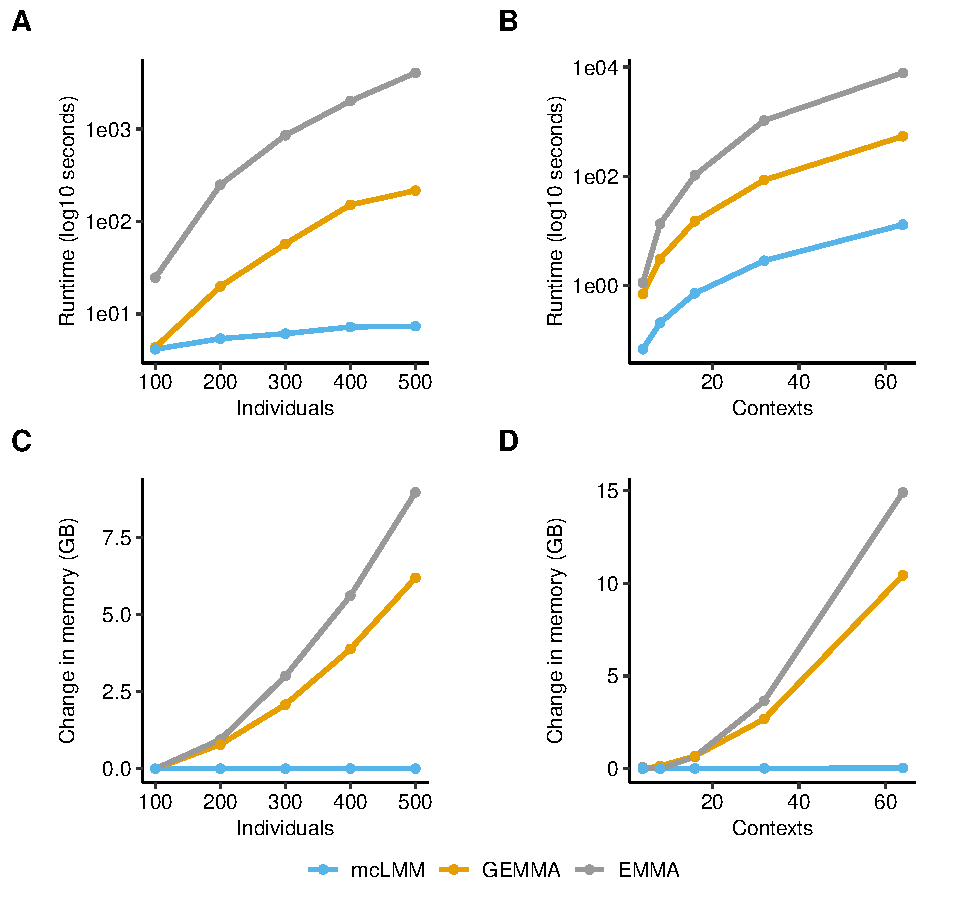
\includegraphics[width=0.75\textwidth]{chapter3/figures/Figure_1.pdf}
            \caption{Resource requirements of mcLMM, GEMMA, and EMMA across various simulated individual and context sizes with missing values (sampling rate of 0.5). For varying individuals, contexts were fixed at 50. For varying contexts, individuals were fixed at 500. (A-B) Runtime with log10(seconds) on the y-axis and number of individuals or contexts simulated on the x-axis. (C-D) Memory usage (GB) on the y-axis and number of individuals or contexts simulated on the x-axis. }
            \label{fig:fig1}
        \end{figure}
        
        In cases where there is no missing data, mcLMM allows for further speedups. We ran similar simulations to compare mcLMM with no missing data (optimal model) and mcLMM with missing data (iterative model). We observed a dramatic speedup, with sample sizes of 500,000 individuals across 10 contexts completed in under 10 seconds for the optimal model compared to around 15 minutes for the iterative model.
    
    \subsection{mcLMM enables powerful meta analyses to detect eQTLs}
        We utilized mcLMM to reduce the computational resource requirements of the Meta-Tissue pipeline, which fits a multiple-context LMM and combines the resulting effect sizes using METASOFT \cite{Sul}. While powerful, the existing approach utilizes EMMA to fit the LMM. For a recent release from the GTEx consortium  \cite{GTEx_Consortium2020-xx}, each pair of genes and single nucleotide polymorphisms (SNPs) required over two hours to run. Across hundreds of thousands of gene-SNP pairs, this method would require years of computational runtime to complete. Utilizing mcLMM, we were able to complete this analysis in 3 days parallelized over each chromosome. 
        
        We compared our approach to a method known as mash \cite{Urbut2019}. This approach utilizes effect sizes estimated within each context independently and employs a Bayesian approach to combine their results for meta-analysis. In order to estimate the power of these methods, we performed simulations as described in the methods. In null simulations, we observed well-controlled false positive rates at $\alpha = 0.05$ for mcLMM coupled with METASOFT. In our simulation with true positives, we observed an increased area under the receiver operating characteristic (AUROC) for mcLMM coupled with the random effects (RE2) METASOFT model compared to mash (Figure \ref{fig:fig2}).
        
        %% Figure 2 %%
        \begin{figure}
            \centering
            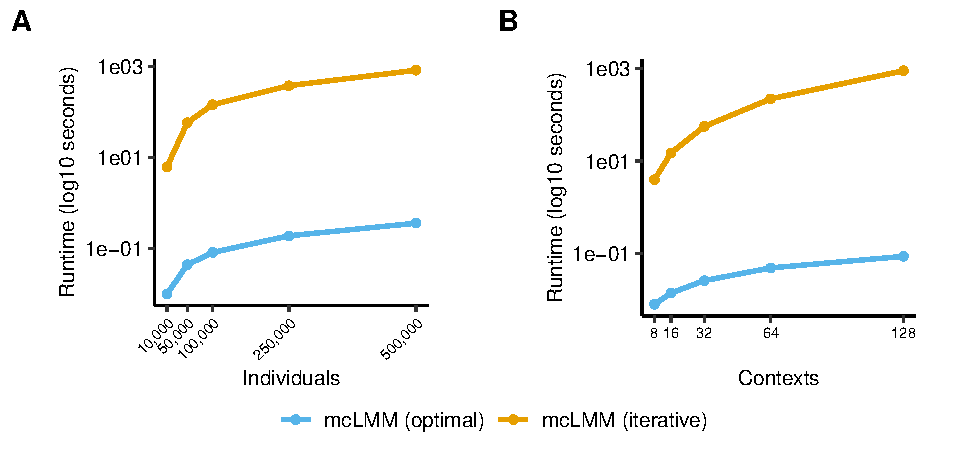
\includegraphics[width=\textwidth]{chapter3/figures/Figure_2.pdf}
            \caption{AUROC curves of mcLMM+METASOFT and mash in simulated data, assuming the effects of gene-SNP pairs are (A) shared and unstructured, and (B) shared and structured.}
            \label{fig:fig2}
        \end{figure}

        Next, we compared the number of significant associations identified in the GTEx dataset. The mash approach utilized gene-SNP effect sizes estimated by the GTEx consortium within each tissue independently. Concordant with our simulations, we observed that the Meta-Tissue approach, utilizing mcLMM for vast speedup, identified more significant eQTLs than mash (Figure \ref{fig:fig3}). These associations allow researchers to better understand the link between genetic variation and complex phenotypes through possible mediation of gene expression. 
        
        %% Figure 3 %%
        \begin{figure}
            \centering
            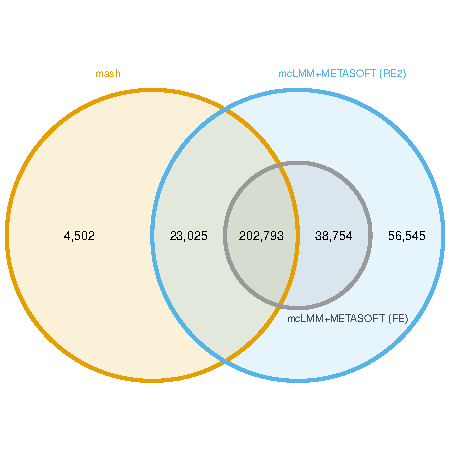
\includegraphics[width=0.75\textwidth]{chapter3/figures/Figure_3.pdf}
            \caption{Venn diagram of significant eQTLs identified by meta-analysis methods in the GTEx dataset. We compared mcLMM using two different models in METASOFT (RE2 and FE) to mash. Note that areas are not proportional to the number of eQTLs in each region. mcLMM+METASOFT (RE2) identified a total of 321,117 significant associations that contained 225,818 eQTLs identified by mash.}
            \label{fig:fig3}
        \end{figure}
        
    \subsection{mcLMM scales to millions of samples across related phenotypes}
        As a practical application of the efficiency of mcLMM, we performed a multiple phenotype GWAS in the UK Biobank. A multiple phenotype GWAS associates SNPs with several related phenotypes in order to increase the effective sample size for greater power, under the assumption that the phenotypes are significantly correlated. For our analysis, we combined HDL and LDL cholesterol, Apolipoprotein A and B, and triglyceride levels across 323,266 unrelated caucasian individuals in the UK Biobank. In total, 1,616,330 observations of these related phenotypes were fit as responses in the LMM. 
        
        The mcLMM approach completed this analysis over 211,642 SNPs with an additional 14 covariates, parallelized over each chromosome, within a day. Each chromosome was analyzed on a single core machine with 32 GB of memory, with each test taking around 2 seconds to complete. We identified several significant loci, a subset of which replicate previous findings for specific phenotypes included in the model, such as HDL cholesterol \cite{Wojcik} (Figure \ref{fig:fig4}). Existing approaches, namely EMMA and GEMMA, require orders of magnitude more memory to begin this analyses and could not be run on the available computational resources.
        
        %% Figure 4 %%
        \begin{figure}
            \centering
            \includegraphics[width=\textwidth]{chapter3/figures/Figure_4.png}
            \caption{Multiple phenotype GWAS results from UK Biobank. Five phenotypes (LDL cholesterol, HDL cholesterol, Apolipoprotein A, Apolipoprotein B, and triglyceride levels) were used as responses in the mcLMM framework. The model was fit with 1,616,330 observations from 323,266 unrelated Caucasian individuals. In total, 211,642 SNPs were tested with an additional 14 covariates. Each test required around 2 seconds to run on a 32GB machine and was parallelized over each chromosome. The -log10 of the p-values are plot on the y-axis and genomic positions on the x-axis. The horizontal dashed line indicates the genome wide significance level at $p=0.05/1e6$. The top hit for 5 different chromosomes is annotated with the gene containing the SNP. These genes have been previously identified as associated with a subset of these phenotypes.}
            \label{fig:fig4}
        \end{figure}
\section{Discussion}

    We presented mcLMM, an efficient method for fitting LMMs used for multiple context association studies. Our method provides exact results and scales linearly in time and memory with respect to sample size, while existing methods are cubic. This efficiency allows mcLMM to process millions of samples over several contexts within a day on minimal computational resources, as we showed in simulation and in the UK Biobank. The association parameters learned by mcLMM can further be utilized with the METASOFT framework to provide powerful meta-analysis of the associations, as we showed in the GTEx dataset. 
    
    Previous work has observed the potential speedup to linear complexity for LMMs when the matrix $K$ is approximated with a low rank representation \cite{Lippert2011}. Here, we optimize the method specifically for the low rank matrix that arises naturally in multiple context association studies, allowing our method to provide exact results and scale to hundreds of thousands of samples with minimal computational resources.

\chapter{Selection contributes to skewed X chromosome inactivation across human tissues}

\section{Background}
X chromosome inactivation (XCI) occurs in blastocysts during embryonic development. Under no external pressures, the process is assumed to be random and is established in about a dozen cells and all daughter cells will inherit the XCI status of these cells \cite{Takagi1975-es}. Skew in XCI has been widely observed in female mammals and is accepted to be common across individuals \cite{Shvetsova2019-re}. Selective pressures have been implicated in contributing to XCI skew, especially in the context of diseases such as cancer \cite{Brown1999-dc,Migeon1998-gc}. In addition, XCI skew was found to be heritable and correlated with age based on a twin study \cite{Zito2019-hu}. Recent work argued that observed XCI skew in the general female population is the result of expected randomness in early development \cite{Shvetsova2019-re}. 

Here, we show that XCI skew in a general female population in the GTEx dataset \cite{GTEx_Consortium2020-xx} is associated with genetic scores related to deleteriousness and proliferative potential. We hypothesize that differences in the fitness of maternal and paternal X chromosomes may contribute to skewed XCI across tissues into adulthood (Figure \ref{fig:fig4.1}a).  Furthermore, we perform a scan of common variants across the X chromosome to identify specific loci associated with overall XCI skew in these individuals.

\begin{figure}[ht]
    \centering
    \includegraphics[width=\textwidth]{chapter4/Figures/Figure_1.pdf}
    \caption{
        Measuring XCI skew across tissues 
        \textbf{a}, Schematic overview of selection hypothesis. An individual inherits one haplotype (red) that is more fit than the other (blue) due to genetic variation. Given equal population sizes in embryonic development, we hypothesize that fitness differences will produce skewed populations in fully developed tissues.
        \textbf{b}, Violin plot of absolute XCI skew on the y-axis. Tissues are sorted by mean on the x-axis. Dots indicate mean of the absolute skew with vertical lines indicating one standard deviation.}
    \label{fig:fig4.1}
\end{figure}

\section{Methods}
\subsection{Transcriptomic and genetic data}

The following data were processed and made available by the GTEx consortium \cite{GTEx_Consortium2020-xx}. GENCODE v26 and the GRCh38 human reference genome was used to process both WGS and RNA-seq data. RNA-seq data was aligned using STAR with WASP filtering. Allele-specific read counts at heterozygous sites were quantified with GATK ASEReadCounter. Genetic variants were called from whole genome sequencing data and phased with read-aware SHAPEIT2. All analyses were restricted to caucasian samples. 

\subsection{Quantifying XCI skew}

Allele-specific read counts were matched to haplotypes from the phased WGS data. Only heterozygous sites within fully inactivated genes reported by Carrel and Willard \cite{Carrel2005-zm} and Cotton et al \cite{Cotton2013-jl} were considered. Furthermore, we restricted to genes where no females were observed to escape inactivation in Cotten et al. LiftOver (https://genome.ucsc.edu/cgi-bin/hgLiftOver) was used to convert these reported gene windows from GRCh37 to GRCh38 positions. Moreover, we only considered variants that had at least 10 overlapping reads. XCI skew was calculated at each heterozygous site in the gene windows as the number of reads coming from haplotype 1 divided by the total number of reads at the site. The final XCI skew measurement for each sample was the median of these per-site observations. In addition, since haplotypes are not readily distinguishable as maternal or paternal, we also calculated the absolute XCI skew as the absolute deviation of this value from 0.5. 

We also calculated skew in the same manner in autosomes. Specifically, if $m$ heterozygous sites were used to calculate XCI in a sample, we randomly selected $m$ heterozygous sites with at least 10 overlapping RNA-seq reads on the q-arm of each non-acrocentric autosome. We used these sites to calculate skew for each autosome. 

\subsection{Genetic score association}

Four scores were defined to measure genetic burden of X chromosome haplotypes in females. First, we considered the difference in average CADD score \cite{Rentzsch2019-pk} between the two haplotypes. A higher CADD score corresponds to an increased likelihood of deleteriousness. CADD Phred scores were retrieved using VEP \cite{McLaren2016-jd}. The CADD score associated with each alternate allele on each haplotype was averaged. The remaining scores were proportions of different types of mutations carried by a haplotype. We considered the proportion of alternate alleles, missense mutations, and synonymous mutations carried by a haplotype. This proportion is calculated as the count of the variant-type on one haplotype divided by the total number of these variants found across both haplotypes. Annotations indicating the coding consequence of variants were obtained using VEP.

We associated these scores with XCI skew using a linear mixed model. Specifically, we used the lmer function from the lmerTest package \cite{Kuznetsova2017-jp} to fit the following model across all tissues, where the (1\textbar Grouping) notation indicates a random intercept for the specified grouping:
\begin{equation}
\text{H1 XCI Skew} \sim \text{H1 Burden + Age + (1\textbar Individual) + (1\textbar Tissue)}
\end{equation}
In this model, we include random intercepts for the individual and tissue of origin for each sample. The significance of these associations were determined using a one-sided t-test, under the assumption that increased burden will decrease skewing towards a haplotype.

Blood-related polygenic scores were retrieved from PGS Catalog \cite{Lambert2021-iu}. We used scores for the following cell counts: platelet (PGS000186), red blood cell (PGS000187), basophil (PGS000163), neutrophil (PGS000182), eosinophil (PGS000165), monocyte (PGS000177), and lymphocyte (PGS000172) \cite{Vuckovic2020-gf}. GRCh38 positions of the variants used for these scores were retrieved from SNP Nexus \cite{Oscanoa2020-ac}. We calculated each polygenic score for both haplotypes and modeled the difference in scores as follows:
\begin{equation}
\text{H1 XCI Skew} \sim \text{(H1 PGS - H2 PGS) + Age + (1\textbar Individual) + (1\textbar Tissue)}
\end{equation}
The significance of these associations were determined by using a one-sided t-test, under the assumption that increased proliferative potential will increase skewing towards a haplotype. 

Each of these tests were also performed for autosomes as controls with the following model:

\begin{align}
\begin{split}
\text{H1 XCI Skew} \sim & \text{ (H1 PGS - H2 PGS) + Age +} \\
                        & \text{ (1\textbar Individual) + (1\textbar Tissue) + (1\textbar Chromosome)}
\end{split}
\end{align}
where “Chromosome” refers to the autosome used to calculate skew. A Bonferroni-corrected significance threshold of 0.05/8 was used for the 4 burden scores and 0.05/14 was used for the 7 blood-related polygenic scores. 

\subsection{Identifying significant XCI loci}

The phased X chromosome variants were filtered with PLINK 2 \cite{PLINK2}. SNPs were extracted with a minor allele frequency threshold of 0.01 and Hardy-Weinberg equilibrium p-value threshold of 1e-6. LD pruning was performed with a window size of 100 kilobases, step size of 5 variants, and $r^2$ threshold of 0.5. 

These filtered variants were marginally tested in a linear mixed model to measure association with absolute XCI skew. We fit the following linear mixed model:
\begin{equation}
\text{Absolute XCI Skew} \sim \text{Heterozygous + Age + (1\textbar Individual) + (1\textbar Tissue)}
\end{equation}
where Heterozygous is 1 if the sample is heterozygous for the variant and 0 if the sample is homozygous. We modeled absolute skewing under the assumption that heterozygosity will lead to differences in fitness and consequently increased overall skewing. Given this assumption, we determined the significance of these associations using a one-sided t-test under this hypothesis. The resulting p-values were converted to q-values \cite{Storey2003-kx} and considered significant using a threshold corresponding to a 0.05 local false discovery rate.

At the two significant loci, this linear mixed model was also used to determine the significance of the difference in skewing between homozygous samples and groups defined by the phasing of the variant in heterozygous individuals. For these associations, we fit the following model separately for individuals with the variant on H1 and on H2:
\begin{equation}
\text{H1 XCI Skew} \sim \text{Heterozygous + Age + (1\textbar Individual) + (1\textbar Tissue)}
\end{equation}
Since we do not assume the direction of individual variant effects on XCI skewing, we performed a two-sided t-test to determine significance of these associations. 

\subsection{Associating XCI-linked genetics in males}

To address the possibility that the burden and proliferation scores are capturing regulatory effects, such as downregulation of a haplotype rather than increased inactivation, we calculated these scores within males. Like in the female samples, we utilized variants outside of the fully inactivated genes used to calculate skew. Given that males have one X chromosome, we associated these scores with the expression of each gene on the X chromosome. We fit a model similar to those used for identifying expression quantitative trait loci. Specifically, we performed a linear regression within each tissue independently, correcting for the top 5 genetic principal components, PCR, and platform. We also corrected for PEER factors, \cite{Stegle2012-uf} using 15 for sample sizes less than 150 and adding an additional 15 factors for each 100 samples. The resulting p-values from the linear regression were converted to q-values \cite{Storey2003-kx} and considered significant at a local false discovery rate threshold of 0.05. 

\section{Results}

\subsection{Estimating XCI skew from RNA-seq data}

We analyzed data generated by the GTEx consortium \cite{GTEx_Consortium2020-xx}, which included RNA-seq and phased whole genome sequencing data measured across 243 caucasian female samples and 472 caucasian male samples. We measured XCI skew in females as the difference in expression measured from each X chromosome in an RNA-seq experiment. Since XCI does not completely silence the entire X chromosome, we restricted our analysis to genes that have been previously observed to be fully inactivated \cite{Carrel2005-zm,Cotton2013-jl,Tukiainen2017-xm}. Read counts at heterozygous sites in these regions were assigned to haplotypes determined with phased whole genome sequencing data. The skew in RNA-seq reads was calculated at each site as the number of reads coming from one haplotype divided by the total number of reads. XCI skew for a sample was calculated as the median of these values. A median of 45 heterozygous sites were used for this calculation across the samples (Figure \ref{fig:supp_fig4.1}). We observed variability in XCI skew across tissues, with EBV-transformed lymphocytes exhibiting nearly complete skew in many samples (Figure \ref{fig:fig4.1}b).  Given this extreme skewing likely due to culture conditions, we removed these samples from downstream analyses. Furthermore, we observed correlation of XCI skew across the different tissues (Figure \ref{fig:supp_fig4.2}).

\begin{figure}[ht]
    \centering
    \includegraphics[width=0.75\textwidth]{chapter4/Figures/Supplementary_Figure_1.png}
    \caption{
        Histogram of number of heterozygous sites with coverage of 10 or more RNA-seq reads and within fully inactivated genes used to calculate XCI skew for each sample. We observed a mean of 46.805 and median of 45 variants used to calculate skew (the median of per-site skew). 
    }
    \label{fig:supp_fig4.1}
\end{figure}
\begin{figure}[ht!]
    \centering
    \includegraphics[width=0.75\textwidth]{chapter4/Figures/Supplementary_Figure_2.png}
    \caption{
        Pearson correlation of XCI skew between tissues.
        \textbf{a}, Correlation matrix of tissue-specific XCI skew. White boxes with 'X' symbol indicate that less than 25 observations were available for the tissue pair.
        \textbf{b}, Histogram of correlation between 1,017 non-identical tissue pairs. We observed a mean correlation of 0.3663 and median of 0.3992.
    }
    \label{fig:supp_fig4.2}
\end{figure}

Inferring XCI skew from expression data can be confounded by both technological and biological factors that may lead to similar associations with our genetic burden scores. Reference bias, the tendency for RNA-seq reads with reference alleles to better map to a reference genome than non-reference alleles \cite{Stevenson2013-cg}, may be a significant confounding variable. This bias is especially relevant to the genetic burden defined by the proportion of alternate alleles carried by a haplotype. For example, an alternate allele may have lower observed expression than the reference allele simply due to reference bias rather than XCI skew. To account for this source of bias, we utilized RNA-seq reads that were aligned with a filter utilizing WASP, a method that accounts for reference bias by mapping reads with swapped genotypes \cite{Van_de_Geijn2015-oy}.
Regulatory effects of genetic variation may also lead to imbalances in expression measured from each X chromosome that may be erroneously attributed to skew in X chromosome inactivation. To address this source of confounding, we performed similar experiments using the non-acrocentric autosomes (chromosomes with arms of roughly equal size) of the female samples. In short, we calculated skewing at heterozygous sites that were captured by RNA-seq reads on the q or long arm of the autosome. We observed no significant level of average ‘skewing’ in these chromosomes (Figure \ref{fig:supp_fig4.3}). 

\begin{figure}[ht]
    \centering
    \includegraphics[width=0.75\textwidth]{chapter4/Figures/Supplementary_Figure_3.png}
    \caption{
        Estimated absolute skew in expression at heterozygous sites on the X chromosome and non-acrocentric autosomes. On the X chromosome, this value is used as the estimate of inactivation skewing since heterozygous sites are within fully inactivated genes. On the autosomes, an equal number of heterozygous sites used on the X chromosome for each sample were randomly selected from the q-arm to estimate the median skew in expression. Dots indicate mean of absolute skew with vertical lines indicating one standard deviation.
    }
    \label{fig:supp_fig4.3}
\end{figure}

We also performed an analysis of the male GTEx samples to test the possibility of regulatory effects rather than skewing in inactivation. Since males only have one X chromosome, we associated genetic features with expression of each gene on the X chromosome. If our genetic scores are associated with downregulation of expression rather than cause XCI skew, we anticipated this experiment to show a significant negative association with the expression of X chromosome genes across males.

\subsection{Genetic burden is associated with XCI skew}

We defined the following genetic burden scores for this analysis: the proportion of missense and synonymous mutations carried by each haplotype, and the difference in average CADD score \cite{Rentzsch2019-pk} between the two haplotypes. CADD scores provide a quantitative measure of the predicted deleteriousness of a variant. Only genetic variation outside of the genes that were used to calculate XCI skew were considered in these scores to avoid capturing cis regulatory effects. To associate these burden measures with XCI skew, we fit a linear mixed model with random intercepts accounting for the individual of origin for each tissue sample and tissue type. In this model, the difference in CADD score between haplotypes had a significant negative effect on XCI skew (coefficient = -0.1289 ± 0.0451, p = 0.0023) (Figure \ref{fig:fig4.2}a). This result suggests that a higher genetic burden in terms of deleterious variation is associated with higher rates of inactivation of the haplotype. We found that this association was not significant across the non-acrocentric autosomes (Table \ref{table:table4.1}). In addition, these burden scores were not associated with the regulation of gene expression on the X chromosome in male samples. 

\begin{figure}[ht]
    \centering
    \includegraphics[width=0.5\textwidth]{chapter4/Figures/Figure_2.png}
    \caption{
        Association between genetic scores and skew estimated from expression at heterozygous sites on X chromosome (chrX) and non-acrocentric autosomes (Auto.). Colors indicate the relative t-score from a linear mixed model association test with an asterisks (*) indicating significance at $\alpha=0.05$ and double asterisks (**) indicating significance after Bonferroni correction.
        \textbf{a}, Association results of genetic burden scores with estimated skew. A one-sided t-test was performed under the assumption that increased genetic burden decreases skew towards the haplotype. CADD indicates difference in mean CADD score of each haplotype. The remaining scores compare the number of the indicated mutations on each haplotype.
        \textbf{b}, Association results of proliferative polygenic scores with estimated skew. Counts of different blood cell types were used as a proxy for proliferative potential. A one-sided t-test was performed under the assumption that increased proliferation genetic scores will increase skew towards the haplotype.}
    \label{fig:fig4.2}
\end{figure}
\begin{table}[ht]
\scriptsize
\caption{Burden associations with skewing in XCI and autosomal q-arm expression}
\centering
\begin{tabular}{llllll}
  \hline
 Burden Score & Chromosome(s) & $\beta$ (s.e.) & df & $t$ & $P$ \\ 
  \hline
CADD & chrX & -0.1289 (0.0451) & 240.6684 & -2.8579 & 0.0023 \\ 
   & Auto. & 0.0024 (0.0037) & 60762.2663 & 0.6516 & 0.7427 \\ 
  Minor Allele \# & chrX & 0.0097 (0.0453) & 240.5593 & 0.2141 & 0.5847 \\ 
   & Auto. & -0.0034 (0.0037) & 58076.8103 & -0.9263 & 0.1772 \\ 
  Missense \# & chrX & -0.0355 (0.0476) & 238.7277 & -0.7452 & 0.2285 \\ 
   & Auto. & -0.0009 (0.0037) & 59330.7798 & -0.2314 & 0.4085 \\ 
  Synonymous \# & chrX & -0.0202 (0.0463) & 239.3741 & -0.4356 & 0.3318 \\ 
   & Auto. & -0.0018 (0.0037) & 39637.5931 & -0.4748 & 0.3175 \\ 
   \hline
\end{tabular}
\label{table:table4.1}
\end{table}

\subsection{Variation in proliferation-related polygenic scores is associated with XCI Skew}

We utilized publicly available polygenic risk score weights to calculate the proliferative potential of each haplotype in the female samples. Specifically, we used various blood cell counts as phenotypes under the assumption that these scores are concordant with hematopoiesis and proliferative cell activity \cite{Loh2020-mb}. We found that the haplotype with the higher red blood cell polygenic score (coefficient = 0.1116 ± 0.0462, p = 0.0082) and basophil polygenic score (coefficient = 0.1355 ± 0.0460, p = 0.0018) tends to be overrepresented in terms of XCI skewing (Figure \ref{fig:fig4.2}b). These results imply that higher proliferative-related polygenic scores are associated with an enrichment for cells with this haplotype active across tissues. We also ran similar autosomal and male analyses to test the alternative hypothesis that these polygenic scores may be capturing gene regulatory effects. We found no significant associations between these scores in the female non-acrocentric autosomes (Supplementary Table \ref{table:table4.2}). In the analysis of male samples, the basophil polygenic score was significantly associated with increased expression of AFF2 in 4 tissues (Supplementary Table \ref{table:table4.4}). However, this gene is considered a variable XCI escape gene and therefore was not used to calculate XCI skew in the female samples.

\begin{table}[ht]
\scriptsize
\caption{Proliferation-related polygenic score associations with skewing in XCI and autosomal q-arm expression}
\centering
\begin{tabular}{llllll}
  \hline
Polygenic Score & Chromosome(s) & $\beta$ (s.e.) & df & $t$ & $P$ \\ 
  \hline
Platelet \# & chrX & -0.1093 (0.0456) & 240.8663 & -2.3997 & 0.9914 \\ 
   & Auto. & -0.0079 (0.0037) & 58466.4918 & -2.1498 & 0.9842 \\ 
  Red cell \# & chrX & 0.1116 (0.0462) & 238.7682 & 2.4172 & 0.0082 \\ 
   & Auto. & -0.0006 (0.0037) & 54155.3786 & -0.1623 & 0.5645 \\ 
  Basophil \# & chrX & 0.1355 (0.0460) & 237.3432 & 2.9487 & 0.0018 \\ 
   & Auto. & -0.0113 (0.0037) & 60017.3402 & -3.0875 & 0.9990 \\ 
  Neutrophil \# & chrX & 0.0451 (0.0469) & 238.1159 & 0.9606 & 0.1689 \\ 
   & Auto. & -0.0059 (0.0037) & 57022.3082 & -1.6151 & 0.9469 \\ 
  Eosinophil \# & chrX & -0.0224 (0.0475) & 238.1788 & -0.4710 & 0.6810 \\ 
   & Auto. & 0.0014 (0.0037) & 60407.8660 & 0.3883 & 0.3489 \\ 
  Monocyte \# & chrX & -0.1209 (0.0463) & 237.1836 & -2.6126 & 0.9952 \\ 
   & Auto. & 0.0055 (0.0037) & 50177.1222 & 1.4848 & 0.0688 \\ 
  Lymphocyte \# & chrX & -0.0560 (0.0473) & 238.1101 & -1.1834 & 0.8811 \\ 
   & Auto. & -0.0031 (0.0037) & 57465.9629 & -0.8419 & 0.8001 \\ 
   \hline
\end{tabular}
\label{table:table4.2}
\end{table}


\begin{table}[ht]
\scriptsize
\caption{Covariates associated with chromosome X gene regulation in males.}
\centering
\begin{tabular}{lllllllll}
  \hline
 Covariate & Gene Name & Gene ID & XCI status & Tissue & $\beta$ (s.e.) & $P$ & $Q$ \\ %& $N$ \\ 
  \hline
  Basophil \# & AFF2 & ENSG00000155966.13 & Variable & Adipose (Subc.) & 0.1522 (0.0329) & 5.701e-06 & 0.0490 \\ % & 329 \\ 
  &  &  &  & Lung & 0.1825 (0.0374) & 1.841e-06 & 0.0317 \\ %& 302 \\ 
  &  & &  & Skin (Sup.) & 0.1616 (0.0344) & 4.353e-06 & 0.0490 \\ %& 297 \\ 
   &  &  &  & Thyroid & 0.1499 (0.0296) & 7.902e-07 & 0.0272 \\ %& 324 \\ 
  rs141680486 & TMEM187 & ENSG00000177854.7 & Inactive &  EBV lymphocytes & -0.3917 (0.0696) & 8.734e-07 & 0.0302 \\ %&  73 \\ 
   \hline
\end{tabular}
\label{table:table4.4}
\end{table}

\subsection{Variation in specific loci is significantly associated with XCI skew}

While the previous analyses suggest that genetic burden and proliferative potential is associated with skewed XCI, they do not provide specific variants or loci that contribute to this association. We performed an association study on the X chromosome to address this question. Specifically, we associated variants on the X chromosome with the absolute XCI skew measurements (Figure \ref{fig:fig4.3}a). We found 2 variants that were significant at a FDR of 0.05 (Table \ref{table:table4.3}). The first variant (rs141680486) is an intronic SNP found within the DMD gene, also known as dystrophin, and was significantly associated with increased absolute XCI skew (coefficient = 0.0203 ± 0.0041, p=7.978e-07). We observed large absolute skew in samples that were heterozygous for this variant compared to those who were homozygous (Figure \ref{fig:fig4.3}b). Moreover, we found that the haplotype with the minor allele tends to be more inactivated than the other haplotype in heterozygous samples (Figure \ref{fig:fig4.3}c). The second variant (rs73227260) is an intronic SNP in LOC101928359, a non-coding transcript,  and was also associated with increased absolute XCI skew (coefficient = 0.0199 ± 0.0041, p = 1.265e-06). We observed a high level of skewing in heterozygous individuals with no clear difference in directional skewing depending on the haplotype carrying the minor allele (Figure \ref{fig:supp_fig4.4}).

Since eQTLs may also cause skewing in expression within cells, we tested the association between these variants and gene expression on the X chromosome in males. We found that the DMD variant (rs141680486) is a significant eQTL for TMEM187 expression in EBV-transformed lymphocytes (coefficient = -0.3917 ± 0.0696, p=8.734e-07). However, we note that these lymphocyte samples were excluded from our female analyses due to extreme XCI skewing. 

\begin{figure}[ht!]
    \centering
    \includegraphics[width=0.75\textwidth]{chapter4/Figures/Figure_3.png}
    \caption{
        Associating specific variation on the X chromosome with inactivation skew. 
        \textbf{a}, Manhattan plot of -log10(q-values) generated from a linear mixed model associating absolute XCI skew with heterozygous status, accounting for age as well as individual and tissue groupings of samples. A one-sided test was performed under the hypothesis that heterozygous status increases absolute skew. Dotted horizontal line indicates local false discovery rate of 0.05. 
        \textbf{b}, Boxplot of absolute XCI skew in samples that are homozygous  (n = 4,232) or heterozygous (n = 230) for the DMD variant (rs141680486). Indicated p-value is from the model described above.
        \textbf{c}, Boxplot of skewing toward haplotype 1 (H1), where the grouping on the x-axis describes individuals without the DMD variant (Homozygous, n = 4,232), with the variant on haplotype 1 (H1, n = 190), and with the variant on haplotype 2 (H2, n = 40). Indicated p-values are from the model described above but with a two-sided test, since we do not assume the direction of skewing associated with a specific variant.}
    \label{fig:fig4.3}
\end{figure}
\begin{figure}[ht!]
    \centering
    \includegraphics[width=0.9\textwidth]{chapter4/Figures/Supplementary_Figure_4.png}
    \caption{
        Association of LOC101928359 variant (rs73227260) variants with XCI skew. Indicated p-values are from a linear mixed model accounting for individual and tissue of origin.
        \textbf{a}, Boxplot of absolute XCI skew in homozygous samples (n = 4,230) and heterozygous samples (n = 232). Indicated p-value is from a one-sided t-test.
        \textbf{b}, Boxplot of skewing toward haplotype 1 (H1), where the grouping on the x-axis describes individuals without the LOC variant (Homozygous, n = 4,230), with the variant on haplotype 1 (H1, n = 92), and with the variant on haplotype 2 (H2, n = 140). Indicated p-values are from two-sided t-test.  
    }
    \label{fig:supp_fig4.4}
\end{figure}
\begin{table}[ht]
\scriptsize
\caption{Top 10 variants associated with absolute skewing in XCI}
\centering
\begin{tabular}{lllllll}
  \hline
Locus & SNP & Position & Alleles & AF & $\beta$ (s.e.) & $P_{\text{one-sided}}$ \\ 
  \hline
  DMD & rs141680486 & 32794582 & C/G & 0.0179 & 0.0203 (0.0041) & 7.978e-07 \\ 
  LOC101928359 & rs73227260 & 122471389 & C/T & 0.0203 & 0.0199 (0.0041) & 1.265e-06 \\ 
  DMD & rs144615018 & 32355895 & C/G & 0.0328 & 0.0175 (0.0039) & 4.891e-06 \\ 
  None & rs140456300 & 116700067 & A/T & 0.0316 & 0.0157 (0.0036) & 9.868e-06 \\ 
  None & rs113265091 & 16560720 & T/C & 0.0185 & 0.0177 (0.0041) & 1.21e-05 \\ 
  ZNF157 & rs140428205 & 47388509 & G/A & 0.0215 & 0.0174 (0.0041) & 1.782e-05 \\ 
  None & rs60102760 & 9394922 & T/G & 0.0263 & 0.0168 (0.0041) & 2.917e-05 \\ 
  FUNDC2 & rs782070621 & 155057031 & T/G & 0.0369 & 0.0169 (0.0042) & 3.742e-05 \\ 
  None & rs139564137 & 155434572 & C/T & 0.0358 & 0.0169 (0.0042) & 3.742e-05 \\ 
  None & rs6623805 & 78439230 & A/T & 0.9475 & 0.0159 (0.004) & 4.263e-05 \\ 
   \hline
\end{tabular}
\label{table:table4.3}
\end{table}

\section{Discussion}

These analyses support the hypothesis that differences in genetic variation on the maternal and paternal X chromosomes influences skewed inactivation through selection \cite{Brown1999-dc,Migeon1998-gc}. Specifically, these results demonstrate a significant association between higher CADD scores of a haplotype and skewing away from this haplotype. Furthermore, we showed that higher polygenic scores related to proliferation, specifically red blood cell and basophil counts, tend to be associated with skewing towards the haplotype. These results imply that skewing in X inactivation may arise from higher proliferation or reduced deleteriousness of cells with one haplotype activated compared to the other subpopulation. We also identified common variation within specific loci on the X chromosome, such as the dystrophin gene, associated with XCI skew that may also contribute to these differences in proliferation or deleteriousness.

Several confounding factors could influence the results of this study. First, haplotype estimation by phasing algorithms may be inaccurate. Phasing errors would reduce the power of these analyses, since genetic scores may include variants from both haplotypes. In our analyses, we observed phase switches in EBV-transformed lymphocyte samples with extreme XCI skewing that suggests some phasing errors had occurred. Second, mapping biases may cause artificially higher observed expression of reference alleles compared to alternate alleles. This issue is addressed by the WASP filtering \cite{Van_de_Geijn2015-oy} used in the alignment of RNA-seq reads. Third, differences in eQTL effects across haplotypes may lead to skewed expression in RNA-seq experiments that may be incorrectly attributed to skewed XCI. We consider this source of confounding by taking the median of expression skew measured across heterozygous sites in 117 fully inactivated genes and by testing whether our features of interest are significant in the non-acrocentric autosomes or as eQTLs in the male samples. These issues could be circumvented with sufficiently large single-cell RNA-seq datasets. Haplotype phasing, as well as inactivation status, could be estimated within each cell individually and XCI skew could be calculated by simply counting cells. Furthermore, these data would allow cell-type-specific analysis of the relationship between genetics and skewed XCI.  

The influence of genetics on XCI skewing across the general female population highlights interesting mechanisms that should be further explored. For example, the effect of a specific variant on a complex phenotype may be dampened or amplified depending on the haplotype that carries it in females. For example, if an individual homozygous for a disease-related variant carries it on a haplotype with reduced proliferation, its effect may be dampened since a majority of cells will be expressing the wild-type variant. Epistatic effects and reduced penetrance due to allele-specific expression has been previously reported in the context of allele-specific gene regulation \cite{Castel2018-wo,Lappalainen2011-mu}. Here, these effects would arise from skewed X inactivation across a tissue rather than skewed expression within individual cells. This effect on penetrance has been described in the context of X-linked disorders, where skewed inactivation blurs the distinction of dominant and recessive traits across males and females \cite{Dobyns2004-ac}. The results shown here imply that selective pressures on genetic differences across the female population can influence skewing and consequently influence the penetrance of variation across the X chromosome.
 \typeout{}
\bibliography{chapter1/chapter1, chapter2/chapter2, chapter3/chapter3, chapter4/chapter4}
\bibliographystyle{unsrt}

\end {document}

